% Options for packages loaded elsewhere
\PassOptionsToPackage{unicode}{hyperref}
\PassOptionsToPackage{hyphens}{url}
%
\documentclass[
  letterpaper,
  oneside,
  open=any]{scrbook}

\usepackage{amsmath,amssymb}
\usepackage{iftex}
\ifPDFTeX
  \usepackage[T1]{fontenc}
  \usepackage[utf8]{inputenc}
  \usepackage{textcomp} % provide euro and other symbols
\else % if luatex or xetex
  \usepackage{unicode-math}
  \defaultfontfeatures{Scale=MatchLowercase}
  \defaultfontfeatures[\rmfamily]{Ligatures=TeX,Scale=1}
\fi
\usepackage{lmodern}
\ifPDFTeX\else  
    % xetex/luatex font selection
\fi
% Use upquote if available, for straight quotes in verbatim environments
\IfFileExists{upquote.sty}{\usepackage{upquote}}{}
\IfFileExists{microtype.sty}{% use microtype if available
  \usepackage[]{microtype}
  \UseMicrotypeSet[protrusion]{basicmath} % disable protrusion for tt fonts
}{}
\makeatletter
\@ifundefined{KOMAClassName}{% if non-KOMA class
  \IfFileExists{parskip.sty}{%
    \usepackage{parskip}
  }{% else
    \setlength{\parindent}{0pt}
    \setlength{\parskip}{6pt plus 2pt minus 1pt}}
}{% if KOMA class
  \KOMAoptions{parskip=half}}
\makeatother
\usepackage{xcolor}
\setlength{\emergencystretch}{3em} % prevent overfull lines
\setcounter{secnumdepth}{5}
% Make \paragraph and \subparagraph free-standing
\ifx\paragraph\undefined\else
  \let\oldparagraph\paragraph
  \renewcommand{\paragraph}[1]{\oldparagraph{#1}\mbox{}}
\fi
\ifx\subparagraph\undefined\else
  \let\oldsubparagraph\subparagraph
  \renewcommand{\subparagraph}[1]{\oldsubparagraph{#1}\mbox{}}
\fi
\usepackage{color}
\usepackage{fancyvrb}
\newcommand{\VerbBar}{|}
\newcommand{\VERB}{\Verb[commandchars=\\\{\}]}
\DefineVerbatimEnvironment{Highlighting}{Verbatim}{commandchars=\\\{\}}
% Add ',fontsize=\small' for more characters per line
\usepackage{framed}
\definecolor{shadecolor}{RGB}{241,243,245}
\newenvironment{Shaded}{\begin{snugshade}}{\end{snugshade}}
\newcommand{\AlertTok}[1]{\textcolor[rgb]{0.68,0.00,0.00}{#1}}
\newcommand{\AnnotationTok}[1]{\textcolor[rgb]{0.37,0.37,0.37}{#1}}
\newcommand{\AttributeTok}[1]{\textcolor[rgb]{0.40,0.45,0.13}{#1}}
\newcommand{\BaseNTok}[1]{\textcolor[rgb]{0.68,0.00,0.00}{#1}}
\newcommand{\BuiltInTok}[1]{\textcolor[rgb]{0.00,0.23,0.31}{#1}}
\newcommand{\CharTok}[1]{\textcolor[rgb]{0.13,0.47,0.30}{#1}}
\newcommand{\CommentTok}[1]{\textcolor[rgb]{0.37,0.37,0.37}{#1}}
\newcommand{\CommentVarTok}[1]{\textcolor[rgb]{0.37,0.37,0.37}{\textit{#1}}}
\newcommand{\ConstantTok}[1]{\textcolor[rgb]{0.56,0.35,0.01}{#1}}
\newcommand{\ControlFlowTok}[1]{\textcolor[rgb]{0.00,0.23,0.31}{#1}}
\newcommand{\DataTypeTok}[1]{\textcolor[rgb]{0.68,0.00,0.00}{#1}}
\newcommand{\DecValTok}[1]{\textcolor[rgb]{0.68,0.00,0.00}{#1}}
\newcommand{\DocumentationTok}[1]{\textcolor[rgb]{0.37,0.37,0.37}{\textit{#1}}}
\newcommand{\ErrorTok}[1]{\textcolor[rgb]{0.68,0.00,0.00}{#1}}
\newcommand{\ExtensionTok}[1]{\textcolor[rgb]{0.00,0.23,0.31}{#1}}
\newcommand{\FloatTok}[1]{\textcolor[rgb]{0.68,0.00,0.00}{#1}}
\newcommand{\FunctionTok}[1]{\textcolor[rgb]{0.28,0.35,0.67}{#1}}
\newcommand{\ImportTok}[1]{\textcolor[rgb]{0.00,0.46,0.62}{#1}}
\newcommand{\InformationTok}[1]{\textcolor[rgb]{0.37,0.37,0.37}{#1}}
\newcommand{\KeywordTok}[1]{\textcolor[rgb]{0.00,0.23,0.31}{#1}}
\newcommand{\NormalTok}[1]{\textcolor[rgb]{0.00,0.23,0.31}{#1}}
\newcommand{\OperatorTok}[1]{\textcolor[rgb]{0.37,0.37,0.37}{#1}}
\newcommand{\OtherTok}[1]{\textcolor[rgb]{0.00,0.23,0.31}{#1}}
\newcommand{\PreprocessorTok}[1]{\textcolor[rgb]{0.68,0.00,0.00}{#1}}
\newcommand{\RegionMarkerTok}[1]{\textcolor[rgb]{0.00,0.23,0.31}{#1}}
\newcommand{\SpecialCharTok}[1]{\textcolor[rgb]{0.37,0.37,0.37}{#1}}
\newcommand{\SpecialStringTok}[1]{\textcolor[rgb]{0.13,0.47,0.30}{#1}}
\newcommand{\StringTok}[1]{\textcolor[rgb]{0.13,0.47,0.30}{#1}}
\newcommand{\VariableTok}[1]{\textcolor[rgb]{0.07,0.07,0.07}{#1}}
\newcommand{\VerbatimStringTok}[1]{\textcolor[rgb]{0.13,0.47,0.30}{#1}}
\newcommand{\WarningTok}[1]{\textcolor[rgb]{0.37,0.37,0.37}{\textit{#1}}}

\providecommand{\tightlist}{%
  \setlength{\itemsep}{0pt}\setlength{\parskip}{0pt}}\usepackage{longtable,booktabs,array}
\usepackage{calc} % for calculating minipage widths
% Correct order of tables after \paragraph or \subparagraph
\usepackage{etoolbox}
\makeatletter
\patchcmd\longtable{\par}{\if@noskipsec\mbox{}\fi\par}{}{}
\makeatother
% Allow footnotes in longtable head/foot
\IfFileExists{footnotehyper.sty}{\usepackage{footnotehyper}}{\usepackage{footnote}}
\makesavenoteenv{longtable}
\usepackage{graphicx}
\makeatletter
\def\maxwidth{\ifdim\Gin@nat@width>\linewidth\linewidth\else\Gin@nat@width\fi}
\def\maxheight{\ifdim\Gin@nat@height>\textheight\textheight\else\Gin@nat@height\fi}
\makeatother
% Scale images if necessary, so that they will not overflow the page
% margins by default, and it is still possible to overwrite the defaults
% using explicit options in \includegraphics[width, height, ...]{}
\setkeys{Gin}{width=\maxwidth,height=\maxheight,keepaspectratio}
% Set default figure placement to htbp
\makeatletter
\def\fps@figure{htbp}
\makeatother
\newlength{\cslhangindent}
\setlength{\cslhangindent}{1.5em}
\newlength{\csllabelwidth}
\setlength{\csllabelwidth}{3em}
\newlength{\cslentryspacingunit} % times entry-spacing
\setlength{\cslentryspacingunit}{\parskip}
\newenvironment{CSLReferences}[2] % #1 hanging-ident, #2 entry spacing
 {% don't indent paragraphs
  \setlength{\parindent}{0pt}
  % turn on hanging indent if param 1 is 1
  \ifodd #1
  \let\oldpar\par
  \def\par{\hangindent=\cslhangindent\oldpar}
  \fi
  % set entry spacing
  \setlength{\parskip}{#2\cslentryspacingunit}
 }%
 {}
\usepackage{calc}
\newcommand{\CSLBlock}[1]{#1\hfill\break}
\newcommand{\CSLLeftMargin}[1]{\parbox[t]{\csllabelwidth}{#1}}
\newcommand{\CSLRightInline}[1]{\parbox[t]{\linewidth - \csllabelwidth}{#1}\break}
\newcommand{\CSLIndent}[1]{\hspace{\cslhangindent}#1}

\usepackage{booktabs}
\usepackage{longtable}
\usepackage{array}
\usepackage{multirow}
\usepackage{wrapfig}
\usepackage{float}
\usepackage{colortbl}
\usepackage{pdflscape}
\usepackage{tabu}
\usepackage{threeparttable}
\usepackage{threeparttablex}
\usepackage[normalem]{ulem}
\usepackage{makecell}
\usepackage{xcolor}
\usepackage{fontspec}
\usepackage{multicol}
\usepackage{hhline}
\newlength\Oldarrayrulewidth
\newlength\Oldtabcolsep
\usepackage{hyperref}
\usepackage[default]{opensans}
\fontseries{lc}\selectfont
\makeatletter
\makeatother
\makeatletter
\makeatother
\makeatletter
\@ifpackageloaded{caption}{}{\usepackage{caption}}
\AtBeginDocument{%
\ifdefined\contentsname
  \renewcommand*\contentsname{Table of contents}
\else
  \newcommand\contentsname{Table of contents}
\fi
\ifdefined\listfigurename
  \renewcommand*\listfigurename{List of Figures}
\else
  \newcommand\listfigurename{List of Figures}
\fi
\ifdefined\listtablename
  \renewcommand*\listtablename{List of Tables}
\else
  \newcommand\listtablename{List of Tables}
\fi
\ifdefined\figurename
  \renewcommand*\figurename{Figure}
\else
  \newcommand\figurename{Figure}
\fi
\ifdefined\tablename
  \renewcommand*\tablename{Table}
\else
  \newcommand\tablename{Table}
\fi
}
\@ifpackageloaded{float}{}{\usepackage{float}}
\floatstyle{ruled}
\@ifundefined{c@chapter}{\newfloat{codelisting}{h}{lop}}{\newfloat{codelisting}{h}{lop}[chapter]}
\floatname{codelisting}{Listing}
\newcommand*\listoflistings{\listof{codelisting}{List of Listings}}
\makeatother
\makeatletter
\@ifpackageloaded{caption}{}{\usepackage{caption}}
\@ifpackageloaded{subcaption}{}{\usepackage{subcaption}}
\makeatother
\makeatletter
\@ifpackageloaded{tcolorbox}{}{\usepackage[skins,breakable]{tcolorbox}}
\makeatother
\makeatletter
\@ifundefined{shadecolor}{\definecolor{shadecolor}{rgb}{.97, .97, .97}}
\makeatother
\makeatletter
\makeatother
\makeatletter
\makeatother

\usepackage{hyphenat}
\usepackage{ifthen}
\usepackage{calc}
\usepackage{calculator}

\usepackage{graphicx}
\usepackage{wallpaper}

\usepackage{geometry}

\usepackage{graphicx}
\usepackage{geometry}
\usepackage{afterpage}
\usepackage{tikz}
\usetikzlibrary{calc}
\usetikzlibrary{fadings}
\usepackage[pagecolor=none]{pagecolor}



% Set the titlepage font families







% Set the coverpage font families





\ifLuaTeX
  \usepackage{selnolig}  % disable illegal ligatures
\fi
\IfFileExists{bookmark.sty}{\usepackage{bookmark}}{\usepackage{hyperref}}
\IfFileExists{xurl.sty}{\usepackage{xurl}}{} % add URL line breaks if available
\urlstyle{same} % disable monospaced font for URLs
\hypersetup{
  pdftitle={GAP Production Data Documentation},
  pdfauthor={Bering Sea Survey Team; Gulf of Alaska and Aleutian Island Survey Team},
  hidelinks,
  pdfcreator={LaTeX via pandoc}}

\title{GAP Production Data Documentation}
\author{Bering Sea Survey Team \and Gulf of Alaska and Aleutian Island
Survey Team}
\date{}

\begin{document}
%%%%% begin titlepage extension code

  \begin{frontmatter}

\begin{titlepage}
% This is a combination of Pandoc templating and LaTeX
% Pandoc templating https://pandoc.org/MANUAL.html#templates
% See the README for help

\thispagestyle{empty}

\newgeometry{top=-100in}

% Page color

\newcommand{\coverauthorstyle}[1]{{\fontsize{20}{24.0}\selectfont
#1}}

\begin{tikzpicture}[remember picture, overlay, inner sep=0pt, outer sep=0pt]

\tikzfading[name=fadeout, inner color=transparent!0,outer color=transparent!100]
\tikzfading[name=fadein, inner color=transparent!100,outer color=transparent!0]
\node[anchor=south west, rotate=0.0, opacity=1.0] at ($(current page.south west)+(0pt, 8.75in)$) {

\includegraphics[width=\paperwidth, keepaspectratio]{img/cover-header-2.png}};

% Title
\newcommand{\titlelocationleft}{2.3in}
\newcommand{\titlelocationbottom}{7in}
\newcommand{\titlealign}{left}

\begin{scope}
{%
\fontsize{30}{36.0}\selectfont
\node[anchor=north
west, align=left, rotate=0] (Title1) at ($(current page.south west)+(\titlelocationleft,\titlelocationbottom)$)  [text width = 5in]  {\textcolor{black}{\bfseries{\nohyphens{GAP
Production Data Documentation}}}};
}
\end{scope}

% Author
\newcommand{\authorlocationleft}{2.3in}
\newcommand{\authorlocationbottom}{5in}
\newcommand{\authoralign}{left}

\begin{scope}
{%
\fontsize{20}{24.0}\selectfont
\node[anchor=north
west, align=left, rotate=0] (Author1) at ($(current page.south west)+(\authorlocationleft,\authorlocationbottom)$)  [text width = 5in]  {
\coverauthorstyle{Bering Sea Survey Team, Gulf of Alaska and Aleutian
Island Survey Team\\}};
}
\end{scope}

% Header
\newcommand{\headerlocationleft}{2.3in}
\newcommand{\headerlocationbottom}{9.8in}
\newcommand{\headerlocationalign}{left}

\begin{scope}
{%
\fontsize{16}{19.2}\selectfont
 \node[anchor=north west, align=left, rotate=0] (Header1) at %
($(current page.south west)+(\headerlocationleft,\headerlocationbottom)$)  [text width = 5in]  {\textcolor{white}{\nohyphens{NOAA
Technical Memorandum NMFS-XXX-\#\#}}};
}
\end{scope}

% Footer
\newcommand{\footerlocationleft}{6in}
\newcommand{\footerlocationbottom}{0.1\paperheight}
\newcommand{\footerlocationalign}{left}

\begin{scope}
{%
\fontsize{8}{9.6}\selectfont
 \node[anchor=north west, align=left, rotate=0] (Footer1) at %
($(current page.south west)+(\footerlocationleft,\footerlocationbottom)$)  [text width = 2.5in]  {{\nohyphens{U.S.
DEPARTMENT OF COMMERCE\\
\strut \\
National Oceanic and Atmospheric Administration\\
National Marine Fisheries Service\\
Northwest Fisheries Science Center}}};
}
\end{scope}

\end{tikzpicture}
\clearpage
\restoregeometry
%%% TITLE PAGE START

% Set up alignment commands
%Page
\newcommand{\titlepagepagealign}{
\ifthenelse{\equal{left}{right}}{\raggedleft}{}
\ifthenelse{\equal{left}{center}}{\centering}{}
\ifthenelse{\equal{left}{left}}{\raggedright}{}
}
%% Titles
\newcommand{\titlepagetitlealign}{
\ifthenelse{\equal{left}{right}}{\raggedleft}{}
\ifthenelse{\equal{left}{center}}{\centering}{}
\ifthenelse{\equal{left}{left}}{\raggedright}{}
\ifthenelse{\equal{left}{spread}}{\makebox[\linewidth][s]}{}
}


\newcommand{\titleandsubtitle}{
% Title and subtitle
{\fontsize{30}{36.0}\selectfont
\textcolor{black}{\bfseries{\nohyphens{GAP Production Data
Documentation}}}\par
}%
}
\newcommand{\titlepagetitleblock}{
\titleandsubtitle
}

\newcommand{\authorstyle}[1]{{\fontsize{20}{24.0}\selectfont
#1}}

\newcommand{\affiliationstyle}[1]{{#1}}

\newcommand{\titlepageauthorblock}{
\authorstyle{Bering Sea Survey
Team{\textsuperscript{1}}\textsuperscript{,}{\textsuperscript{*}} and Gulf
of Alaska and Aleutian Island Survey
Team{\textsuperscript{1}}\textsuperscript{,}{\textsuperscript{*}}%

}}

\newcommand{\titlepageaffiliationblock}{
\hangindent=1em
\hangafter=1
\affiliationstyle{
{1}.~NOAA Fisheres Alaska Fisheries Science Center, Groundfish
Assessment Program


\vspace{1\baselineskip} 
* \textit{Correspondence:}~Bering Sea Survey
Team~afsc.gap.metadata@noaa.gov
* \textit{Correspondence:}~Gulf of Alaska and Aleutian Island Survey
Team~afsc.gap.metadata@noaa.gov
}
}
\newcommand{\headerstyled}{%
{}
}
\newcommand{\footerstyled}{%
{}
}
\newcommand{\datestyled}{%
{}
}


\newcommand{\titlepageheaderblock}{\headerstyled}

\newcommand{\titlepagefooterblock}{
\footerstyled
}

\newcommand{\titlepagedateblock}{
\datestyled
}

%set up blocks so user can specify order
\newcommand{\titleblock}{{\titlepagetitlealign

{\titlepagetitleblock}
}

\vspace{4\baselineskip}
}

\newcommand{\authorblock}{{\titlepageauthorblock}

\vspace{2\baselineskip}
}

\newcommand{\affiliationblock}{{\titlepageaffiliationblock}

\vspace{2\baselineskip}
}

\newcommand{\logoblock}{}

\newcommand{\footerblock}{}

\newcommand{\dateblock}{}

\newcommand{\headerblock}{}
\newgeometry{top=3in,bottom=1in,right=1in,left=1.75in}
% background image
\newlength{\bgimagesize}
\setlength{\bgimagesize}{0.75\paperwidth}
\LENGTHDIVIDE{\bgimagesize}{\paperwidth}{\theRatio} % from calculator pkg
\ThisULCornerWallPaper{\theRatio}{img/corner-image.png}

\thispagestyle{empty} % no page numbers on titlepages


\newcommand{\vrulecode}{\rule{\vrulewidth}{\textheight}}
\newlength{\vrulewidth}
\setlength{\vrulewidth}{0pt}
\newlength{\B}
\setlength{\B}{\ifdim\vrulewidth > 0pt 0.05\textwidth\else 0pt\fi}
\newlength{\minipagewidth}
\ifthenelse{\equal{left}{left} \OR \equal{left}{right} }
{% True case
\setlength{\minipagewidth}{\textwidth - \vrulewidth - \B - 0.1\textwidth}
}{
\setlength{\minipagewidth}{\textwidth - 2\vrulewidth - 2\B - 0.1\textwidth}
}
\ifthenelse{\equal{left}{left} \OR \equal{left}{leftright}}
{% True case
\raggedleft % needed for the minipage to work
\vrulecode
\hspace{\B}
}{%
\raggedright % else it is right only and width is not 0
}
% [position of box][box height][inner position]{width}
% [s] means stretch out vertically; assuming there is a vfill
\begin{minipage}[b][\textheight][s]{\minipagewidth}
\titlepagepagealign
\headerblock

\titleblock

\authorblock

\affiliationblock

\vfill

\logoblock

\footerblock
\par

\end{minipage}\ifthenelse{\equal{left}{right} \OR \equal{left}{leftright} }{
\hspace{\B}
\vrulecode}{}
\clearpage
\restoregeometry
%%% TITLE PAGE END
\end{titlepage}
\setcounter{page}{1}
\end{frontmatter}

%%%%% end titlepage extension code\ifdefined\Shaded\renewenvironment{Shaded}{\begin{tcolorbox}[sharp corners, enhanced, breakable, frame hidden, borderline west={3pt}{0pt}{shadecolor}, interior hidden, boxrule=0pt]}{\end{tcolorbox}}\fi

\renewcommand*\contentsname{Table of contents}
{
\setcounter{tocdepth}{1}
\tableofcontents
}
\listoffigures
\listoftables
\mainmatter
\part{Welcome}

\begin{quote}
Please consider this resource to be a \textbf{Living Document}. The code
in this repository is regularly being updated and improved. Please refer
to
\href{\%60r\%20paste0(link_repo,\%20\textquotesingle{}/releases\textquotesingle{})}{releases}
for finalized products and project milestones.
\end{quote}

\begin{quote}
At this time, these master
\href{https://afsc-gap-products.github.io/gap_products/content/product-intro.html}{production}
and
\href{https://afsc-gap-products.github.io/gap_products/content/akfin-intro.html}{AKFIN}
tables are \textbf{provisional and we are welcoming feedback before the
2024 survey season.} We look forward to hearing from you. Do not
hesitate to reach out (to us at either \url{afsc.gap.metadata@noaa.gov}
or
\href{https://github.com/afsc-gap-products/gap_products/issues}{GitHub
issues}), especially if you find discrepancies in the data or want to
suggest improvements to infrastructure. Thank you in advance for your
collaboration and partnership with us as we develop our future data
universe.
\end{quote}

\hypertarget{our-objective}{%
\section*{Our Objective}\label{our-objective}}
\addcontentsline{toc}{section}{Our Objective}

\markright{Our Objective}

As part of our commitment to open science and transparency, we provide
this interactive metadata guide to compliment our public-domain data.
Please refer to our
\href{https://docs.google.com/document/d/1ie0it6G_V_PrpO1fYe-731Fvubuahn2yi0ixBIpaYO8/edit?usp=sharing}{Draft
Data Changes Brief}. Once finalized, this language will be included
here.

\begin{figure}

{\centering \includegraphics{index_files/mediabag/750x500-bottom-trawl.jpg}

}

\caption{Sorting and weighing fish on deck on the 2022 Bering Sea
groundfish survey aboard the F/V Alaska Knight. Credit: Emily
Markowitz/NOAA Fisheries.}

\end{figure}

\hypertarget{user-resources}{%
\section*{User Resources}\label{user-resources}}
\addcontentsline{toc}{section}{User Resources}

\markright{User Resources}

\begin{itemize}
\tightlist
\item
  \href{https://www.fisheries.noaa.gov/alaska/science-data/groundfish-assessment-program-bottom-trawl-surveys}{Groundfish
  Assessment Program Bottom Trawl Surveys}
\item
  \href{https://www.fisheries.noaa.gov/about/resource-assessment-and-conservation-engineering-division}{AFSC's
  Resource Assessment and Conservation Engineering Division}
\item
  \href{https://www.fisheries.noaa.gov/resource/document/groundfish-survey-species-code-manual-and-data-codes-manual}{Survey
  code books}
\item
  \href{https://repository.library.noaa.gov/}{Publications and Data
  Reports}
\item
  \href{https://www.fisheries.noaa.gov/alaska/ecosystems/alaska-fish-research-surveys}{Research
  Surveys conducted at AFSC}
\end{itemize}

\hypertarget{background-of-the-gap_products-repo}{%
\section*{Background of the gap\_products
repo}\label{background-of-the-gap_products-repo}}
\addcontentsline{toc}{section}{Background of the gap\_products repo}

\markright{Background of the gap\_products repo}

This work is the result of the massive efforts of three concurrent GAP
working groups:

\begin{enumerate}
\def\labelenumi{(\arabic{enumi})}
\item
  \textbf{Index Computation Working Group:} consolidation of the methods
  used to produced design-based estimates of abundance and size/age
  composition between the Bering Sea and AI/GOA survey regions.
\item
  \textbf{Data Processes Working Group:} reorganization of the Oracle
  data infrastructure that houses the standard data products produced by
  GAP.
\item
  \textbf{Gulf of Alaska Survey Restratification Working Group}:
  implementation of a new stratified random survey design in the Gulf of
  Alaska bottom trawl survey.
\end{enumerate}

We began this effort in collaboration with the Status of Stocks team
(SSMA) to present both the orientation and opportunity to interact with
Gulf of Alaska data from the restratified survey design that we will be
implementing in the 2025 field season. As that part of the project
evolved, the Data Processes Working Group identified the opportunity and
need for gaining efficiencies by redesigning and consolidating the
Oracle objects (tables and materialized views) that have historically
served these data. The Index Computation Working Group also identified
an opportunity to gain efficiencies by consolidating the various scripts
that were developed independently by both survey region groups into a
workflow that was more accessible and documented.

The Index Computation Working Group developed the gapindex R package, a
code repository that consolidates the code that calculates the various
standard GAP products (e.g., CPUE, total biomass, size/age composition)
for both the Bering Sea and AIGOA survey regions. The Data Processes
Working Group was responsible for compiling the data structures needed
to support data product tables that were consistent across all of the
AFSC GAP survey regions as well as the creation of the GAP\_PRODUCTS
oracle schema that will house these consolidated products in the future.

This gap\_products GitHub repository houses the code that will conduct
the ``standard production run'' that produces the new data tables via
the gapindex R package and upload those tables to the GAP\_PRODUCTS
Oracle schema.

\hypertarget{major-advantages}{%
\section*{Major Advantages}\label{major-advantages}}
\addcontentsline{toc}{section}{Major Advantages}

\markright{Major Advantages}

\begin{itemize}
\item
  Consolidated production tables include all standard data products for
  all surveys. Data will be provided in the same format, with the same
  units, and created using the same mathematical methodology. This
  should limit data pulls, reduce complexity for data access, and reduce
  complicated secondary data wrangling.
\item
  Consistent naming conventions for schemata, tables, and column
  metadata. Columns across all tables will use the same naming
  conventions, units, and data types. Restricting standard data product
  table content to absolutely necessary columns.
\item
  Removal of redundant data columns that can be acquired by joining to
  reference tables is key for providing consistent and up-to-date data
  while limiting data table sizes.
\item
  Consolidation and repurposing of Oracle schemata. This will help the
  GAP team limit unnecessary access to unprocessed or problematic data
  by outside users.
\item
  Vetted data methods. All code and data inclusion decisions and
  wrangling are documented in the \{gapindex\} R package. Streamlined
  and rapid data production. Improved and consolidated data creation and
  documentation provide data creators and users with greater confidence
  in the data products and enhanced ability to share the data.
\end{itemize}

\hypertarget{survey-background}{%
\chapter{Survey background}\label{survey-background}}

\hypertarget{what-is-the-research-objective}{%
\section{What is the research
objective?}\label{what-is-the-research-objective}}

The objectives of these surveys are to:

\begin{itemize}
\tightlist
\item
  monitor trends in the marine ecosystem of the Bering Sea, Aleutian
  Islands, and Gulf of Alaska
\item
  produce fishery-independent biomass and abundance estimates for
  commercially important fish and crab species
\item
  collect biological and environmental data for use in ecosystem-based
  fishery management.
\end{itemize}

Learn more about the
\href{https://www.fisheries.noaa.gov/alaska/science-data/groundfish-assessment-program-bottom-trawl-surveys}{program}

\hypertarget{who-is-conducting-the-research}{%
\section{Who is conducting the
research?}\label{who-is-conducting-the-research}}

Scientists from the Alaska Fisheries Science Center conduct these bottom
trawl surveys with participation from the Alaska Department of Fish \&
Game (ADF\&G), the International Pacific Halibut Commission (IPHC), and
universities. This research is conducted on chartered fishing vessels.

\hypertarget{bottom-trawl-surveys-and-regions}{%
\section{Bottom trawl surveys and
regions}\label{bottom-trawl-surveys-and-regions}}

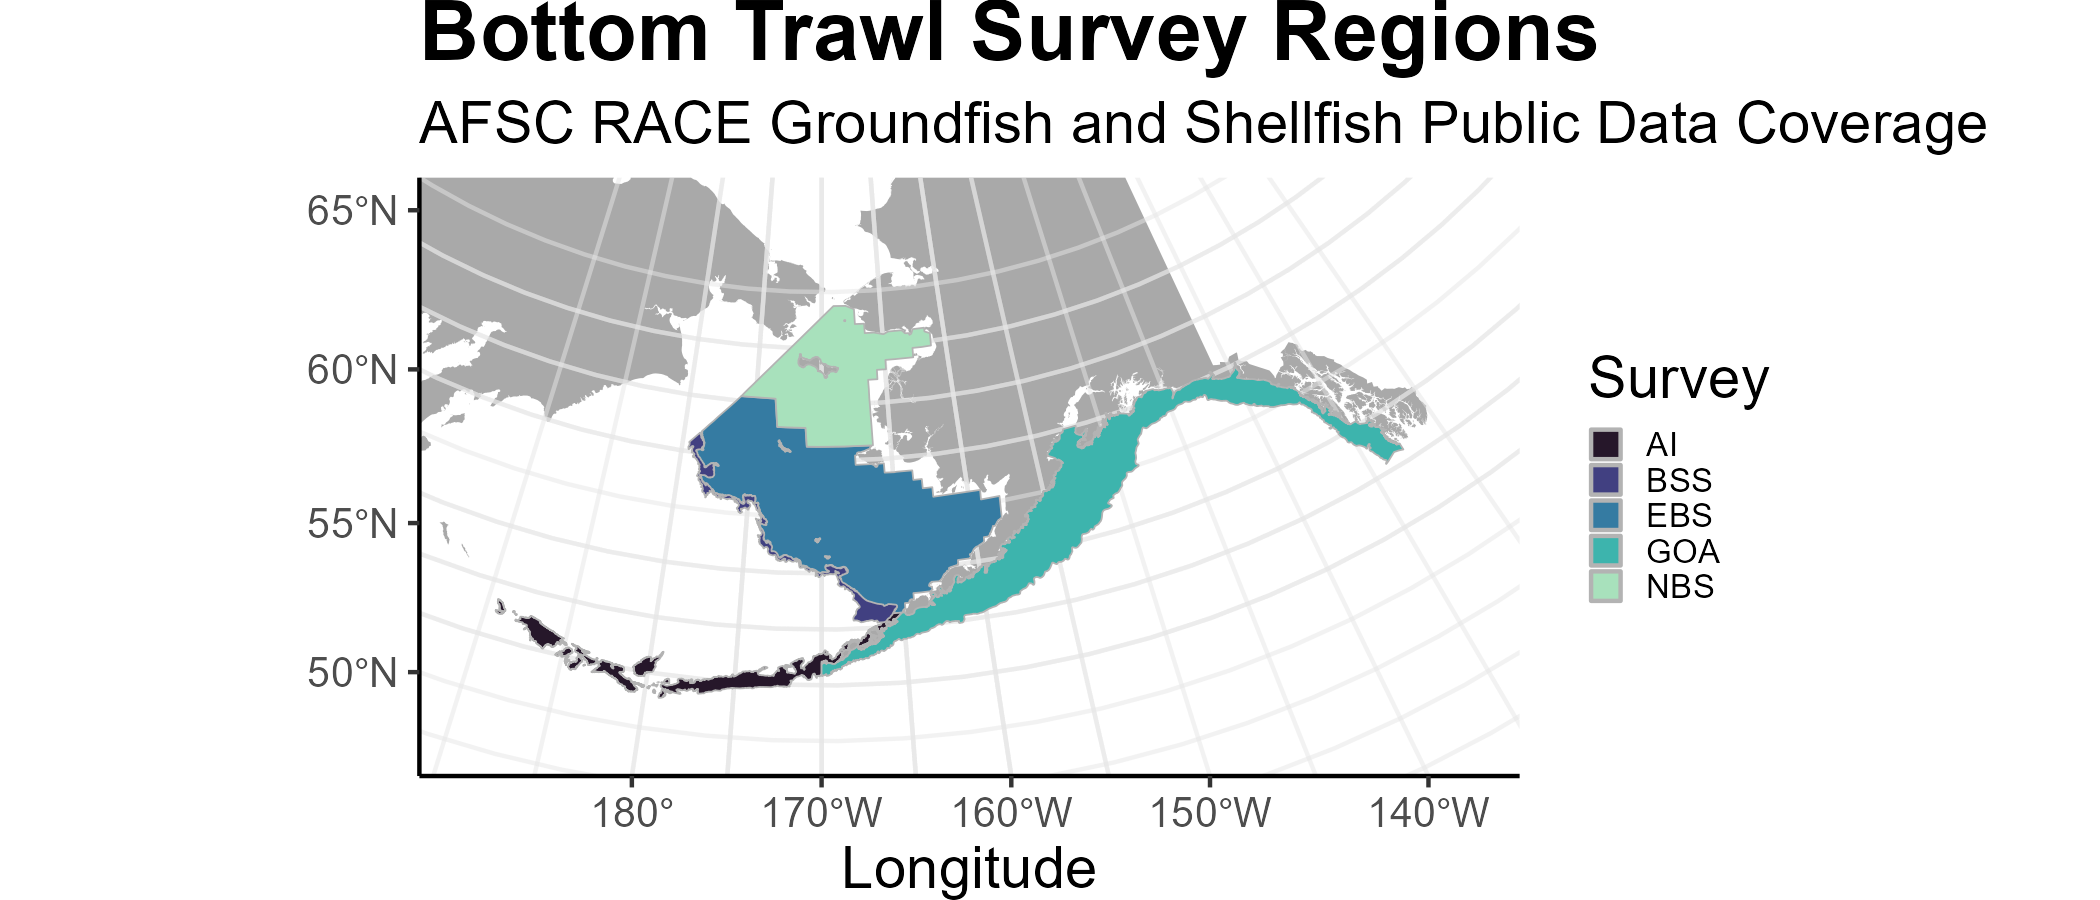
\includegraphics[width=7in,height=\textheight]{content/../img/survey_plot.png}

Each survey conducted by the
\href{https://www.fisheries.noaa.gov/alaska/population-assessments/north-pacific-groundfish-stock-assessments-and-fishery-evaluation}{Groundfish
Assessment Program} are multispecies bottom trawl surveys. We collect
environmental and biological data to assess how climate variability and
\href{https://www.fisheries.noaa.gov/alaska/ecosystems/habitat-and-ecological-processes-research-regarding-loss-sea-ice}{loss
of sea} ice are affecting bottom-dwelling marine life on the Bering Sea
shelf. We monitor trends in the distribution (location and movement
patterns) and abundance of groundfish and crab species as well as
oceanographic data (e.g., water temperature, depth). We collect
biological information such as organism weight, length, stomachs to
learn about diets, and
\href{https://www.fisheries.noaa.gov/alaska/science-data/alaska-age-and-growth-procedures-otolith-examination}{otoliths}
to
\href{https://www.fisheries.noaa.gov/alaska/science-data/fish-otolith-chronologies}{determine
fish ages}. We use this information in
\href{https://www.fisheries.noaa.gov/alaska/population-assessments/north-pacific-groundfish-stock-assessments-and-fishery-evaluation}{annual
stock assessments} and to assess the state of the ecosystem. This
research is conducted on fishing industry contract vessels.

\global\setlength{\Oldarrayrulewidth}{\arrayrulewidth}

\global\setlength{\Oldtabcolsep}{\tabcolsep}

\setlength{\tabcolsep}{0pt}

\renewcommand*{\arraystretch}{1.5}



\providecommand{\ascline}[3]{\noalign{\global\arrayrulewidth #1}\arrayrulecolor[HTML]{#2}\cline{#3}}

\begin{longtable}[c]{|p{1.50in}|p{0.91in}|p{0.72in}|p{0.48in}|p{0.52in}|p{0.83in}|p{0.88in}}
\caption{Survey summary stats}\tabularnewline




\hhline{>{\arrayrulecolor[HTML]{000000}\global\arrayrulewidth=0pt}->{\arrayrulecolor[HTML]{000000}\global\arrayrulewidth=0pt}->{\arrayrulecolor[HTML]{000000}\global\arrayrulewidth=0pt}->{\arrayrulecolor[HTML]{000000}\global\arrayrulewidth=0pt}->{\arrayrulecolor[HTML]{000000}\global\arrayrulewidth=0pt}->{\arrayrulecolor[HTML]{000000}\global\arrayrulewidth=0pt}->{\arrayrulecolor[HTML]{000000}\global\arrayrulewidth=0pt}-}

\multicolumn{1}{>{\cellcolor[HTML]{CFCFCF}\raggedright}m{\dimexpr 1.5in+0\tabcolsep}}{\textcolor[HTML]{000000}{\fontsize{10}{10}\selectfont{\textbf{Survey}}}} & \multicolumn{1}{>{\cellcolor[HTML]{CFCFCF}\raggedleft}m{\dimexpr 0.91in+0\tabcolsep}}{\textcolor[HTML]{000000}{\fontsize{10}{10}\selectfont{\textbf{Survey\ Definition\ ID}}}} & \multicolumn{1}{>{\cellcolor[HTML]{CFCFCF}\raggedright}m{\dimexpr 0.72in+0\tabcolsep}}{\textcolor[HTML]{000000}{\fontsize{10}{10}\selectfont{\textbf{Years}}}} & \multicolumn{1}{>{\cellcolor[HTML]{CFCFCF}\raggedright}m{\dimexpr 0.48in+0\tabcolsep}}{\textcolor[HTML]{000000}{\fontsize{10}{10}\selectfont{\textbf{Depth\ (m)}}}} & \multicolumn{1}{>{\cellcolor[HTML]{CFCFCF}\raggedright}m{\dimexpr 0.52in+0\tabcolsep}}{\textcolor[HTML]{000000}{\fontsize{10}{10}\selectfont{\textbf{Area\ (km2)}}}} & \multicolumn{1}{>{\cellcolor[HTML]{CFCFCF}\raggedleft}m{\dimexpr 0.83in+0\tabcolsep}}{\textcolor[HTML]{000000}{\fontsize{10}{10}\selectfont{\textbf{\#\ Statistical\ Areas}}}} & \multicolumn{1}{>{\cellcolor[HTML]{CFCFCF}\raggedleft}m{\dimexpr 0.88in+0\tabcolsep}}{\textcolor[HTML]{000000}{\fontsize{10}{10}\selectfont{\textbf{\#\ Possible\ Stations}}}} \\

\noalign{\global\arrayrulewidth 0pt}\arrayrulecolor[HTML]{000000}

\endfirsthead 

\hhline{>{\arrayrulecolor[HTML]{000000}\global\arrayrulewidth=0pt}->{\arrayrulecolor[HTML]{000000}\global\arrayrulewidth=0pt}->{\arrayrulecolor[HTML]{000000}\global\arrayrulewidth=0pt}->{\arrayrulecolor[HTML]{000000}\global\arrayrulewidth=0pt}->{\arrayrulecolor[HTML]{000000}\global\arrayrulewidth=0pt}->{\arrayrulecolor[HTML]{000000}\global\arrayrulewidth=0pt}->{\arrayrulecolor[HTML]{000000}\global\arrayrulewidth=0pt}-}

\multicolumn{1}{>{\cellcolor[HTML]{CFCFCF}\raggedright}m{\dimexpr 1.5in+0\tabcolsep}}{\textcolor[HTML]{000000}{\fontsize{10}{10}\selectfont{\textbf{Survey}}}} & \multicolumn{1}{>{\cellcolor[HTML]{CFCFCF}\raggedleft}m{\dimexpr 0.91in+0\tabcolsep}}{\textcolor[HTML]{000000}{\fontsize{10}{10}\selectfont{\textbf{Survey\ Definition\ ID}}}} & \multicolumn{1}{>{\cellcolor[HTML]{CFCFCF}\raggedright}m{\dimexpr 0.72in+0\tabcolsep}}{\textcolor[HTML]{000000}{\fontsize{10}{10}\selectfont{\textbf{Years}}}} & \multicolumn{1}{>{\cellcolor[HTML]{CFCFCF}\raggedright}m{\dimexpr 0.48in+0\tabcolsep}}{\textcolor[HTML]{000000}{\fontsize{10}{10}\selectfont{\textbf{Depth\ (m)}}}} & \multicolumn{1}{>{\cellcolor[HTML]{CFCFCF}\raggedright}m{\dimexpr 0.52in+0\tabcolsep}}{\textcolor[HTML]{000000}{\fontsize{10}{10}\selectfont{\textbf{Area\ (km2)}}}} & \multicolumn{1}{>{\cellcolor[HTML]{CFCFCF}\raggedleft}m{\dimexpr 0.83in+0\tabcolsep}}{\textcolor[HTML]{000000}{\fontsize{10}{10}\selectfont{\textbf{\#\ Statistical\ Areas}}}} & \multicolumn{1}{>{\cellcolor[HTML]{CFCFCF}\raggedleft}m{\dimexpr 0.88in+0\tabcolsep}}{\textcolor[HTML]{000000}{\fontsize{10}{10}\selectfont{\textbf{\#\ Possible\ Stations}}}} \\

\noalign{\global\arrayrulewidth 0pt}\arrayrulecolor[HTML]{000000}

\endhead



\multicolumn{1}{>{\cellcolor[HTML]{EFEFEF}\raggedright}m{\dimexpr 1.5in+0\tabcolsep}}{\textcolor[HTML]{000000}{\fontsize{10}{10}\selectfont{Aleutian}}\textcolor[HTML]{000000}{\fontsize{10}{10}\selectfont{\ }}\textcolor[HTML]{000000}{\fontsize{10}{10}\selectfont{Islands}}\textcolor[HTML]{000000}{\fontsize{10}{10}\selectfont{\ }}\textcolor[HTML]{000000}{\fontsize{10}{10}\selectfont{Bottom}}\textcolor[HTML]{000000}{\fontsize{10}{10}\selectfont{\ }}\textcolor[HTML]{000000}{\fontsize{10}{10}\selectfont{Trawl}}\textcolor[HTML]{000000}{\fontsize{10}{10}\selectfont{\ }}\textcolor[HTML]{000000}{\fontsize{10}{10}\selectfont{Survey}}} & \multicolumn{1}{>{\cellcolor[HTML]{EFEFEF}\centering}m{\dimexpr 0.91in+0\tabcolsep}}{\textcolor[HTML]{000000}{\fontsize{10}{10}\selectfont{52}}} & \multicolumn{1}{>{\cellcolor[HTML]{EFEFEF}\raggedright}m{\dimexpr 0.72in+0\tabcolsep}}{\textcolor[HTML]{000000}{\fontsize{10}{10}\selectfont{2022}}\textcolor[HTML]{000000}{\fontsize{10}{10}\selectfont{\ }}\textcolor[HTML]{000000}{\fontsize{10}{10}\selectfont{-}}\textcolor[HTML]{000000}{\fontsize{10}{10}\selectfont{\ }}\textcolor[HTML]{000000}{\fontsize{10}{10}\selectfont{1980}}\textcolor[HTML]{000000}{\fontsize{10}{10}\selectfont{\ }}\textcolor[HTML]{000000}{\fontsize{10}{10}\selectfont{(16)}}} & \multicolumn{1}{>{\cellcolor[HTML]{EFEFEF}\raggedright}m{\dimexpr 0.48in+0\tabcolsep}}{\textcolor[HTML]{000000}{\fontsize{10}{10}\selectfont{1}}\textcolor[HTML]{000000}{\fontsize{10}{10}\selectfont{\ }}\textcolor[HTML]{000000}{\fontsize{10}{10}\selectfont{-}}\textcolor[HTML]{000000}{\fontsize{10}{10}\selectfont{\ }}\textcolor[HTML]{000000}{\fontsize{10}{10}\selectfont{500}}} & \multicolumn{1}{>{\cellcolor[HTML]{EFEFEF}\raggedright}m{\dimexpr 0.52in+0\tabcolsep}}{\textcolor[HTML]{000000}{\fontsize{10}{10}\selectfont{64,415.0}}} & \multicolumn{1}{>{\cellcolor[HTML]{EFEFEF}\raggedleft}m{\dimexpr 0.83in+0\tabcolsep}}{\textcolor[HTML]{000000}{\fontsize{10}{10}\selectfont{80}}} & \multicolumn{1}{>{\cellcolor[HTML]{EFEFEF}\raggedleft}m{\dimexpr 0.88in+0\tabcolsep}}{\textcolor[HTML]{000000}{\fontsize{10}{10}\selectfont{1,312}}} \\

\noalign{\global\arrayrulewidth 0pt}\arrayrulecolor[HTML]{000000}





\multicolumn{1}{>{\raggedright}m{\dimexpr 1.5in+0\tabcolsep}}{\textcolor[HTML]{000000}{\fontsize{10}{10}\selectfont{Eastern}}\textcolor[HTML]{000000}{\fontsize{10}{10}\selectfont{\ }}\textcolor[HTML]{000000}{\fontsize{10}{10}\selectfont{Bering}}\textcolor[HTML]{000000}{\fontsize{10}{10}\selectfont{\ }}\textcolor[HTML]{000000}{\fontsize{10}{10}\selectfont{Sea}}\textcolor[HTML]{000000}{\fontsize{10}{10}\selectfont{\ }}\textcolor[HTML]{000000}{\fontsize{10}{10}\selectfont{Slope}}\textcolor[HTML]{000000}{\fontsize{10}{10}\selectfont{\ }}\textcolor[HTML]{000000}{\fontsize{10}{10}\selectfont{Bottom}}\textcolor[HTML]{000000}{\fontsize{10}{10}\selectfont{\ }}\textcolor[HTML]{000000}{\fontsize{10}{10}\selectfont{Trawl}}\textcolor[HTML]{000000}{\fontsize{10}{10}\selectfont{\ }}\textcolor[HTML]{000000}{\fontsize{10}{10}\selectfont{Survey}}} & \multicolumn{1}{>{\centering}m{\dimexpr 0.91in+0\tabcolsep}}{\textcolor[HTML]{000000}{\fontsize{10}{10}\selectfont{78}}} & \multicolumn{1}{>{\raggedright}m{\dimexpr 0.72in+0\tabcolsep}}{\textcolor[HTML]{000000}{\fontsize{10}{10}\selectfont{2016}}\textcolor[HTML]{000000}{\fontsize{10}{10}\selectfont{\ }}\textcolor[HTML]{000000}{\fontsize{10}{10}\selectfont{-}}\textcolor[HTML]{000000}{\fontsize{10}{10}\selectfont{\ }}\textcolor[HTML]{000000}{\fontsize{10}{10}\selectfont{2002}}\textcolor[HTML]{000000}{\fontsize{10}{10}\selectfont{\ }}\textcolor[HTML]{000000}{\fontsize{10}{10}\selectfont{(6)}}} & \multicolumn{1}{>{\raggedright}m{\dimexpr 0.48in+0\tabcolsep}}{\textcolor[HTML]{000000}{\fontsize{10}{10}\selectfont{201}}\textcolor[HTML]{000000}{\fontsize{10}{10}\selectfont{\ }}\textcolor[HTML]{000000}{\fontsize{10}{10}\selectfont{-}}\textcolor[HTML]{000000}{\fontsize{10}{10}\selectfont{\ }}\textcolor[HTML]{000000}{\fontsize{10}{10}\selectfont{800}}} & \multicolumn{1}{>{\raggedright}m{\dimexpr 0.52in+0\tabcolsep}}{\textcolor[HTML]{000000}{\fontsize{10}{10}\selectfont{21,134.2}}} & \multicolumn{1}{>{\raggedleft}m{\dimexpr 0.83in+0\tabcolsep}}{\textcolor[HTML]{000000}{\fontsize{10}{10}\selectfont{4}}} & \multicolumn{1}{>{\raggedleft}m{\dimexpr 0.88in+0\tabcolsep}}{\textcolor[HTML]{000000}{\fontsize{10}{10}\selectfont{}}} \\

\noalign{\global\arrayrulewidth 0pt}\arrayrulecolor[HTML]{000000}





\multicolumn{1}{>{\cellcolor[HTML]{EFEFEF}\raggedright}m{\dimexpr 1.5in+0\tabcolsep}}{\textcolor[HTML]{000000}{\fontsize{10}{10}\selectfont{Eastern}}\textcolor[HTML]{000000}{\fontsize{10}{10}\selectfont{\ }}\textcolor[HTML]{000000}{\fontsize{10}{10}\selectfont{Bering}}\textcolor[HTML]{000000}{\fontsize{10}{10}\selectfont{\ }}\textcolor[HTML]{000000}{\fontsize{10}{10}\selectfont{Sea}}\textcolor[HTML]{000000}{\fontsize{10}{10}\selectfont{\ }}\textcolor[HTML]{000000}{\fontsize{10}{10}\selectfont{Crab/Groundfish}}\textcolor[HTML]{000000}{\fontsize{10}{10}\selectfont{\ }}\textcolor[HTML]{000000}{\fontsize{10}{10}\selectfont{Bottom}}\textcolor[HTML]{000000}{\fontsize{10}{10}\selectfont{\ }}\textcolor[HTML]{000000}{\fontsize{10}{10}\selectfont{Trawl}}\textcolor[HTML]{000000}{\fontsize{10}{10}\selectfont{\ }}\textcolor[HTML]{000000}{\fontsize{10}{10}\selectfont{Survey}}} & \multicolumn{1}{>{\cellcolor[HTML]{EFEFEF}\centering}m{\dimexpr 0.91in+0\tabcolsep}}{\textcolor[HTML]{000000}{\fontsize{10}{10}\selectfont{98}}} & \multicolumn{1}{>{\cellcolor[HTML]{EFEFEF}\raggedright}m{\dimexpr 0.72in+0\tabcolsep}}{\textcolor[HTML]{000000}{\fontsize{10}{10}\selectfont{2023}}\textcolor[HTML]{000000}{\fontsize{10}{10}\selectfont{\ }}\textcolor[HTML]{000000}{\fontsize{10}{10}\selectfont{-}}\textcolor[HTML]{000000}{\fontsize{10}{10}\selectfont{\ }}\textcolor[HTML]{000000}{\fontsize{10}{10}\selectfont{1982}}\textcolor[HTML]{000000}{\fontsize{10}{10}\selectfont{\ }}\textcolor[HTML]{000000}{\fontsize{10}{10}\selectfont{(41)}}} & \multicolumn{1}{>{\cellcolor[HTML]{EFEFEF}\raggedright}m{\dimexpr 0.48in+0\tabcolsep}}{\textcolor[HTML]{000000}{\fontsize{10}{10}\selectfont{1}}\textcolor[HTML]{000000}{\fontsize{10}{10}\selectfont{\ }}\textcolor[HTML]{000000}{\fontsize{10}{10}\selectfont{-}}\textcolor[HTML]{000000}{\fontsize{10}{10}\selectfont{\ }}\textcolor[HTML]{000000}{\fontsize{10}{10}\selectfont{200}}} & \multicolumn{1}{>{\cellcolor[HTML]{EFEFEF}\raggedright}m{\dimexpr 0.52in+0\tabcolsep}}{\textcolor[HTML]{000000}{\fontsize{10}{10}\selectfont{492,989.9}}} & \multicolumn{1}{>{\cellcolor[HTML]{EFEFEF}\raggedleft}m{\dimexpr 0.83in+0\tabcolsep}}{\textcolor[HTML]{000000}{\fontsize{10}{10}\selectfont{29}}} & \multicolumn{1}{>{\cellcolor[HTML]{EFEFEF}\raggedleft}m{\dimexpr 0.88in+0\tabcolsep}}{\textcolor[HTML]{000000}{\fontsize{10}{10}\selectfont{515}}} \\

\noalign{\global\arrayrulewidth 0pt}\arrayrulecolor[HTML]{000000}





\multicolumn{1}{>{\raggedright}m{\dimexpr 1.5in+0\tabcolsep}}{\textcolor[HTML]{000000}{\fontsize{10}{10}\selectfont{Gulf}}\textcolor[HTML]{000000}{\fontsize{10}{10}\selectfont{\ }}\textcolor[HTML]{000000}{\fontsize{10}{10}\selectfont{of}}\textcolor[HTML]{000000}{\fontsize{10}{10}\selectfont{\ }}\textcolor[HTML]{000000}{\fontsize{10}{10}\selectfont{Alaska}}\textcolor[HTML]{000000}{\fontsize{10}{10}\selectfont{\ }}\textcolor[HTML]{000000}{\fontsize{10}{10}\selectfont{Bottom}}\textcolor[HTML]{000000}{\fontsize{10}{10}\selectfont{\ }}\textcolor[HTML]{000000}{\fontsize{10}{10}\selectfont{Trawl}}\textcolor[HTML]{000000}{\fontsize{10}{10}\selectfont{\ }}\textcolor[HTML]{000000}{\fontsize{10}{10}\selectfont{Survey}}} & \multicolumn{1}{>{\centering}m{\dimexpr 0.91in+0\tabcolsep}}{\textcolor[HTML]{000000}{\fontsize{10}{10}\selectfont{47}}} & \multicolumn{1}{>{\raggedright}m{\dimexpr 0.72in+0\tabcolsep}}{\textcolor[HTML]{000000}{\fontsize{10}{10}\selectfont{2023}}\textcolor[HTML]{000000}{\fontsize{10}{10}\selectfont{\ }}\textcolor[HTML]{000000}{\fontsize{10}{10}\selectfont{-}}\textcolor[HTML]{000000}{\fontsize{10}{10}\selectfont{\ }}\textcolor[HTML]{000000}{\fontsize{10}{10}\selectfont{1984}}\textcolor[HTML]{000000}{\fontsize{10}{10}\selectfont{\ }}\textcolor[HTML]{000000}{\fontsize{10}{10}\selectfont{(18)}}} & \multicolumn{1}{>{\raggedright}m{\dimexpr 0.48in+0\tabcolsep}}{\textcolor[HTML]{000000}{\fontsize{10}{10}\selectfont{1}}\textcolor[HTML]{000000}{\fontsize{10}{10}\selectfont{\ }}\textcolor[HTML]{000000}{\fontsize{10}{10}\selectfont{-}}\textcolor[HTML]{000000}{\fontsize{10}{10}\selectfont{\ }}\textcolor[HTML]{000000}{\fontsize{10}{10}\selectfont{1,000}}} & \multicolumn{1}{>{\raggedright}m{\dimexpr 0.52in+0\tabcolsep}}{\textcolor[HTML]{000000}{\fontsize{10}{10}\selectfont{314,087.4}}} & \multicolumn{1}{>{\raggedleft}m{\dimexpr 0.83in+0\tabcolsep}}{\textcolor[HTML]{000000}{\fontsize{10}{10}\selectfont{39}}} & \multicolumn{1}{>{\raggedleft}m{\dimexpr 0.88in+0\tabcolsep}}{\textcolor[HTML]{000000}{\fontsize{10}{10}\selectfont{6,939}}} \\

\noalign{\global\arrayrulewidth 0pt}\arrayrulecolor[HTML]{000000}





\multicolumn{1}{>{\cellcolor[HTML]{EFEFEF}\raggedright}m{\dimexpr 1.5in+0\tabcolsep}}{\textcolor[HTML]{000000}{\fontsize{10}{10}\selectfont{Northern}}\textcolor[HTML]{000000}{\fontsize{10}{10}\selectfont{\ }}\textcolor[HTML]{000000}{\fontsize{10}{10}\selectfont{Bering}}\textcolor[HTML]{000000}{\fontsize{10}{10}\selectfont{\ }}\textcolor[HTML]{000000}{\fontsize{10}{10}\selectfont{Sea}}\textcolor[HTML]{000000}{\fontsize{10}{10}\selectfont{\ }}\textcolor[HTML]{000000}{\fontsize{10}{10}\selectfont{Crab/Groundfish}}\textcolor[HTML]{000000}{\fontsize{10}{10}\selectfont{\ }}\textcolor[HTML]{000000}{\fontsize{10}{10}\selectfont{Survey}}\textcolor[HTML]{000000}{\fontsize{10}{10}\selectfont{\ }}\textcolor[HTML]{000000}{\fontsize{10}{10}\selectfont{-}}\textcolor[HTML]{000000}{\fontsize{10}{10}\selectfont{\ }}\textcolor[HTML]{000000}{\fontsize{10}{10}\selectfont{Eastern}}\textcolor[HTML]{000000}{\fontsize{10}{10}\selectfont{\ }}\textcolor[HTML]{000000}{\fontsize{10}{10}\selectfont{Bering}}\textcolor[HTML]{000000}{\fontsize{10}{10}\selectfont{\ }}\textcolor[HTML]{000000}{\fontsize{10}{10}\selectfont{Sea}}\textcolor[HTML]{000000}{\fontsize{10}{10}\selectfont{\ }}\textcolor[HTML]{000000}{\fontsize{10}{10}\selectfont{Shelf}}\textcolor[HTML]{000000}{\fontsize{10}{10}\selectfont{\ }}\textcolor[HTML]{000000}{\fontsize{10}{10}\selectfont{Survey}}\textcolor[HTML]{000000}{\fontsize{10}{10}\selectfont{\ }}\textcolor[HTML]{000000}{\fontsize{10}{10}\selectfont{Extension}}} & \multicolumn{1}{>{\cellcolor[HTML]{EFEFEF}\centering}m{\dimexpr 0.91in+0\tabcolsep}}{\textcolor[HTML]{000000}{\fontsize{10}{10}\selectfont{143}}} & \multicolumn{1}{>{\cellcolor[HTML]{EFEFEF}\raggedright}m{\dimexpr 0.72in+0\tabcolsep}}{\textcolor[HTML]{000000}{\fontsize{10}{10}\selectfont{2023}}\textcolor[HTML]{000000}{\fontsize{10}{10}\selectfont{\ }}\textcolor[HTML]{000000}{\fontsize{10}{10}\selectfont{-}}\textcolor[HTML]{000000}{\fontsize{10}{10}\selectfont{\ }}\textcolor[HTML]{000000}{\fontsize{10}{10}\selectfont{2010}}\textcolor[HTML]{000000}{\fontsize{10}{10}\selectfont{\ }}\textcolor[HTML]{000000}{\fontsize{10}{10}\selectfont{(6)}}} & \multicolumn{1}{>{\cellcolor[HTML]{EFEFEF}\raggedright}m{\dimexpr 0.48in+0\tabcolsep}}{\textcolor[HTML]{000000}{\fontsize{10}{10}\selectfont{1}}\textcolor[HTML]{000000}{\fontsize{10}{10}\selectfont{\ }}\textcolor[HTML]{000000}{\fontsize{10}{10}\selectfont{-}}\textcolor[HTML]{000000}{\fontsize{10}{10}\selectfont{\ }}\textcolor[HTML]{000000}{\fontsize{10}{10}\selectfont{100}}} & \multicolumn{1}{>{\cellcolor[HTML]{EFEFEF}\raggedright}m{\dimexpr 0.52in+0\tabcolsep}}{\textcolor[HTML]{000000}{\fontsize{10}{10}\selectfont{198,866.8}}} & \multicolumn{1}{>{\cellcolor[HTML]{EFEFEF}\raggedleft}m{\dimexpr 0.83in+0\tabcolsep}}{\textcolor[HTML]{000000}{\fontsize{10}{10}\selectfont{4}}} & \multicolumn{1}{>{\cellcolor[HTML]{EFEFEF}\raggedleft}m{\dimexpr 0.88in+0\tabcolsep}}{\textcolor[HTML]{000000}{\fontsize{10}{10}\selectfont{144}}} \\

\noalign{\global\arrayrulewidth 0pt}\arrayrulecolor[HTML]{000000}





\end{longtable}



\arrayrulecolor[HTML]{000000}

\global\setlength{\arrayrulewidth}{\Oldarrayrulewidth}

\global\setlength{\tabcolsep}{\Oldtabcolsep}

\renewcommand*{\arraystretch}{1}

\hypertarget{aleutian-islands}{%
\subsection{\texorpdfstring{\textbf{Aleutian
Islands}}{Aleutian Islands}}\label{aleutian-islands}}

(Von Szalay and Raring, 2020)

\begin{itemize}
\tightlist
\item
  Upper Continental Slope of the Aleutian Islands from Unimak Pass to
  Stalemate Bank
\item
  Triennial (1990s)/Biennial since 2000 in even years, since 1992
\item
  Modified Index-Stratified Random of Successful Stations Survey Design
\item
  Important commercial fish species include Atka mackerel,
  \href{https://www.fisheries.noaa.gov/species/pacific-ocean-perch}{Pacific
  ocean perch},
  \href{https://www.fisheries.noaa.gov/species/alaska-pollock}{walleye
  pollock},
  \href{https://www.fisheries.noaa.gov/species/pacific-cod}{Pacific
  cod},
  \href{https://www.fisheries.noaa.gov/species/sablefish}{sablefish},
  and other rockfish species.
\end{itemize}

\hypertarget{gulf-of-alaska}{%
\subsection{\texorpdfstring{\textbf{Gulf of
Alaska}}{Gulf of Alaska}}\label{gulf-of-alaska}}

(Von Szalay and Raring, 2018)

\begin{itemize}
\tightlist
\item
  Continental Shelf and Upper Slope of the Gulf of Alaska extending from
  the Islands of Four Mountains 2,300 km east to Dixon Entrance
\item
  Triennial (1990s)/Biennial since 2001 in odd years, since 1991
\item
  Stratified Random Survey Design
\item
  Important commercial species in the Gulf of Alaska include
  \href{https://www.fisheries.noaa.gov/species/pacific-ocean-perch}{Pacific
  ocean perch},
  \href{https://www.fisheries.noaa.gov/species/alaska-pollock}{walleye
  pollock},
  \href{https://www.fisheries.noaa.gov/species/pacific-cod}{Pacific
  cod}, flatfish, and other rockfish species.
\end{itemize}

\hypertarget{eastern-bering-sea-shelf}{%
\subsection{\texorpdfstring{\textbf{Eastern Bering Sea
Shelf}}{Eastern Bering Sea Shelf}}\label{eastern-bering-sea-shelf}}

(Markowitz et al., 2023)

\begin{itemize}
\tightlist
\item
  The continental shelf of the eastern Bering Sea from the Aleutian
  Islands to the Bering Strait
\item
  Conducted annually since 1982.
\item
  Uses a stratified systematic sampling survey design with fixed
  stations at center of 20 x 20 nm grid.
\item
  Similar in design to the northern Bering Sea shelf bottom trawl
  survey.
\item
  Focus species for the Bering Sea include
  \href{https://www.fisheries.noaa.gov/species/alaska-pollock}{walleye
  pollock},
  \href{https://www.fisheries.noaa.gov/species/pacific-cod}{Pacific
  cod},
  \href{https://www.fisheries.noaa.gov/species/greenland-turbot}{Greenland
  turbot},
  \href{https://www.fisheries.noaa.gov/species/yellowfin-sole}{yellowfin
  sole},
  \href{https://www.fisheries.noaa.gov/species/rock-sole}{northern rock
  sole}, \href{https://www.fisheries.noaa.gov/species/red-king-crab}{red
  king crab}, and
  \href{https://www.fisheries.noaa.gov/species/alaska-snow-crab}{snow}
  and Tanner crabs.
\end{itemize}

\begin{figure}

{\centering 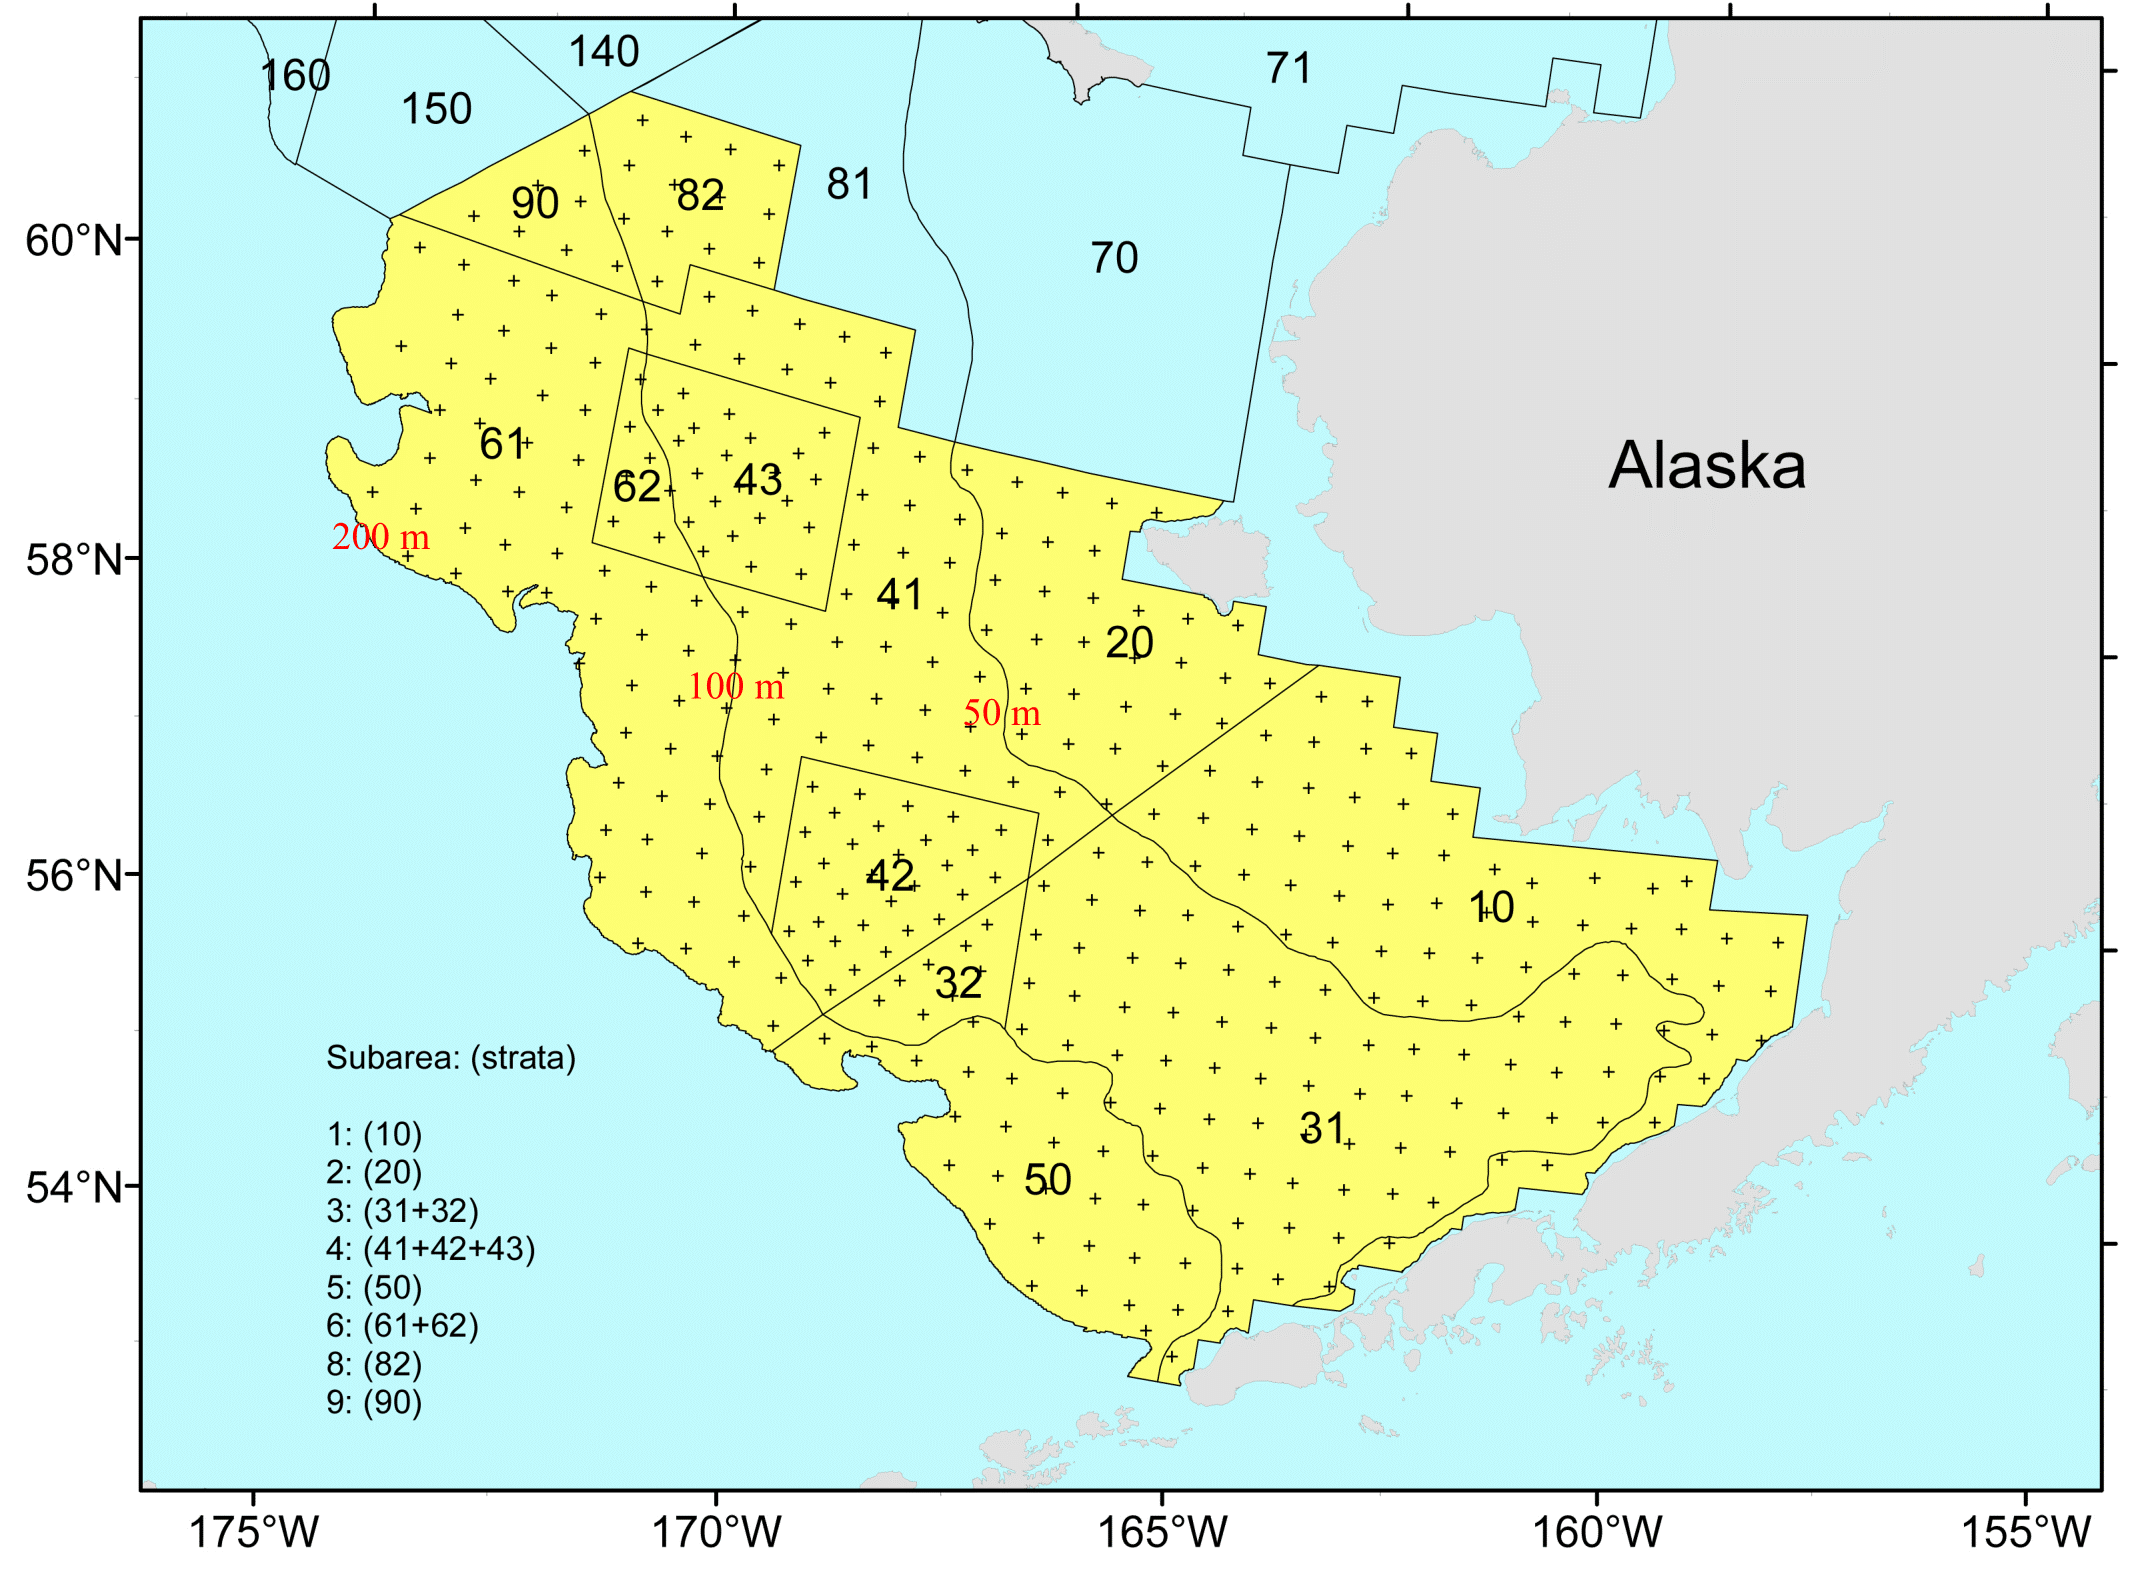
\includegraphics[width=7.19in,height=\textheight]{content/../img/ebs-strata.png}

}

\caption{Strata used in the Eastern Bering Sea Survey.}

\end{figure}

\hypertarget{northern-bering-sea}{%
\subsection{\texorpdfstring{\textbf{Northern Bering
Sea}}{Northern Bering Sea}}\label{northern-bering-sea}}

(Markowitz et al., 2023)

\begin{itemize}
\tightlist
\item
  The continental shelf of the northern Bering Sea, including the area
  north of St.~Lawrence Island and Norton Sound
\item
  Biennial/Annual; conducted intermittently since 2010
\item
  Uses a stratified systematic sampling survey design with fixed
  stations at center of 20 x 20 nm grid.
\item
  Similar in design to the eastern Bering Sea shelf bottom trawl survey.
\end{itemize}

\hypertarget{eastern-bering-sea-upper-continental-slope}{%
\subsection{\texorpdfstring{\textbf{Eastern Bering Sea Upper Continental
Slope}}{Eastern Bering Sea Upper Continental Slope}}\label{eastern-bering-sea-upper-continental-slope}}

(Hoff, 2016)

\begin{itemize}
\tightlist
\item
  The eastern Bering Sea upper continental slope survey area extends
  from Unalaska and Akutan Islands to the U.S.-Russian Maritime Boundary
  at 61° N near the International Date Line (166° E to 180° W) at depths
  from 200 to 1,200 m
\item
  Conducted intermittently since 2002 (funding dependent)
\item
  Modified Index-Stratified Random of Successful Stations Survey Design
\item
  Focus species for the Bering Sea slope include giant grenadier,
  \href{https://www.fisheries.noaa.gov/species/pacific-ocean-perch}{Pacific
  ocean perch}, popeye grenadier,
  \href{https://www.fisheries.noaa.gov/species/alaska-pollock}{walleye
  pollock}, and
  \href{https://www.fisheries.noaa.gov/species/arrowtooth-flounder}{arrowtooth
  flounder}.
\end{itemize}

\begin{figure}

{\centering 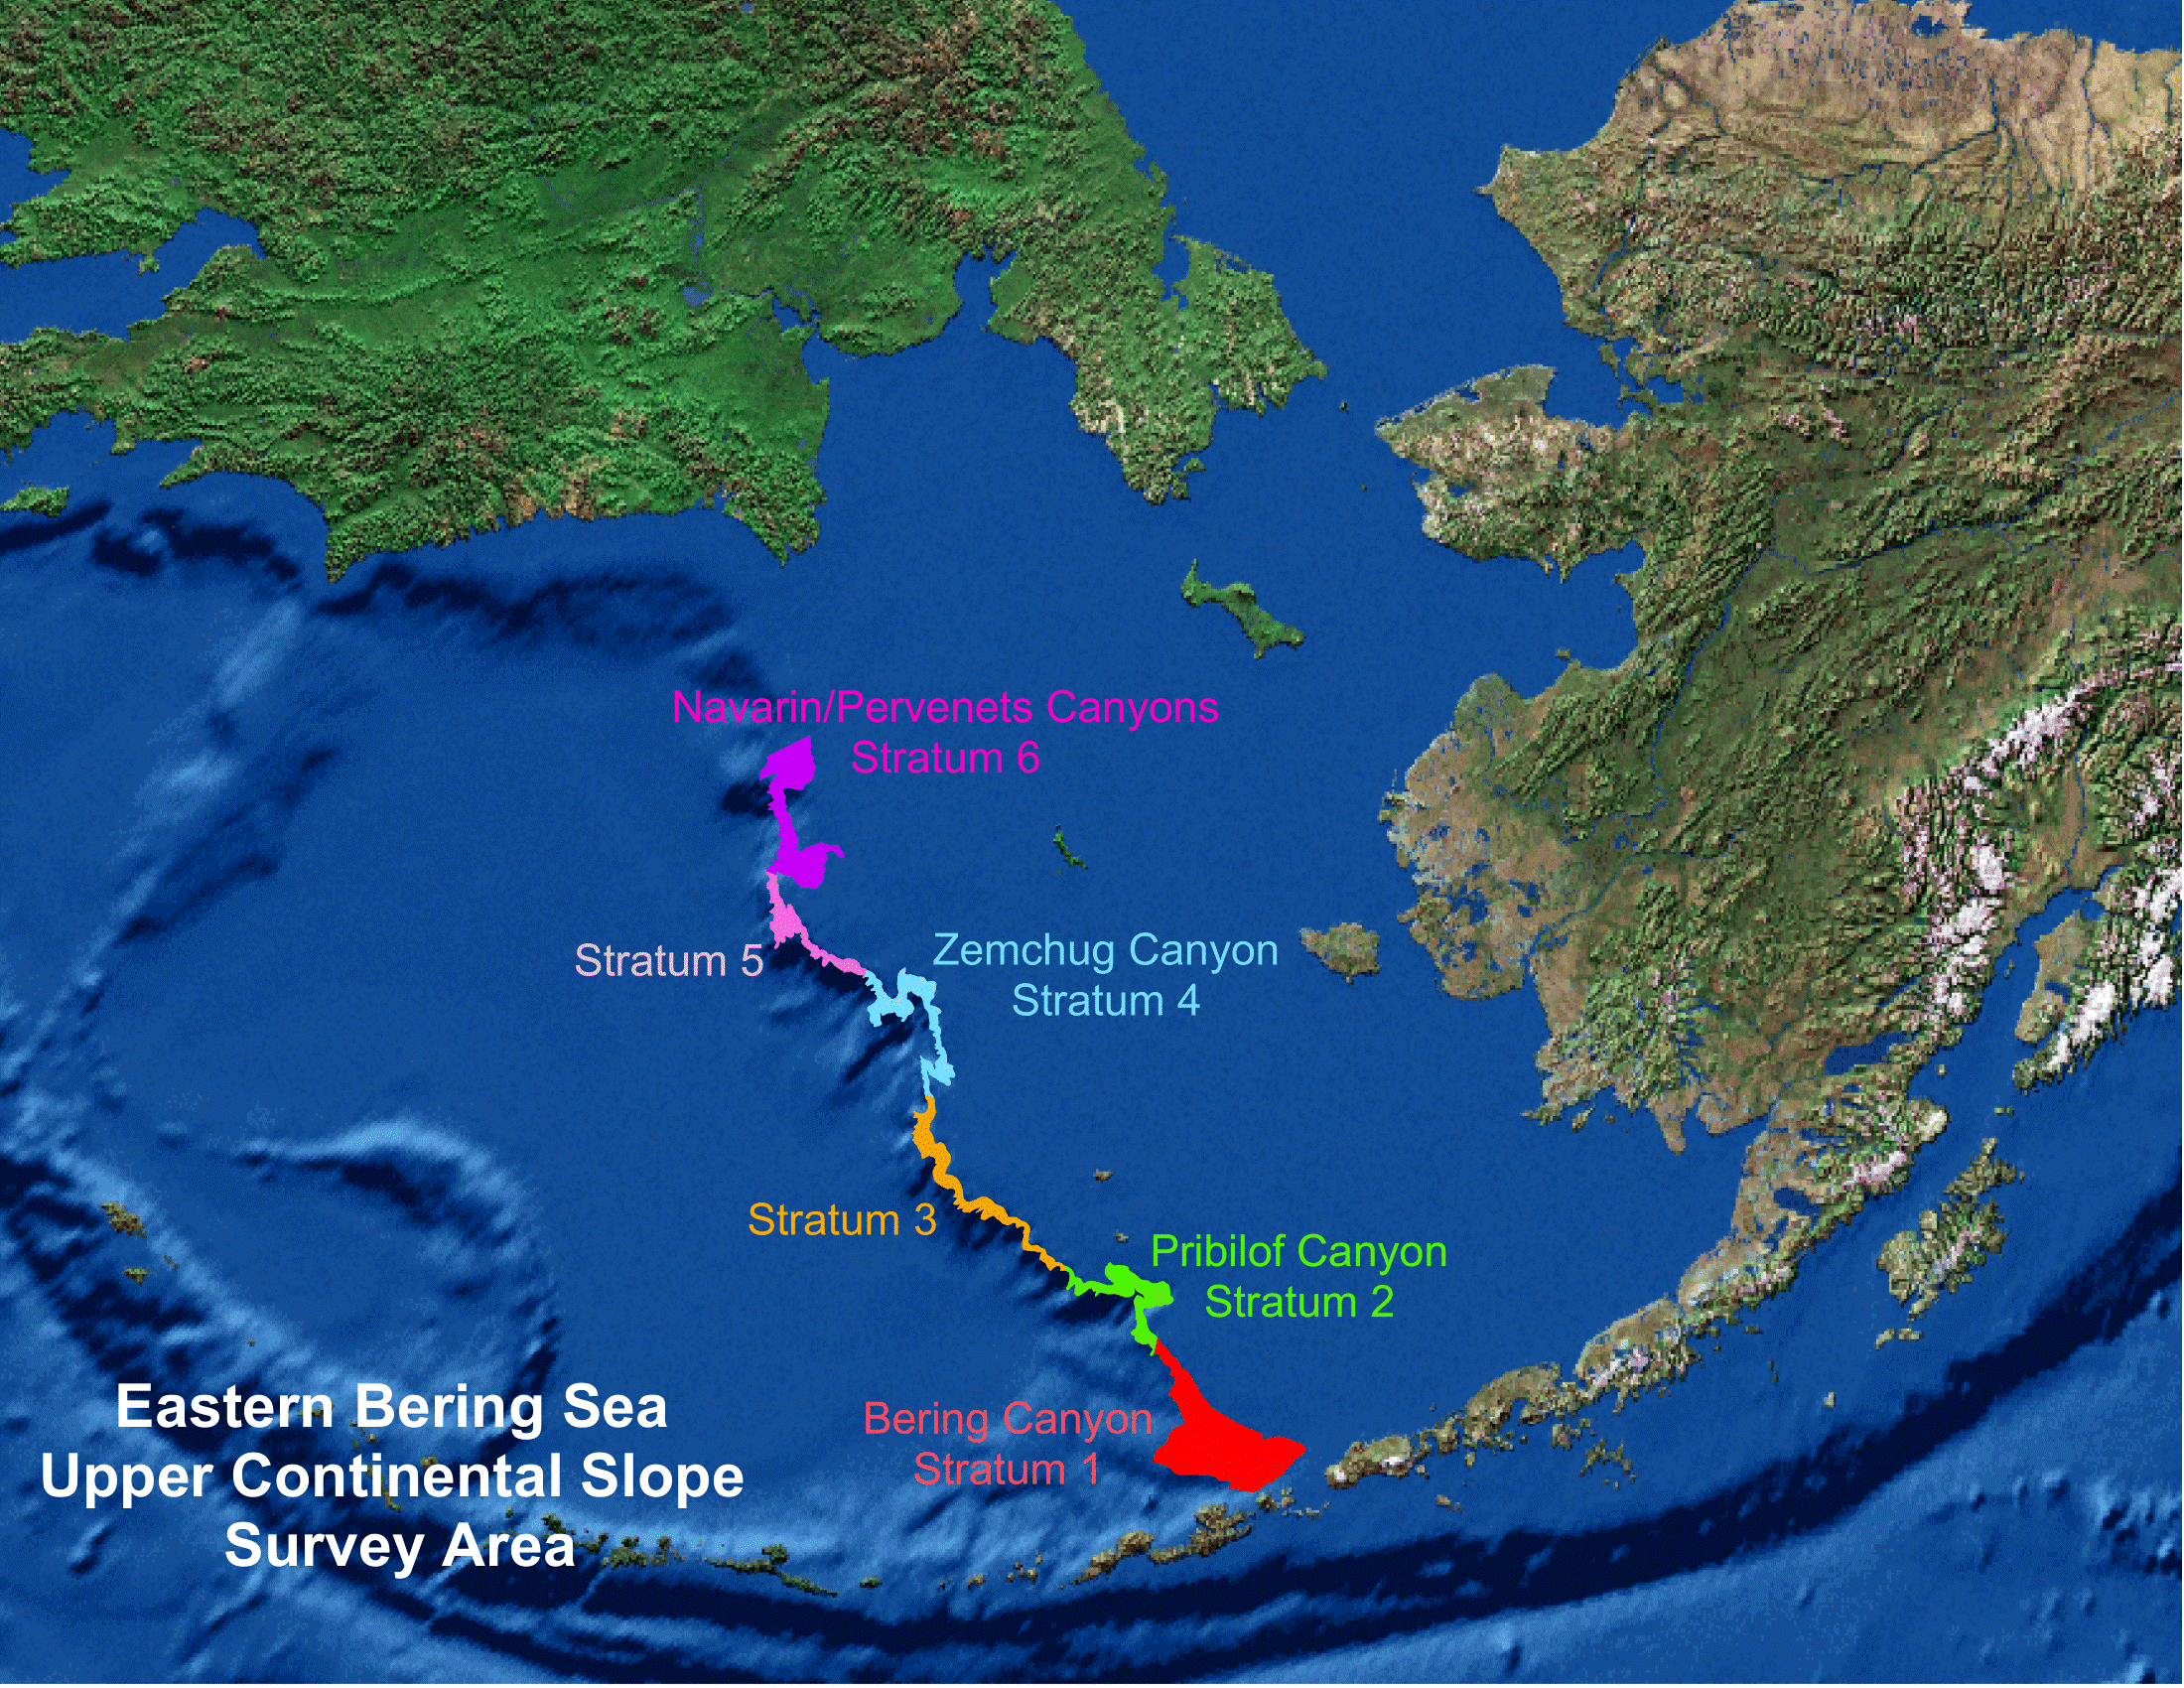
\includegraphics[width=7.33in,height=\textheight]{content/../img/bss-strata.png}

}

\caption{Strata used in the Bering Sea Slope Survey.}

\end{figure}

\hypertarget{workflow}{%
\chapter{Workflow}\label{workflow}}

\hypertarget{data-workflow-from-boat-to-production}{%
\section{Data workflow from boat to
production}\label{data-workflow-from-boat-to-production}}

\begin{figure}

{\centering 

\begin{figure}[H]

{\centering 
\includegraphics[width=14.65in,height=2.96in]{content/intro-workflow_files/figure-latex/mermaid-figure-1.png}

}

\end{figure}

}

\caption{\label{fig-workflow}Simplified data workflow from boat to
production.}

\end{figure}

\hypertarget{organization}{%
\section{Organization}\label{organization}}

The code/run.R script houses the sequence of programs that calculate the
standard data products resulting from the NOAA AFSC GAP bottom trawl
surveys. Standard data products are the CPUE, BIOMASS, SIZECOMP, and
AGECOMP tables in the GAP\_PRODUCTS Oracle schema. The tables are slated
to be updated twice a year, once after the survey season following
finalization of that summer's bottom trawl survey data to incorporate
the new catch, size, and effort data and once prior to an upcoming
survey to incorporate new age data that were processed after the prior
summer's survey season ended. This second pre-survey production run will
also incorporate changes in the data due to the specimen voucher process
as well as other post-hoc changes in the survey data.

Below is a summary of the workflow:

\begin{enumerate}
\def\labelenumi{\arabic{enumi}.}
\item
  Import versions of the tables in GAP\_PRODUCTS locally within the
  gap\_products repository to compare with the updated production
  tables. Any changes to a production table will be compared and checked
  to make sure those changes are intentional and documented.
\item
  Use the gapindex R package to calculate the four major standard data
  products: CPUE, BIOMASS, SIZECOMP, AGECOMP. These tables are compared
  and checked to their respective locally saved copies and any changes
  to the tables are vetted and documented. These tables are then
  uploaded to the GAP\_PRODUCTS Oracle schema.
\item
  Calculate the various materialized views for AKFIN and FOSS purposes.
  Since these are derivative of the tables in GAP\_PRODUCTS as well as
  other base tables in RACEBASE and RACE\_DATA, it is not necessary to
  check these views in addition to the data checks done in the previous
  steps.
\end{enumerate}

\hypertarget{data-levels}{%
\section{Data levels}\label{data-levels}}

GAP produces numerous data products that are subjected to different
levels of processing, ranging from raw to highly-derived. The
suitability of these data products for analysis varies and there is
ambiguity about which data products can be used for which purpose. This
ambiguity can create challenges in communicating about data products and
potentially lead to misunderstanding and misuse of data. One approach to
communicating about the level of processing applied to data products and
their suitability for analysis is to describe data products using a Data
Processing Level system. Data Processing Level systems are widely used
in earth system sciences to characterize the extent of processing that
has been applied to data products. For example, the NOAA National
Centers for Environmental Information (NCEI) Satellite Program uses a
Data Processing Level system to describe data on a scale of 0-4, where
Level 0 is raw data and Level 4 is model output or results from
analysis. Example of how
\href{https://ladsweb.modaps.eosdis.nasa.gov/search/}{NASA remote
sensing data products} are shared through a public data portal with
levels of data processing and documentation.

For more information, see
\href{https://docs.google.com/presentation/d/1rWSZpeghWJqzWMIa5oBc4BCoy-zy1Yue86RoTw58u6M/edit?usp=sharing}{Sean
Rohan's October 2022 SCRUGS presentation} on the topic.

\begin{itemize}
\tightlist
\item
  \textbf{Level 0}: Raw and unprocessed data. Ex: Data on the G drive,
  some tables in RACE\_DATA
\item
  \textbf{Level 1A}: Data products with QA/QC applied that may or may
  not be expanded to analysis units, but either not georeferenced or
  does not include full metadata. Ex: Some tables in RACE\_DATA and
  RACEBASE
\item
  \textbf{Level 2}: Analysis-ready data products that are derived for a
  standardized extent and account for zeros and missing/bad data. Ex:
  CPUE tables, some data products in public-facing archives and
  repositories
\item
  \textbf{Level 3}: Data products that are synthesized across a
  standardized extent, often inputs in a higher-level analytical
  product. Ex: Abundance indices, some data products in public-facing
  archives and repositories
\item
  \textbf{Level 4}: Analytically generated data products that are
  derived from lower-level data, often to inform management. Ex:
  Biological reference points from stock assessments, Essential Fish
  Habitat layers, indicators in Ecosystem Status Reports and Ecosystem
  and Socioeconomic Profiles
\end{itemize}

\hypertarget{news}{%
\chapter{News}\label{news}}

\hypertarget{future-plans}{%
\section{Future plans}\label{future-plans}}

\hypertarget{goa-2025-restratification-mock-data-for-testing}{%
\subsection{GOA 2025 Restratification -- Mock Data for
Testing}\label{goa-2025-restratification-mock-data-for-testing}}

The plan will be, once all are satisfied with the new GAP\_PRODUCTS
schema and tables, to sunset the historic product tables in 2024 and
proceed with only GAP\_PRODUCTS for the 2024 post-survey stock
assessment season.

\begin{itemize}
\item
  December 2023 - March 2024: Meeting between GAP and stock assessment
  groups in early December 2023 to update progress on the GAP\_PRODUCTS
  testing phase. \textbf{Deadline for Comments and Feedback on
  GAP\_PRODUCTS data structures is March 8, 2024.}
\item
  September 2024: GAP will only release data products according to the
  new standard. Current, historical data product tables will be archived
  in a new schema called "\textbf{GAP\_ARCHIVE}".
\end{itemize}

\hypertarget{previous-updates}{%
\section{Previous updates}\label{previous-updates}}

\begin{itemize}
\item
  September 2023: Provisional data product tables -- CPUE, BIOMASS,
  SIZECOMP, and AGECOMP -- as well as provisional support tables --
  AREA, STRATUM\_GROUPS, METADATA\_COLUMN, SPECIES\_YEAR, SURVEY\_DESIGN
  -- are available in the GAP\_PRODUCTS Oracle schema with updated 2023
  GOA and EBS survey data.

  \begin{itemize}
  \item
    Additionally, the inclusion of mock data for the under the new 2025
    GOA stratified random survey (labeled in the GAP\_PRODUCTS tables as
    YEAR 2025) will provide stock authors with the opportunity to
    interact with data from the new survey design to be implemented in
    2025.
  \item
    Provisional AKFIN and FOSS tables are also available in the
    GAP\_PRODUCTS Oracle schema. These include: AKFIN\_AGECOMP,
    AKFIN\_AREA, AKFIN\_BIOMASS, AKFIN\_CATCH, AKFIN\_CPUE,
    AKFIN\_CRUISE, AKFIN\_HAUL, AKFIN\_LENGTH, AKFIN\_METADATA\_COLUMN,
    AKFIN\_SIZECOMP, AKFIN\_SPECIMEN, AKFIN\_SURVEY\_DESIGN,
    AKFIN\_STRATUM\_GROUPS, FOSS\_CATCH, FOSS\_CPUE\_PRESONLY,
    FOSS\_HAUL, and FOSS\_TAXON\_GROUP.
  \end{itemize}
\item
  May 2023: Release of new, draft, standard data product tables,
  including restratified GOA data. Stock assessment authors will have
  the opportunity to explore differences between datasets, test
  workflows, and provide comments and issues during summer 2023.
\item
  February 2023: Decision was made to include the mock restratified GOA
  data with the development of the new consolidated standard data
  products.
\item
  December 2022:
  \href{https://docs.google.com/document/d/1AURrvC1na6TL1Um3p7018svBLDOnih_7nxxyRU34M0k/edit}{GAP
  and SSMA discuss} integration of the restratification of the GOA
  survey design into standard data products.

  \begin{itemize}
  \item
    Stock assessors requested a "dry run" test to work with new mock
    restratified GOA survey data before implementation of the new survey
    design.
  \item
    This prompted the postponement of the restratified GOA design to
    2025.
  \end{itemize}
\item
  October 2022: The data processes and index computation working group
  convened to address the development of standard survey data products
  (e.g., biomass/abundance, size composition, age composition, CPUE).

  \begin{itemize}
  \item
    Index Computation Working Group: consolidation of index computation
    methods between the Bering Sea and AI-GOA regions.
  \item
    Data Processes Working Group: consolidation, clean up, and
    reorganization of survey oracle schemata, tables, and other data for
    all surveys.
  \end{itemize}
\end{itemize}

\part{GAP Production Data}

\hypertarget{data-description}{%
\section*{Data Description}\label{data-description}}
\addcontentsline{toc}{section}{Data Description}

\markright{Data Description}

The Resource Assessment and Conservation Engineering Division (RACE)
Groundfish Assessment Program (GAP) of the Alaska Fisheries Science
Center (AFSC) conducts fisheries-independent bottom trawl surveys to
monitor the condition of the demersal fish and crab stocks of Alaska.
These data are developed to describe the temporal distribution and
abundance of commercially and ecologically important groundfish species,
examine the changes in the species composition of the fauna over time
and space, and describe the physical environment of the groundfish
habitat. These data are created using the
\href{https://afsc-gap-products.github.io/gapindex/index.html}{gapindex
R package v2.1.0}.

Users must read and fully comprehend the metadata prior to use. Data
should not be used beyond the limits of the source scale.
Acknowledgement of NOAA, as the source from which these data were
obtained, in any publications and/or other representations of these
data, is suggested. These data are compiled and approved annually after
each summer survey season. The data from previous years are unlikely to
change substantially once published. Some survey data are excluded, such
as non-standard stations, surveys completed in earlier years using
different/non-standard gear, and special tows and non-standard data
collections.

\hypertarget{cite-this-data}{%
\section*{Cite this data}\label{cite-this-data}}
\addcontentsline{toc}{section}{Cite this data}

\markright{Cite this data}

Use the below
\href{https://github.com/afsc-gap-products/gap_products/blob/main/code/CITATION_GAPProducts.bib}{bibtext
citations}, as cited in our group's
\href{https://github.com/afsc-gap-products/citations/blob/main/cite/bibliography.bib}{citation
repository} for citing the data created and maintained in this repo
(NOAA Fisheries Alaska Fisheries Science Center, Goundfish Assessment
Program, 2023). Add ``note = \{Accessed: mm/dd/yyyy\}'' to append the
day this data was accessed.

\begin{verbatim}
@misc{GAPProducts,
  author = {{NOAA Fisheries Alaska Fisheries Science Center, Goundfish Assessment Program}},
  year = {2023}, 
  title = {AFSC Goundfish Assessment Program Design-Based Production Data},
  howpublished = {https://www.fisheries.noaa.gov/alaska/science-data/groundfish-assessment-program-bottom-trawl-surveys},
  publisher = {{U.S. Dep. Commer.}},
  copyright = {Public Domain} 
}
\end{verbatim}

\hypertarget{data-description-1}{%
\chapter{Data description}\label{data-description-1}}

\hypertarget{data-tables}{%
\section{Data tables}\label{data-tables}}

\hypertarget{agecomp}{%
\subsection{AGECOMP}\label{agecomp}}

Region-level age compositions by sex/length bin.

Number of rows: 533,785

Number of columns: 9

Column name from data

Descriptive column Name

Units

Oracle data type

Column description

AGE

NA

NA

NA

NA

AREA\_ID

Area ID code

ID code

NUMBER(38,0)

Area ID code for each statistical area used to produce production
estimates (e.g., biomass, population, age comps, length comps). Each
area ID is unique within each survey.

LENGTH\_MM\_MEAN

Mean length at age weighted by numbers at length

numeric

NUMBER(38,3)

Mean length (millimeters)

LENGTH\_MM\_SD

Standard deviation of length at age weighted by numbers at length

numeric

NUMBER(38,3)

Variance of mean length.

POPULATION\_COUNT

Estimated population

numeric

NUMBER(38,6)

The estimated population caught in the survey for a species, group, or
total for a given survey.

SEX

Sex of a specimen

ID code

NUMBER(38,0)

Sex of a specimen where ``1'' = ``Male'', ``2'' = ``Female'', ``3'' =
Unsexed.

SPECIES\_CODE

Taxon code

ID code

NUMBER(38,0)

The species code of the organism associated with the `common\_name' and
`scientific\_name' columns. For a complete species list, review the
\href{https://www.fisheries.noaa.gov/resource/document/groundfish-survey-species-code-manual-and-data-codes-manual}{code
books}.

SURVEY\_DEFINITION\_ID

Survey ID

ID code

NUMBER(38,0)

This number uniquely identifies a survey. Name and description of
survey. The column `survey\_id' is associated with the `srvy' and
`survey' columns. For a complete list of surveys, review the
\href{https://www.fisheries.noaa.gov/resource/document/groundfish-survey-species-code-manual-and-data-codes-manual}{code
books}.

YEAR

Survey year

year

NUMBER(10,0)

Year the observation (survey) was collected.

\hypertarget{area}{%
\subsection{AREA}\label{area}}

This is a table

Number of rows: 473

Number of columns: 10

Column name from data

Descriptive column Name

Units

Oracle data type

Column description

AREA\_ID

Area ID code

ID code

NUMBER(38,0)

Area ID code for each statistical area used to produce production
estimates (e.g., biomass, population, age comps, length comps). Each
area ID is unique within each survey.

AREA\_KM2

Area (km2)

kilometers squared

NUMBER(38,3)

Area in square kilometers.

AREA\_NAME

Area ID name

text

VARCHAR2(4000 BYTE)

Descriptive name of each AREA\_ID. These names often identify the
region, depth ranges, or other regional information for the area ID.

CRS

Coordinate reference system

ID code

VARCHAR2(255 BYTE)

The coordinate reference system (CRS) that shapefiles were created in or
areas (like AREA\_KM2) are calculated in, as defined by
https://spatialreference.org/ (e.g., ``+proj=longlat'', ``EPSG:3338'').

DEPTH\_MAX\_M

Area ID maximum depth (m)

meters

NUMBER(38,3)

Maximum depth (meters).

DEPTH\_MIN\_M

Area ID minimum depth (m)

meters

NUMBER(38,3)

Minimum depth (meters).

DESCRIPTION

Description

text

VARCHAR2(4000 BYTE)

Description of row observation.

DESIGN\_YEAR

Design year

year

NUMBER(10,0)

Year ID associated with a given value AREA\_ID. This field describes the
changes in the survey design over time.

SURVEY\_DEFINITION\_ID

Survey ID

ID code

NUMBER(38,0)

This number uniquely identifies a survey. Name and description of
survey. The column `survey\_id' is associated with the `srvy' and
`survey' columns. For a complete list of surveys, review the
\href{https://www.fisheries.noaa.gov/resource/document/groundfish-survey-species-code-manual-and-data-codes-manual}{code
books}.

TYPE

NA

NA

NA

NA

\hypertarget{biomass}{%
\subsection{BIOMASS}\label{biomass}}

Stratum/subarea/region-level mean CPUE (weight and numbers), total
biomass, and total abundance with associated variances.

Number of rows: 4,569,717

Number of columns: 16

Column name from data

Descriptive column Name

Units

Oracle data type

Column description

AREA\_ID

Area ID code

ID code

NUMBER(38,0)

Area ID code for each statistical area used to produce production
estimates (e.g., biomass, population, age comps, length comps). Each
area ID is unique within each survey.

BIOMASS\_MT

Estimated biomass

numeric

NUMBER(38,6)

The estimated total biomass.

BIOMASS\_VAR

Estimated biomass variance

numeric

NUMBER(38,6)

The estimated variance associated with the total biomass.

CPUE\_KGKM2\_MEAN

Mean weight CPUE

kilograms per kilometers squared

NUMBER(38,6)

The mean catch weight (kilograms) per unit effort (area swept by the
net, units squared kilometers).

CPUE\_KGKM2\_VAR

Variance of the mean weight CPUE

kilograms per kilometers squared

NUMBER(38,6)

The variance of mean catch weight (kilograms) per unit effort (area
swept by the net, units squared kilometers).

CPUE\_NOKM2\_MEAN

Mean numberic CPUE

count per kilometers squared

NUMBER(38,6)

The mean of numerical catch per unit effort (area swept by the net,
units square kilometers).

CPUE\_NOKM2\_VAR

Variance of the mean numeric CPUE

count per kilometers squared

NUMBER(38,6)

The variance of mean numerical catch per unit effort (area swept by the
net, units square kilometers).

N\_COUNT

Hauls with taxon counts

numeric

NUMBER(38,0)

Total number of hauls with positive count data.

N\_HAUL

Valid hauls

numeric

NUMBER(38,0)

Total number of hauls.

N\_LENGTH

Hauls with taxon lengths

numeric

NUMBER(38,0)

Total number of hauls with length data.

N\_WEIGHT

Hauls with catch

numeric

NUMBER(38,0)

Total number of hauls with positive catch biomass.

POPULATION\_COUNT

Estimated population

numeric

NUMBER(38,6)

The estimated population caught in the survey for a species, group, or
total for a given survey.

POPULATION\_VAR

Estimated population variance

numeric

NUMBER(38,6)

The estimated population variance caught in the survey for a species,
group, or total for a given survey.

SPECIES\_CODE

Taxon code

ID code

NUMBER(38,0)

The species code of the organism associated with the `common\_name' and
`scientific\_name' columns. For a complete species list, review the
\href{https://www.fisheries.noaa.gov/resource/document/groundfish-survey-species-code-manual-and-data-codes-manual}{code
books}.

SURVEY\_DEFINITION\_ID

Survey ID

ID code

NUMBER(38,0)

This number uniquely identifies a survey. Name and description of
survey. The column `survey\_id' is associated with the `srvy' and
`survey' columns. For a complete list of surveys, review the
\href{https://www.fisheries.noaa.gov/resource/document/groundfish-survey-species-code-manual-and-data-codes-manual}{code
books}.

YEAR

Survey year

year

NUMBER(10,0)

Year the observation (survey) was collected.

\hypertarget{cpue}{%
\subsection{CPUE}\label{cpue}}

Haul-level zero-filled weight and numerical catch-per-unit-effort.

Number of rows: 37,905,115

Number of columns: 7

Column name from data

Descriptive column Name

Units

Oracle data type

Column description

AREA\_SWEPT\_KM2

Area swept (km)

kilometers

NUMBER(38,6)

The area the net covered while the net was fishing (kilometers squared),
defined as the distance fished times the net width.

COUNT

Taxon count

count, whole number resolution

NUMBER(38,0)

Total whole number of individuals caught in haul.

CPUE\_KGKM2

Weight CPUE (kg/km2)

kilograms per kilometers squared

NUMBER(38,6)

Catch weight (kilograms) per unit effort (area swept by the net, units
square kilometers).

CPUE\_NOKM2

Number CPUE (no/km2)

count per kilometers squared

NUMBER(38,6)

Numerical catch per unit effort (area swept by the net, units square
kilometers).

HAULJOIN

Haul ID

ID code

NUMBER(38,0)

This is a unique numeric identifier assigned to each (vessel, cruise,
and haul) combination.

SPECIES\_CODE

Taxon code

ID code

NUMBER(38,0)

The species code of the organism associated with the `common\_name' and
`scientific\_name' columns. For a complete species list, review the
\href{https://www.fisheries.noaa.gov/resource/document/groundfish-survey-species-code-manual-and-data-codes-manual}{code
books}.

WEIGHT\_KG

Sample or taxon weight (kg)

kilograms

NUMBER(38,3)

Weight (thousandths of a kilogram) of individuals in a haul by taxon.

\hypertarget{survey_design}{%
\subsection{SURVEY\_DESIGN}\label{survey_design}}

This is a table

Number of rows: 126

Number of columns: 4

Column name from data

Descriptive column Name

Units

Oracle data type

Column description

DESIGN\_YEAR

Design year

year

NUMBER(10,0)

Year ID associated with a given value AREA\_ID. This field describes the
changes in the survey design over time.

SURVEY

Survey Name

text

VARCHAR2(255 BYTE)

Name and description of survey. The column `survey' is associated with
the `srvy' and `survey\_id' columns.

SURVEY\_DEFINITION\_ID

Survey ID

ID code

NUMBER(38,0)

This number uniquely identifies a survey. Name and description of
survey. The column `survey\_id' is associated with the `srvy' and
`survey' columns. For a complete list of surveys, review the
\href{https://www.fisheries.noaa.gov/resource/document/groundfish-survey-species-code-manual-and-data-codes-manual}{code
books}.

YEAR

Survey year

year

NUMBER(10,0)

Year the observation (survey) was collected.

\hypertarget{metadata_table}{%
\subsection{METADATA\_TABLE}\label{metadata_table}}

These columns provide the table metadata for all of the tables and views
in GAP\_PRODUCTS. These tables are created by the Resource Assessment
and Conservation Engineering Division (RACE) Groundfish Assessment
Program (GAP) of the Alaska Fisheries Science Center (AFSC). The GitHub
repository for the scripts that created this code can be found at
https://github.com/afsc-gap-products/gap\_products. These data were last
updated October 12, 2023. There are no legal restrictions on access to
the data. For more information about codes used in the tables, please
refer to the survey code books
(https://www.fisheries.noaa.gov/resource/document/groundfish-survey-species-code-manual-and-data-codes-manual).

Number of rows: 8

Number of columns: 3

Column name from data

Descriptive column Name

Units

Oracle data type

Column description

METADATA\_SENTENCE

Sentence

text

VARCHAR2(255 BYTE)

Table metadata sentence.

METADATA\_SENTENCE\_NAME

Metadata sentence name

text

VARCHAR2(255 BYTE)

Name of table metadata sentence.

METADATA\_SENTENCE\_TYPE

Sentence type

text

VARCHAR2(255 BYTE)

Type of sentence to have in table metadata.

\hypertarget{stratum_groups}{%
\subsection{STRATUM\_GROUPS}\label{stratum_groups}}

This is a table

Number of rows: 774

Number of columns: 4

Column name from data

Descriptive column Name

Units

Oracle data type

Column description

AREA\_ID

Area ID code

ID code

NUMBER(38,0)

Area ID code for each statistical area used to produce production
estimates (e.g., biomass, population, age comps, length comps). Each
area ID is unique within each survey.

DESIGN\_YEAR

Design year

year

NUMBER(10,0)

Year ID associated with a given value AREA\_ID. This field describes the
changes in the survey design over time.

STRATUM

Stratum ID

ID code

NUMBER(10,0)

RACE database statistical area for analyzing data. Strata were designed
using bathymetry and other geographic and habitat-related elements. The
strata are unique to each survey region. Stratum of value 0 indicates
experimental tows.

SURVEY\_DEFINITION\_ID

Survey ID

ID code

NUMBER(38,0)

This number uniquely identifies a survey. Name and description of
survey. The column `survey\_id' is associated with the `srvy' and
`survey' columns. For a complete list of surveys, review the
\href{https://www.fisheries.noaa.gov/resource/document/groundfish-survey-species-code-manual-and-data-codes-manual}{code
books}.

\hypertarget{sizecomp}{%
\subsection{SIZECOMP}\label{sizecomp}}

Stratum/subarea/region-level size compositions by sex. This table was
created by the Resource Assessment and Conservation Engineering Division
(RACE) Groundfish Assessment Program (GAP) of the Alaska Fisheries
Science Center (AFSC). There are legal restrictions on access to the
data. These data are not intended for public dissemination and should
not be shared without the explicit written consent of the data managers
and owners (NOAA Fisheries). The GitHub repository for the scripts that
created this code can be found at
https://github.com/afsc-gap-products/gap\_products. For more information
about codes used in the tables, please refer to the survey code books
(https://www.fisheries.noaa.gov/resource/document/groundfish-survey-species-code-manual-and-data-codes-manual).
These data were last updated September 25, 2023.

Number of rows: 3,134,121

Number of columns: 7

Column name from data

Descriptive column Name

Units

Oracle data type

Column description

AREA\_ID

Area ID code

ID code

NUMBER(38,0)

Area ID code for each statistical area used to produce production
estimates (e.g., biomass, population, age comps, length comps). Each
area ID is unique within each survey.

LENGTH\_MM

Length of a specimen

millimeters

NUMBER(10,0)

Length bin in millimeters.

POPULATION\_COUNT

Estimated population

numeric

NUMBER(38,6)

The estimated population caught in the survey for a species, group, or
total for a given survey.

SEX

Sex of a specimen

ID code

NUMBER(38,0)

Sex of a specimen where ``1'' = ``Male'', ``2'' = ``Female'', ``3'' =
Unsexed.

SPECIES\_CODE

Taxon code

ID code

NUMBER(38,0)

The species code of the organism associated with the `common\_name' and
`scientific\_name' columns. For a complete species list, review the
\href{https://www.fisheries.noaa.gov/resource/document/groundfish-survey-species-code-manual-and-data-codes-manual}{code
books}.

SURVEY\_DEFINITION\_ID

Survey ID

ID code

NUMBER(38,0)

This number uniquely identifies a survey. Name and description of
survey. The column `survey\_id' is associated with the `srvy' and
`survey' columns. For a complete list of surveys, review the
\href{https://www.fisheries.noaa.gov/resource/document/groundfish-survey-species-code-manual-and-data-codes-manual}{code
books}.

YEAR

Survey year

year

NUMBER(10,0)

Year the observation (survey) was collected.

\part{AKFIN}

These data are used directly by stock assessors and are provided to The
{[}Alaska Fisheries Information Network (AKFIN){]}.

\hypertarget{the-alaska-fisheries-information-network}{%
\section*{The Alaska Fisheries Information
Network}\label{the-alaska-fisheries-information-network}}
\addcontentsline{toc}{section}{The Alaska Fisheries Information Network}

\markright{The Alaska Fisheries Information Network}

The
\href{https://www.psmfc.org/program/alaska-fisheries-information-network-akfin}{Alaska
Fisheries Information Network (AKFIN)} is a regional program that
consolidates and supports the collection, processing, analysis, and
reporting of fisheries statistics for North Pacific and Alaskan
fisheries. AKFIN integrates this information into a single data
management system using consistent methods and standardized formats. The
Network then reports this information on its website, in various
publications, and to researchers. The resulting data enables fishery
managers, scientists, and associated agencies to supervise fisheries
resources more effectively and efficiently.

If you are an AFSC employee with access to data through our internal
database Oracle server, use this
\href{https://afsc-gap-products.github.io/gap_products/content/akfin-oracle-sql-r.html}{guide}
to access our data. If not, reach out to AKFIN for a user account.

\hypertarget{cite-this-data-1}{%
\section*{Cite this data}\label{cite-this-data-1}}
\addcontentsline{toc}{section}{Cite this data}

\markright{Cite this data}

Use the below
\href{https://github.com/afsc-gap-products/gap_products/blob/main/code/CITATION_GAPakfin.bib}{bibtext
citations}, as cited in our group's
\href{https://github.com/afsc-gap-products/citations/blob/main/cite/bibliography.bib}{citation
repository} for citing the data created and maintained in this repo
(Alaska Fisheries Information Network (AKFIN), 2023). Add ``note =
\{Accessed: mm/dd/yyyy\}'' to append the day this data was accessed.

\begin{verbatim}
@misc{GAPakfin,
  author = {{Alaska Fisheries Information Network (AKFIN)}}, 
  institution = {{NOAA Fisheries Alaska Fisheries Science Center, Goundfish Assessment Program}},
  year = {2023}, 
  title = {AFSC Goundfish Assessment Program Design-Based Production Data},
  howpublished = {https://www.psmfc.org/program/alaska-fisheries-information-network-akfin},
  publisher = {{U.S. Dep. Commer.}},
  copyright = {Public Domain} 
}
\end{verbatim}

\hypertarget{data-description-2}{%
\chapter{Data description}\label{data-description-2}}

\hypertarget{data-description-3}{%
\section{Data description}\label{data-description-3}}

\textbf{{[}OUTDATED{]}} AKFIN Answers
https://akfin.psmfc.org/akfin-answers/ is an Oracle BI tool used for
distributing data to stock assessors and other users. Usernames and
passwords are distinct from direct akfin database credentials (though
they may be identical). RACE data on the AKFIN Answers stock assessment
dashboard is located on the ``RACE Survey'' tab for groundfish and the
``Crab'' tab for crab surveys. More detailed descriptions of each report
are included within that report.

\hypertarget{data-tables-1}{%
\section{Data tables}\label{data-tables-1}}

\hypertarget{akfin_agecomp}{%
\subsection{AKFIN\_AGECOMP}\label{akfin_agecomp}}

This table is a copy of GAP\_PRODUCTS.AGECOMP and does not have any
other object dependencies. These data are produced by the Resource
Assessment and Conservation Engineering Division (RACE) Groundfish
Assessment Program (GAP) of the Alaska Fisheries Science Center (AFSC).
There are legal restrictions on access to the data. These data are not
intended for public dissemination and should not be shared without the
explicit written consent of the data managers and owners (NOAA
Fisheries). The GitHub repository for the scripts that created this code
can be found at https://github.com/afsc-gap-products/gap\_products.
These data were last updated September 26, 2023.

Number of rows: 533,785

Number of columns: 9

Column name from data

Descriptive column Name

Units

Oracle data type

Column description

AGE

NA

NA

NA

NA

AREA\_ID

Area ID code

ID code

NUMBER(38,0)

Area ID code for each statistical area used to produce production
estimates (e.g., biomass, population, age comps, length comps). Each
area ID is unique within each survey.

LENGTH\_MM\_MEAN

Mean length at age weighted by numbers at length

numeric

NUMBER(38,3)

Mean length (millimeters)

LENGTH\_MM\_SD

Standard deviation of length at age weighted by numbers at length

numeric

NUMBER(38,3)

Variance of mean length.

POPULATION\_COUNT

Estimated population

numeric

NUMBER(38,6)

The estimated population caught in the survey for a species, group, or
total for a given survey.

SEX

Sex of a specimen

ID code

NUMBER(38,0)

Sex of a specimen where ``1'' = ``Male'', ``2'' = ``Female'', ``3'' =
Unsexed.

SPECIES\_CODE

Taxon code

ID code

NUMBER(38,0)

The species code of the organism associated with the `common\_name' and
`scientific\_name' columns. For a complete species list, review the
\href{https://www.fisheries.noaa.gov/resource/document/groundfish-survey-species-code-manual-and-data-codes-manual}{code
books}.

SURVEY\_DEFINITION\_ID

Survey ID

ID code

NUMBER(38,0)

This number uniquely identifies a survey. Name and description of
survey. The column `survey\_id' is associated with the `srvy' and
`survey' columns. For a complete list of surveys, review the
\href{https://www.fisheries.noaa.gov/resource/document/groundfish-survey-species-code-manual-and-data-codes-manual}{code
books}.

YEAR

Survey year

year

NUMBER(10,0)

Year the observation (survey) was collected.

\hypertarget{akfin_area}{%
\subsection{AKFIN\_AREA}\label{akfin_area}}

This table is a copy of GAP\_PRODUCTS.AREA and does not have any other
object dependencies. These data are produced by the Resource Assessment
and Conservation Engineering Division (RACE) Groundfish Assessment
Program (GAP) of the Alaska Fisheries Science Center (AFSC). There are
legal restrictions on access to the data. These data are not intended
for public dissemination and should not be shared without the explicit
written consent of the data managers and owners (NOAA Fisheries). The
GitHub repository for the scripts that created this code can be found at
https://github.com/afsc-gap-products/gap\_products. These data were last
updated September 26, 2023.

Number of rows: 473

Number of columns: 10

Column name from data

Descriptive column Name

Units

Oracle data type

Column description

AREA\_ID

Area ID code

ID code

NUMBER(38,0)

Area ID code for each statistical area used to produce production
estimates (e.g., biomass, population, age comps, length comps). Each
area ID is unique within each survey.

AREA\_KM2

Area (km2)

kilometers squared

NUMBER(38,3)

Area in square kilometers.

AREA\_NAME

Area ID name

text

VARCHAR2(4000 BYTE)

Descriptive name of each AREA\_ID. These names often identify the
region, depth ranges, or other regional information for the area ID.

CRS

Coordinate reference system

ID code

VARCHAR2(255 BYTE)

The coordinate reference system (CRS) that shapefiles were created in or
areas (like AREA\_KM2) are calculated in, as defined by
https://spatialreference.org/ (e.g., ``+proj=longlat'', ``EPSG:3338'').

DEPTH\_MAX\_M

Area ID maximum depth (m)

meters

NUMBER(38,3)

Maximum depth (meters).

DEPTH\_MIN\_M

Area ID minimum depth (m)

meters

NUMBER(38,3)

Minimum depth (meters).

DESCRIPTION

Description

text

VARCHAR2(4000 BYTE)

Description of row observation.

DESIGN\_YEAR

Design year

year

NUMBER(10,0)

Year ID associated with a given value AREA\_ID. This field describes the
changes in the survey design over time.

SURVEY\_DEFINITION\_ID

Survey ID

ID code

NUMBER(38,0)

This number uniquely identifies a survey. Name and description of
survey. The column `survey\_id' is associated with the `srvy' and
`survey' columns. For a complete list of surveys, review the
\href{https://www.fisheries.noaa.gov/resource/document/groundfish-survey-species-code-manual-and-data-codes-manual}{code
books}.

TYPE

NA

NA

NA

NA

\hypertarget{akfin_biomass}{%
\subsection{AKFIN\_BIOMASS}\label{akfin_biomass}}

This table is a copy of GAP\_PRODUCTS.BIOMASS and does not have any
other object dependencies. These data are produced by the Resource
Assessment and Conservation Engineering Division (RACE) Groundfish
Assessment Program (GAP) of the Alaska Fisheries Science Center (AFSC).
There are legal restrictions on access to the data. These data are not
intended for public dissemination and should not be shared without the
explicit written consent of the data managers and owners (NOAA
Fisheries). The GitHub repository for the scripts that created this code
can be found at https://github.com/afsc-gap-products/gap\_products.
These data were last updated October 04, 2023.

Number of rows: 4,569,717

Number of columns: 16

Column name from data

Descriptive column Name

Units

Oracle data type

Column description

AREA\_ID

Area ID code

ID code

NUMBER(38,0)

Area ID code for each statistical area used to produce production
estimates (e.g., biomass, population, age comps, length comps). Each
area ID is unique within each survey.

BIOMASS\_MT

Estimated biomass

numeric

NUMBER(38,6)

The estimated total biomass.

BIOMASS\_VAR

Estimated biomass variance

numeric

NUMBER(38,6)

The estimated variance associated with the total biomass.

CPUE\_KGKM2\_MEAN

Mean weight CPUE

kilograms per kilometers squared

NUMBER(38,6)

The mean catch weight (kilograms) per unit effort (area swept by the
net, units squared kilometers).

CPUE\_KGKM2\_VAR

Variance of the mean weight CPUE

kilograms per kilometers squared

NUMBER(38,6)

The variance of mean catch weight (kilograms) per unit effort (area
swept by the net, units squared kilometers).

CPUE\_NOKM2\_MEAN

Mean numberic CPUE

count per kilometers squared

NUMBER(38,6)

The mean of numerical catch per unit effort (area swept by the net,
units square kilometers).

CPUE\_NOKM2\_VAR

Variance of the mean numeric CPUE

count per kilometers squared

NUMBER(38,6)

The variance of mean numerical catch per unit effort (area swept by the
net, units square kilometers).

N\_COUNT

Hauls with taxon counts

numeric

NUMBER(38,0)

Total number of hauls with positive count data.

N\_HAUL

Valid hauls

numeric

NUMBER(38,0)

Total number of hauls.

N\_LENGTH

Hauls with taxon lengths

numeric

NUMBER(38,0)

Total number of hauls with length data.

N\_WEIGHT

Hauls with catch

numeric

NUMBER(38,0)

Total number of hauls with positive catch biomass.

POPULATION\_COUNT

Estimated population

numeric

NUMBER(38,6)

The estimated population caught in the survey for a species, group, or
total for a given survey.

POPULATION\_VAR

Estimated population variance

numeric

NUMBER(38,6)

The estimated population variance caught in the survey for a species,
group, or total for a given survey.

SPECIES\_CODE

Taxon code

ID code

NUMBER(38,0)

The species code of the organism associated with the `common\_name' and
`scientific\_name' columns. For a complete species list, review the
\href{https://www.fisheries.noaa.gov/resource/document/groundfish-survey-species-code-manual-and-data-codes-manual}{code
books}.

SURVEY\_DEFINITION\_ID

Survey ID

ID code

NUMBER(38,0)

This number uniquely identifies a survey. Name and description of
survey. The column `survey\_id' is associated with the `srvy' and
`survey' columns. For a complete list of surveys, review the
\href{https://www.fisheries.noaa.gov/resource/document/groundfish-survey-species-code-manual-and-data-codes-manual}{code
books}.

YEAR

Survey year

year

NUMBER(10,0)

Year the observation (survey) was collected.

\hypertarget{akfin_catch}{%
\subsection{AKFIN\_CATCH}\label{akfin_catch}}

snapshot table for snapshot GAP\_PRODUCTS.AKFIN\_CATCH

Number of rows: 989,351

Number of columns: 6

Column name from data

Descriptive column Name

Units

Oracle data type

Column description

CATCHJOIN

Catch observation ID

ID code

NUMBER(38,0)

Unique interger ID assigned to each survey, vessel, year, and catch
observation combination.

COUNT

Taxon count

count, whole number resolution

NUMBER(38,0)

Total whole number of individuals caught in haul.

CRUISEJOIN

Cruise ID

ID code

NUMBER(38,0)

Unique interger ID assigned to each survey, vessel, and year
combination.

HAULJOIN

Haul ID

ID code

NUMBER(38,0)

This is a unique numeric identifier assigned to each (vessel, cruise,
and haul) combination.

SPECIES\_CODE

Taxon code

ID code

NUMBER(38,0)

The species code of the organism associated with the `common\_name' and
`scientific\_name' columns. For a complete species list, review the
\href{https://www.fisheries.noaa.gov/resource/document/groundfish-survey-species-code-manual-and-data-codes-manual}{code
books}.

WEIGHT\_KG

Sample or taxon weight (kg)

kilograms

NUMBER(38,3)

Weight (thousandths of a kilogram) of individuals in a haul by taxon.

\hypertarget{akfin_cpue}{%
\subsection{AKFIN\_CPUE}\label{akfin_cpue}}

This table is a copy of GAP\_PRODUCTS.CPUE and does not have any other
object dependencies. These data are produced by the Resource Assessment
and Conservation Engineering Division (RACE) Groundfish Assessment
Program (GAP) of the Alaska Fisheries Science Center (AFSC). There are
legal restrictions on access to the data. These data are not intended
for public dissemination and should not be shared without the explicit
written consent of the data managers and owners (NOAA Fisheries). The
GitHub repository for the scripts that created this code can be found at
https://github.com/afsc-gap-products/gap\_products. These data were last
updated September 26, 2023.

Number of rows: 37,905,115

Number of columns: 7

Column name from data

Descriptive column Name

Units

Oracle data type

Column description

AREA\_SWEPT\_KM2

Area swept (km)

kilometers

NUMBER(38,6)

The area the net covered while the net was fishing (kilometers squared),
defined as the distance fished times the net width.

COUNT

Taxon count

count, whole number resolution

NUMBER(38,0)

Total whole number of individuals caught in haul.

CPUE\_KGKM2

Weight CPUE (kg/km2)

kilograms per kilometers squared

NUMBER(38,6)

Catch weight (kilograms) per unit effort (area swept by the net, units
square kilometers).

CPUE\_NOKM2

Number CPUE (no/km2)

count per kilometers squared

NUMBER(38,6)

Numerical catch per unit effort (area swept by the net, units square
kilometers).

HAULJOIN

Haul ID

ID code

NUMBER(38,0)

This is a unique numeric identifier assigned to each (vessel, cruise,
and haul) combination.

SPECIES\_CODE

Taxon code

ID code

NUMBER(38,0)

The species code of the organism associated with the `common\_name' and
`scientific\_name' columns. For a complete species list, review the
\href{https://www.fisheries.noaa.gov/resource/document/groundfish-survey-species-code-manual-and-data-codes-manual}{code
books}.

WEIGHT\_KG

Sample or taxon weight (kg)

kilograms

NUMBER(38,3)

Weight (thousandths of a kilogram) of individuals in a haul by taxon.

\hypertarget{akfin_cruise}{%
\subsection{AKFIN\_CRUISE}\label{akfin_cruise}}

This is the cruise data table. These data are produced by the Resource
Assessment and Conservation Engineering Division (RACE) Groundfish
Assessment Program (GAP) of the Alaska Fisheries Science Center (AFSC).
There are legal restrictions on access to the data. These data are not
intended for public dissemination and should not be shared without the
explicit written consent of the data managers and owners (NOAA
Fisheries). The GitHub repository for the scripts that created this code
can be found at https://github.com/afsc-gap-products/gap\_products.
These data were last updated September 26, 2023.

Number of rows: 187

Number of columns: 10

Column name from data

Descriptive column Name

Units

Oracle data type

Column description

CRUISE

Cruise ID

ID code

NUMBER(38,0)

This is a six-digit integer identifying the cruise number of the form:
YYYY99 (where YYYY = year of the cruise; 99 = 2-digit number and is
sequential; 01 denotes the first cruise that vessel made in this year,
02 is the second, etc.).

CRUISEJOIN

Cruise ID

ID code

NUMBER(38,0)

Unique interger ID assigned to each survey, vessel, and year
combination.

DATE\_END

End date

YYYY-MM-DD

DATE

The date (YYYY-MM-DD) of the end of the event (e.g., cruise).

DATE\_START

Start date

YYYY-MM-DD

DATE

The date (YYYY-MM-DD) of the beginning of the event (e.g., cruise).

SPONSOR\_ACRONYM

NA

NA

NA

NA

SURVEY\_DEFINITION\_ID

Survey ID

ID code

NUMBER(38,0)

This number uniquely identifies a survey. Name and description of
survey. The column `survey\_id' is associated with the `srvy' and
`survey' columns. For a complete list of surveys, review the
\href{https://www.fisheries.noaa.gov/resource/document/groundfish-survey-species-code-manual-and-data-codes-manual}{code
books}.

SURVEY\_NAME

NA

NA

NA

NA

VESSEL\_ID

Vessel ID

ID code

NUMBER(38,0)

ID number of the vessel used to collect data for that haul. The column
`vessel\_id' is associated with the `vessel\_name' column. Note that it
is possible for a vessel to have a new name but the same vessel id
number. For a complete list of vessel ID codes, review the
\href{https://www.fisheries.noaa.gov/resource/document/groundfish-survey-species-code-manual-and-data-codes-manual}{code
books}.

VESSEL\_NAME

Vessel name

text

VARCHAR2(255 BYTE)

Name of the vessel used to collect data for that haul. The column
`vessel\_name' is associated with the `vessel\_id' column. Note that it
is possible for a vessel to have a new name but the same vessel id
number. For a complete list of vessel ID codes, review the
\href{https://www.fisheries.noaa.gov/resource/document/groundfish-survey-species-code-manual-and-data-codes-manual}{code
books}.

YEAR

Survey year

year

NUMBER(10,0)

Year the observation (survey) was collected.

\hypertarget{akfin_haul}{%
\subsection{AKFIN\_HAUL}\label{akfin_haul}}

This table is created by subsetting the RACEBASE.HAUL table to only
hauls with ABUNDANCE\_HAUL = `Y'. These are the hauls that are used for
the standard production tables in GAP\_PRODUCTS. These data are produced
by the Resource Assessment and Conservation Engineering Division (RACE)
Groundfish Assessment Program (GAP) of the Alaska Fisheries Science
Center (AFSC). There are legal restrictions on access to the data. These
data are not intended for public dissemination and should not be shared
without the explicit written consent of the data managers and owners
(NOAA Fisheries). The GitHub repository for the scripts that created
this code can be found at
https://github.com/afsc-gap-products/gap\_products. These data were last
updated September 26, 2023

Number of rows: 36,114

Number of columns: 25

Column name from data

Descriptive column Name

Units

Oracle data type

Column description

ACCESSORIES

Type of gear accessories used on the net

ID code

NUMBER(38,0)

Type of accessories used on net. For a complete list of accessories ID
codes, review the
\href{https://www.fisheries.noaa.gov/resource/document/groundfish-survey-species-code-manual-and-data-codes-manual}{code
books}.

BOTTOM\_TYPE

Seafloor bottom type code

ID code

NUMBER(38,0)

Bottom type on sea floor at haul location. For a complete list of bottom
type ID codes, review the
\href{https://www.fisheries.noaa.gov/resource/document/groundfish-survey-species-code-manual-and-data-codes-manual}{code
books}.

CRUISEJOIN

Cruise ID

ID code

NUMBER(38,0)

Unique interger ID assigned to each survey, vessel, and year
combination.

DATE\_TIME\_START

Start date and time

MM/DD/YYYY HH::MM

DATE

The date (MM/DD/YYYY) and time (HH:MM) of the beginning of the haul.

DEPTH\_GEAR\_M

Depth of gear (m)

degrees Celsius

NUMBER(38,1)

Depth of gear (meters).

DEPTH\_M

Depth (m)

degrees Celsius

NUMBER(38,1)

Bottom depth (meters).

DISTANCE\_FISHED\_KM

Distance fished (km)

degrees Celsius

NUMBER(38,3)

Distance the net fished (thousandths of kilometers).

DURATION\_HR

Tow duration (decimal hr)

hours

NUMBER(38,1)

This is the elapsed time between start and end of a haul (decimal
hours).

GEAR

Type of gear used on the net

ID code

NUMBER(38,0)

Type of gear used on net. For a complete list of gear ID codes, review
the
\href{https://www.fisheries.noaa.gov/resource/document/groundfish-survey-species-code-manual-and-data-codes-manual}{code
books}.

GEAR\_TEMPERATURE\_C

Gear temperature (Degrees Celsius)

degrees Celsius

NUMBER(38,1)

Temperature recorded by net gear (tenths of a degree Celsius); NA
indicates removed or missing values.

HAUL

Haul number

ID code

NUMBER(38,0)

This number uniquely identifies a sampling event (haul) within a cruise.
It is a sequential number, in chronological order of occurrence.

HAULJOIN

Haul ID

ID code

NUMBER(38,0)

This is a unique numeric identifier assigned to each (vessel, cruise,
and haul) combination.

HAUL\_TYPE

Haul sampling type

ID code

NUMBER(38,0)

Type of haul sampling method. For a complete list of haul type ID codes,
review the
\href{https://www.fisheries.noaa.gov/resource/document/groundfish-survey-species-code-manual-and-data-codes-manual}{code
books}.

LATITUDE\_DD\_END

End latitude (decimal degrees)

decimal degrees

NUMBER(38,6)

Latitude (one hundred thousandth of a decimal degree) of the end of the
haul.

LATITUDE\_DD\_START

Start latitude (decimal degrees)

decimal degrees

NUMBER(38,6)

Latitude (one hundred thousandth of a decimal degree) of the start of
the haul.

LONGITUDE\_DD\_END

End longitude (decimal degrees)

decimal degrees

NUMBER(38,6)

Longitude (one hundred thousandth of a decimal degree) of the end of the
haul.

LONGITUDE\_DD\_START

Start longitude (decimal degrees)

decimal degrees

NUMBER(38,6)

Longitude (one hundred thousandth of a decimal degree) of the start of
the haul.

NET\_HEIGHT\_M

Net height (m)

meters

NUMBER(38,1)

Measured or estimated distance (meters) between footrope and headrope of
the trawl.

NET\_MEASURED

Net measured during haul

logical

BINARY\_DOUBLE

Logical, describing if the net was measured (TRUE) or not (FALSE) by
wheelhouse and marport programs during the haul.

NET\_WIDTH\_M

Net width (m)

meters

NUMBER(38,1)

Measured or estimated distance (meters) between wingtips of the trawl.

PERFORMANCE

Haul performance code

category

NUMBER(38,0)

This denotes what, if any, issues arose during the haul. For more
information, review the
\href{https://www.fisheries.noaa.gov/resource/document/groundfish-survey-species-code-manual-and-data-codes-manual}{code
books}.

STATION

Station ID

ID code

VARCHAR2(255 BYTE)

Alpha-numeric designation for the station established in the design of a
survey.

STRATUM

Stratum ID

ID code

NUMBER(10,0)

RACE database statistical area for analyzing data. Strata were designed
using bathymetry and other geographic and habitat-related elements. The
strata are unique to each survey region. Stratum of value 0 indicates
experimental tows.

SURFACE\_TEMPERATURE\_C

Surface temperature (Degrees Celsius)

degrees Celsius

NUMBER(38,1)

Surface temperature (tenths of a degree Celsius); NA indicates removed
or missing values.

WIRE\_LENGTH\_M

Trawl wire length

meters

NUMBER(38,0)

Length of wire deployed during a given haul in meters.

\hypertarget{akfin_length}{%
\subsection{AKFIN\_LENGTH}\label{akfin_length}}

snapshot table for snapshot GAP\_PRODUCTS.AKFIN\_LENGTH

Number of rows: 2,587,694

Number of columns: 7

Column name from data

Descriptive column Name

Units

Oracle data type

Column description

FREQUENCY

Count of observation

count

NUMBER(38,0)

Frequency, or count, of an observation.

HAULJOIN

Haul ID

ID code

NUMBER(38,0)

This is a unique numeric identifier assigned to each (vessel, cruise,
and haul) combination.

LENGTH\_MM

Length of a specimen

millimeters

NUMBER(10,0)

Length bin in millimeters.

LENGTH\_TYPE

Length type

ID code

NUMBER(38,0)

How the taxon was measured (e.g., fork length, carapace width). For a
complete list of length\_type ID codes, review the
\href{https://www.fisheries.noaa.gov/resource/document/groundfish-survey-species-code-manual-and-data-codes-manual}{code
books}.

SAMPLE\_TYPE

Sample type

ID code

NUMBER(38,0)

Sampling information on how the taxon was sampled. For a complete list
of length\_type ID codes, review the
\href{https://www.fisheries.noaa.gov/resource/document/groundfish-survey-species-code-manual-and-data-codes-manual}{code
books}.

SEX

Sex of a specimen

ID code

NUMBER(38,0)

Sex of a specimen where ``1'' = ``Male'', ``2'' = ``Female'', ``3'' =
Unsexed.

SPECIES\_CODE

Taxon code

ID code

NUMBER(38,0)

The species code of the organism associated with the `common\_name' and
`scientific\_name' columns. For a complete species list, review the
\href{https://www.fisheries.noaa.gov/resource/document/groundfish-survey-species-code-manual-and-data-codes-manual}{code
books}.

\hypertarget{akfin_metadata_column}{%
\subsection{AKFIN\_METADATA\_COLUMN}\label{akfin_metadata_column}}

This table is a copy of GAP\_PRODUCTS.METADATA\_COLUMN and does not have
any other object dependencies. These data are produced by the Resource
Assessment and Conservation Engineering Division (RACE) Groundfish
Assessment Program (GAP) of the Alaska Fisheries Science Center (AFSC).
There are legal restrictions on access to the data. These data are not
intended for public dissemination and should not be shared without the
explicit written consent of the data managers and owners (NOAA
Fisheries). The GitHub repository for the scripts that created this code
can be found at https://github.com/afsc-gap-products/gap\_products.
These data were last updated September 26, 2023.

Number of rows: 128

Number of columns: 5

Column name from data

Descriptive column Name

Units

Oracle data type

Column description

METADATA\_COLNAME

Column name

text

VARCHAR2(255 BYTE)

Name of the column in a table.

METADATA\_COLNAME\_DESC

column description

text

VARCHAR2(4000 BYTE)

Descritpion of the column.

METADATA\_COLNAME\_LONG

Column name spelled out

text

VARCHAR2(255 BYTE)

Long name for the column.

METADATA\_DATATYPE

Oracle datatype code

text

VARCHAR2(255 BYTE)

Oracle data type of data column.

METADATA\_UNITS

Units

category

VARCHAR2(255 BYTE)

Units of the column.

\hypertarget{akfin_sizecomp}{%
\subsection{AKFIN\_SIZECOMP}\label{akfin_sizecomp}}

This table is a copy of GAP\_PRODUCTS.SIZECOMP and does not have any
other object dependencies. These data are produced by the Resource
Assessment and Conservation Engineering Division (RACE) Groundfish
Assessment Program (GAP) of the Alaska Fisheries Science Center (AFSC).
There are legal restrictions on access to the data. These data are not
intended for public dissemination and should not be shared without the
explicit written consent of the data managers and owners (NOAA
Fisheries). The GitHub repository for the scripts that created this code
can be found at https://github.com/afsc-gap-products/gap\_products.
These data were last updated September 26, 2023.

Number of rows: 3,134,121

Number of columns: 7

Column name from data

Descriptive column Name

Units

Oracle data type

Column description

AREA\_ID

Area ID code

ID code

NUMBER(38,0)

Area ID code for each statistical area used to produce production
estimates (e.g., biomass, population, age comps, length comps). Each
area ID is unique within each survey.

LENGTH\_MM

Length of a specimen

millimeters

NUMBER(10,0)

Length bin in millimeters.

POPULATION\_COUNT

Estimated population

numeric

NUMBER(38,6)

The estimated population caught in the survey for a species, group, or
total for a given survey.

SEX

Sex of a specimen

ID code

NUMBER(38,0)

Sex of a specimen where ``1'' = ``Male'', ``2'' = ``Female'', ``3'' =
Unsexed.

SPECIES\_CODE

Taxon code

ID code

NUMBER(38,0)

The species code of the organism associated with the `common\_name' and
`scientific\_name' columns. For a complete species list, review the
\href{https://www.fisheries.noaa.gov/resource/document/groundfish-survey-species-code-manual-and-data-codes-manual}{code
books}.

SURVEY\_DEFINITION\_ID

Survey ID

ID code

NUMBER(38,0)

This number uniquely identifies a survey. Name and description of
survey. The column `survey\_id' is associated with the `srvy' and
`survey' columns. For a complete list of surveys, review the
\href{https://www.fisheries.noaa.gov/resource/document/groundfish-survey-species-code-manual-and-data-codes-manual}{code
books}.

YEAR

Survey year

year

NUMBER(10,0)

Year the observation (survey) was collected.

\hypertarget{akfin_specimen}{%
\subsection{AKFIN\_SPECIMEN}\label{akfin_specimen}}

snapshot table for snapshot GAP\_PRODUCTS.AKFIN\_SPECIMEN

Number of rows: 360,602

Number of columns: 13

Column name from data

Descriptive column Name

Units

Oracle data type

Column description

AGE\_DETERMINATION\_METHOD

NA

NA

NA

NA

AGE\_YEARS

Age bin of taxon

year

NUMBER(38,0)

Age bin of a taxon in years estimated by the age comp estimate.

CRUISEJOIN

Cruise ID

ID code

NUMBER(38,0)

Unique interger ID assigned to each survey, vessel, and year
combination.

GONAD\_G

Weight of gonads (g)

grams

NUMBER(38,1)

Weight of specimen gonads (grams).

HAULJOIN

Haul ID

ID code

NUMBER(38,0)

This is a unique numeric identifier assigned to each (vessel, cruise,
and haul) combination.

LENGTH\_MM

Length of a specimen

millimeters

NUMBER(10,0)

Length bin in millimeters.

MATURITY

Specimen maturity code

ID code

NUMBER(38,0)

The maturity code or the condition identified by the maturity code.

SEX

Sex of a specimen

ID code

NUMBER(38,0)

Sex of a specimen where ``1'' = ``Male'', ``2'' = ``Female'', ``3'' =
Unsexed.

SPECIES\_CODE

Taxon code

ID code

NUMBER(38,0)

The species code of the organism associated with the `common\_name' and
`scientific\_name' columns. For a complete species list, review the
\href{https://www.fisheries.noaa.gov/resource/document/groundfish-survey-species-code-manual-and-data-codes-manual}{code
books}.

SPECIMEN\_ID

Specimen unique ID

ID code

NUMBER(38,0)

Each individual examined must have a number assigned to it that is
unique within each haul (0001 to 9999), though specimen numbers may be
repeated between hauls

SPECIMEN\_SAMPLE\_TYPE

Specimen sample type

ID code

NUMBER(38,0)

For a complete list of Specimen sample type ID codes, review the
\href{https://www.fisheries.noaa.gov/resource/document/groundfish-survey-species-code-manual-and-data-codes-manual}{code
books}.

SPECIMEN\_SUBSAMPLE\_METHOD

Specimen subsample method

ID code

NUMBER(38,0)

For a complete list of specimen subsample method ID codes, review the
\href{https://www.fisheries.noaa.gov/resource/document/groundfish-survey-species-code-manual-and-data-codes-manual}{code
books}.

WEIGHT\_G

Specimen weight (g)

grams

NUMBER(38,1)

Weight of specimen (grams).

\hypertarget{akfin_stratum_groups}{%
\subsection{AKFIN\_STRATUM\_GROUPS}\label{akfin_stratum_groups}}

This table is a copy of GAP\_PRODUCTS.STRATUM\_GROUPS and does not have
any other object dependencies. These data are produced by the Resource
Assessment and Conservation Engineering Division (RACE) Groundfish
Assessment Program (GAP) of the Alaska Fisheries Science Center (AFSC).
There are legal restrictions on access to the data. These data are not
intended for public dissemination and should not be shared without the
explicit written consent of the data managers and owners (NOAA
Fisheries). The GitHub repository for the scripts that created this code
can be found at https://github.com/afsc-gap-products/gap\_products.
These data were last updated September 26, 2023.

Number of rows: 774

Number of columns: 4

Column name from data

Descriptive column Name

Units

Oracle data type

Column description

AREA\_ID

Area ID code

ID code

NUMBER(38,0)

Area ID code for each statistical area used to produce production
estimates (e.g., biomass, population, age comps, length comps). Each
area ID is unique within each survey.

DESIGN\_YEAR

Design year

year

NUMBER(10,0)

Year ID associated with a given value AREA\_ID. This field describes the
changes in the survey design over time.

STRATUM

Stratum ID

ID code

NUMBER(10,0)

RACE database statistical area for analyzing data. Strata were designed
using bathymetry and other geographic and habitat-related elements. The
strata are unique to each survey region. Stratum of value 0 indicates
experimental tows.

SURVEY\_DEFINITION\_ID

Survey ID

ID code

NUMBER(38,0)

This number uniquely identifies a survey. Name and description of
survey. The column `survey\_id' is associated with the `srvy' and
`survey' columns. For a complete list of surveys, review the
\href{https://www.fisheries.noaa.gov/resource/document/groundfish-survey-species-code-manual-and-data-codes-manual}{code
books}.

\hypertarget{akfin_survey_design}{%
\subsection{AKFIN\_SURVEY\_DESIGN}\label{akfin_survey_design}}

This table is a copy of GAP\_PRODUCTS.SURVEY\_DESIGN and does not have
any other object dependencies. These data are produced by the Resource
Assessment and Conservation Engineering Division (RACE) Groundfish
Assessment Program (GAP) of the Alaska Fisheries Science Center (AFSC).
There are legal restrictions on access to the data. These data are not
intended for public dissemination and should not be shared without the
explicit written consent of the data managers and owners (NOAA
Fisheries). The GitHub repository for the scripts that created this code
can be found at https://github.com/afsc-gap-products/gap\_products.
These data were last updated September 26, 2023.

Number of rows: 126

Number of columns: 4

Column name from data

Descriptive column Name

Units

Oracle data type

Column description

DESIGN\_YEAR

Design year

year

NUMBER(10,0)

Year ID associated with a given value AREA\_ID. This field describes the
changes in the survey design over time.

SURVEY

Survey Name

text

VARCHAR2(255 BYTE)

Name and description of survey. The column `survey' is associated with
the `srvy' and `survey\_id' columns.

SURVEY\_DEFINITION\_ID

Survey ID

ID code

NUMBER(38,0)

This number uniquely identifies a survey. Name and description of
survey. The column `survey\_id' is associated with the `srvy' and
`survey' columns. For a complete list of surveys, review the
\href{https://www.fisheries.noaa.gov/resource/document/groundfish-survey-species-code-manual-and-data-codes-manual}{code
books}.

YEAR

Survey year

year

NUMBER(10,0)

Year the observation (survey) was collected.

\hypertarget{akfin_taxonomic_classification}{%
\subsection{AKFIN\_TAXONOMIC\_CLASSIFICATION}\label{akfin_taxonomic_classification}}

NAThese data are produced by the Resource Assessment and Conservation
Engineering Division (RACE) Groundfish Assessment Program (GAP) of the
Alaska Fisheries Science Center (AFSC). There are legal restrictions on
access to the data. These data are not intended for public dissemination
and should not be shared without the explicit written consent of the
data managers and owners (NOAA Fisheries). The GitHub repository for the
scripts that created this code can be found at
https://github.com/afsc-gap-products/gap\_products. These data were last
updated September 26, 2023.

Number of rows: 2,757

Number of columns: 19

Column name from data

Descriptive column Name

Units

Oracle data type

Column description

CLASS\_TAXON

Class phylogenetic rank

category

VARCHAR2(255 BYTE)

Phylogenetic latin rank of class of a given species.

COMMON\_NAME

Taxon common name

text

VARCHAR2(255 BYTE)

The common name of the marine organism associated with the
`scientific\_name' and `species\_code' columns. For a complete species
list, review the
\href{https://www.fisheries.noaa.gov/resource/document/groundfish-survey-species-code-manual-and-data-codes-manual}{code
books}.

DATABASE

Database source

category

VARCHAR2(255 BYTE)

Taxonomic database source, either ITIS or WoRMS.

DATABASE\_ID

Species ID in database

ID code

VARCHAR2(255 BYTE)

Species ID code of a species in the taxonomic ``DATABASE'' source.

FAMILY\_TAXON

Family phylogenetic rank

category

VARCHAR2(255 BYTE)

Phylogenetic latin rank of family of a given species.

GENUS\_TAXON

Genus phylogenetic rank

category

VARCHAR2(255 BYTE)

Phylogenetic latin rank of genus of a given species.

ID\_RANK

Lowest taxonomic rank

text

VARCHAR2(255 BYTE)

Lowest taxonomic rank of a given species entry.

KINGDOM\_TAXON

Kingdom phylogenetic rank

category

VARCHAR2(255 BYTE)

Phylogenetic latin rank of kingdom of a given species.

ORDER\_TAXON

Order phylogenetic rank

category

VARCHAR2(255 BYTE)

Phylogenetic latin rank of order of a given species.

PHYLUM\_TAXON

Phylum phylogenetic rank

category

VARCHAR2(255 BYTE)

Phylogenetic latin rank of phylum of a given species.

SPECIES\_CODE

Taxon code

ID code

NUMBER(38,0)

The species code of the organism associated with the `common\_name' and
`scientific\_name' columns. For a complete species list, review the
\href{https://www.fisheries.noaa.gov/resource/document/groundfish-survey-species-code-manual-and-data-codes-manual}{code
books}.

SPECIES\_NAME

Scientific name of species

text

VARCHAR2(255 BYTE)

Scientific name of species.

SUBCLASS\_TAXON

Subclass phylogenetic rank

category

VARCHAR2(255 BYTE)

Phylogenetic latin rank of subclass of a given species.

SUBFAMILY\_TAXON

Subfamily phylogenetic rank

category

VARCHAR2(255 BYTE)

Phylogenetic latin rank of subfamily of a given species.

SUBORDER\_TAXON

Suborder phylogenetic rank

category

VARCHAR2(255 BYTE)

Phylogenetic latin rank of suborder of a given species.

SUBPHYLUM\_TAXON

Subphylum phylogenetic rank

category

VARCHAR2(255 BYTE)

Phylogenetic latin rank of subphylum of a given species.

SUPERCLASS\_TAXON

Superclass phylogenetic rank

category

VARCHAR2(255 BYTE)

Phylogenetic latin rank of superclass of a given species.

SUPERFAMILY\_TAXON

Superfamily phylogenetic rank

category

VARCHAR2(255 BYTE)

Phylogenetic latin rank of superfamily of a given species.

SUPERORDER\_TAXON

Superorder phylogenetic rank

category

VARCHAR2(255 BYTE)

Phylogenetic latin rank of superorder of a given species.

SUPERORDER\_TAXON

Superorder phylogenetic rank

category

VARCHAR2(255 BYTE)

Phylogenetic latin rank of superorder of a given species.

\hypertarget{access-data}{%
\chapter{Access data}\label{access-data}}

\hypertarget{access-data-via-oracle-afsc-only}{%
\section{Access data via Oracle (AFSC
only)}\label{access-data-via-oracle-afsc-only}}

AFSC \texttt{Oracle} users can access the database via
\texttt{SQL\ developer} to view and pull the production data directly
from the \texttt{GAP\_PRODUCTS} \texttt{Oracle} schema. The user can
also use \texttt{SQL\ developer} to view and pull the GAP Products data
directly from the \texttt{GAP\_PRODUCTS} \texttt{Oracle} schema.

\hypertarget{connect-to-oracle-from-r}{%
\subsection{Connect to Oracle from R}\label{connect-to-oracle-from-r}}

Many users will want to access the data from \texttt{Oracle} using
\texttt{R}. The user will need to install the \texttt{RODBC} \texttt{R}
package and ask OFIS (IT) connect \texttt{R} to \texttt{Oracle}. Then,
use the following code in \texttt{R} to establish a connection from
\texttt{R} to \texttt{Oracle}:

Here, the user can establish the oracle connection by entering their
username and password in the
\texttt{channel\ \textless{}-\ gapindex::oracle\_connect()} function.
Never save usernames or passwords in scripts that may be intentionally
or unintentionally shared with others. If no username and password is
entered in the function, pop-ups will appear on the screen asking for
the username and password.

\begin{Shaded}
\begin{Highlighting}[]
\FunctionTok{library}\NormalTok{(gapindex)}
\NormalTok{channel }\OtherTok{\textless{}{-}}\NormalTok{ gapindex}\SpecialCharTok{::}\FunctionTok{get\_connected}\NormalTok{()}
\end{Highlighting}
\end{Shaded}

\hypertarget{data-sql-query-examples}{%
\section{Data SQL Query Examples:}\label{data-sql-query-examples}}

\hypertarget{ex.-0-select-all-data-from-a-table}{%
\subsection{Ex. 0: Select all data from a
table}\label{ex.-0-select-all-data-from-a-table}}

You can download all of the tables locally using a variation of the code
below. Once connected, pull and save the tables of interest into the
\texttt{R} environment.

\begin{Shaded}
\begin{Highlighting}[]
\NormalTok{locations }\OtherTok{\textless{}{-}} \FunctionTok{c}\NormalTok{(}
  \StringTok{"GAP\_PRODUCTS.AKFIN\_AGECOMP"}\NormalTok{, }
  \StringTok{"GAP\_PRODUCTS.AKFIN\_AREA"}\NormalTok{, }
  \StringTok{"GAP\_PRODUCTS.AKFIN\_BIOMASS"}\NormalTok{, }
  \StringTok{"GAP\_PRODUCTS.AKFIN\_CATCH"}\NormalTok{, }
  \StringTok{"GAP\_PRODUCTS.AKFIN\_CPUE"}\NormalTok{, }
  \StringTok{"GAP\_PRODUCTS.AKFIN\_CRUISE"}\NormalTok{, }
  \StringTok{"GAP\_PRODUCTS.AKFIN\_HAUL"}\NormalTok{, }
  \StringTok{"GAP\_PRODUCTS.AKFIN\_LENGTH"}\NormalTok{, }
  \StringTok{"GAP\_PRODUCTS.AKFIN\_METADATA\_COLUMN"}\NormalTok{, }
  \StringTok{"GAP\_PRODUCTS.AKFIN\_SIZECOMP"}\NormalTok{, }
  \StringTok{"GAP\_PRODUCTS.AKFIN\_SPECIMEN"}\NormalTok{, }
  \StringTok{"GAP\_PRODUCTS.AKFIN\_STRATUM\_GROUPS"}\NormalTok{, }
  \StringTok{"GAP\_PRODUCTS.AKFIN\_SURVEY\_DESIGN"}\NormalTok{, }
  \StringTok{"GAP\_PRODUCTS.AKFIN\_TAXONOMIC\_CLASSIFICATION"}
\NormalTok{)}

\ControlFlowTok{for}\NormalTok{ (i }\ControlFlowTok{in} \DecValTok{1}\SpecialCharTok{:}\FunctionTok{length}\NormalTok{(locations)) \{}
  \FunctionTok{print}\NormalTok{(locations[i])}
\NormalTok{  a }\OtherTok{\textless{}{-}}\NormalTok{ RODBC}\SpecialCharTok{::}\FunctionTok{sqlQuery}\NormalTok{(channel, }\FunctionTok{paste0}\NormalTok{(}\StringTok{"SELECT * FROM "}\NormalTok{, locations[i]))}
  \FunctionTok{write.csv}\NormalTok{(}\AttributeTok{x =}\NormalTok{ a, }\AttributeTok{file =}\NormalTok{ here}\SpecialCharTok{::}\FunctionTok{here}\NormalTok{(}\StringTok{"data"}\NormalTok{, }\FunctionTok{paste0}\NormalTok{(locations[i], }\StringTok{".csv"}\NormalTok{)))}
\NormalTok{\}}
\end{Highlighting}
\end{Shaded}

\hypertarget{ex.-1-goa-pacific-ocean-perch-biomass-and-abundance}{%
\subsection{Ex. 1: GOA Pacific Ocean perch biomass and
abundance}\label{ex.-1-goa-pacific-ocean-perch-biomass-and-abundance}}

Biomass and abundance for Pacific Ocean perch from 1990 -- 2023 for the
western/central/eastern GOA management areas as well as for the entire
region.

\begin{Shaded}
\begin{Highlighting}[]
\NormalTok{dat }\OtherTok{\textless{}{-}}\NormalTok{ RODBC}\SpecialCharTok{::}\FunctionTok{sqlQuery}\NormalTok{(}\AttributeTok{channel =}\NormalTok{ channel, }
                       \AttributeTok{query =} 
\StringTok{"WITH FILTERED\_STRATA AS (}
\StringTok{SELECT AREA\_ID, DESCRIPTION FROM GAP\_PRODUCTS.AKFIN\_AREA}
\StringTok{WHERE TYPE in (\textquotesingle{}REGULATORY\_AREA\textquotesingle{}, \textquotesingle{}REGION\textquotesingle{}) }
\StringTok{AND SURVEY\_DEFINITION\_ID = 47)}
\StringTok{SELECT }
\StringTok{BIOMASS\_MT,}
\StringTok{POPULATION\_COUNT, }
\StringTok{YEAR, }
\StringTok{DESCRIPTION}
\StringTok{FROM GAP\_PRODUCTS.AKFIN\_BIOMASS BIOMASS}
\StringTok{JOIN FILTERED\_STRATA STRATA }
\StringTok{ON STRATA.AREA\_ID = BIOMASS.AREA\_ID}
\StringTok{WHERE BIOMASS.SURVEY\_DEFINITION\_ID IN 47 }
\StringTok{AND BIOMASS.SPECIES\_CODE = 30060"}\NormalTok{)}
\end{Highlighting}
\end{Shaded}

\begin{Shaded}
\begin{Highlighting}[]
\NormalTok{dat0 }\OtherTok{\textless{}{-}}\NormalTok{ dat }\SpecialCharTok{\%\textgreater{}\%} 
\NormalTok{  janitor}\SpecialCharTok{::}\FunctionTok{clean\_names}\NormalTok{() }\SpecialCharTok{\%\textgreater{}\%} 
\NormalTok{  dplyr}\SpecialCharTok{::}\FunctionTok{select}\NormalTok{(biomass\_mt, population\_count, year, }\AttributeTok{area =}\NormalTok{ description) }\SpecialCharTok{\%\textgreater{}\%}
  \FunctionTok{pivot\_longer}\NormalTok{(}\AttributeTok{cols =} \FunctionTok{c}\NormalTok{(}\StringTok{"biomass\_mt"}\NormalTok{, }\StringTok{"population\_count"}\NormalTok{), }
               \AttributeTok{names\_to =} \StringTok{"var"}\NormalTok{, }
               \AttributeTok{values\_to =} \StringTok{"val"}\NormalTok{) }\SpecialCharTok{\%\textgreater{}\%} 
\NormalTok{  dplyr}\SpecialCharTok{::}\FunctionTok{mutate}\NormalTok{(}
    \AttributeTok{val =} \FunctionTok{ifelse}\NormalTok{(var }\SpecialCharTok{==} \StringTok{"biomass\_mt"}\NormalTok{, val}\SpecialCharTok{/}\FloatTok{1e6}\NormalTok{, val}\SpecialCharTok{/}\FloatTok{1e9}\NormalTok{), }
    \AttributeTok{var =} \FunctionTok{ifelse}\NormalTok{(var }\SpecialCharTok{==} \StringTok{"biomass\_mt"}\NormalTok{, }\StringTok{"Biomass (Mmt)"}\NormalTok{, }\StringTok{"Population (B)"}\NormalTok{), }
    \AttributeTok{area =} \FunctionTok{gsub}\NormalTok{(}\AttributeTok{x =}\NormalTok{ area, }\AttributeTok{pattern =} \StringTok{" {-} "}\NormalTok{, }\AttributeTok{replacement =} \StringTok{"}\SpecialCharTok{\textbackslash{}n}\StringTok{"}\NormalTok{), }
    \AttributeTok{area =} \FunctionTok{gsub}\NormalTok{(}\AttributeTok{x =}\NormalTok{ area, }\AttributeTok{pattern =} \StringTok{": "}\NormalTok{, }\AttributeTok{replacement =} \StringTok{"}\SpecialCharTok{\textbackslash{}n}\StringTok{"}\NormalTok{), }
    \AttributeTok{type =} \FunctionTok{sapply}\NormalTok{(}\AttributeTok{X =} \FunctionTok{strsplit}\NormalTok{(}\AttributeTok{x =}\NormalTok{ area, }\AttributeTok{split =} \StringTok{"}\SpecialCharTok{\textbackslash{}n}\StringTok{"}\NormalTok{, }\AttributeTok{fixed =} \ConstantTok{TRUE}\NormalTok{), }\StringTok{\textasciigrave{}}\AttributeTok{[[}\StringTok{\textasciigrave{}}\NormalTok{, }\DecValTok{2}\NormalTok{))  }\SpecialCharTok{\%\textgreater{}\%} 
\NormalTok{  dplyr}\SpecialCharTok{::}\FunctionTok{arrange}\NormalTok{(type) }\SpecialCharTok{\%\textgreater{}\%} 
\NormalTok{  dplyr}\SpecialCharTok{::}\FunctionTok{mutate}\NormalTok{(}
    \AttributeTok{area =} \FunctionTok{factor}\NormalTok{(area, }\AttributeTok{levels =} \FunctionTok{unique}\NormalTok{(area), }\AttributeTok{labels =} \FunctionTok{unique}\NormalTok{(area), }\AttributeTok{ordered =} \ConstantTok{TRUE}\NormalTok{))}

\NormalTok{flextable}\SpecialCharTok{::}\FunctionTok{flextable}\NormalTok{(}\FunctionTok{head}\NormalTok{(dat)) }\SpecialCharTok{\%\textgreater{}\%} 
  \FunctionTok{theme\_zebra}\NormalTok{() }\SpecialCharTok{\%\textgreater{}\%}
\NormalTok{  flextable}\SpecialCharTok{::}\FunctionTok{colformat\_num}\NormalTok{(}\AttributeTok{x =}\NormalTok{ ., }\AttributeTok{j =} \StringTok{"YEAR"}\NormalTok{, }\AttributeTok{big.mark =} \StringTok{""}\NormalTok{)}
\end{Highlighting}
\end{Shaded}

\global\setlength{\Oldarrayrulewidth}{\arrayrulewidth}

\global\setlength{\Oldtabcolsep}{\tabcolsep}

\setlength{\tabcolsep}{0pt}

\renewcommand*{\arraystretch}{1.5}



\providecommand{\ascline}[3]{\noalign{\global\arrayrulewidth #1}\arrayrulecolor[HTML]{#2}\cline{#3}}

\begin{longtable}[c]{|p{0.75in}|p{0.75in}|p{0.75in}|p{0.75in}}
\caption{Ex. 1: GOA Pacific Ocean perch biomass and abundance.}\tabularnewline




\hhline{>{\arrayrulecolor[HTML]{000000}\global\arrayrulewidth=0pt}->{\arrayrulecolor[HTML]{000000}\global\arrayrulewidth=0pt}->{\arrayrulecolor[HTML]{000000}\global\arrayrulewidth=0pt}->{\arrayrulecolor[HTML]{000000}\global\arrayrulewidth=0pt}-}

\multicolumn{1}{>{\cellcolor[HTML]{CFCFCF}\raggedleft}m{\dimexpr 0.75in+0\tabcolsep}}{\textcolor[HTML]{000000}{\fontsize{11}{11}\selectfont{\textbf{BIOMASS\_MT}}}} & \multicolumn{1}{>{\cellcolor[HTML]{CFCFCF}\raggedleft}m{\dimexpr 0.75in+0\tabcolsep}}{\textcolor[HTML]{000000}{\fontsize{11}{11}\selectfont{\textbf{POPULATION\_COUNT}}}} & \multicolumn{1}{>{\cellcolor[HTML]{CFCFCF}\raggedleft}m{\dimexpr 0.75in+0\tabcolsep}}{\textcolor[HTML]{000000}{\fontsize{11}{11}\selectfont{\textbf{YEAR}}}} & \multicolumn{1}{>{\cellcolor[HTML]{CFCFCF}\raggedright}m{\dimexpr 0.75in+0\tabcolsep}}{\textcolor[HTML]{000000}{\fontsize{11}{11}\selectfont{\textbf{DESCRIPTION}}}} \\

\noalign{\global\arrayrulewidth 0pt}\arrayrulecolor[HTML]{000000}

\endfirsthead 

\hhline{>{\arrayrulecolor[HTML]{000000}\global\arrayrulewidth=0pt}->{\arrayrulecolor[HTML]{000000}\global\arrayrulewidth=0pt}->{\arrayrulecolor[HTML]{000000}\global\arrayrulewidth=0pt}->{\arrayrulecolor[HTML]{000000}\global\arrayrulewidth=0pt}-}

\multicolumn{1}{>{\cellcolor[HTML]{CFCFCF}\raggedleft}m{\dimexpr 0.75in+0\tabcolsep}}{\textcolor[HTML]{000000}{\fontsize{11}{11}\selectfont{\textbf{BIOMASS\_MT}}}} & \multicolumn{1}{>{\cellcolor[HTML]{CFCFCF}\raggedleft}m{\dimexpr 0.75in+0\tabcolsep}}{\textcolor[HTML]{000000}{\fontsize{11}{11}\selectfont{\textbf{POPULATION\_COUNT}}}} & \multicolumn{1}{>{\cellcolor[HTML]{CFCFCF}\raggedleft}m{\dimexpr 0.75in+0\tabcolsep}}{\textcolor[HTML]{000000}{\fontsize{11}{11}\selectfont{\textbf{YEAR}}}} & \multicolumn{1}{>{\cellcolor[HTML]{CFCFCF}\raggedright}m{\dimexpr 0.75in+0\tabcolsep}}{\textcolor[HTML]{000000}{\fontsize{11}{11}\selectfont{\textbf{DESCRIPTION}}}} \\

\noalign{\global\arrayrulewidth 0pt}\arrayrulecolor[HTML]{000000}

\endhead



\multicolumn{1}{>{\cellcolor[HTML]{EFEFEF}\raggedleft}m{\dimexpr 0.75in+0\tabcolsep}}{\textcolor[HTML]{000000}{\fontsize{11}{11}\selectfont{483,622.6}}} & \multicolumn{1}{>{\cellcolor[HTML]{EFEFEF}\raggedleft}m{\dimexpr 0.75in+0\tabcolsep}}{\textcolor[HTML]{000000}{\fontsize{11}{11}\selectfont{833,902,161}}} & \multicolumn{1}{>{\cellcolor[HTML]{EFEFEF}\raggedleft}m{\dimexpr 0.75in+0\tabcolsep}}{\textcolor[HTML]{000000}{\fontsize{11}{11}\selectfont{1993}}} & \multicolumn{1}{>{\cellcolor[HTML]{EFEFEF}\raggedright}m{\dimexpr 0.75in+0\tabcolsep}}{\textcolor[HTML]{000000}{\fontsize{11}{11}\selectfont{GOA\ Region:\ All\ Strata}}} \\

\noalign{\global\arrayrulewidth 0pt}\arrayrulecolor[HTML]{000000}





\multicolumn{1}{>{\raggedleft}m{\dimexpr 0.75in+0\tabcolsep}}{\textcolor[HTML]{000000}{\fontsize{11}{11}\selectfont{483,622.6}}} & \multicolumn{1}{>{\raggedleft}m{\dimexpr 0.75in+0\tabcolsep}}{\textcolor[HTML]{000000}{\fontsize{11}{11}\selectfont{833,902,161}}} & \multicolumn{1}{>{\raggedleft}m{\dimexpr 0.75in+0\tabcolsep}}{\textcolor[HTML]{000000}{\fontsize{11}{11}\selectfont{1993}}} & \multicolumn{1}{>{\raggedright}m{\dimexpr 0.75in+0\tabcolsep}}{\textcolor[HTML]{000000}{\fontsize{11}{11}\selectfont{GOA\ Region:\ All\ Strata}}} \\

\noalign{\global\arrayrulewidth 0pt}\arrayrulecolor[HTML]{000000}





\multicolumn{1}{>{\cellcolor[HTML]{EFEFEF}\raggedleft}m{\dimexpr 0.75in+0\tabcolsep}}{\textcolor[HTML]{000000}{\fontsize{11}{11}\selectfont{771,412.8}}} & \multicolumn{1}{>{\cellcolor[HTML]{EFEFEF}\raggedleft}m{\dimexpr 0.75in+0\tabcolsep}}{\textcolor[HTML]{000000}{\fontsize{11}{11}\selectfont{1,252,616,603}}} & \multicolumn{1}{>{\cellcolor[HTML]{EFEFEF}\raggedleft}m{\dimexpr 0.75in+0\tabcolsep}}{\textcolor[HTML]{000000}{\fontsize{11}{11}\selectfont{1996}}} & \multicolumn{1}{>{\cellcolor[HTML]{EFEFEF}\raggedright}m{\dimexpr 0.75in+0\tabcolsep}}{\textcolor[HTML]{000000}{\fontsize{11}{11}\selectfont{GOA\ Region:\ All\ Strata}}} \\

\noalign{\global\arrayrulewidth 0pt}\arrayrulecolor[HTML]{000000}





\multicolumn{1}{>{\raggedleft}m{\dimexpr 0.75in+0\tabcolsep}}{\textcolor[HTML]{000000}{\fontsize{11}{11}\selectfont{771,412.8}}} & \multicolumn{1}{>{\raggedleft}m{\dimexpr 0.75in+0\tabcolsep}}{\textcolor[HTML]{000000}{\fontsize{11}{11}\selectfont{1,252,616,603}}} & \multicolumn{1}{>{\raggedleft}m{\dimexpr 0.75in+0\tabcolsep}}{\textcolor[HTML]{000000}{\fontsize{11}{11}\selectfont{1996}}} & \multicolumn{1}{>{\raggedright}m{\dimexpr 0.75in+0\tabcolsep}}{\textcolor[HTML]{000000}{\fontsize{11}{11}\selectfont{GOA\ Region:\ All\ Strata}}} \\

\noalign{\global\arrayrulewidth 0pt}\arrayrulecolor[HTML]{000000}





\multicolumn{1}{>{\cellcolor[HTML]{EFEFEF}\raggedleft}m{\dimexpr 0.75in+0\tabcolsep}}{\textcolor[HTML]{000000}{\fontsize{11}{11}\selectfont{727,063.5}}} & \multicolumn{1}{>{\cellcolor[HTML]{EFEFEF}\raggedleft}m{\dimexpr 0.75in+0\tabcolsep}}{\textcolor[HTML]{000000}{\fontsize{11}{11}\selectfont{1,212,034,913}}} & \multicolumn{1}{>{\cellcolor[HTML]{EFEFEF}\raggedleft}m{\dimexpr 0.75in+0\tabcolsep}}{\textcolor[HTML]{000000}{\fontsize{11}{11}\selectfont{1999}}} & \multicolumn{1}{>{\cellcolor[HTML]{EFEFEF}\raggedright}m{\dimexpr 0.75in+0\tabcolsep}}{\textcolor[HTML]{000000}{\fontsize{11}{11}\selectfont{GOA\ Region:\ All\ Strata}}} \\

\noalign{\global\arrayrulewidth 0pt}\arrayrulecolor[HTML]{000000}





\multicolumn{1}{>{\raggedleft}m{\dimexpr 0.75in+0\tabcolsep}}{\textcolor[HTML]{000000}{\fontsize{11}{11}\selectfont{727,063.5}}} & \multicolumn{1}{>{\raggedleft}m{\dimexpr 0.75in+0\tabcolsep}}{\textcolor[HTML]{000000}{\fontsize{11}{11}\selectfont{1,212,034,913}}} & \multicolumn{1}{>{\raggedleft}m{\dimexpr 0.75in+0\tabcolsep}}{\textcolor[HTML]{000000}{\fontsize{11}{11}\selectfont{1999}}} & \multicolumn{1}{>{\raggedright}m{\dimexpr 0.75in+0\tabcolsep}}{\textcolor[HTML]{000000}{\fontsize{11}{11}\selectfont{GOA\ Region:\ All\ Strata}}} \\

\noalign{\global\arrayrulewidth 0pt}\arrayrulecolor[HTML]{000000}





\end{longtable}



\arrayrulecolor[HTML]{000000}

\global\setlength{\arrayrulewidth}{\Oldarrayrulewidth}

\global\setlength{\tabcolsep}{\Oldtabcolsep}

\renewcommand*{\arraystretch}{1}

\begin{Shaded}
\begin{Highlighting}[]
\CommentTok{\# install.packages("scales")}
\FunctionTok{library}\NormalTok{(scales)}
\NormalTok{figure }\OtherTok{\textless{}{-}}\NormalTok{ ggplot2}\SpecialCharTok{::}\FunctionTok{ggplot}\NormalTok{(}
  \AttributeTok{dat =}\NormalTok{ dat0, }
  \AttributeTok{mapping =} \FunctionTok{aes}\NormalTok{(}\AttributeTok{x =}\NormalTok{ year, }\AttributeTok{y =}\NormalTok{ val, }\AttributeTok{color =}\NormalTok{ type)) }\SpecialCharTok{+}
\NormalTok{  ggplot2}\SpecialCharTok{::}\FunctionTok{geom\_point}\NormalTok{(}\AttributeTok{size =} \DecValTok{3}\NormalTok{) }\SpecialCharTok{+} 
\NormalTok{  ggplot2}\SpecialCharTok{::}\FunctionTok{facet\_grid}\NormalTok{(}\AttributeTok{cols =} \FunctionTok{vars}\NormalTok{(area), }\AttributeTok{rows =} \FunctionTok{vars}\NormalTok{(var), }\AttributeTok{scales =} \StringTok{"free\_y"}\NormalTok{) }\SpecialCharTok{+} 
\NormalTok{  ggplot2}\SpecialCharTok{::}\FunctionTok{scale\_x\_continuous}\NormalTok{(}\AttributeTok{name =} \StringTok{"Year"}\NormalTok{, }\AttributeTok{n.breaks =} \DecValTok{3}\NormalTok{) }\SpecialCharTok{+}
\NormalTok{  ggplot2}\SpecialCharTok{::}\FunctionTok{scale\_y\_continuous}\NormalTok{(}\AttributeTok{name =} \StringTok{"Estimate"}\NormalTok{, }\AttributeTok{labels =}\NormalTok{ comma) }\SpecialCharTok{+}
\NormalTok{  ggplot2}\SpecialCharTok{::}\FunctionTok{labs}\NormalTok{(}\AttributeTok{title =} \StringTok{\textquotesingle{}GOA Pacific Ocean perch biomass and abundance 1990 – 2023\textquotesingle{}}\NormalTok{)  }\SpecialCharTok{+} 
\NormalTok{  ggplot2}\SpecialCharTok{::}\FunctionTok{guides}\NormalTok{(}\AttributeTok{color=}\FunctionTok{guide\_legend}\NormalTok{(}\AttributeTok{title =} \StringTok{"Region Type"}\NormalTok{))}\SpecialCharTok{+}
\NormalTok{  ggplot2}\SpecialCharTok{::}\FunctionTok{scale\_color\_grey}\NormalTok{() }\SpecialCharTok{+}
\NormalTok{  ggplot2}\SpecialCharTok{::}\FunctionTok{theme\_bw}\NormalTok{() }\SpecialCharTok{+}
\NormalTok{  ggplot2}\SpecialCharTok{::}\FunctionTok{theme}\NormalTok{(}\AttributeTok{legend.direction =} \StringTok{"horizontal"}\NormalTok{, }
                 \AttributeTok{legend.position =} \StringTok{"bottom"}\NormalTok{)}

\NormalTok{figure}
\end{Highlighting}
\end{Shaded}

\begin{figure}[H]

{\centering 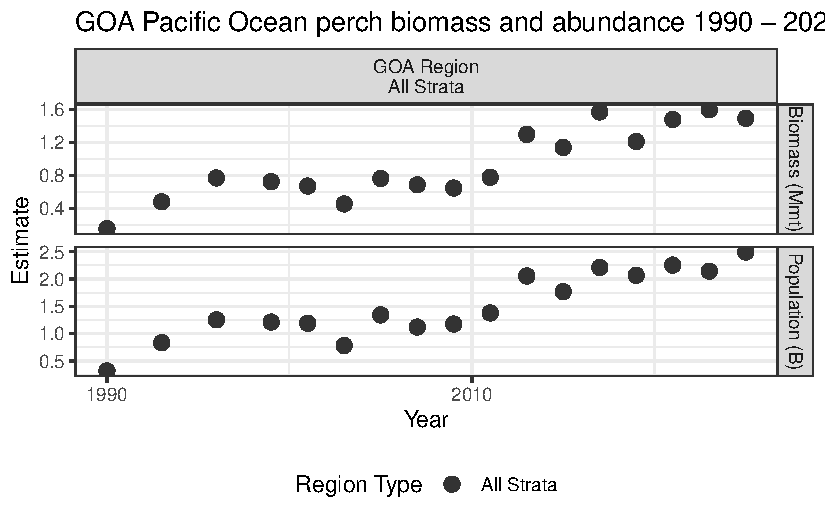
\includegraphics{content/akfin-oracle-sql-r_files/figure-pdf/test-1-plot-1.pdf}

}

\caption{Ex. 1: GOA Pacific Ocean perch biomass and abundance.}

\end{figure}

\hypertarget{ex.-2-ai-rock-sole-size-compositions-and-ridge-plot}{%
\subsection{Ex. 2: AI Rock sole size compositions and ridge
plot}\label{ex.-2-ai-rock-sole-size-compositions-and-ridge-plot}}

Northern and Southern rock sole size composition data from 1991 -- 2022
for the Aleutian Islands, with Ridge plot from
\href{https://cran.r-project.org/web/packages/ggridges/vignettes/introduction.html}{\texttt{ggridges}}.

\begin{Shaded}
\begin{Highlighting}[]
\NormalTok{dat }\OtherTok{\textless{}{-}}\NormalTok{ RODBC}\SpecialCharTok{::}\FunctionTok{sqlQuery}\NormalTok{(}\AttributeTok{channel =}\NormalTok{ channel, }
                       \AttributeTok{query =} 
\StringTok{"WITH FILTERED\_STRATA AS (}
\StringTok{SELECT }
\StringTok{AREA\_ID, }
\StringTok{DESCRIPTION }
\StringTok{FROM GAP\_PRODUCTS.AKFIN\_AREA}
\StringTok{WHERE TYPE = \textquotesingle{}REGION\textquotesingle{} }
\StringTok{AND SURVEY\_DEFINITION\_ID = 52)}
\StringTok{SELECT }
\StringTok{LENGTH\_MM, }
\StringTok{YEAR}
\StringTok{FROM GAP\_PRODUCTS.AKFIN\_SIZECOMP SIZECOMP}
\StringTok{JOIN FILTERED\_STRATA STRATA }
\StringTok{ON STRATA.AREA\_ID = SIZECOMP.AREA\_ID}
\StringTok{WHERE SIZECOMP.SURVEY\_DEFINITION\_ID IN 52 }
\StringTok{AND SIZECOMP.SPECIES\_CODE IN (10261, 10262)"}\NormalTok{)}
\end{Highlighting}
\end{Shaded}

\begin{Shaded}
\begin{Highlighting}[]
\NormalTok{dat0 }\OtherTok{\textless{}{-}}\NormalTok{ dat }\SpecialCharTok{\%\textgreater{}\%} 
\NormalTok{  janitor}\SpecialCharTok{::}\FunctionTok{clean\_names}\NormalTok{() }\SpecialCharTok{\%\textgreater{}\%} 
\NormalTok{  dplyr}\SpecialCharTok{::}\FunctionTok{mutate}\NormalTok{(}\AttributeTok{length\_cm =}\NormalTok{ length\_mm}\SpecialCharTok{/}\DecValTok{10}\NormalTok{)}
\NormalTok{flextable}\SpecialCharTok{::}\FunctionTok{flextable}\NormalTok{(}\FunctionTok{head}\NormalTok{(dat)) }\SpecialCharTok{\%\textgreater{}\%} 
  \FunctionTok{theme\_zebra}\NormalTok{() }\SpecialCharTok{\%\textgreater{}\%}
\NormalTok{    flextable}\SpecialCharTok{::}\FunctionTok{colformat\_num}\NormalTok{(}\AttributeTok{x =}\NormalTok{ ., }\AttributeTok{j =} \StringTok{"YEAR"}\NormalTok{, }\AttributeTok{big.mark =} \StringTok{""}\NormalTok{)}
\end{Highlighting}
\end{Shaded}

\global\setlength{\Oldarrayrulewidth}{\arrayrulewidth}

\global\setlength{\Oldtabcolsep}{\tabcolsep}

\setlength{\tabcolsep}{0pt}

\renewcommand*{\arraystretch}{1.5}



\providecommand{\ascline}[3]{\noalign{\global\arrayrulewidth #1}\arrayrulecolor[HTML]{#2}\cline{#3}}

\begin{longtable}[c]{|p{0.75in}|p{0.75in}}
\caption{Ex. 2: AI Rock sole size compositions and ridge plot.}\tabularnewline




\hhline{>{\arrayrulecolor[HTML]{000000}\global\arrayrulewidth=0pt}->{\arrayrulecolor[HTML]{000000}\global\arrayrulewidth=0pt}-}

\multicolumn{1}{>{\cellcolor[HTML]{CFCFCF}\raggedleft}m{\dimexpr 0.75in+0\tabcolsep}}{\textcolor[HTML]{000000}{\fontsize{11}{11}\selectfont{\textbf{LENGTH\_MM}}}} & \multicolumn{1}{>{\cellcolor[HTML]{CFCFCF}\raggedleft}m{\dimexpr 0.75in+0\tabcolsep}}{\textcolor[HTML]{000000}{\fontsize{11}{11}\selectfont{\textbf{YEAR}}}} \\

\noalign{\global\arrayrulewidth 0pt}\arrayrulecolor[HTML]{000000}

\endfirsthead 

\hhline{>{\arrayrulecolor[HTML]{000000}\global\arrayrulewidth=0pt}->{\arrayrulecolor[HTML]{000000}\global\arrayrulewidth=0pt}-}

\multicolumn{1}{>{\cellcolor[HTML]{CFCFCF}\raggedleft}m{\dimexpr 0.75in+0\tabcolsep}}{\textcolor[HTML]{000000}{\fontsize{11}{11}\selectfont{\textbf{LENGTH\_MM}}}} & \multicolumn{1}{>{\cellcolor[HTML]{CFCFCF}\raggedleft}m{\dimexpr 0.75in+0\tabcolsep}}{\textcolor[HTML]{000000}{\fontsize{11}{11}\selectfont{\textbf{YEAR}}}} \\

\noalign{\global\arrayrulewidth 0pt}\arrayrulecolor[HTML]{000000}

\endhead



\multicolumn{1}{>{\cellcolor[HTML]{EFEFEF}\raggedleft}m{\dimexpr 0.75in+0\tabcolsep}}{\textcolor[HTML]{000000}{\fontsize{11}{11}\selectfont{180}}} & \multicolumn{1}{>{\cellcolor[HTML]{EFEFEF}\raggedleft}m{\dimexpr 0.75in+0\tabcolsep}}{\textcolor[HTML]{000000}{\fontsize{11}{11}\selectfont{2014}}} \\

\noalign{\global\arrayrulewidth 0pt}\arrayrulecolor[HTML]{000000}





\multicolumn{1}{>{\raggedleft}m{\dimexpr 0.75in+0\tabcolsep}}{\textcolor[HTML]{000000}{\fontsize{11}{11}\selectfont{190}}} & \multicolumn{1}{>{\raggedleft}m{\dimexpr 0.75in+0\tabcolsep}}{\textcolor[HTML]{000000}{\fontsize{11}{11}\selectfont{2014}}} \\

\noalign{\global\arrayrulewidth 0pt}\arrayrulecolor[HTML]{000000}





\multicolumn{1}{>{\cellcolor[HTML]{EFEFEF}\raggedleft}m{\dimexpr 0.75in+0\tabcolsep}}{\textcolor[HTML]{000000}{\fontsize{11}{11}\selectfont{200}}} & \multicolumn{1}{>{\cellcolor[HTML]{EFEFEF}\raggedleft}m{\dimexpr 0.75in+0\tabcolsep}}{\textcolor[HTML]{000000}{\fontsize{11}{11}\selectfont{2014}}} \\

\noalign{\global\arrayrulewidth 0pt}\arrayrulecolor[HTML]{000000}





\multicolumn{1}{>{\raggedleft}m{\dimexpr 0.75in+0\tabcolsep}}{\textcolor[HTML]{000000}{\fontsize{11}{11}\selectfont{210}}} & \multicolumn{1}{>{\raggedleft}m{\dimexpr 0.75in+0\tabcolsep}}{\textcolor[HTML]{000000}{\fontsize{11}{11}\selectfont{2014}}} \\

\noalign{\global\arrayrulewidth 0pt}\arrayrulecolor[HTML]{000000}





\multicolumn{1}{>{\cellcolor[HTML]{EFEFEF}\raggedleft}m{\dimexpr 0.75in+0\tabcolsep}}{\textcolor[HTML]{000000}{\fontsize{11}{11}\selectfont{220}}} & \multicolumn{1}{>{\cellcolor[HTML]{EFEFEF}\raggedleft}m{\dimexpr 0.75in+0\tabcolsep}}{\textcolor[HTML]{000000}{\fontsize{11}{11}\selectfont{2014}}} \\

\noalign{\global\arrayrulewidth 0pt}\arrayrulecolor[HTML]{000000}





\multicolumn{1}{>{\raggedleft}m{\dimexpr 0.75in+0\tabcolsep}}{\textcolor[HTML]{000000}{\fontsize{11}{11}\selectfont{230}}} & \multicolumn{1}{>{\raggedleft}m{\dimexpr 0.75in+0\tabcolsep}}{\textcolor[HTML]{000000}{\fontsize{11}{11}\selectfont{2014}}} \\

\noalign{\global\arrayrulewidth 0pt}\arrayrulecolor[HTML]{000000}





\end{longtable}



\arrayrulecolor[HTML]{000000}

\global\setlength{\arrayrulewidth}{\Oldarrayrulewidth}

\global\setlength{\tabcolsep}{\Oldtabcolsep}

\renewcommand*{\arraystretch}{1}

\begin{Shaded}
\begin{Highlighting}[]
\CommentTok{\# install.packages("ggridges")}
\FunctionTok{library}\NormalTok{(ggridges)}
\NormalTok{figure }\OtherTok{\textless{}{-}} 
\NormalTok{  ggplot2}\SpecialCharTok{::}\FunctionTok{ggplot}\NormalTok{(}
    \AttributeTok{data =}\NormalTok{ dat0, }
    \AttributeTok{mapping =} \FunctionTok{aes}\NormalTok{(}\AttributeTok{x =}\NormalTok{ length\_cm, }\AttributeTok{y =} \FunctionTok{as.factor}\NormalTok{(year), }\AttributeTok{fill =} \FunctionTok{stat}\NormalTok{(x))) }\SpecialCharTok{+}
\NormalTok{  ggridges}\SpecialCharTok{::}\FunctionTok{theme\_ridges}\NormalTok{(}\AttributeTok{center\_axis\_labels =} \ConstantTok{TRUE}\NormalTok{) }\SpecialCharTok{+} 
\NormalTok{  ggridges}\SpecialCharTok{::}\FunctionTok{geom\_density\_ridges\_gradient}\NormalTok{(}\AttributeTok{scale =} \DecValTok{4}\NormalTok{, }\AttributeTok{show.legend =} \ConstantTok{FALSE}\NormalTok{) }\SpecialCharTok{+} 
\NormalTok{  ggplot2}\SpecialCharTok{::}\FunctionTok{scale\_y\_discrete}\NormalTok{(}\AttributeTok{name =} \StringTok{"Year"}\NormalTok{, }\AttributeTok{expand =} \FunctionTok{c}\NormalTok{(}\FloatTok{0.01}\NormalTok{, }\DecValTok{0}\NormalTok{)) }\SpecialCharTok{+}
\NormalTok{  ggplot2}\SpecialCharTok{::}\FunctionTok{scale\_x\_continuous}\NormalTok{(}\AttributeTok{name =} \StringTok{"Length (cm)"}\NormalTok{, }\AttributeTok{expand =} \FunctionTok{c}\NormalTok{(}\FloatTok{0.01}\NormalTok{, }\DecValTok{0}\NormalTok{)) }\SpecialCharTok{+}
  \CommentTok{\# ggplot2::scale\_fill\_grey() +}
\NormalTok{  ggplot2}\SpecialCharTok{::}\FunctionTok{labs}\NormalTok{(}\AttributeTok{title =} \StringTok{\textquotesingle{}AI Rock sole Size Compositions 1991 – 2022\textquotesingle{}}\NormalTok{) }

\NormalTok{figure}
\end{Highlighting}
\end{Shaded}

\begin{figure}[H]

{\centering 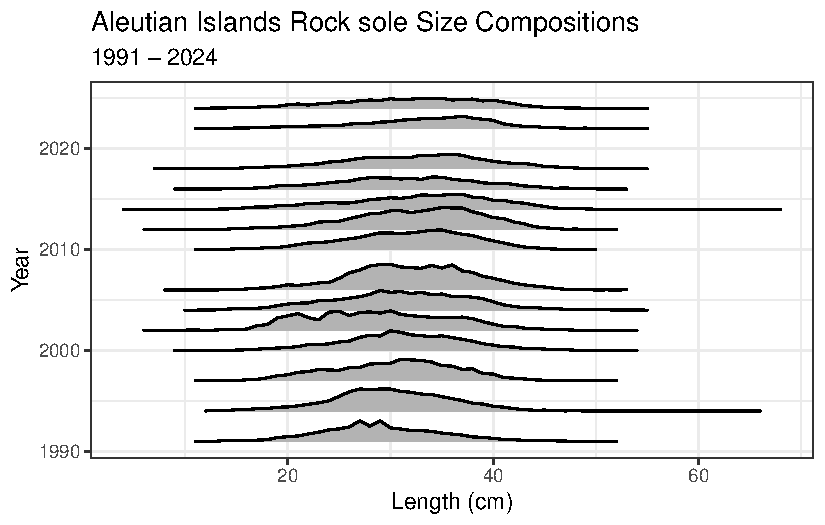
\includegraphics{content/akfin-oracle-sql-r_files/figure-pdf/test-2-plot-1.pdf}

}

\caption{Ex. 2: AI Rock sole size compositions and ridge plot.}

\end{figure}

\hypertarget{ex.-3-ebs-walleye-pollock-age-compositions-and-age-pyramid}{%
\subsection{Ex. 3: EBS Walleye Pollock Age Compositions and Age
Pyramid}\label{ex.-3-ebs-walleye-pollock-age-compositions-and-age-pyramid}}

Walleye pollock age composition for the EBS Standard Area from 1982 --
2022 and the EBS + NW Area from 1987 -- 2022, with age pyramid plot.

\begin{Shaded}
\begin{Highlighting}[]
\NormalTok{dat }\OtherTok{\textless{}{-}}\NormalTok{ RODBC}\SpecialCharTok{::}\FunctionTok{sqlQuery}\NormalTok{(}\AttributeTok{channel =}\NormalTok{ channel, }
                       \AttributeTok{query =} 
\StringTok{"WITH FILTERED\_STRATA AS (}
\StringTok{SELECT }
\StringTok{AREA\_ID, }
\StringTok{DESCRIPTION }
\StringTok{FROM GAP\_PRODUCTS.AKFIN\_AREA}
\StringTok{WHERE TYPE = \textquotesingle{}REGION\textquotesingle{} AND }
\StringTok{SURVEY\_DEFINITION\_ID = 98)}
\StringTok{SELECT }
\StringTok{AGECOMP.AGE, }
\StringTok{AGECOMP.POPULATION\_COUNT, }
\StringTok{AGECOMP.SEX}
\StringTok{FROM GAP\_PRODUCTS.AKFIN\_AGECOMP AGECOMP}
\StringTok{JOIN FILTERED\_STRATA STRATA }
\StringTok{ON STRATA.AREA\_ID = AGECOMP.AREA\_ID}
\StringTok{WHERE SURVEY\_DEFINITION\_ID = 98 }
\StringTok{AND SPECIES\_CODE = 21740}
\StringTok{AND AGE \textgreater{}= 0"}\NormalTok{)}
\end{Highlighting}
\end{Shaded}

\begin{Shaded}
\begin{Highlighting}[]
\NormalTok{dat0 }\OtherTok{\textless{}{-}}\NormalTok{ dat }\SpecialCharTok{\%\textgreater{}\%} 
\NormalTok{  janitor}\SpecialCharTok{::}\FunctionTok{clean\_names}\NormalTok{() }\SpecialCharTok{\%\textgreater{}\%} 
\NormalTok{  dplyr}\SpecialCharTok{::}\FunctionTok{filter}\NormalTok{(sex }\SpecialCharTok{\%in\%} \FunctionTok{c}\NormalTok{(}\DecValTok{1}\NormalTok{,}\DecValTok{2}\NormalTok{)) }\SpecialCharTok{\%\textgreater{}\%}
\NormalTok{  dplyr}\SpecialCharTok{::}\FunctionTok{mutate}\NormalTok{(}
    \AttributeTok{sex =} \FunctionTok{ifelse}\NormalTok{(sex }\SpecialCharTok{==} \DecValTok{1}\NormalTok{, }\StringTok{"M"}\NormalTok{, }\StringTok{"F"}\NormalTok{),}
    \AttributeTok{population\_count =} \CommentTok{\# change male population to negative}
      \FunctionTok{ifelse}\NormalTok{(sex}\SpecialCharTok{==}\StringTok{"M"}\NormalTok{, population\_count}\SpecialCharTok{*}\NormalTok{(}\SpecialCharTok{{-}}\DecValTok{1}\NormalTok{), population\_count}\SpecialCharTok{*}\DecValTok{1}\NormalTok{)}\SpecialCharTok{/}\FloatTok{1e9}\NormalTok{) }

\NormalTok{flextable}\SpecialCharTok{::}\FunctionTok{flextable}\NormalTok{(}\FunctionTok{head}\NormalTok{(dat)) }\SpecialCharTok{\%\textgreater{}\%} \FunctionTok{theme\_zebra}\NormalTok{()}
\end{Highlighting}
\end{Shaded}

\global\setlength{\Oldarrayrulewidth}{\arrayrulewidth}

\global\setlength{\Oldtabcolsep}{\tabcolsep}

\setlength{\tabcolsep}{0pt}

\renewcommand*{\arraystretch}{1.5}



\providecommand{\ascline}[3]{\noalign{\global\arrayrulewidth #1}\arrayrulecolor[HTML]{#2}\cline{#3}}

\begin{longtable}[c]{|p{0.75in}|p{0.75in}|p{0.75in}}
\caption{Ex. 3: EBS Walleye Pollock Age Compositions and Age Pyramid.}\tabularnewline




\hhline{>{\arrayrulecolor[HTML]{000000}\global\arrayrulewidth=0pt}->{\arrayrulecolor[HTML]{000000}\global\arrayrulewidth=0pt}->{\arrayrulecolor[HTML]{000000}\global\arrayrulewidth=0pt}-}

\multicolumn{1}{>{\cellcolor[HTML]{CFCFCF}\raggedleft}m{\dimexpr 0.75in+0\tabcolsep}}{\textcolor[HTML]{000000}{\fontsize{11}{11}\selectfont{\textbf{AGE}}}} & \multicolumn{1}{>{\cellcolor[HTML]{CFCFCF}\raggedleft}m{\dimexpr 0.75in+0\tabcolsep}}{\textcolor[HTML]{000000}{\fontsize{11}{11}\selectfont{\textbf{POPULATION\_COUNT}}}} & \multicolumn{1}{>{\cellcolor[HTML]{CFCFCF}\raggedleft}m{\dimexpr 0.75in+0\tabcolsep}}{\textcolor[HTML]{000000}{\fontsize{11}{11}\selectfont{\textbf{SEX}}}} \\

\noalign{\global\arrayrulewidth 0pt}\arrayrulecolor[HTML]{000000}

\endfirsthead 

\hhline{>{\arrayrulecolor[HTML]{000000}\global\arrayrulewidth=0pt}->{\arrayrulecolor[HTML]{000000}\global\arrayrulewidth=0pt}->{\arrayrulecolor[HTML]{000000}\global\arrayrulewidth=0pt}-}

\multicolumn{1}{>{\cellcolor[HTML]{CFCFCF}\raggedleft}m{\dimexpr 0.75in+0\tabcolsep}}{\textcolor[HTML]{000000}{\fontsize{11}{11}\selectfont{\textbf{AGE}}}} & \multicolumn{1}{>{\cellcolor[HTML]{CFCFCF}\raggedleft}m{\dimexpr 0.75in+0\tabcolsep}}{\textcolor[HTML]{000000}{\fontsize{11}{11}\selectfont{\textbf{POPULATION\_COUNT}}}} & \multicolumn{1}{>{\cellcolor[HTML]{CFCFCF}\raggedleft}m{\dimexpr 0.75in+0\tabcolsep}}{\textcolor[HTML]{000000}{\fontsize{11}{11}\selectfont{\textbf{SEX}}}} \\

\noalign{\global\arrayrulewidth 0pt}\arrayrulecolor[HTML]{000000}

\endhead



\multicolumn{1}{>{\cellcolor[HTML]{EFEFEF}\raggedleft}m{\dimexpr 0.75in+0\tabcolsep}}{\textcolor[HTML]{000000}{\fontsize{11}{11}\selectfont{9}}} & \multicolumn{1}{>{\cellcolor[HTML]{EFEFEF}\raggedleft}m{\dimexpr 0.75in+0\tabcolsep}}{\textcolor[HTML]{000000}{\fontsize{11}{11}\selectfont{39,371}}} & \multicolumn{1}{>{\cellcolor[HTML]{EFEFEF}\raggedleft}m{\dimexpr 0.75in+0\tabcolsep}}{\textcolor[HTML]{000000}{\fontsize{11}{11}\selectfont{3}}} \\

\noalign{\global\arrayrulewidth 0pt}\arrayrulecolor[HTML]{000000}





\multicolumn{1}{>{\raggedleft}m{\dimexpr 0.75in+0\tabcolsep}}{\textcolor[HTML]{000000}{\fontsize{11}{11}\selectfont{10}}} & \multicolumn{1}{>{\raggedleft}m{\dimexpr 0.75in+0\tabcolsep}}{\textcolor[HTML]{000000}{\fontsize{11}{11}\selectfont{32,156}}} & \multicolumn{1}{>{\raggedleft}m{\dimexpr 0.75in+0\tabcolsep}}{\textcolor[HTML]{000000}{\fontsize{11}{11}\selectfont{3}}} \\

\noalign{\global\arrayrulewidth 0pt}\arrayrulecolor[HTML]{000000}





\multicolumn{1}{>{\cellcolor[HTML]{EFEFEF}\raggedleft}m{\dimexpr 0.75in+0\tabcolsep}}{\textcolor[HTML]{000000}{\fontsize{11}{11}\selectfont{11}}} & \multicolumn{1}{>{\cellcolor[HTML]{EFEFEF}\raggedleft}m{\dimexpr 0.75in+0\tabcolsep}}{\textcolor[HTML]{000000}{\fontsize{11}{11}\selectfont{15,200}}} & \multicolumn{1}{>{\cellcolor[HTML]{EFEFEF}\raggedleft}m{\dimexpr 0.75in+0\tabcolsep}}{\textcolor[HTML]{000000}{\fontsize{11}{11}\selectfont{3}}} \\

\noalign{\global\arrayrulewidth 0pt}\arrayrulecolor[HTML]{000000}





\multicolumn{1}{>{\raggedleft}m{\dimexpr 0.75in+0\tabcolsep}}{\textcolor[HTML]{000000}{\fontsize{11}{11}\selectfont{12}}} & \multicolumn{1}{>{\raggedleft}m{\dimexpr 0.75in+0\tabcolsep}}{\textcolor[HTML]{000000}{\fontsize{11}{11}\selectfont{9,976}}} & \multicolumn{1}{>{\raggedleft}m{\dimexpr 0.75in+0\tabcolsep}}{\textcolor[HTML]{000000}{\fontsize{11}{11}\selectfont{3}}} \\

\noalign{\global\arrayrulewidth 0pt}\arrayrulecolor[HTML]{000000}





\multicolumn{1}{>{\cellcolor[HTML]{EFEFEF}\raggedleft}m{\dimexpr 0.75in+0\tabcolsep}}{\textcolor[HTML]{000000}{\fontsize{11}{11}\selectfont{13}}} & \multicolumn{1}{>{\cellcolor[HTML]{EFEFEF}\raggedleft}m{\dimexpr 0.75in+0\tabcolsep}}{\textcolor[HTML]{000000}{\fontsize{11}{11}\selectfont{1,957}}} & \multicolumn{1}{>{\cellcolor[HTML]{EFEFEF}\raggedleft}m{\dimexpr 0.75in+0\tabcolsep}}{\textcolor[HTML]{000000}{\fontsize{11}{11}\selectfont{3}}} \\

\noalign{\global\arrayrulewidth 0pt}\arrayrulecolor[HTML]{000000}





\multicolumn{1}{>{\raggedleft}m{\dimexpr 0.75in+0\tabcolsep}}{\textcolor[HTML]{000000}{\fontsize{11}{11}\selectfont{1}}} & \multicolumn{1}{>{\raggedleft}m{\dimexpr 0.75in+0\tabcolsep}}{\textcolor[HTML]{000000}{\fontsize{11}{11}\selectfont{131,950,343}}} & \multicolumn{1}{>{\raggedleft}m{\dimexpr 0.75in+0\tabcolsep}}{\textcolor[HTML]{000000}{\fontsize{11}{11}\selectfont{1}}} \\

\noalign{\global\arrayrulewidth 0pt}\arrayrulecolor[HTML]{000000}





\end{longtable}



\arrayrulecolor[HTML]{000000}

\global\setlength{\arrayrulewidth}{\Oldarrayrulewidth}

\global\setlength{\tabcolsep}{\Oldtabcolsep}

\renewcommand*{\arraystretch}{1}

\begin{Shaded}
\begin{Highlighting}[]
\NormalTok{figure }\OtherTok{\textless{}{-}}\NormalTok{ ggplot2}\SpecialCharTok{::}\FunctionTok{ggplot}\NormalTok{(}
  \AttributeTok{data =}\NormalTok{ dat0, }
  \AttributeTok{mapping =} 
                 \FunctionTok{aes}\NormalTok{(}\AttributeTok{x =}\NormalTok{ age,}
                     \AttributeTok{y =}\NormalTok{ population\_count, }
                     \AttributeTok{fill =}\NormalTok{ sex)) }\SpecialCharTok{+}
\NormalTok{  ggplot2}\SpecialCharTok{::}\FunctionTok{scale\_fill\_grey}\NormalTok{() }\SpecialCharTok{+}
\NormalTok{  ggplot2}\SpecialCharTok{::}\FunctionTok{geom\_bar}\NormalTok{(}\AttributeTok{stat =} \StringTok{"identity"}\NormalTok{) }\SpecialCharTok{+}
\NormalTok{  ggplot2}\SpecialCharTok{::}\FunctionTok{coord\_flip}\NormalTok{() }\SpecialCharTok{+}
\NormalTok{  ggplot2}\SpecialCharTok{::}\FunctionTok{scale\_x\_continuous}\NormalTok{(}\AttributeTok{name =} \StringTok{"Age"}\NormalTok{) }\SpecialCharTok{+}
\NormalTok{  ggplot2}\SpecialCharTok{::}\FunctionTok{scale\_y\_continuous}\NormalTok{(}\AttributeTok{name =} \StringTok{"Population (billions)"}\NormalTok{, }\AttributeTok{labels =}\NormalTok{ abs) }\SpecialCharTok{+}
\NormalTok{  ggplot2}\SpecialCharTok{::}\FunctionTok{ggtitle}\NormalTok{(}\AttributeTok{label =} \StringTok{"EBS Walleye Pollock Age Compositions 1982 – 2022"}\NormalTok{)  }\SpecialCharTok{+} 
\NormalTok{  ggplot2}\SpecialCharTok{::}\FunctionTok{guides}\NormalTok{(}\AttributeTok{fill =} \FunctionTok{guide\_legend}\NormalTok{(}\AttributeTok{title =} \StringTok{"Sex"}\NormalTok{))}\SpecialCharTok{+}
\NormalTok{  ggplot2}\SpecialCharTok{::}\FunctionTok{theme\_bw}\NormalTok{()}

\NormalTok{figure}
\end{Highlighting}
\end{Shaded}

\begin{figure}[H]

{\centering 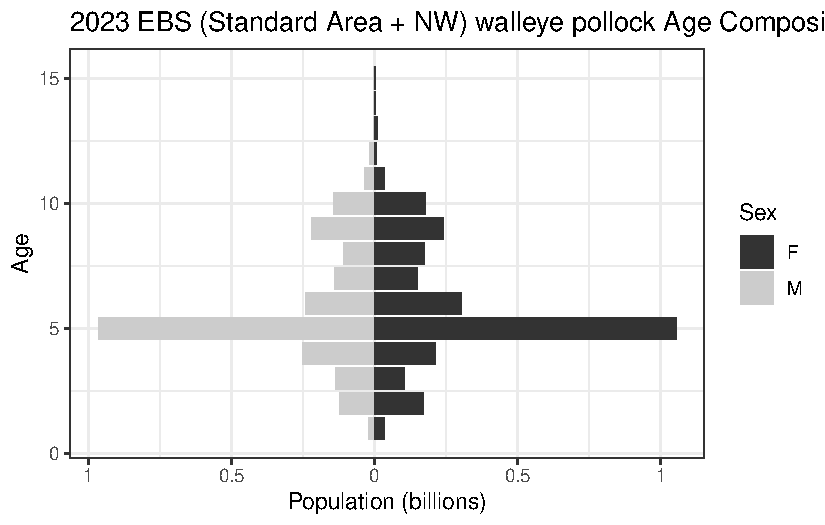
\includegraphics{content/akfin-oracle-sql-r_files/figure-pdf/test-3-plot-1.pdf}

}

\caption{Ex. 3: EBS Walleye Pollock Age Compositions and Age Pyramid.}

\end{figure}

\hypertarget{ex.-4-nbs-pacific-cod-biomass-and-abundance}{%
\subsection{Ex. 4: NBS Pacific cod biomass and
abundance}\label{ex.-4-nbs-pacific-cod-biomass-and-abundance}}

Pacific cod biomass and abundance data for the NBS by stratum.

\begin{Shaded}
\begin{Highlighting}[]
\NormalTok{dat }\OtherTok{\textless{}{-}}\NormalTok{ RODBC}\SpecialCharTok{::}\FunctionTok{sqlQuery}\NormalTok{(}\AttributeTok{channel =}\NormalTok{ channel, }
                       \AttributeTok{query =} 
\StringTok{"WITH FILTERED\_STRATA AS (}
\StringTok{SELECT }
\StringTok{AREA\_ID, }
\StringTok{AREA\_NAME, }
\StringTok{DESCRIPTION }
\StringTok{FROM GAP\_PRODUCTS.AKFIN\_AREA}
\StringTok{WHERE TYPE in (\textquotesingle{}STRATUM\textquotesingle{}) AND }
\StringTok{SURVEY\_DEFINITION\_ID = 143) }
\StringTok{SELECT }
\StringTok{BIOMASS.BIOMASS\_MT, }
\StringTok{BIOMASS.POPULATION\_COUNT, }
\StringTok{BIOMASS.YEAR, }
\StringTok{STRATA.AREA\_NAME}
\StringTok{FROM GAP\_PRODUCTS.AKFIN\_BIOMASS BIOMASS }
\StringTok{JOIN FILTERED\_STRATA STRATA }
\StringTok{ON STRATA.AREA\_ID = BIOMASS.AREA\_ID}
\StringTok{WHERE BIOMASS.SURVEY\_DEFINITION\_ID IN 143 }
\StringTok{AND BIOMASS.SPECIES\_CODE = 21720"}\NormalTok{)}
\end{Highlighting}
\end{Shaded}

\begin{Shaded}
\begin{Highlighting}[]
\NormalTok{dat0 }\OtherTok{\textless{}{-}}\NormalTok{ dat }\SpecialCharTok{\%\textgreater{}\%} 
\NormalTok{  janitor}\SpecialCharTok{::}\FunctionTok{clean\_names}\NormalTok{() }\SpecialCharTok{\%\textgreater{}\%} 
\NormalTok{  dplyr}\SpecialCharTok{::}\FunctionTok{select}\NormalTok{(biomass\_mt, population\_count, year, }\AttributeTok{area =}\NormalTok{ area\_name) }\SpecialCharTok{\%\textgreater{}\%}
  \FunctionTok{pivot\_longer}\NormalTok{(}\AttributeTok{cols =} \FunctionTok{c}\NormalTok{(}\StringTok{"biomass\_mt"}\NormalTok{, }\StringTok{"population\_count"}\NormalTok{), }
               \AttributeTok{names\_to =} \StringTok{"var"}\NormalTok{, }
               \AttributeTok{values\_to =} \StringTok{"val"}\NormalTok{) }\SpecialCharTok{\%\textgreater{}\%} 
\NormalTok{  dplyr}\SpecialCharTok{::}\FunctionTok{mutate}\NormalTok{(}
    \AttributeTok{val =} \FunctionTok{ifelse}\NormalTok{(var }\SpecialCharTok{==} \StringTok{"biomass\_mt"}\NormalTok{, val}\SpecialCharTok{/}\FloatTok{1e6}\NormalTok{, val}\SpecialCharTok{/}\FloatTok{1e9}\NormalTok{), }
    \AttributeTok{var =} \FunctionTok{ifelse}\NormalTok{(var }\SpecialCharTok{==} \StringTok{"biomass\_mt"}\NormalTok{, }\StringTok{"Biomass (Mmt)"}\NormalTok{, }\StringTok{"Population (B)"}\NormalTok{), }
    \AttributeTok{area =} \FunctionTok{factor}\NormalTok{(area, }\AttributeTok{levels =} \FunctionTok{unique}\NormalTok{(area), }\AttributeTok{labels =} \FunctionTok{unique}\NormalTok{(area), }\AttributeTok{ordered =} \ConstantTok{TRUE}\NormalTok{))}
\NormalTok{flextable}\SpecialCharTok{::}\FunctionTok{flextable}\NormalTok{(}\FunctionTok{head}\NormalTok{(dat)) }\SpecialCharTok{\%\textgreater{}\%} 
  \FunctionTok{theme\_zebra}\NormalTok{() }\SpecialCharTok{\%\textgreater{}\%}
\NormalTok{  flextable}\SpecialCharTok{::}\FunctionTok{colformat\_num}\NormalTok{(}\AttributeTok{x =}\NormalTok{ ., }\AttributeTok{j =} \StringTok{"YEAR"}\NormalTok{, }\AttributeTok{big.mark =} \StringTok{""}\NormalTok{)}
\end{Highlighting}
\end{Shaded}

\global\setlength{\Oldarrayrulewidth}{\arrayrulewidth}

\global\setlength{\Oldtabcolsep}{\tabcolsep}

\setlength{\tabcolsep}{0pt}

\renewcommand*{\arraystretch}{1.5}



\providecommand{\ascline}[3]{\noalign{\global\arrayrulewidth #1}\arrayrulecolor[HTML]{#2}\cline{#3}}

\begin{longtable}[c]{|p{0.75in}|p{0.75in}|p{0.75in}|p{0.75in}}
\caption{Ex. 4: NBS Pacific cod biomass and abundance.}\tabularnewline




\hhline{>{\arrayrulecolor[HTML]{000000}\global\arrayrulewidth=0pt}->{\arrayrulecolor[HTML]{000000}\global\arrayrulewidth=0pt}->{\arrayrulecolor[HTML]{000000}\global\arrayrulewidth=0pt}->{\arrayrulecolor[HTML]{000000}\global\arrayrulewidth=0pt}-}

\multicolumn{1}{>{\cellcolor[HTML]{CFCFCF}\raggedleft}m{\dimexpr 0.75in+0\tabcolsep}}{\textcolor[HTML]{000000}{\fontsize{11}{11}\selectfont{\textbf{BIOMASS\_MT}}}} & \multicolumn{1}{>{\cellcolor[HTML]{CFCFCF}\raggedleft}m{\dimexpr 0.75in+0\tabcolsep}}{\textcolor[HTML]{000000}{\fontsize{11}{11}\selectfont{\textbf{POPULATION\_COUNT}}}} & \multicolumn{1}{>{\cellcolor[HTML]{CFCFCF}\raggedleft}m{\dimexpr 0.75in+0\tabcolsep}}{\textcolor[HTML]{000000}{\fontsize{11}{11}\selectfont{\textbf{YEAR}}}} & \multicolumn{1}{>{\cellcolor[HTML]{CFCFCF}\raggedright}m{\dimexpr 0.75in+0\tabcolsep}}{\textcolor[HTML]{000000}{\fontsize{11}{11}\selectfont{\textbf{AREA\_NAME}}}} \\

\noalign{\global\arrayrulewidth 0pt}\arrayrulecolor[HTML]{000000}

\endfirsthead 

\hhline{>{\arrayrulecolor[HTML]{000000}\global\arrayrulewidth=0pt}->{\arrayrulecolor[HTML]{000000}\global\arrayrulewidth=0pt}->{\arrayrulecolor[HTML]{000000}\global\arrayrulewidth=0pt}->{\arrayrulecolor[HTML]{000000}\global\arrayrulewidth=0pt}-}

\multicolumn{1}{>{\cellcolor[HTML]{CFCFCF}\raggedleft}m{\dimexpr 0.75in+0\tabcolsep}}{\textcolor[HTML]{000000}{\fontsize{11}{11}\selectfont{\textbf{BIOMASS\_MT}}}} & \multicolumn{1}{>{\cellcolor[HTML]{CFCFCF}\raggedleft}m{\dimexpr 0.75in+0\tabcolsep}}{\textcolor[HTML]{000000}{\fontsize{11}{11}\selectfont{\textbf{POPULATION\_COUNT}}}} & \multicolumn{1}{>{\cellcolor[HTML]{CFCFCF}\raggedleft}m{\dimexpr 0.75in+0\tabcolsep}}{\textcolor[HTML]{000000}{\fontsize{11}{11}\selectfont{\textbf{YEAR}}}} & \multicolumn{1}{>{\cellcolor[HTML]{CFCFCF}\raggedright}m{\dimexpr 0.75in+0\tabcolsep}}{\textcolor[HTML]{000000}{\fontsize{11}{11}\selectfont{\textbf{AREA\_NAME}}}} \\

\noalign{\global\arrayrulewidth 0pt}\arrayrulecolor[HTML]{000000}

\endhead



\multicolumn{1}{>{\cellcolor[HTML]{EFEFEF}\raggedleft}m{\dimexpr 0.75in+0\tabcolsep}}{\textcolor[HTML]{000000}{\fontsize{11}{11}\selectfont{26,747.07}}} & \multicolumn{1}{>{\cellcolor[HTML]{EFEFEF}\raggedleft}m{\dimexpr 0.75in+0\tabcolsep}}{\textcolor[HTML]{000000}{\fontsize{11}{11}\selectfont{10,447,602}}} & \multicolumn{1}{>{\cellcolor[HTML]{EFEFEF}\raggedleft}m{\dimexpr 0.75in+0\tabcolsep}}{\textcolor[HTML]{000000}{\fontsize{11}{11}\selectfont{2022}}} & \multicolumn{1}{>{\cellcolor[HTML]{EFEFEF}\raggedright}m{\dimexpr 0.75in+0\tabcolsep}}{\textcolor[HTML]{000000}{\fontsize{11}{11}\selectfont{Inner\ Domain}}} \\

\noalign{\global\arrayrulewidth 0pt}\arrayrulecolor[HTML]{000000}





\multicolumn{1}{>{\raggedleft}m{\dimexpr 0.75in+0\tabcolsep}}{\textcolor[HTML]{000000}{\fontsize{11}{11}\selectfont{26,747.07}}} & \multicolumn{1}{>{\raggedleft}m{\dimexpr 0.75in+0\tabcolsep}}{\textcolor[HTML]{000000}{\fontsize{11}{11}\selectfont{10,447,602}}} & \multicolumn{1}{>{\raggedleft}m{\dimexpr 0.75in+0\tabcolsep}}{\textcolor[HTML]{000000}{\fontsize{11}{11}\selectfont{2022}}} & \multicolumn{1}{>{\raggedright}m{\dimexpr 0.75in+0\tabcolsep}}{\textcolor[HTML]{000000}{\fontsize{11}{11}\selectfont{Inner\ Domain}}} \\

\noalign{\global\arrayrulewidth 0pt}\arrayrulecolor[HTML]{000000}





\multicolumn{1}{>{\cellcolor[HTML]{EFEFEF}\raggedleft}m{\dimexpr 0.75in+0\tabcolsep}}{\textcolor[HTML]{000000}{\fontsize{11}{11}\selectfont{95,849.98}}} & \multicolumn{1}{>{\cellcolor[HTML]{EFEFEF}\raggedleft}m{\dimexpr 0.75in+0\tabcolsep}}{\textcolor[HTML]{000000}{\fontsize{11}{11}\selectfont{68,767,498}}} & \multicolumn{1}{>{\cellcolor[HTML]{EFEFEF}\raggedleft}m{\dimexpr 0.75in+0\tabcolsep}}{\textcolor[HTML]{000000}{\fontsize{11}{11}\selectfont{2021}}} & \multicolumn{1}{>{\cellcolor[HTML]{EFEFEF}\raggedright}m{\dimexpr 0.75in+0\tabcolsep}}{\textcolor[HTML]{000000}{\fontsize{11}{11}\selectfont{Inner\ Domain}}} \\

\noalign{\global\arrayrulewidth 0pt}\arrayrulecolor[HTML]{000000}





\multicolumn{1}{>{\raggedleft}m{\dimexpr 0.75in+0\tabcolsep}}{\textcolor[HTML]{000000}{\fontsize{11}{11}\selectfont{95,849.98}}} & \multicolumn{1}{>{\raggedleft}m{\dimexpr 0.75in+0\tabcolsep}}{\textcolor[HTML]{000000}{\fontsize{11}{11}\selectfont{68,767,498}}} & \multicolumn{1}{>{\raggedleft}m{\dimexpr 0.75in+0\tabcolsep}}{\textcolor[HTML]{000000}{\fontsize{11}{11}\selectfont{2021}}} & \multicolumn{1}{>{\raggedright}m{\dimexpr 0.75in+0\tabcolsep}}{\textcolor[HTML]{000000}{\fontsize{11}{11}\selectfont{Inner\ Domain}}} \\

\noalign{\global\arrayrulewidth 0pt}\arrayrulecolor[HTML]{000000}





\multicolumn{1}{>{\cellcolor[HTML]{EFEFEF}\raggedleft}m{\dimexpr 0.75in+0\tabcolsep}}{\textcolor[HTML]{000000}{\fontsize{11}{11}\selectfont{95,849.98}}} & \multicolumn{1}{>{\cellcolor[HTML]{EFEFEF}\raggedleft}m{\dimexpr 0.75in+0\tabcolsep}}{\textcolor[HTML]{000000}{\fontsize{11}{11}\selectfont{68,767,498}}} & \multicolumn{1}{>{\cellcolor[HTML]{EFEFEF}\raggedleft}m{\dimexpr 0.75in+0\tabcolsep}}{\textcolor[HTML]{000000}{\fontsize{11}{11}\selectfont{2021}}} & \multicolumn{1}{>{\cellcolor[HTML]{EFEFEF}\raggedright}m{\dimexpr 0.75in+0\tabcolsep}}{\textcolor[HTML]{000000}{\fontsize{11}{11}\selectfont{Inner\ Domain}}} \\

\noalign{\global\arrayrulewidth 0pt}\arrayrulecolor[HTML]{000000}





\multicolumn{1}{>{\raggedleft}m{\dimexpr 0.75in+0\tabcolsep}}{\textcolor[HTML]{000000}{\fontsize{11}{11}\selectfont{95,849.98}}} & \multicolumn{1}{>{\raggedleft}m{\dimexpr 0.75in+0\tabcolsep}}{\textcolor[HTML]{000000}{\fontsize{11}{11}\selectfont{68,767,498}}} & \multicolumn{1}{>{\raggedleft}m{\dimexpr 0.75in+0\tabcolsep}}{\textcolor[HTML]{000000}{\fontsize{11}{11}\selectfont{2021}}} & \multicolumn{1}{>{\raggedright}m{\dimexpr 0.75in+0\tabcolsep}}{\textcolor[HTML]{000000}{\fontsize{11}{11}\selectfont{Inner\ Domain}}} \\

\noalign{\global\arrayrulewidth 0pt}\arrayrulecolor[HTML]{000000}





\end{longtable}



\arrayrulecolor[HTML]{000000}

\global\setlength{\arrayrulewidth}{\Oldarrayrulewidth}

\global\setlength{\tabcolsep}{\Oldtabcolsep}

\renewcommand*{\arraystretch}{1}

\begin{Shaded}
\begin{Highlighting}[]
\NormalTok{figure }\OtherTok{\textless{}{-}}\NormalTok{ ggplot2}\SpecialCharTok{::}\FunctionTok{ggplot}\NormalTok{(}
  \AttributeTok{dat =}\NormalTok{ dat0, }
  \AttributeTok{mapping =} \FunctionTok{aes}\NormalTok{(}\AttributeTok{y =}\NormalTok{ val, }\AttributeTok{x =}\NormalTok{ year, }\AttributeTok{fill =}\NormalTok{ area))  }\SpecialCharTok{+} 
\NormalTok{  ggplot2}\SpecialCharTok{::}\FunctionTok{geom\_bar}\NormalTok{(}\AttributeTok{position=}\StringTok{"stack"}\NormalTok{, }\AttributeTok{stat=}\StringTok{"identity"}\NormalTok{) }\SpecialCharTok{+}  
\NormalTok{  ggplot2}\SpecialCharTok{::}\FunctionTok{facet\_grid}\NormalTok{(}\AttributeTok{rows =} \FunctionTok{vars}\NormalTok{(var), }\AttributeTok{scales =} \StringTok{"free\_y"}\NormalTok{) }\SpecialCharTok{+}
\NormalTok{  ggplot2}\SpecialCharTok{::}\FunctionTok{scale\_y\_continuous}\NormalTok{(}\AttributeTok{name =} \StringTok{"Estimate"}\NormalTok{, }\AttributeTok{labels =}\NormalTok{ comma) }\SpecialCharTok{+}
\NormalTok{  ggplot2}\SpecialCharTok{::}\FunctionTok{scale\_x\_continuous}\NormalTok{(}\AttributeTok{name =} \StringTok{"Year"}\NormalTok{, }\AttributeTok{breaks =} \FunctionTok{unique}\NormalTok{(dat0}\SpecialCharTok{$}\NormalTok{year)) }\SpecialCharTok{+}
\NormalTok{  ggplot2}\SpecialCharTok{::}\FunctionTok{labs}\NormalTok{(}\AttributeTok{title =} \StringTok{\textquotesingle{}NBS Pacific cod biomass and abundance by stratum\textquotesingle{}}\NormalTok{)  }\SpecialCharTok{+} 
\NormalTok{  ggplot2}\SpecialCharTok{::}\FunctionTok{guides}\NormalTok{(}\AttributeTok{fill=}\FunctionTok{guide\_legend}\NormalTok{(}\AttributeTok{title =} \StringTok{"Region Type"}\NormalTok{))}\SpecialCharTok{+}
\NormalTok{  ggplot2}\SpecialCharTok{::}\FunctionTok{scale\_fill\_grey}\NormalTok{() }\SpecialCharTok{+}
\NormalTok{  ggplot2}\SpecialCharTok{::}\FunctionTok{theme\_bw}\NormalTok{() }\SpecialCharTok{+}
\NormalTok{  ggplot2}\SpecialCharTok{::}\FunctionTok{theme}\NormalTok{(}\AttributeTok{legend.direction =} \StringTok{"horizontal"}\NormalTok{, }
                 \AttributeTok{legend.position =} \StringTok{"bottom"}\NormalTok{)}

\NormalTok{figure}
\end{Highlighting}
\end{Shaded}

\begin{figure}[H]

{\centering 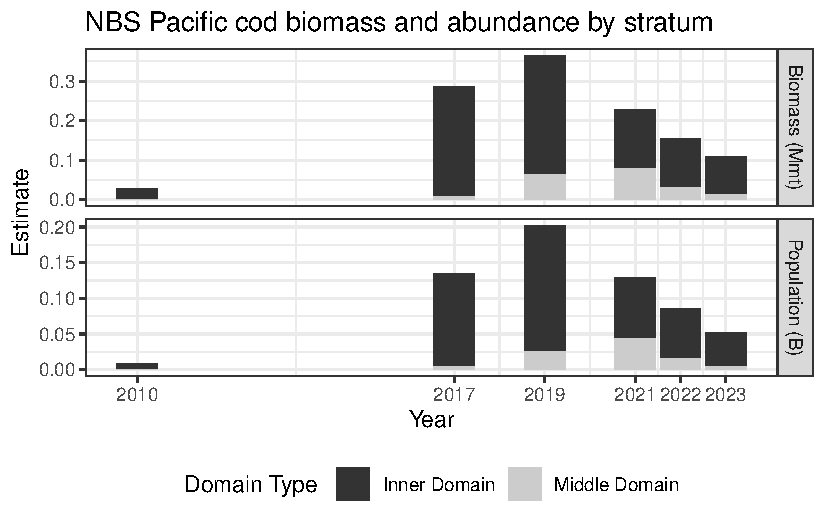
\includegraphics{content/akfin-oracle-sql-r_files/figure-pdf/test-4-fig-1.pdf}

}

\caption{Ex. 4: NBS Pacific cod biomass and abundance.}

\end{figure}

\hypertarget{ex.-5-goa-pacific-ocean-perch-biomass-and-line-plot}{%
\subsection{Ex. 5: GOA Pacific Ocean perch biomass and line
plot}\label{ex.-5-goa-pacific-ocean-perch-biomass-and-line-plot}}

Pacific Ocean perch biomass totals for GOA between 1984-2021 from
\texttt{GAP\_PRODUCTS.AKFIN\_BIOMASS}

\begin{Shaded}
\begin{Highlighting}[]
\NormalTok{dat }\OtherTok{\textless{}{-}}\NormalTok{ RODBC}\SpecialCharTok{::}\FunctionTok{sqlQuery}\NormalTok{(}\AttributeTok{channel =}\NormalTok{ channel, }
                       \AttributeTok{query =} 
\StringTok{"SELECT }
\StringTok{SURVEY\_DEFINITION\_ID, }
\StringTok{BIOMASS\_MT, }
\StringTok{BIOMASS\_VAR, }
\StringTok{YEAR}
\StringTok{FROM GAP\_PRODUCTS.AKFIN\_BIOMASS}
\StringTok{WHERE SPECIES\_CODE = 30060 }
\StringTok{AND SURVEY\_DEFINITION\_ID = 47 }
\StringTok{AND AREA\_ID = 99903 }
\StringTok{AND YEAR BETWEEN 1984 AND 2023;"}\NormalTok{) }\SpecialCharTok{\%\textgreater{}\%} 
\NormalTok{  janitor}\SpecialCharTok{::}\FunctionTok{clean\_names}\NormalTok{() }\SpecialCharTok{\%\textgreater{}\%} 
\NormalTok{  dplyr}\SpecialCharTok{::}\FunctionTok{mutate}\NormalTok{(}\AttributeTok{biomass\_kmt =}\NormalTok{ biomass\_mt}\SpecialCharTok{/}\DecValTok{1000}\NormalTok{, }
                \CommentTok{\# **approximate** 95\% confidence interval}
                \AttributeTok{biomass\_kci\_up =}\NormalTok{ (biomass\_mt }\SpecialCharTok{+}\NormalTok{ (}\DecValTok{2}\SpecialCharTok{*}\FunctionTok{sqrt}\NormalTok{(biomass\_var)))}\SpecialCharTok{/}\DecValTok{1000}\NormalTok{, }
                \AttributeTok{biomass\_kci\_dw =}\NormalTok{ (biomass\_mt }\SpecialCharTok{{-}}\NormalTok{ (}\DecValTok{2}\SpecialCharTok{*}\FunctionTok{sqrt}\NormalTok{(biomass\_var)))}\SpecialCharTok{/}\DecValTok{1000}\NormalTok{) }
\end{Highlighting}
\end{Shaded}

\begin{Shaded}
\begin{Highlighting}[]
\NormalTok{flextable}\SpecialCharTok{::}\FunctionTok{flextable}\NormalTok{(}\FunctionTok{head}\NormalTok{(dat)) }\SpecialCharTok{\%\textgreater{}\%}
  \FunctionTok{theme\_zebra}\NormalTok{() }\SpecialCharTok{\%\textgreater{}\%}
\NormalTok{  flextable}\SpecialCharTok{::}\FunctionTok{colformat\_num}\NormalTok{(}\AttributeTok{x =}\NormalTok{ ., }\AttributeTok{j =} \StringTok{"year"}\NormalTok{, }\AttributeTok{big.mark =} \StringTok{""}\NormalTok{)}
\end{Highlighting}
\end{Shaded}

\global\setlength{\Oldarrayrulewidth}{\arrayrulewidth}

\global\setlength{\Oldtabcolsep}{\tabcolsep}

\setlength{\tabcolsep}{0pt}

\renewcommand*{\arraystretch}{1.5}



\providecommand{\ascline}[3]{\noalign{\global\arrayrulewidth #1}\arrayrulecolor[HTML]{#2}\cline{#3}}

\begin{longtable}[c]{|p{0.75in}|p{0.75in}|p{0.75in}|p{0.75in}|p{0.75in}|p{0.75in}|p{0.75in}}
\caption{Ex. 5: GOA Pacific Ocean perch biomass and line plot.}\tabularnewline




\hhline{>{\arrayrulecolor[HTML]{000000}\global\arrayrulewidth=0pt}->{\arrayrulecolor[HTML]{000000}\global\arrayrulewidth=0pt}->{\arrayrulecolor[HTML]{000000}\global\arrayrulewidth=0pt}->{\arrayrulecolor[HTML]{000000}\global\arrayrulewidth=0pt}->{\arrayrulecolor[HTML]{000000}\global\arrayrulewidth=0pt}->{\arrayrulecolor[HTML]{000000}\global\arrayrulewidth=0pt}->{\arrayrulecolor[HTML]{000000}\global\arrayrulewidth=0pt}-}

\multicolumn{1}{>{\cellcolor[HTML]{CFCFCF}\raggedleft}m{\dimexpr 0.75in+0\tabcolsep}}{\textcolor[HTML]{000000}{\fontsize{11}{11}\selectfont{\textbf{survey\_definition\_id}}}} & \multicolumn{1}{>{\cellcolor[HTML]{CFCFCF}\raggedleft}m{\dimexpr 0.75in+0\tabcolsep}}{\textcolor[HTML]{000000}{\fontsize{11}{11}\selectfont{\textbf{biomass\_mt}}}} & \multicolumn{1}{>{\cellcolor[HTML]{CFCFCF}\raggedleft}m{\dimexpr 0.75in+0\tabcolsep}}{\textcolor[HTML]{000000}{\fontsize{11}{11}\selectfont{\textbf{biomass\_var}}}} & \multicolumn{1}{>{\cellcolor[HTML]{CFCFCF}\raggedleft}m{\dimexpr 0.75in+0\tabcolsep}}{\textcolor[HTML]{000000}{\fontsize{11}{11}\selectfont{\textbf{year}}}} & \multicolumn{1}{>{\cellcolor[HTML]{CFCFCF}\raggedleft}m{\dimexpr 0.75in+0\tabcolsep}}{\textcolor[HTML]{000000}{\fontsize{11}{11}\selectfont{\textbf{biomass\_kmt}}}} & \multicolumn{1}{>{\cellcolor[HTML]{CFCFCF}\raggedleft}m{\dimexpr 0.75in+0\tabcolsep}}{\textcolor[HTML]{000000}{\fontsize{11}{11}\selectfont{\textbf{biomass\_kci\_up}}}} & \multicolumn{1}{>{\cellcolor[HTML]{CFCFCF}\raggedleft}m{\dimexpr 0.75in+0\tabcolsep}}{\textcolor[HTML]{000000}{\fontsize{11}{11}\selectfont{\textbf{biomass\_kci\_dw}}}} \\

\noalign{\global\arrayrulewidth 0pt}\arrayrulecolor[HTML]{000000}

\endfirsthead 

\hhline{>{\arrayrulecolor[HTML]{000000}\global\arrayrulewidth=0pt}->{\arrayrulecolor[HTML]{000000}\global\arrayrulewidth=0pt}->{\arrayrulecolor[HTML]{000000}\global\arrayrulewidth=0pt}->{\arrayrulecolor[HTML]{000000}\global\arrayrulewidth=0pt}->{\arrayrulecolor[HTML]{000000}\global\arrayrulewidth=0pt}->{\arrayrulecolor[HTML]{000000}\global\arrayrulewidth=0pt}->{\arrayrulecolor[HTML]{000000}\global\arrayrulewidth=0pt}-}

\multicolumn{1}{>{\cellcolor[HTML]{CFCFCF}\raggedleft}m{\dimexpr 0.75in+0\tabcolsep}}{\textcolor[HTML]{000000}{\fontsize{11}{11}\selectfont{\textbf{survey\_definition\_id}}}} & \multicolumn{1}{>{\cellcolor[HTML]{CFCFCF}\raggedleft}m{\dimexpr 0.75in+0\tabcolsep}}{\textcolor[HTML]{000000}{\fontsize{11}{11}\selectfont{\textbf{biomass\_mt}}}} & \multicolumn{1}{>{\cellcolor[HTML]{CFCFCF}\raggedleft}m{\dimexpr 0.75in+0\tabcolsep}}{\textcolor[HTML]{000000}{\fontsize{11}{11}\selectfont{\textbf{biomass\_var}}}} & \multicolumn{1}{>{\cellcolor[HTML]{CFCFCF}\raggedleft}m{\dimexpr 0.75in+0\tabcolsep}}{\textcolor[HTML]{000000}{\fontsize{11}{11}\selectfont{\textbf{year}}}} & \multicolumn{1}{>{\cellcolor[HTML]{CFCFCF}\raggedleft}m{\dimexpr 0.75in+0\tabcolsep}}{\textcolor[HTML]{000000}{\fontsize{11}{11}\selectfont{\textbf{biomass\_kmt}}}} & \multicolumn{1}{>{\cellcolor[HTML]{CFCFCF}\raggedleft}m{\dimexpr 0.75in+0\tabcolsep}}{\textcolor[HTML]{000000}{\fontsize{11}{11}\selectfont{\textbf{biomass\_kci\_up}}}} & \multicolumn{1}{>{\cellcolor[HTML]{CFCFCF}\raggedleft}m{\dimexpr 0.75in+0\tabcolsep}}{\textcolor[HTML]{000000}{\fontsize{11}{11}\selectfont{\textbf{biomass\_kci\_dw}}}} \\

\noalign{\global\arrayrulewidth 0pt}\arrayrulecolor[HTML]{000000}

\endhead



\multicolumn{1}{>{\cellcolor[HTML]{EFEFEF}\raggedleft}m{\dimexpr 0.75in+0\tabcolsep}}{\textcolor[HTML]{000000}{\fontsize{11}{11}\selectfont{47}}} & \multicolumn{1}{>{\cellcolor[HTML]{EFEFEF}\raggedleft}m{\dimexpr 0.75in+0\tabcolsep}}{\textcolor[HTML]{000000}{\fontsize{11}{11}\selectfont{483,622.6}}} & \multicolumn{1}{>{\cellcolor[HTML]{EFEFEF}\raggedleft}m{\dimexpr 0.75in+0\tabcolsep}}{\textcolor[HTML]{000000}{\fontsize{11}{11}\selectfont{11,803,384,787}}} & \multicolumn{1}{>{\cellcolor[HTML]{EFEFEF}\raggedleft}m{\dimexpr 0.75in+0\tabcolsep}}{\textcolor[HTML]{000000}{\fontsize{11}{11}\selectfont{1993}}} & \multicolumn{1}{>{\cellcolor[HTML]{EFEFEF}\raggedleft}m{\dimexpr 0.75in+0\tabcolsep}}{\textcolor[HTML]{000000}{\fontsize{11}{11}\selectfont{483.6226}}} & \multicolumn{1}{>{\cellcolor[HTML]{EFEFEF}\raggedleft}m{\dimexpr 0.75in+0\tabcolsep}}{\textcolor[HTML]{000000}{\fontsize{11}{11}\selectfont{700.9093}}} & \multicolumn{1}{>{\cellcolor[HTML]{EFEFEF}\raggedleft}m{\dimexpr 0.75in+0\tabcolsep}}{\textcolor[HTML]{000000}{\fontsize{11}{11}\selectfont{266.33581}}} \\

\noalign{\global\arrayrulewidth 0pt}\arrayrulecolor[HTML]{000000}





\multicolumn{1}{>{\raggedleft}m{\dimexpr 0.75in+0\tabcolsep}}{\textcolor[HTML]{000000}{\fontsize{11}{11}\selectfont{47}}} & \multicolumn{1}{>{\raggedleft}m{\dimexpr 0.75in+0\tabcolsep}}{\textcolor[HTML]{000000}{\fontsize{11}{11}\selectfont{771,412.8}}} & \multicolumn{1}{>{\raggedleft}m{\dimexpr 0.75in+0\tabcolsep}}{\textcolor[HTML]{000000}{\fontsize{11}{11}\selectfont{41,434,152,202}}} & \multicolumn{1}{>{\raggedleft}m{\dimexpr 0.75in+0\tabcolsep}}{\textcolor[HTML]{000000}{\fontsize{11}{11}\selectfont{1996}}} & \multicolumn{1}{>{\raggedleft}m{\dimexpr 0.75in+0\tabcolsep}}{\textcolor[HTML]{000000}{\fontsize{11}{11}\selectfont{771.4128}}} & \multicolumn{1}{>{\raggedleft}m{\dimexpr 0.75in+0\tabcolsep}}{\textcolor[HTML]{000000}{\fontsize{11}{11}\selectfont{1,178.5204}}} & \multicolumn{1}{>{\raggedleft}m{\dimexpr 0.75in+0\tabcolsep}}{\textcolor[HTML]{000000}{\fontsize{11}{11}\selectfont{364.30515}}} \\

\noalign{\global\arrayrulewidth 0pt}\arrayrulecolor[HTML]{000000}





\multicolumn{1}{>{\cellcolor[HTML]{EFEFEF}\raggedleft}m{\dimexpr 0.75in+0\tabcolsep}}{\textcolor[HTML]{000000}{\fontsize{11}{11}\selectfont{47}}} & \multicolumn{1}{>{\cellcolor[HTML]{EFEFEF}\raggedleft}m{\dimexpr 0.75in+0\tabcolsep}}{\textcolor[HTML]{000000}{\fontsize{11}{11}\selectfont{727,063.5}}} & \multicolumn{1}{>{\cellcolor[HTML]{EFEFEF}\raggedleft}m{\dimexpr 0.75in+0\tabcolsep}}{\textcolor[HTML]{000000}{\fontsize{11}{11}\selectfont{150,983,542,178}}} & \multicolumn{1}{>{\cellcolor[HTML]{EFEFEF}\raggedleft}m{\dimexpr 0.75in+0\tabcolsep}}{\textcolor[HTML]{000000}{\fontsize{11}{11}\selectfont{1999}}} & \multicolumn{1}{>{\cellcolor[HTML]{EFEFEF}\raggedleft}m{\dimexpr 0.75in+0\tabcolsep}}{\textcolor[HTML]{000000}{\fontsize{11}{11}\selectfont{727.0635}}} & \multicolumn{1}{>{\cellcolor[HTML]{EFEFEF}\raggedleft}m{\dimexpr 0.75in+0\tabcolsep}}{\textcolor[HTML]{000000}{\fontsize{11}{11}\selectfont{1,504.1955}}} & \multicolumn{1}{>{\cellcolor[HTML]{EFEFEF}\raggedleft}m{\dimexpr 0.75in+0\tabcolsep}}{\textcolor[HTML]{000000}{\fontsize{11}{11}\selectfont{-50.06854}}} \\

\noalign{\global\arrayrulewidth 0pt}\arrayrulecolor[HTML]{000000}





\multicolumn{1}{>{\raggedleft}m{\dimexpr 0.75in+0\tabcolsep}}{\textcolor[HTML]{000000}{\fontsize{11}{11}\selectfont{47}}} & \multicolumn{1}{>{\raggedleft}m{\dimexpr 0.75in+0\tabcolsep}}{\textcolor[HTML]{000000}{\fontsize{11}{11}\selectfont{673,155.1}}} & \multicolumn{1}{>{\raggedleft}m{\dimexpr 0.75in+0\tabcolsep}}{\textcolor[HTML]{000000}{\fontsize{11}{11}\selectfont{49,285,342,922}}} & \multicolumn{1}{>{\raggedleft}m{\dimexpr 0.75in+0\tabcolsep}}{\textcolor[HTML]{000000}{\fontsize{11}{11}\selectfont{2001}}} & \multicolumn{1}{>{\raggedleft}m{\dimexpr 0.75in+0\tabcolsep}}{\textcolor[HTML]{000000}{\fontsize{11}{11}\selectfont{673.1551}}} & \multicolumn{1}{>{\raggedleft}m{\dimexpr 0.75in+0\tabcolsep}}{\textcolor[HTML]{000000}{\fontsize{11}{11}\selectfont{1,117.1611}}} & \multicolumn{1}{>{\raggedleft}m{\dimexpr 0.75in+0\tabcolsep}}{\textcolor[HTML]{000000}{\fontsize{11}{11}\selectfont{229.14901}}} \\

\noalign{\global\arrayrulewidth 0pt}\arrayrulecolor[HTML]{000000}





\multicolumn{1}{>{\cellcolor[HTML]{EFEFEF}\raggedleft}m{\dimexpr 0.75in+0\tabcolsep}}{\textcolor[HTML]{000000}{\fontsize{11}{11}\selectfont{47}}} & \multicolumn{1}{>{\cellcolor[HTML]{EFEFEF}\raggedleft}m{\dimexpr 0.75in+0\tabcolsep}}{\textcolor[HTML]{000000}{\fontsize{11}{11}\selectfont{457,421.6}}} & \multicolumn{1}{>{\cellcolor[HTML]{EFEFEF}\raggedleft}m{\dimexpr 0.75in+0\tabcolsep}}{\textcolor[HTML]{000000}{\fontsize{11}{11}\selectfont{5,186,126,529}}} & \multicolumn{1}{>{\cellcolor[HTML]{EFEFEF}\raggedleft}m{\dimexpr 0.75in+0\tabcolsep}}{\textcolor[HTML]{000000}{\fontsize{11}{11}\selectfont{2003}}} & \multicolumn{1}{>{\cellcolor[HTML]{EFEFEF}\raggedleft}m{\dimexpr 0.75in+0\tabcolsep}}{\textcolor[HTML]{000000}{\fontsize{11}{11}\selectfont{457.4216}}} & \multicolumn{1}{>{\cellcolor[HTML]{EFEFEF}\raggedleft}m{\dimexpr 0.75in+0\tabcolsep}}{\textcolor[HTML]{000000}{\fontsize{11}{11}\selectfont{601.4511}}} & \multicolumn{1}{>{\cellcolor[HTML]{EFEFEF}\raggedleft}m{\dimexpr 0.75in+0\tabcolsep}}{\textcolor[HTML]{000000}{\fontsize{11}{11}\selectfont{313.39204}}} \\

\noalign{\global\arrayrulewidth 0pt}\arrayrulecolor[HTML]{000000}





\multicolumn{1}{>{\raggedleft}m{\dimexpr 0.75in+0\tabcolsep}}{\textcolor[HTML]{000000}{\fontsize{11}{11}\selectfont{47}}} & \multicolumn{1}{>{\raggedleft}m{\dimexpr 0.75in+0\tabcolsep}}{\textcolor[HTML]{000000}{\fontsize{11}{11}\selectfont{764,901.4}}} & \multicolumn{1}{>{\raggedleft}m{\dimexpr 0.75in+0\tabcolsep}}{\textcolor[HTML]{000000}{\fontsize{11}{11}\selectfont{21,499,807,010}}} & \multicolumn{1}{>{\raggedleft}m{\dimexpr 0.75in+0\tabcolsep}}{\textcolor[HTML]{000000}{\fontsize{11}{11}\selectfont{2005}}} & \multicolumn{1}{>{\raggedleft}m{\dimexpr 0.75in+0\tabcolsep}}{\textcolor[HTML]{000000}{\fontsize{11}{11}\selectfont{764.9014}}} & \multicolumn{1}{>{\raggedleft}m{\dimexpr 0.75in+0\tabcolsep}}{\textcolor[HTML]{000000}{\fontsize{11}{11}\selectfont{1,058.1577}}} & \multicolumn{1}{>{\raggedleft}m{\dimexpr 0.75in+0\tabcolsep}}{\textcolor[HTML]{000000}{\fontsize{11}{11}\selectfont{471.64517}}} \\

\noalign{\global\arrayrulewidth 0pt}\arrayrulecolor[HTML]{000000}





\end{longtable}



\arrayrulecolor[HTML]{000000}

\global\setlength{\arrayrulewidth}{\Oldarrayrulewidth}

\global\setlength{\tabcolsep}{\Oldtabcolsep}

\renewcommand*{\arraystretch}{1}

\begin{Shaded}
\begin{Highlighting}[]
\NormalTok{a\_mean }\OtherTok{\textless{}{-}}\NormalTok{ dat }\SpecialCharTok{\%\textgreater{}\%} 
\NormalTok{  dplyr}\SpecialCharTok{::}\FunctionTok{group\_by}\NormalTok{(survey\_definition\_id) }\SpecialCharTok{\%\textgreater{}\%} 
\NormalTok{  dplyr}\SpecialCharTok{::}\FunctionTok{summarise}\NormalTok{(}\AttributeTok{biomass\_kmt =} \FunctionTok{mean}\NormalTok{(biomass\_kmt, }\AttributeTok{na.rm =} \ConstantTok{TRUE}\NormalTok{), }
                   \AttributeTok{minyr =} \FunctionTok{min}\NormalTok{(year, }\AttributeTok{na.rm =} \ConstantTok{TRUE}\NormalTok{), }
                   \AttributeTok{maxyr =} \FunctionTok{max}\NormalTok{(year, }\AttributeTok{na.rm =} \ConstantTok{TRUE}\NormalTok{)) }

\NormalTok{figure }\OtherTok{\textless{}{-}}
  \FunctionTok{ggplot}\NormalTok{(}\AttributeTok{data =}\NormalTok{ dat, }
         \AttributeTok{mapping =} \FunctionTok{aes}\NormalTok{(}\AttributeTok{x =}\NormalTok{ year, }
                       \AttributeTok{y =}\NormalTok{ biomass\_kmt)) }\SpecialCharTok{+}
\NormalTok{  ggplot2}\SpecialCharTok{::}\FunctionTok{geom\_point}\NormalTok{(}\AttributeTok{size =} \FloatTok{2.5}\NormalTok{, }\AttributeTok{color =} \StringTok{"grey40"}\NormalTok{) }\SpecialCharTok{+} 
\NormalTok{  ggplot2}\SpecialCharTok{::}\FunctionTok{scale\_x\_continuous}\NormalTok{(}
    \AttributeTok{name =} \StringTok{"Year"}\NormalTok{, }
    \AttributeTok{labels =}\NormalTok{ scales}\SpecialCharTok{::}\FunctionTok{label\_number}\NormalTok{(}
      \AttributeTok{accuracy =} \DecValTok{1}\NormalTok{, }
      \AttributeTok{big.mark =} \StringTok{""}\NormalTok{))   }\SpecialCharTok{+}
\NormalTok{  ggplot2}\SpecialCharTok{::}\FunctionTok{scale\_y\_continuous}\NormalTok{(}
    \AttributeTok{name =} \StringTok{"Biomass (Kmt)"}\NormalTok{, }
    \AttributeTok{labels =}\NormalTok{ comma) }\SpecialCharTok{+}
\NormalTok{  ggplot2}\SpecialCharTok{::}\FunctionTok{geom\_segment}\NormalTok{(}
    \AttributeTok{data =}\NormalTok{ a\_mean,}
    \AttributeTok{mapping =} \FunctionTok{aes}\NormalTok{(}\AttributeTok{x =}\NormalTok{ minyr, }
                  \AttributeTok{xend =}\NormalTok{ maxyr, }
                  \AttributeTok{y =}\NormalTok{ biomass\_kmt, }
                  \AttributeTok{yend =}\NormalTok{ biomass\_kmt),}
    \AttributeTok{linetype =} \StringTok{"dashed"}\NormalTok{, }
    \AttributeTok{linewidth =} \DecValTok{2}\NormalTok{) }\SpecialCharTok{+}
\NormalTok{  ggplot2}\SpecialCharTok{::}\FunctionTok{geom\_errorbar}\NormalTok{(}
    \AttributeTok{mapping =} \FunctionTok{aes}\NormalTok{(}\AttributeTok{ymin =}\NormalTok{ biomass\_kci\_dw, }\AttributeTok{ymax =}\NormalTok{ biomass\_kci\_up),}
                 \AttributeTok{position =} \FunctionTok{position\_dodge}\NormalTok{(.}\DecValTok{9}\NormalTok{),}
    \AttributeTok{alpha =} \FloatTok{0.5}\NormalTok{, }\AttributeTok{width=}\NormalTok{.}\DecValTok{2}\NormalTok{) }\SpecialCharTok{+}
\NormalTok{  ggplot2}\SpecialCharTok{::}\FunctionTok{ggtitle}\NormalTok{(}
    \AttributeTok{label =} \StringTok{"GOA Pacific Ocean Perch Biomass 1984{-}2021"}\NormalTok{, }
    \AttributeTok{subtitle =} \FunctionTok{paste0}\NormalTok{(}\StringTok{"Mean = "}\NormalTok{, }
                      \FunctionTok{formatC}\NormalTok{(}\AttributeTok{x =}\NormalTok{ a\_mean}\SpecialCharTok{$}\NormalTok{biomass\_kmt, }
                              \AttributeTok{digits =} \DecValTok{2}\NormalTok{, }
                              \AttributeTok{big.mark =} \StringTok{","}\NormalTok{, }
                              \AttributeTok{format =} \StringTok{"f"}\NormalTok{), }
                      \StringTok{" Kmt"}\NormalTok{)) }\SpecialCharTok{+}
\NormalTok{  ggplot2}\SpecialCharTok{::}\FunctionTok{theme\_bw}\NormalTok{()}

\NormalTok{figure}
\end{Highlighting}
\end{Shaded}

\begin{figure}[H]

{\centering 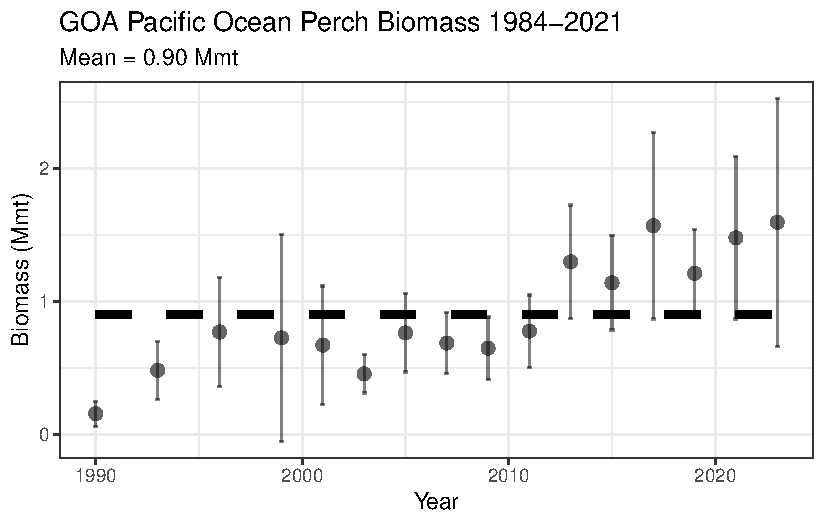
\includegraphics{content/akfin-oracle-sql-r_files/figure-pdf/test-5-fig-1.pdf}

}

\caption{Ex. 5: GOA Pacific Ocean perch biomass and line plot.}

\end{figure}

\hypertarget{ex.-6-ebs-pacific-ocean-perch-cpue-and-akgfmaps-map}{%
\subsection{\texorpdfstring{Ex. 6: EBS Pacific Ocean perch CPUE and
\href{https://github.com/afsc-gap-products/akgfmaps}{\texttt{akgfmaps}}
map}{Ex. 6: EBS Pacific Ocean perch CPUE and akgfmaps map}}\label{ex.-6-ebs-pacific-ocean-perch-cpue-and-akgfmaps-map}}

Pacific Ocean perch catch-per-unit-effort estimates for EBS in 2021 from
\texttt{GAP\_PRODUCTS.AKFIN\_CPUE} and map constructed using
\href{https://github.com/afsc-gap-products/akgfmaps}{\texttt{akgfmaps}}.
Here, we'll use AKFIN HAUL and CRUISES data also included in this repo,
for convenience, though they are very similar to their \texttt{RACEBASE}
analogs.

\begin{Shaded}
\begin{Highlighting}[]
\NormalTok{dat }\OtherTok{\textless{}{-}}\NormalTok{ RODBC}\SpecialCharTok{::}\FunctionTok{sqlQuery}\NormalTok{(}\AttributeTok{channel =}\NormalTok{ channel, }
                       \AttributeTok{query =} 
\StringTok{"SELECT }
\StringTok{(cp.CPUE\_KGKM2/100) CPUE\_KGHA, {-}{-} akgfmaps is expecting hectares}
\StringTok{hh.LATITUDE\_DD\_START LATITUDE,}
\StringTok{hh.LONGITUDE\_DD\_START LONGITUDE}

\StringTok{FROM GAP\_PRODUCTS.AKFIN\_CPUE cp}

\StringTok{{-}{-} Use HAUL data to obtain LATITUDE \& LONGITUDE and connect to cruisejoin}
\StringTok{LEFT JOIN GAP\_PRODUCTS.AKFIN\_HAUL hh}
\StringTok{ON cp.HAULJOIN = hh.HAULJOIN}

\StringTok{{-}{-} Use CRUISES data to obtain YEAR and SURVEY\_DEFINITION\_ID}
\StringTok{LEFT JOIN GAP\_PRODUCTS.AKFIN\_CRUISE cc}
\StringTok{ON hh.CRUISEJOIN = cc.CRUISEJOIN}

\StringTok{WHERE cp.SPECIES\_CODE = 30060 }
\StringTok{AND cc.SURVEY\_DEFINITION\_ID = 98 }
\StringTok{AND cc.YEAR = 2021;"}\NormalTok{)}
\end{Highlighting}
\end{Shaded}

\begin{Shaded}
\begin{Highlighting}[]
\NormalTok{flextable}\SpecialCharTok{::}\FunctionTok{flextable}\NormalTok{(}\FunctionTok{head}\NormalTok{(dat)) }\SpecialCharTok{\%\textgreater{}\%} \FunctionTok{theme\_zebra}\NormalTok{()}
\end{Highlighting}
\end{Shaded}

\global\setlength{\Oldarrayrulewidth}{\arrayrulewidth}

\global\setlength{\Oldtabcolsep}{\tabcolsep}

\setlength{\tabcolsep}{0pt}

\renewcommand*{\arraystretch}{1.5}



\providecommand{\ascline}[3]{\noalign{\global\arrayrulewidth #1}\arrayrulecolor[HTML]{#2}\cline{#3}}

\begin{longtable}[c]{|p{0.75in}|p{0.75in}|p{0.75in}}
\caption{Ex. 6: EBS Pacific Ocean perch CPUE and
\href{https://github.com/afsc-gap-products/akgfmaps}{\texttt{akgfmaps}}
map.}\tabularnewline




\hhline{>{\arrayrulecolor[HTML]{000000}\global\arrayrulewidth=0pt}->{\arrayrulecolor[HTML]{000000}\global\arrayrulewidth=0pt}->{\arrayrulecolor[HTML]{000000}\global\arrayrulewidth=0pt}-}

\multicolumn{1}{>{\cellcolor[HTML]{CFCFCF}\raggedleft}m{\dimexpr 0.75in+0\tabcolsep}}{\textcolor[HTML]{000000}{\fontsize{11}{11}\selectfont{\textbf{CPUE\_KGHA}}}} & \multicolumn{1}{>{\cellcolor[HTML]{CFCFCF}\raggedleft}m{\dimexpr 0.75in+0\tabcolsep}}{\textcolor[HTML]{000000}{\fontsize{11}{11}\selectfont{\textbf{LATITUDE}}}} & \multicolumn{1}{>{\cellcolor[HTML]{CFCFCF}\raggedleft}m{\dimexpr 0.75in+0\tabcolsep}}{\textcolor[HTML]{000000}{\fontsize{11}{11}\selectfont{\textbf{LONGITUDE}}}} \\

\noalign{\global\arrayrulewidth 0pt}\arrayrulecolor[HTML]{000000}

\endfirsthead 

\hhline{>{\arrayrulecolor[HTML]{000000}\global\arrayrulewidth=0pt}->{\arrayrulecolor[HTML]{000000}\global\arrayrulewidth=0pt}->{\arrayrulecolor[HTML]{000000}\global\arrayrulewidth=0pt}-}

\multicolumn{1}{>{\cellcolor[HTML]{CFCFCF}\raggedleft}m{\dimexpr 0.75in+0\tabcolsep}}{\textcolor[HTML]{000000}{\fontsize{11}{11}\selectfont{\textbf{CPUE\_KGHA}}}} & \multicolumn{1}{>{\cellcolor[HTML]{CFCFCF}\raggedleft}m{\dimexpr 0.75in+0\tabcolsep}}{\textcolor[HTML]{000000}{\fontsize{11}{11}\selectfont{\textbf{LATITUDE}}}} & \multicolumn{1}{>{\cellcolor[HTML]{CFCFCF}\raggedleft}m{\dimexpr 0.75in+0\tabcolsep}}{\textcolor[HTML]{000000}{\fontsize{11}{11}\selectfont{\textbf{LONGITUDE}}}} \\

\noalign{\global\arrayrulewidth 0pt}\arrayrulecolor[HTML]{000000}

\endhead



\multicolumn{1}{>{\cellcolor[HTML]{EFEFEF}\raggedleft}m{\dimexpr 0.75in+0\tabcolsep}}{\textcolor[HTML]{000000}{\fontsize{11}{11}\selectfont{0.0000000}}} & \multicolumn{1}{>{\cellcolor[HTML]{EFEFEF}\raggedleft}m{\dimexpr 0.75in+0\tabcolsep}}{\textcolor[HTML]{000000}{\fontsize{11}{11}\selectfont{58.75863}}} & \multicolumn{1}{>{\cellcolor[HTML]{EFEFEF}\raggedleft}m{\dimexpr 0.75in+0\tabcolsep}}{\textcolor[HTML]{000000}{\fontsize{11}{11}\selectfont{-174.9285}}} \\

\noalign{\global\arrayrulewidth 0pt}\arrayrulecolor[HTML]{000000}





\multicolumn{1}{>{\raggedleft}m{\dimexpr 0.75in+0\tabcolsep}}{\textcolor[HTML]{000000}{\fontsize{11}{11}\selectfont{0.2813533}}} & \multicolumn{1}{>{\raggedleft}m{\dimexpr 0.75in+0\tabcolsep}}{\textcolor[HTML]{000000}{\fontsize{11}{11}\selectfont{57.32545}}} & \multicolumn{1}{>{\raggedleft}m{\dimexpr 0.75in+0\tabcolsep}}{\textcolor[HTML]{000000}{\fontsize{11}{11}\selectfont{-173.3217}}} \\

\noalign{\global\arrayrulewidth 0pt}\arrayrulecolor[HTML]{000000}





\multicolumn{1}{>{\cellcolor[HTML]{EFEFEF}\raggedleft}m{\dimexpr 0.75in+0\tabcolsep}}{\textcolor[HTML]{000000}{\fontsize{11}{11}\selectfont{0.0000000}}} & \multicolumn{1}{>{\cellcolor[HTML]{EFEFEF}\raggedleft}m{\dimexpr 0.75in+0\tabcolsep}}{\textcolor[HTML]{000000}{\fontsize{11}{11}\selectfont{57.64161}}} & \multicolumn{1}{>{\cellcolor[HTML]{EFEFEF}\raggedleft}m{\dimexpr 0.75in+0\tabcolsep}}{\textcolor[HTML]{000000}{\fontsize{11}{11}\selectfont{-172.7963}}} \\

\noalign{\global\arrayrulewidth 0pt}\arrayrulecolor[HTML]{000000}





\multicolumn{1}{>{\raggedleft}m{\dimexpr 0.75in+0\tabcolsep}}{\textcolor[HTML]{000000}{\fontsize{11}{11}\selectfont{0.0000000}}} & \multicolumn{1}{>{\raggedleft}m{\dimexpr 0.75in+0\tabcolsep}}{\textcolor[HTML]{000000}{\fontsize{11}{11}\selectfont{59.67831}}} & \multicolumn{1}{>{\raggedleft}m{\dimexpr 0.75in+0\tabcolsep}}{\textcolor[HTML]{000000}{\fontsize{11}{11}\selectfont{-172.5754}}} \\

\noalign{\global\arrayrulewidth 0pt}\arrayrulecolor[HTML]{000000}





\multicolumn{1}{>{\cellcolor[HTML]{EFEFEF}\raggedleft}m{\dimexpr 0.75in+0\tabcolsep}}{\textcolor[HTML]{000000}{\fontsize{11}{11}\selectfont{0.0000000}}} & \multicolumn{1}{>{\cellcolor[HTML]{EFEFEF}\raggedleft}m{\dimexpr 0.75in+0\tabcolsep}}{\textcolor[HTML]{000000}{\fontsize{11}{11}\selectfont{60.96936}}} & \multicolumn{1}{>{\cellcolor[HTML]{EFEFEF}\raggedleft}m{\dimexpr 0.75in+0\tabcolsep}}{\textcolor[HTML]{000000}{\fontsize{11}{11}\selectfont{-174.8760}}} \\

\noalign{\global\arrayrulewidth 0pt}\arrayrulecolor[HTML]{000000}





\multicolumn{1}{>{\raggedleft}m{\dimexpr 0.75in+0\tabcolsep}}{\textcolor[HTML]{000000}{\fontsize{11}{11}\selectfont{0.0000000}}} & \multicolumn{1}{>{\raggedleft}m{\dimexpr 0.75in+0\tabcolsep}}{\textcolor[HTML]{000000}{\fontsize{11}{11}\selectfont{58.64012}}} & \multicolumn{1}{>{\raggedleft}m{\dimexpr 0.75in+0\tabcolsep}}{\textcolor[HTML]{000000}{\fontsize{11}{11}\selectfont{-173.5922}}} \\

\noalign{\global\arrayrulewidth 0pt}\arrayrulecolor[HTML]{000000}





\end{longtable}



\arrayrulecolor[HTML]{000000}

\global\setlength{\arrayrulewidth}{\Oldarrayrulewidth}

\global\setlength{\tabcolsep}{\Oldtabcolsep}

\renewcommand*{\arraystretch}{1}

\begin{Shaded}
\begin{Highlighting}[]
\CommentTok{\# devtools::install\_github("afsc{-}gap{-}products/akgfmaps", build\_vignettes = TRUE)}
\FunctionTok{library}\NormalTok{(akgfmaps)}

\NormalTok{figure }\OtherTok{\textless{}{-}}\NormalTok{ akgfmaps}\SpecialCharTok{::}\FunctionTok{make\_idw\_map}\NormalTok{(}
  \AttributeTok{x =}\NormalTok{ dat, }\CommentTok{\# Pass data as a data frame}
  \AttributeTok{region =} \StringTok{"bs.south"}\NormalTok{, }\CommentTok{\# Predefined EBS area}
  \AttributeTok{set.breaks =} \StringTok{"jenks"}\NormalTok{, }\CommentTok{\# Gets Jenks breaks from classint::classIntervals()}
  \AttributeTok{in.crs =} \StringTok{"+proj=longlat"}\NormalTok{, }\CommentTok{\# Set input coordinate reference system}
  \AttributeTok{out.crs =} \StringTok{"EPSG:3338"}\NormalTok{, }\CommentTok{\# Set output coordinate reference system}
  \AttributeTok{grid.cell =} \FunctionTok{c}\NormalTok{(}\DecValTok{20000}\NormalTok{, }\DecValTok{20000}\NormalTok{), }\CommentTok{\# 20x20km grid}
  \AttributeTok{key.title =} \StringTok{"Pacific Ocean perch"}\NormalTok{) }\CommentTok{\# Include in the legend title}
\end{Highlighting}
\end{Shaded}

\begin{verbatim}
[inverse distance weighted interpolation]
[inverse distance weighted interpolation]
\end{verbatim}

\begin{Shaded}
\begin{Highlighting}[]
\NormalTok{figure}\SpecialCharTok{$}\NormalTok{plot }\SpecialCharTok{+} 
\NormalTok{  ggplot2}\SpecialCharTok{::}\FunctionTok{guides}\NormalTok{(}\AttributeTok{fill=}\FunctionTok{guide\_legend}\NormalTok{(}\AttributeTok{title =} \StringTok{"Pacific Ocean perch}\SpecialCharTok{\textbackslash{}n}\StringTok{CPUE (kg/km2)"}\NormalTok{))  }\SpecialCharTok{|\textgreater{}}   
  \FunctionTok{change\_fill\_color}\NormalTok{(}\AttributeTok{new.scheme =} \StringTok{"grey"}\NormalTok{, }\AttributeTok{show.plot =} \ConstantTok{FALSE}\NormalTok{)}
\end{Highlighting}
\end{Shaded}

\begin{figure}[H]

{\centering 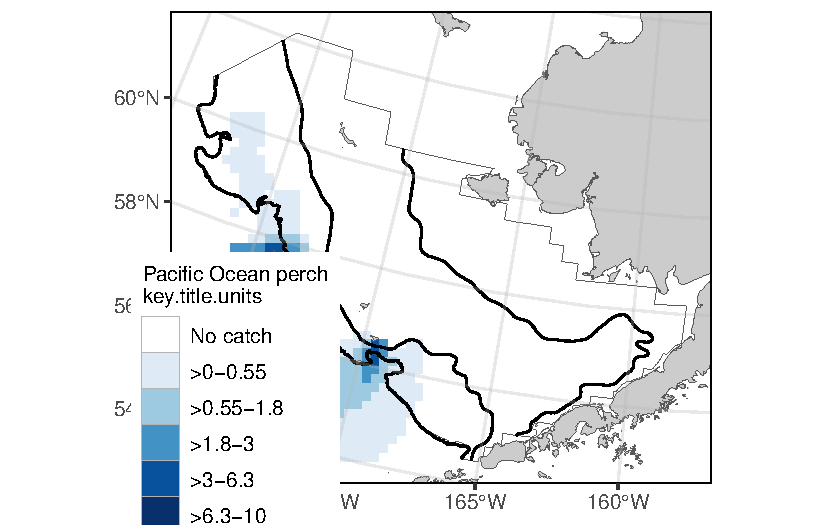
\includegraphics{content/akfin-oracle-sql-r_files/figure-pdf/test-6-fig-1.pdf}

}

\caption{Ex. 6: EBS Pacific Ocean perch CPUE and
\href{https://github.com/afsc-gap-products/akgfmaps}{\texttt{akgfmaps}}
map.}

\end{figure}

\hypertarget{access-api-data-using-r}{%
\chapter{Access API data using R}\label{access-api-data-using-r}}

Use the below function to pull AKFIN data through AKFIN's API.

\begin{Shaded}
\begin{Highlighting}[]
\CommentTok{\# load libraries}
\FunctionTok{library}\NormalTok{(dplyr)}
\FunctionTok{library}\NormalTok{(magrittr)}
\FunctionTok{library}\NormalTok{(httr)}
\FunctionTok{library}\NormalTok{(flextable)}

\CommentTok{\# tell R to not use scientific notation}
\FunctionTok{options}\NormalTok{(}\AttributeTok{scipen=}\DecValTok{999}\NormalTok{)}

\CommentTok{\# function for pulling data from the api using the httr package}
\NormalTok{get\_gap\_biomass}\OtherTok{\textless{}{-}}\ControlFlowTok{function}\NormalTok{(area\_id, species\_code) \{}
  \CommentTok{\# paste(... collapse=",") puts commas between vector elements}
\NormalTok{  area\_id }\OtherTok{\textless{}{-}} \FunctionTok{paste}\NormalTok{(area\_id, }\AttributeTok{collapse =} \StringTok{","}\NormalTok{)}
\NormalTok{  species\_code }\OtherTok{\textless{}{-}} \FunctionTok{paste}\NormalTok{(species\_code, }\AttributeTok{collapse =} \StringTok{","}\NormalTok{)}
  \CommentTok{\# httr code, parameters are after the \textquotesingle{}?\textquotesingle{}}
\NormalTok{  httr}\SpecialCharTok{::}\FunctionTok{content}\NormalTok{(}
\NormalTok{    httr}\SpecialCharTok{::}\FunctionTok{GET}\NormalTok{(}\FunctionTok{paste0}\NormalTok{(}\StringTok{"https://apex.psmfc.org/akfin/data\_marts/akmp/gap\_biomass?area\_id="}\NormalTok{,}
\NormalTok{                     area\_id,}
                     \StringTok{"\&species\_code="}\NormalTok{,}
\NormalTok{                     species\_code)),}
    \AttributeTok{type =} \StringTok{"application/json"}\NormalTok{) }\SpecialCharTok{\%\textgreater{}\%}
    \CommentTok{\# convert to data frame}
    \FunctionTok{bind\_rows}\NormalTok{()}
\NormalTok{\}}
\end{Highlighting}
\end{Shaded}

\hypertarget{ex.-1-load-lingcod-data}{%
\section{Ex. 1: Load lingcod data}\label{ex.-1-load-lingcod-data}}

\begin{Shaded}
\begin{Highlighting}[]
\NormalTok{lingcod\_biomass }\OtherTok{\textless{}{-}} \FunctionTok{get\_gap\_biomass}\NormalTok{(}\AttributeTok{area\_id=}\FunctionTok{c}\NormalTok{(}\DecValTok{40}\NormalTok{, }\DecValTok{41}\NormalTok{), }\AttributeTok{species\_code=}\DecValTok{21910}\NormalTok{)}
\NormalTok{flextable}\SpecialCharTok{::}\FunctionTok{flextable}\NormalTok{(}\FunctionTok{head}\NormalTok{(lingcod\_biomass)) }\SpecialCharTok{\%\textgreater{}\%}
\NormalTok{  flextable}\SpecialCharTok{::}\FunctionTok{theme\_zebra}\NormalTok{()}
\end{Highlighting}
\end{Shaded}

\part{Public Data (FOSS)}

The final, validated survey data are publicly accessible soon after
surveys are completed on the
\href{https://www.fisheries.noaa.gov/foss/}{Fisheries One Stop Shop
(FOSS) platform}. This data includes catch, haul, and environmental data
collected at each station. On the
\href{https://www.fisheries.noaa.gov/foss/}{FOSS data platform}, users
can interactively select, view, and download data. Descriptive
documentation and user-examples are available on the metadata page.

This data contains all of the catch, environmental, and haul data from
the fisheries-independent Groundfish and Shellfish Assessment Program
surveys in the Bering Sea, Aleutian Islands, and Gulf of Alaska. This
data is sought after by the general public, private entities, and NOAA
partners alike, including tribal organizations, K-12 classrooms,
academic institutions, for-profit groups, and non-profit groups. This
data is compiled and approved once a year after each summer survey
season and is available for open access.

\part{Collaborators and data users}

Below are a few packages and products currently using this data. If you
have developed a product, performed an analysis, or exhibited this data
in any way, reach out so we can showcase your hard work.

\begin{itemize}
\item
  \textbf{\href{https://apps-st.fisheries.noaa.gov/dismap}{NOAA
  Fisheries Distribution Mapping and Analysis Portal}};
  \emph{\href{https://www.fisheries.noaa.gov/contact/office-science-and-technology}{NOAA
  Fisheries Office of Science and Technology}}
\item
  \textbf{\href{https://pyafscgap.org/}{Pull data with python} and
  explore the
  \href{https://app.pyafscgap.org/\textquotesingle{}}{in-browser
  visualization tool}. Reference their
  \href{https://mybinder.org/v2/gh/SchmidtDSE/afscgap/main?urlpath=/tree/index.ipynb}{example
  Python notebook}}; \emph{\href{https://dse.berkeley.edu/}{The Eric and
  Wendy Schmidt Center for Data Science and the Environment at UC
  Berkeley}, including sam.pottinger@berkeley.edu,
  ccmartinez@berkeley.edu, gzarpellon@berkeley.edu, and
  kkoy@berkeley.edu.}
\end{itemize}

\hypertarget{cite-this-data-2}{%
\section*{Cite this data}\label{cite-this-data-2}}
\addcontentsline{toc}{section}{Cite this data}

\markright{Cite this data}

Use the below
\href{https://github.com/afsc-gap-products/gap_products/blob/main/code/CITATION_FOSSAFSCData.bib}{bibtext
citations}, as cited in our group's
\href{https://github.com/afsc-gap-products/citations/blob/main/cite/bibliography.bib}{citation
repository} for citing the data created and maintained in this repo
(NOAA Fisheries Alaska Fisheries Science Center, 2023). Add ``note =
\{Accessed: mm/dd/yyyy\}'' to append the day this data was accessed.

\begin{verbatim}
@misc{FOSSAFSCData,
  author = {{NOAA Fisheries Alaska Fisheries Science Center}},
  year = {2023}, 
  title = {Fisheries One Stop Shop Public Data: RACE Division Bottom Trawl Survey Data Query},
  howpublished = {https://www.fisheries.noaa.gov/foss},
  publisher = {{U.S. Dep. Commer.}},
  copyright = {Public Domain} 
}
\end{verbatim}

\hypertarget{data-description-4}{%
\chapter{Data description}\label{data-description-4}}

The Resource Assessment and Conservation Engineering Division (RACE)
Groundfish Assessment Program (GAP) of the Alaska Fisheries Science
Center (AFSC) conducts fisheries-independent bottom trawl surveys to
monitor the condition of the demersal fish and crab stocks of Alaska.
These data are developed to describe the temporal distribution and
abundance of commercially and ecologically important groundfish species,
examine the changes in the species composition of the fauna over time
and space, and describe the physical environment of the groundfish
habitat.

There are no legal restrictions on access to the data. They reside in
the public domain and can be freely distributed. Users must read and
fully comprehend the metadata prior to use. Data should not be used
beyond the limits of the source scale. Acknowledgement of NOAA, as the
source from which these data were obtained, in any publications and/or
other representations of these data, is suggested. These data are
compiled and approved annually after each summer survey season. The data
from previous years are unlikely to change substantially once published.

These data are zero-filled (presence and absence) observations from
surveys conducted on fishing vessels. These surveys monitor trends in
distribution and abundance of groundfish, crab, and bottom-dwelling
species in Alaska's marine ecosystems. These data include estimates of
catch-per-unit-effort (CPUE) for all identified species for index
stations. Some survey data are excluded, such as non-standard stations,
surveys completed in earlier years using different/non-standard gear,
and special tows and non-standard data collections.

Though not included in the public data, these surveys also collect
oceanographic and environmental data, and biological data such as
length, weight, stomach contents (to learn more about diet), otoliths
(fish ear bones to learn about age), and tissue samples for genetic
analysis, all of which can be shared upon special request. Also not
included in the public data are estimated biomass (average total weight
of all fish and crabs sampled) of crabs and groundfish that support the
creation of annual stock assessments.

\hypertarget{data-tables-2}{%
\section{Data tables}\label{data-tables-2}}

\hypertarget{foss_catch}{%
\subsection{FOSS\_CATCH}\label{foss_catch}}

These datasets, FOSS\_CATCH, FOSS\_CPUE\_PRESONLY, FOSS\_HAUL, and
FOSS\_SPECIES, when full joined by the HAULJOIN variable, includes
zero-filled (presence and absence) observations and
catch-per-unit-effort (CPUE) estimates for all identified species at for
index stations. These tables were created by the Resource Assessment and
Conservation Engineering Division (RACE) Groundfish Assessment Program
(GAP) of the Alaska Fisheries Science Center (AFSC). There are legal
restrictions on access to the data. These data are not intended for
public dissemination and should not be shared without the explicit
written consent of the data managers and owners (NOAA Fisheries). The
GitHub repository for the scripts that created this code can be found at
https://github.com/afsc-gap-products/gap\_products. For more information
about codes used in the tables, please refer to the survey code books
(https://www.fisheries.noaa.gov/resource/document/groundfish-survey-species-code-manual-and-data-codes-manual).
These data were last updated October 17, 2023.

Number of rows: 928,931

Number of columns: 7

Column name from data

Descriptive column Name

Units

Oracle data type

Column description

COUNT

Taxon count

count, whole number resolution

NUMBER(38,0)

Total whole number of individuals caught in haul.

CPUE\_KGKM2

Weight CPUE (kg/km2)

kilograms per kilometers squared

NUMBER(38,6)

Catch weight (kilograms) per unit effort (area swept by the net, units
square kilometers).

CPUE\_NOKM2

Number CPUE (no/km2)

count per kilometers squared

NUMBER(38,6)

Numerical catch per unit effort (area swept by the net, units square
kilometers).

HAULJOIN

Haul ID

ID code

NUMBER(38,0)

This is a unique numeric identifier assigned to each (vessel, cruise,
and haul) combination.

SPECIES\_CODE

Taxon code

ID code

NUMBER(38,0)

The species code of the organism associated with the `common\_name' and
`scientific\_name' columns. For a complete species list, review the
\href{https://www.fisheries.noaa.gov/resource/document/groundfish-survey-species-code-manual-and-data-codes-manual}{code
books}.

TAXON\_CONFIDENCE

Taxon confidence rating

category

VARCHAR2(255 BYTE)

Confidence in the ability of the survey team to correctly identify the
taxon to the specified level, based solely on identification skill
(e.g., not likelihood of a taxon being caught at that station on a
location-by-location basis). Quality codes follow: \textbf{`High'}: High
confidence and consistency. Taxonomy is stable and reliable at this
level, and field identification characteristics are well known and
reliable. \textbf{`Moderate'}: Moderate confidence. Taxonomy may be
questionable at this level, or field identification characteristics may
be variable and difficult to assess consistently. \textbf{`Low'}: Low
confidence. Taxonomy is incompletely known, or reliable field
identification characteristics are unknown. Documentation:
\href{http://apps-afsc.fisheries.noaa.gov/Publications/ProcRpt/PR2009-04.pdf}{Species
identification confidence in the eastern Bering Sea shelf survey
(1982-2008)},
\href{http://apps-afsc.fisheries.noaa.gov/Publications/ProcRpt/PR2014-05.pdf}{Species
identification confidence in the eastern Bering Sea slope survey
(1976-2010)}, and
\href{http://apps-afsc.fisheries.noaa.gov/Publications/ProcRpt/PR2014-01.pdf}{Species
identification confidence in the Gulf of Alaska and Aleutian Islands
surveys (1980-2011)}.

WEIGHT\_KG

Sample or taxon weight (kg)

kilograms

NUMBER(38,3)

Weight (thousandths of a kilogram) of individuals in a haul by taxon.

\hypertarget{foss_cpue_presonly}{%
\subsection{FOSS\_CPUE\_PRESONLY}\label{foss_cpue_presonly}}

These datasets, FOSS\_CATCH, FOSS\_CPUE\_PRESONLY, FOSS\_HAUL, and
FOSS\_SPECIES, when full joined by the HAULJOIN variable, includes
zero-filled (presence and absence) observations and
catch-per-unit-effort (CPUE) estimates for all identified species at for
index stations. These tables were created by the Resource Assessment and
Conservation Engineering Division (RACE) Groundfish Assessment Program
(GAP) of the Alaska Fisheries Science Center (AFSC). There are legal
restrictions on access to the data. These data are not intended for
public dissemination and should not be shared without the explicit
written consent of the data managers and owners (NOAA Fisheries). The
GitHub repository for the scripts that created this code can be found at
https://github.com/afsc-gap-products/gap\_products. For more information
about codes used in the tables, please refer to the survey code books
(https://www.fisheries.noaa.gov/resource/document/groundfish-survey-species-code-manual-and-data-codes-manual).
These data were last updated October 17, 2023.

Number of rows: 928,931

Number of columns: 38

Column name from data

Descriptive column Name

Units

Oracle data type

Column description

AREA\_SWEPT\_KM2

Area swept (km)

kilometers

NUMBER(38,6)

The area the net covered while the net was fishing (kilometers squared),
defined as the distance fished times the net width.

BOTTOM\_TEMPERATURE\_C

Bottom temperature (degrees celsius)

degrees Celsius

NUMBER(38,1)

Bottom temperature (tenths of a degree Celsius); NA indicates removed or
missing values.

COMMON\_NAME

Taxon common name

text

VARCHAR2(255 BYTE)

The common name of the marine organism associated with the
`scientific\_name' and `species\_code' columns. For a complete species
list, review the
\href{https://www.fisheries.noaa.gov/resource/document/groundfish-survey-species-code-manual-and-data-codes-manual}{code
books}.

COUNT

Taxon count

count, whole number resolution

NUMBER(38,0)

Total whole number of individuals caught in haul.

CPUE\_KGKM2

Weight CPUE (kg/km2)

kilograms per kilometers squared

NUMBER(38,6)

Catch weight (kilograms) per unit effort (area swept by the net, units
square kilometers).

CPUE\_NOKM2

Number CPUE (no/km2)

count per kilometers squared

NUMBER(38,6)

Numerical catch per unit effort (area swept by the net, units square
kilometers).

CRUISE

Cruise ID

ID code

NUMBER(38,0)

This is a six-digit integer identifying the cruise number of the form:
YYYY99 (where YYYY = year of the cruise; 99 = 2-digit number and is
sequential; 01 denotes the first cruise that vessel made in this year,
02 is the second, etc.).

CRUISEJOIN

Cruise ID

ID code

NUMBER(38,0)

Unique interger ID assigned to each survey, vessel, and year
combination.

DATE\_TIME

Date and time

MM/DD/YYYY HH::MM

DATE

The date (MM/DD/YYYY) and time (HH:MM) of the haul.

DEPTH\_M

Depth (m)

degrees Celsius

NUMBER(38,1)

Bottom depth (meters).

DISTANCE\_FISHED\_KM

Distance fished (km)

degrees Celsius

NUMBER(38,3)

Distance the net fished (thousandths of kilometers).

DURATION\_HR

Tow duration (decimal hr)

hours

NUMBER(38,1)

This is the elapsed time between start and end of a haul (decimal
hours).

HAUL

Haul number

ID code

NUMBER(38,0)

This number uniquely identifies a sampling event (haul) within a cruise.
It is a sequential number, in chronological order of occurrence.

HAULJOIN

Haul ID

ID code

NUMBER(38,0)

This is a unique numeric identifier assigned to each (vessel, cruise,
and haul) combination.

ID\_RANK

Lowest taxonomic rank

text

VARCHAR2(255 BYTE)

Lowest taxonomic rank of a given species entry.

ITIS

ITIS taxonomic serial number

ID code

NUMBER(38,0)

Species code as identified in the Integrated Taxonomic Information
System (https://itis.gov/).

LATITUDE\_DD\_END

End latitude (decimal degrees)

decimal degrees

NUMBER(38,6)

Latitude (one hundred thousandth of a decimal degree) of the end of the
haul.

LATITUDE\_DD\_START

Start latitude (decimal degrees)

decimal degrees

NUMBER(38,6)

Latitude (one hundred thousandth of a decimal degree) of the start of
the haul.

LONGITUDE\_DD\_END

End longitude (decimal degrees)

decimal degrees

NUMBER(38,6)

Longitude (one hundred thousandth of a decimal degree) of the end of the
haul.

LONGITUDE\_DD\_START

Start longitude (decimal degrees)

decimal degrees

NUMBER(38,6)

Longitude (one hundred thousandth of a decimal degree) of the start of
the haul.

NET\_HEIGHT\_M

Net height (m)

meters

NUMBER(38,1)

Measured or estimated distance (meters) between footrope and headrope of
the trawl.

NET\_WIDTH\_M

Net width (m)

meters

NUMBER(38,1)

Measured or estimated distance (meters) between wingtips of the trawl.

PERFORMANCE

Haul performance code

category

NUMBER(38,0)

This denotes what, if any, issues arose during the haul. For more
information, review the
\href{https://www.fisheries.noaa.gov/resource/document/groundfish-survey-species-code-manual-and-data-codes-manual}{code
books}.

SCIENTIFIC\_NAME

Taxon scientific name

text

VARCHAR2(255 BYTE)

The scientific name of the organism associated with the `common\_name'
and `species\_code' columns. For a complete taxon list, review the
\href{https://www.fisheries.noaa.gov/resource/document/groundfish-survey-species-code-manual-and-data-codes-manual}{code
books}.

SPECIES\_CODE

Taxon code

ID code

NUMBER(38,0)

The species code of the organism associated with the `common\_name' and
`scientific\_name' columns. For a complete species list, review the
\href{https://www.fisheries.noaa.gov/resource/document/groundfish-survey-species-code-manual-and-data-codes-manual}{code
books}.

SRVY

Survey

text abbreviated

VARCHAR2(255 BYTE)

Abbreviated survey names. The column `srvy' is associated with the
`survey' and `survey\_id' columns. Northern Bering Sea (NBS),
Southeastern Bering Sea (EBS), Bering Sea Slope (BSS), Gulf of Alaska
(GOA), Aleutian Islands (AI).

STATION

Station ID

ID code

VARCHAR2(255 BYTE)

Alpha-numeric designation for the station established in the design of a
survey.

STRATUM

Stratum ID

ID code

NUMBER(10,0)

RACE database statistical area for analyzing data. Strata were designed
using bathymetry and other geographic and habitat-related elements. The
strata are unique to each survey region. Stratum of value 0 indicates
experimental tows.

SURFACE\_TEMPERATURE\_C

Surface temperature (Degrees Celsius)

degrees Celsius

NUMBER(38,1)

Surface temperature (tenths of a degree Celsius); NA indicates removed
or missing values.

SURVEY

Survey Name

text

VARCHAR2(255 BYTE)

Name and description of survey. The column `survey' is associated with
the `srvy' and `survey\_id' columns.

SURVEY\_DEFINITION\_ID

Survey ID

ID code

NUMBER(38,0)

This number uniquely identifies a survey. Name and description of
survey. The column `survey\_id' is associated with the `srvy' and
`survey' columns. For a complete list of surveys, review the
\href{https://www.fisheries.noaa.gov/resource/document/groundfish-survey-species-code-manual-and-data-codes-manual}{code
books}.

SURVEY\_NAME

NA

NA

NA

NA

TAXON\_CONFIDENCE

Taxon confidence rating

category

VARCHAR2(255 BYTE)

Confidence in the ability of the survey team to correctly identify the
taxon to the specified level, based solely on identification skill
(e.g., not likelihood of a taxon being caught at that station on a
location-by-location basis). Quality codes follow: \textbf{`High'}: High
confidence and consistency. Taxonomy is stable and reliable at this
level, and field identification characteristics are well known and
reliable. \textbf{`Moderate'}: Moderate confidence. Taxonomy may be
questionable at this level, or field identification characteristics may
be variable and difficult to assess consistently. \textbf{`Low'}: Low
confidence. Taxonomy is incompletely known, or reliable field
identification characteristics are unknown. Documentation:
\href{http://apps-afsc.fisheries.noaa.gov/Publications/ProcRpt/PR2009-04.pdf}{Species
identification confidence in the eastern Bering Sea shelf survey
(1982-2008)},
\href{http://apps-afsc.fisheries.noaa.gov/Publications/ProcRpt/PR2014-05.pdf}{Species
identification confidence in the eastern Bering Sea slope survey
(1976-2010)}, and
\href{http://apps-afsc.fisheries.noaa.gov/Publications/ProcRpt/PR2014-01.pdf}{Species
identification confidence in the Gulf of Alaska and Aleutian Islands
surveys (1980-2011)}.

VESSEL\_ID

Vessel ID

ID code

NUMBER(38,0)

ID number of the vessel used to collect data for that haul. The column
`vessel\_id' is associated with the `vessel\_name' column. Note that it
is possible for a vessel to have a new name but the same vessel id
number. For a complete list of vessel ID codes, review the
\href{https://www.fisheries.noaa.gov/resource/document/groundfish-survey-species-code-manual-and-data-codes-manual}{code
books}.

VESSEL\_NAME

Vessel name

text

VARCHAR2(255 BYTE)

Name of the vessel used to collect data for that haul. The column
`vessel\_name' is associated with the `vessel\_id' column. Note that it
is possible for a vessel to have a new name but the same vessel id
number. For a complete list of vessel ID codes, review the
\href{https://www.fisheries.noaa.gov/resource/document/groundfish-survey-species-code-manual-and-data-codes-manual}{code
books}.

WEIGHT\_KG

Sample or taxon weight (kg)

kilograms

NUMBER(38,3)

Weight (thousandths of a kilogram) of individuals in a haul by taxon.

WORMS

World Register of Marine Species Taxonomic Serial Number

ID code

NUMBER(38,0)

Species code as identified in the World Register of Marine Species
(WoRMS) (https://www.marinespecies.org/).

YEAR

Survey year

year

NUMBER(10,0)

Year the observation (survey) was collected.

\hypertarget{foss_haul}{%
\subsection{FOSS\_HAUL}\label{foss_haul}}

These datasets, FOSS\_CATCH, FOSS\_CPUE\_PRESONLY, FOSS\_HAUL, and
FOSS\_SPECIES, when full joined by the HAULJOIN variable, includes
zero-filled (presence and absence) observations and
catch-per-unit-effort (CPUE) estimates for all identified species at for
index stations. These tables were created by the Resource Assessment and
Conservation Engineering Division (RACE) Groundfish Assessment Program
(GAP) of the Alaska Fisheries Science Center (AFSC). There are legal
restrictions on access to the data. These data are not intended for
public dissemination and should not be shared without the explicit
written consent of the data managers and owners (NOAA Fisheries). The
GitHub repository for the scripts that created this code can be found at
https://github.com/afsc-gap-products/gap\_products. For more information
about codes used in the tables, please refer to the survey code books
(https://www.fisheries.noaa.gov/resource/document/groundfish-survey-species-code-manual-and-data-codes-manual).
These data were last updated October 17, 2023.

Number of rows: 32,626

Number of columns: 27

Column name from data

Descriptive column Name

Units

Oracle data type

Column description

AREA\_SWEPT\_KM2

Area swept (km)

kilometers

NUMBER(38,6)

The area the net covered while the net was fishing (kilometers squared),
defined as the distance fished times the net width.

BOTTOM\_TEMPERATURE\_C

Bottom temperature (degrees celsius)

degrees Celsius

NUMBER(38,1)

Bottom temperature (tenths of a degree Celsius); NA indicates removed or
missing values.

CRUISE

Cruise ID

ID code

NUMBER(38,0)

This is a six-digit integer identifying the cruise number of the form:
YYYY99 (where YYYY = year of the cruise; 99 = 2-digit number and is
sequential; 01 denotes the first cruise that vessel made in this year,
02 is the second, etc.).

CRUISEJOIN

Cruise ID

ID code

NUMBER(38,0)

Unique interger ID assigned to each survey, vessel, and year
combination.

DATE\_TIME

Date and time

MM/DD/YYYY HH::MM

DATE

The date (MM/DD/YYYY) and time (HH:MM) of the haul.

DEPTH\_M

Depth (m)

degrees Celsius

NUMBER(38,1)

Bottom depth (meters).

DISTANCE\_FISHED\_KM

Distance fished (km)

degrees Celsius

NUMBER(38,3)

Distance the net fished (thousandths of kilometers).

DURATION\_HR

Tow duration (decimal hr)

hours

NUMBER(38,1)

This is the elapsed time between start and end of a haul (decimal
hours).

HAUL

Haul number

ID code

NUMBER(38,0)

This number uniquely identifies a sampling event (haul) within a cruise.
It is a sequential number, in chronological order of occurrence.

HAULJOIN

Haul ID

ID code

NUMBER(38,0)

This is a unique numeric identifier assigned to each (vessel, cruise,
and haul) combination.

LATITUDE\_DD\_END

End latitude (decimal degrees)

decimal degrees

NUMBER(38,6)

Latitude (one hundred thousandth of a decimal degree) of the end of the
haul.

LATITUDE\_DD\_START

Start latitude (decimal degrees)

decimal degrees

NUMBER(38,6)

Latitude (one hundred thousandth of a decimal degree) of the start of
the haul.

LONGITUDE\_DD\_END

End longitude (decimal degrees)

decimal degrees

NUMBER(38,6)

Longitude (one hundred thousandth of a decimal degree) of the end of the
haul.

LONGITUDE\_DD\_START

Start longitude (decimal degrees)

decimal degrees

NUMBER(38,6)

Longitude (one hundred thousandth of a decimal degree) of the start of
the haul.

NET\_HEIGHT\_M

Net height (m)

meters

NUMBER(38,1)

Measured or estimated distance (meters) between footrope and headrope of
the trawl.

NET\_WIDTH\_M

Net width (m)

meters

NUMBER(38,1)

Measured or estimated distance (meters) between wingtips of the trawl.

PERFORMANCE

Haul performance code

category

NUMBER(38,0)

This denotes what, if any, issues arose during the haul. For more
information, review the
\href{https://www.fisheries.noaa.gov/resource/document/groundfish-survey-species-code-manual-and-data-codes-manual}{code
books}.

SRVY

Survey

text abbreviated

VARCHAR2(255 BYTE)

Abbreviated survey names. The column `srvy' is associated with the
`survey' and `survey\_id' columns. Northern Bering Sea (NBS),
Southeastern Bering Sea (EBS), Bering Sea Slope (BSS), Gulf of Alaska
(GOA), Aleutian Islands (AI).

STATION

Station ID

ID code

VARCHAR2(255 BYTE)

Alpha-numeric designation for the station established in the design of a
survey.

STRATUM

Stratum ID

ID code

NUMBER(10,0)

RACE database statistical area for analyzing data. Strata were designed
using bathymetry and other geographic and habitat-related elements. The
strata are unique to each survey region. Stratum of value 0 indicates
experimental tows.

SURFACE\_TEMPERATURE\_C

Surface temperature (Degrees Celsius)

degrees Celsius

NUMBER(38,1)

Surface temperature (tenths of a degree Celsius); NA indicates removed
or missing values.

SURVEY

Survey Name

text

VARCHAR2(255 BYTE)

Name and description of survey. The column `survey' is associated with
the `srvy' and `survey\_id' columns.

SURVEY\_DEFINITION\_ID

Survey ID

ID code

NUMBER(38,0)

This number uniquely identifies a survey. Name and description of
survey. The column `survey\_id' is associated with the `srvy' and
`survey' columns. For a complete list of surveys, review the
\href{https://www.fisheries.noaa.gov/resource/document/groundfish-survey-species-code-manual-and-data-codes-manual}{code
books}.

SURVEY\_NAME

NA

NA

NA

NA

VESSEL\_ID

Vessel ID

ID code

NUMBER(38,0)

ID number of the vessel used to collect data for that haul. The column
`vessel\_id' is associated with the `vessel\_name' column. Note that it
is possible for a vessel to have a new name but the same vessel id
number. For a complete list of vessel ID codes, review the
\href{https://www.fisheries.noaa.gov/resource/document/groundfish-survey-species-code-manual-and-data-codes-manual}{code
books}.

VESSEL\_NAME

Vessel name

text

VARCHAR2(255 BYTE)

Name of the vessel used to collect data for that haul. The column
`vessel\_name' is associated with the `vessel\_id' column. Note that it
is possible for a vessel to have a new name but the same vessel id
number. For a complete list of vessel ID codes, review the
\href{https://www.fisheries.noaa.gov/resource/document/groundfish-survey-species-code-manual-and-data-codes-manual}{code
books}.

YEAR

Survey year

year

NUMBER(10,0)

Year the observation (survey) was collected.

\hypertarget{foss_species}{%
\subsection{FOSS\_SPECIES}\label{foss_species}}

These datasets, FOSS\_CATCH, FOSS\_CPUE\_PRESONLY, FOSS\_HAUL, and
FOSS\_SPECIES, when full joined by the HAULJOIN variable, includes
zero-filled (presence and absence) observations and
catch-per-unit-effort (CPUE) estimates for all identified species at for
index stations. These tables were created by the Resource Assessment and
Conservation Engineering Division (RACE) Groundfish Assessment Program
(GAP) of the Alaska Fisheries Science Center (AFSC). There are legal
restrictions on access to the data. These data are not intended for
public dissemination and should not be shared without the explicit
written consent of the data managers and owners (NOAA Fisheries). The
GitHub repository for the scripts that created this code can be found at
https://github.com/afsc-gap-products/gap\_products. For more information
about codes used in the tables, please refer to the survey code books
(https://www.fisheries.noaa.gov/resource/document/groundfish-survey-species-code-manual-and-data-codes-manual).
These data were last updated October 17, 2023.

Number of rows: 1,936

Number of columns: 6

Column name from data

Descriptive column Name

Units

Oracle data type

Column description

COMMON\_NAME

Taxon common name

text

VARCHAR2(255 BYTE)

The common name of the marine organism associated with the
`scientific\_name' and `species\_code' columns. For a complete species
list, review the
\href{https://www.fisheries.noaa.gov/resource/document/groundfish-survey-species-code-manual-and-data-codes-manual}{code
books}.

ID\_RANK

Lowest taxonomic rank

text

VARCHAR2(255 BYTE)

Lowest taxonomic rank of a given species entry.

ITIS

ITIS taxonomic serial number

ID code

NUMBER(38,0)

Species code as identified in the Integrated Taxonomic Information
System (https://itis.gov/).

SCIENTIFIC\_NAME

Taxon scientific name

text

VARCHAR2(255 BYTE)

The scientific name of the organism associated with the `common\_name'
and `species\_code' columns. For a complete taxon list, review the
\href{https://www.fisheries.noaa.gov/resource/document/groundfish-survey-species-code-manual-and-data-codes-manual}{code
books}.

SPECIES\_CODE

Taxon code

ID code

NUMBER(38,0)

The species code of the organism associated with the `common\_name' and
`scientific\_name' columns. For a complete species list, review the
\href{https://www.fisheries.noaa.gov/resource/document/groundfish-survey-species-code-manual-and-data-codes-manual}{code
books}.

WORMS

World Register of Marine Species Taxonomic Serial Number

ID code

NUMBER(38,0)

Species code as identified in the World Register of Marine Species
(WoRMS) (https://www.marinespecies.org/).

\hypertarget{foss_survey_species}{%
\subsection{FOSS\_SURVEY\_SPECIES}\label{foss_survey_species}}

This reference dataset contains the full list of species by survey to be
used to zero-fill FOSS\_CATCH and FOSS\_HAUL for each survey. These
tables were created by the Resource Assessment and Conservation
Engineering Division (RACE) Groundfish Assessment Program (GAP) of the
Alaska Fisheries Science Center (AFSC). There are legal restrictions on
access to the data. These data are not intended for public dissemination
and should not be shared without the explicit written consent of the
data managers and owners (NOAA Fisheries). The GitHub repository for the
scripts that created this code can be found at
https://github.com/afsc-gap-products/gap\_products. For more information
about codes used in the tables, please refer to the survey code books
(https://www.fisheries.noaa.gov/resource/document/groundfish-survey-species-code-manual-and-data-codes-manual).
These data were last updated October 17, 2023.

Number of rows: 5,025

Number of columns: 2

Column name from data

Descriptive column Name

Units

Oracle data type

Column description

SPECIES\_CODE

Taxon code

ID code

NUMBER(38,0)

The species code of the organism associated with the `common\_name' and
`scientific\_name' columns. For a complete species list, review the
\href{https://www.fisheries.noaa.gov/resource/document/groundfish-survey-species-code-manual-and-data-codes-manual}{code
books}.

SURVEY\_DEFINITION\_ID

Survey ID

ID code

NUMBER(38,0)

This number uniquely identifies a survey. Name and description of
survey. The column `survey\_id' is associated with the `srvy' and
`survey' columns. For a complete list of surveys, review the
\href{https://www.fisheries.noaa.gov/resource/document/groundfish-survey-species-code-manual-and-data-codes-manual}{code
books}.

\hypertarget{foss_taxon_group}{%
\subsection{FOSS\_TAXON\_GROUP}\label{foss_taxon_group}}

This reference dataset contains suggested search groups for simplifying
species selection in the FOSS data platform so users can better search
through FOSS\_CATCH. These tables were created by the Resource
Assessment and Conservation Engineering Division (RACE) Groundfish
Assessment Program (GAP) of the Alaska Fisheries Science Center (AFSC).
There are legal restrictions on access to the data. These data are not
intended for public dissemination and should not be shared without the
explicit written consent of the data managers and owners (NOAA
Fisheries). The GitHub repository for the scripts that created this code
can be found at https://github.com/afsc-gap-products/gap\_products. For
more information about codes used in the tables, please refer to the
survey code books
(https://www.fisheries.noaa.gov/resource/document/groundfish-survey-species-code-manual-and-data-codes-manual).
These data were last updated October 17, 2023.

Number of rows: 37,606

Number of columns: 3

Column name from data

Descriptive column Name

Units

Oracle data type

Column description

CLASSIFICATION

Taxonomic classification rank group

category

VARCHAR2(255 BYTE)

Phylogenetic classification group rank for a given species.

RANK\_ID

Taxonomic rank

category

VARCHAR2(255 BYTE)

The taxonomic rank of a taxon identification.

SPECIES\_CODE

Taxon code

ID code

NUMBER(38,0)

The species code of the organism associated with the `common\_name' and
`scientific\_name' columns. For a complete species list, review the
\href{https://www.fisheries.noaa.gov/resource/document/groundfish-survey-species-code-manual-and-data-codes-manual}{code
books}.

\hypertarget{using-the-foss-platform}{%
\chapter{Using the FOSS platform}\label{using-the-foss-platform}}

\begin{figure}

{\centering 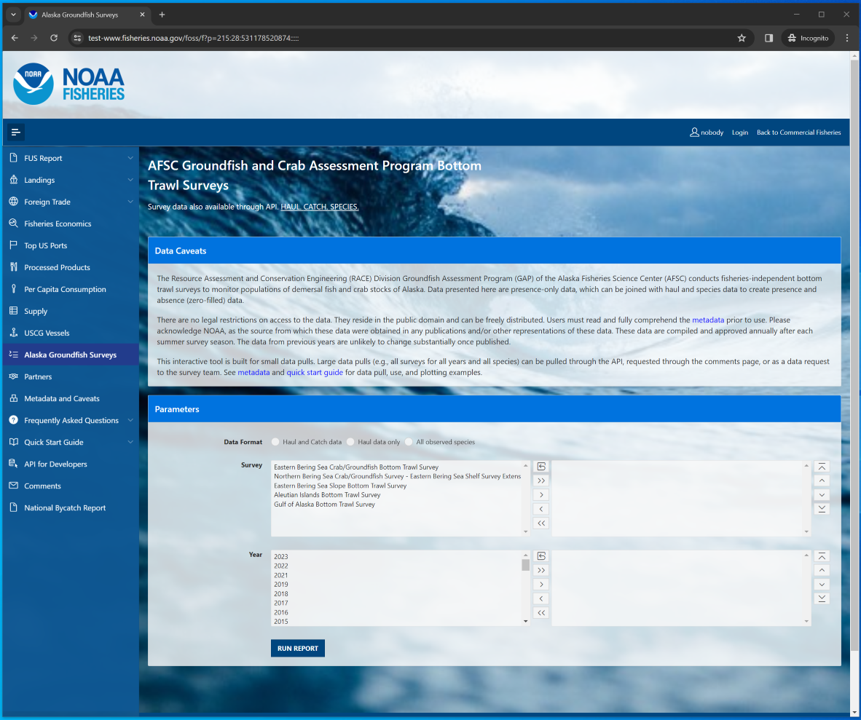
\includegraphics[width=6.24in,height=\textheight]{content/../img/foss_1_interface.png}

}

\caption{AFSC Groundfish and Crab Assessment Program Bottom Trawl Survey
data interface on the Fisheries One Stop Shop platform.}

\end{figure}

\hypertarget{select-and-filter}{%
\section{Select and filter}\label{select-and-filter}}

Select, filter, and package this and other NOAA Fisheries data from the
\href{https://www.fisheries.noaa.gov/foss}{Fisheries One Stop Shop
(FOSS)} platform. A user guide for the FOSS platform can be found
\href{https://www.fisheries.noaa.gov/foss/f?p=215:7:7542600605674:::::}{here}.
To begin a report, select options from the boxes what you need data for.

For a given box, select one or a few options from the ``options box''
(list on the left) to query by highlighting them. To select multiple
options, hold down the CTRL key while clicking on the options of
interest, or click and drag down the list. Once the options you wish to
be included in your query are highlighted, click the right-pointing
arrow (\texttt{\textgreater{}}) to move them into the ``selection box''
(list on the right). If you accidentally select an option that you do
not want to query, simply select the unwanted option from the selection
box and click the left-pointing arrow (\texttt{\textless{}}).

If you wish to select all options from the options box and send them to
the selection box, simply click the double right-pointing arrow
(\texttt{\textgreater{}\textgreater{}}). If you want to unselect all
options from the selection box, use the double left-pointing arrow
(\texttt{\textless{}\textless{}}) or the reset icon.

To find a specific species or group more quickly you can use the
\texttt{Search\ Species} option to quickly narrow the options. Search
for parts of species common names in the \texttt{Search\ Species} box by
entering a term and clicking the \texttt{search} button. The platform
will return a shorter list in the \texttt{Speices} options box of only
species that contain a match to that search term.

Use the \texttt{Reset\ All\ Parameters} button to reset all parameters
for entire form.

\begin{figure}

{\centering 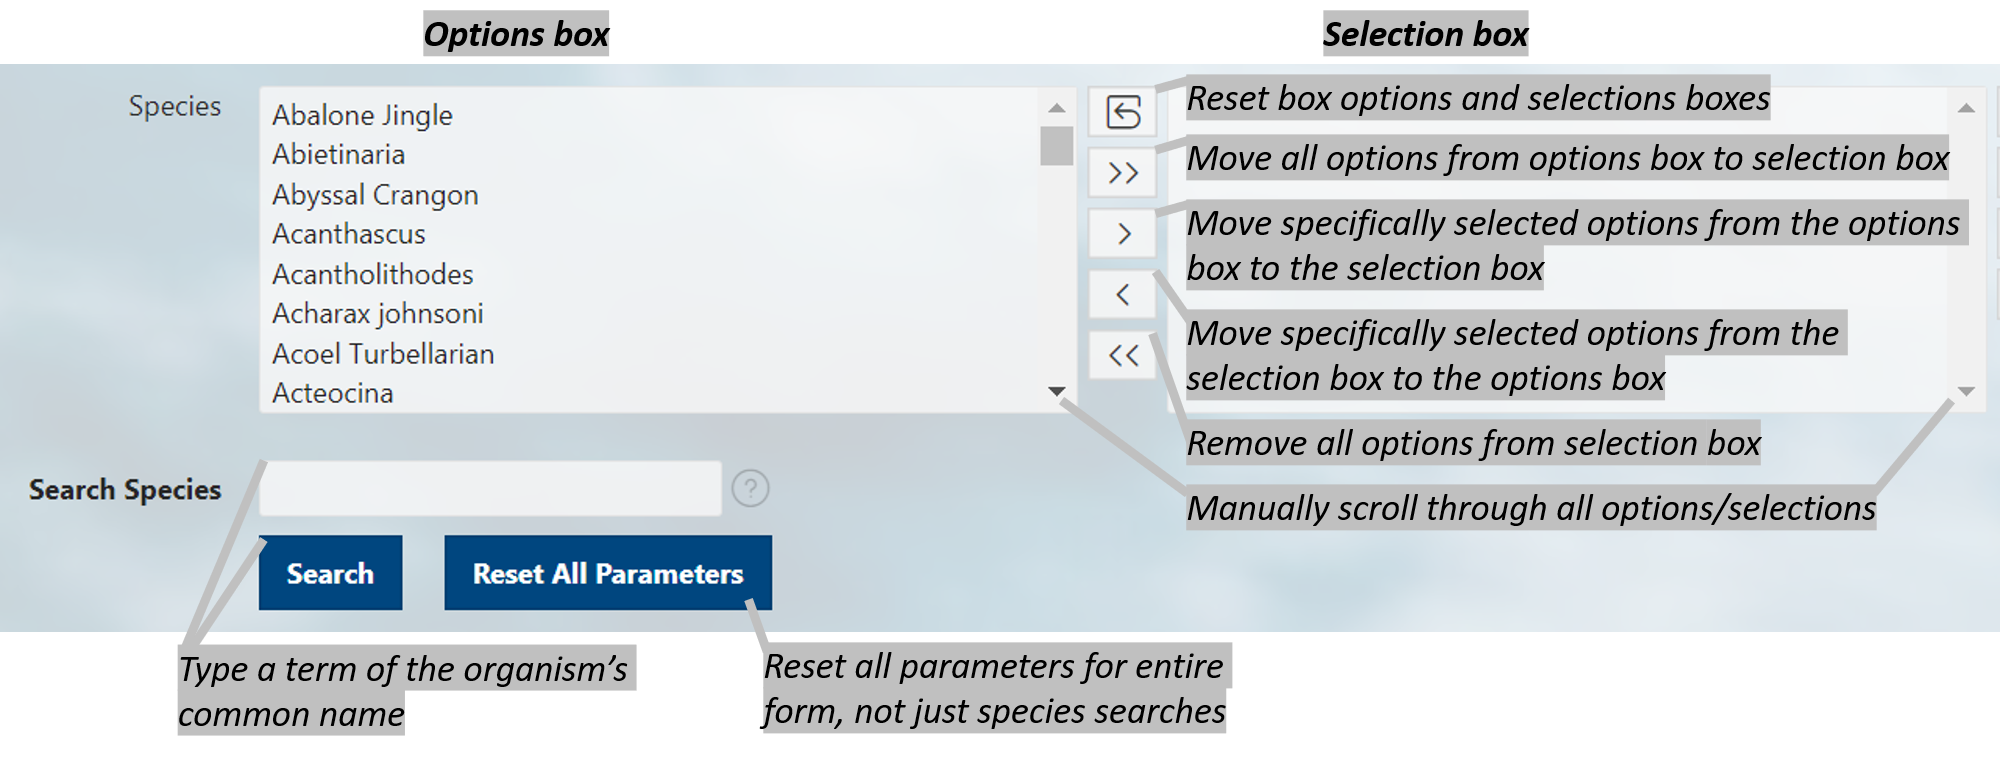
\includegraphics[width=6.67in,height=\textheight]{content/../img/foss_2_select.png}

}

\caption{Diagram of selection and search tools available on the FOSS
platofrom.}

\end{figure}

Filter options:

\begin{itemize}
\tightlist
\item
  \texttt{Survey}: Each survey has different in design, time series, and
  history. More information on each survey and their designs can be
  found in our
  \href{https://www.fisheries.noaa.gov/alaska/science-data/groundfish-assessment-program-bottom-trawl-surveys\#data-products}{annual
  data reports}.
\item
  \texttt{Year}: Surveys are not conducted in all years, so only data
  from the years for which the survey was conducted will be returned.
\item
  \texttt{Species}: Common name of all species ever encountered in the
  survey. Find more information about these species in our
  \href{https://www.fisheries.noaa.gov/resource/document/groundfish-survey-species-code-manual-and-data-codes-manual}{survey
  code books}.
\end{itemize}

\begin{quote}
In this example, we'll select for 2022 eastern Bering Sea Pacific cod
data. Here, we used the \texttt{Search\ Species} box to search for
species with the term ``cod'' in their common names and selected
``Pacific cod'' from that shortened list.
\end{quote}

\begin{figure}

{\centering 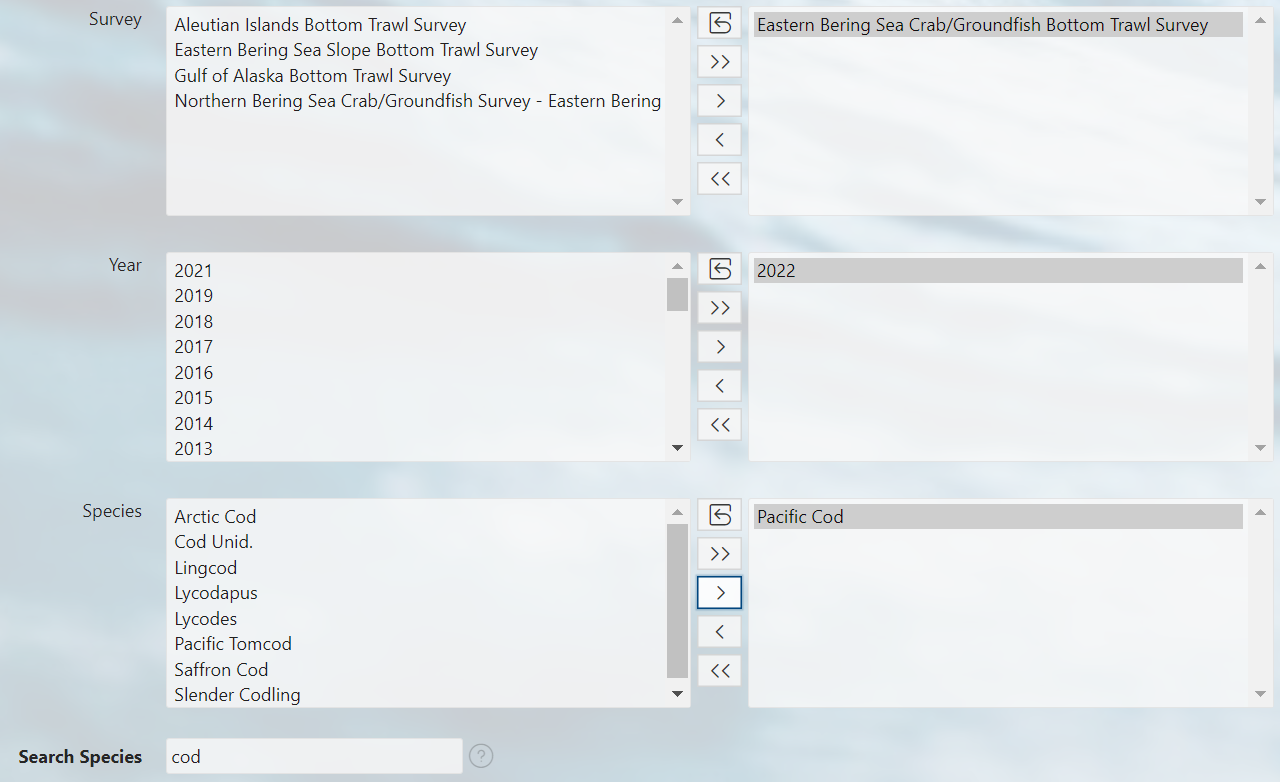
\includegraphics[width=4.27in,height=\textheight]{content/../img/foss_3_selected.png}

}

\caption{Diagram of selection and search tools available on the FOSS
platofrom.}

\end{figure}

\hypertarget{select-data-format}{%
\section{Select data format}\label{select-data-format}}

Select from the below radio list of pre-designed output tables. Once you
run the report, the user can further specify filter data and select
columns of interest. The tables below will only include data from the
selections made in the previous step.

\begin{itemize}
\tightlist
\item
  \texttt{All\ Data\ Fields:\ Presence\ and\ Absence\ (zero-filled)}:
  The most complete version of the data, including species, catch, haul,
  and environmental data. This data will include catch data for where
  species were caught and zeros for where the species were not caught.
  This is important for calculating catch-per-unit-effort data,
  preparing distribution plots (e.g.,
  \href{https://github.com/afsc-gap-products/akgfmaps}{using the
  akgfmaps R package}), and many statistical analyses.
\item
  \texttt{All\ Data\ Fields:\ Presence-only\ (non-zero)}: The second
  most complete version of the data, including species, catch, haul, and
  environmental data. However, this data only includes catch data for
  where species were caught and does not include zeros for where the
  species were not caught. This will return smaller, more focused data
  and can be useful for quickly assessing how many species were caught
  or how many stations species were caught at.
\item
  \texttt{Catch\ data:\ Presence\ and\ Absence\ (zero-filled)}: This
  data set is similar to
  \texttt{All\ Data\ Fields:\ Presence\ and\ Absence\ (zero-filled)},
  but only includes catch and species data columns.
\item
  \texttt{Catch\ data:\ Presence-only\ (non-zero)}: This data set is
  similar to \texttt{All\ Data\ Fields:\ Presence-only\ (non-zero)}, but
  only includes catch and species data columns.
\item
  \texttt{Haul\ Data}: This data set only includes haul and
  environmental data collected from the survey. This data will only
  include one observation per haul event/station.
\end{itemize}

\begin{quote}
In this example, we'll select
\texttt{All\ Data\ Fields:\ Presence\ and\ Absence\ (zero-filled).}
\end{quote}

\begin{figure}

{\centering 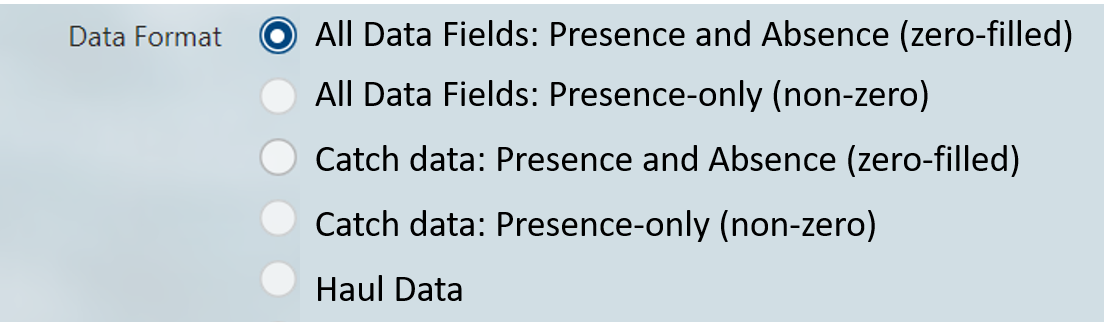
\includegraphics[width=3.68in,height=\textheight]{content/../img/foss_4_data_format.png}

}

\caption{Diagram of the pre-set data format options.}

\end{figure}

\hypertarget{run-report}{%
\section{Run report}\label{run-report}}

Click the \texttt{RUN\ REPORT} button. Below the select and filter area,
the results of your query will appear below the page in the format you
selected. To change the format, make a different selection and run the
report again. Further modifications to your results can be made by
clicking on the \texttt{Actions} button above your data. Here you can
\texttt{download} your data, \texttt{select\ columns} included in your
results, and apply a variety of \texttt{filters} and mathematical tools.

\begin{figure}

{\centering 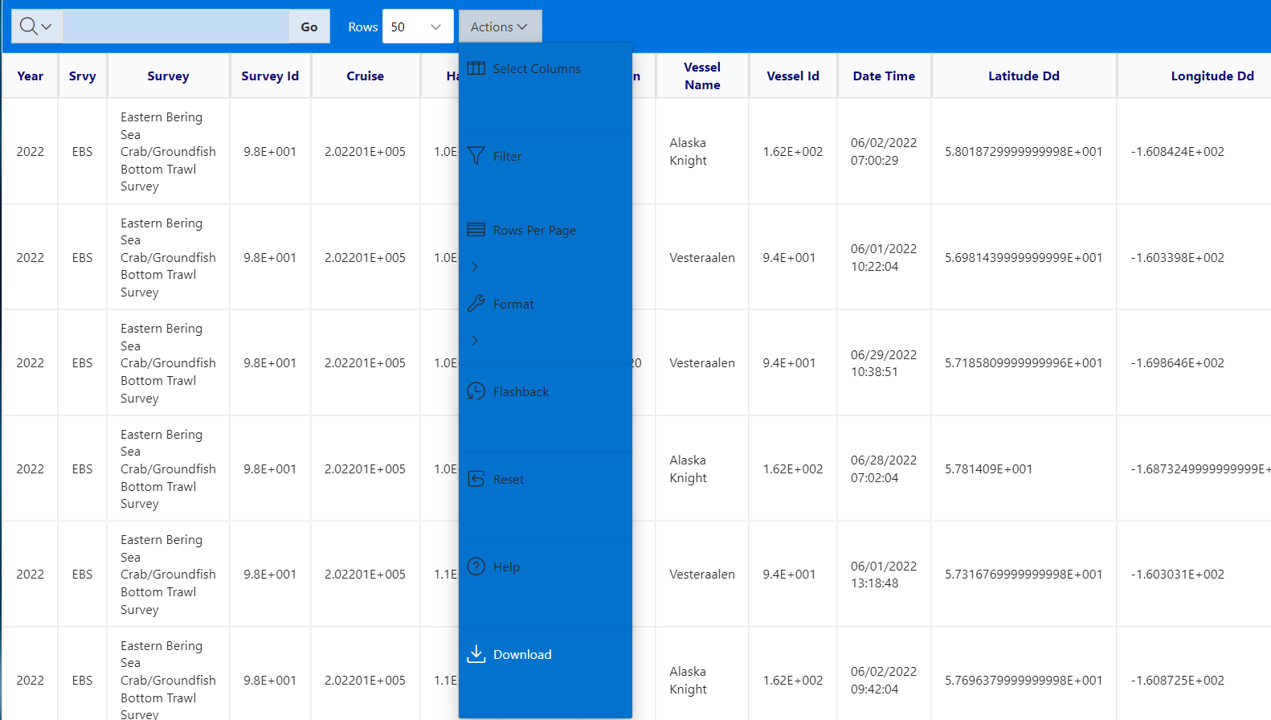
\includegraphics[width=4.24in,height=\textheight]{content/../img/foss_5_run_report.png}

}

\caption{Example data returned from running the report.}

\end{figure}

\hypertarget{access-via-api-and-r}{%
\chapter{Access via API and R}\label{access-via-api-and-r}}

An application programming interface (API) is a way for two or more
computer programs to communicate with each other.

More information about how to amend API links can be found
\href{https://docs.oracle.com/en/database/oracle/oracle-rest-data-services/22.3/books.html\#AELIG90103/}{here}.
Useful introductions to using APIs in \texttt{R} can be found
\href{https://www.dataquest.io/blog/r-api-tutorial/}{here}.

\hypertarget{ex.-1-load-the-first-25-rows-default-of-data}{%
\section{Ex. 1: Load the first 25 rows (default) of
data}\label{ex.-1-load-the-first-25-rows-default-of-data}}

\begin{Shaded}
\begin{Highlighting}[]
 \CommentTok{\# install.packages(c("httr", "jsonlite"))}
\FunctionTok{library}\NormalTok{(httr)}
\FunctionTok{library}\NormalTok{(jsonlite)}
\FunctionTok{library}\NormalTok{(dplyr)}

 \CommentTok{\# link to the API}
\NormalTok{api\_link }\OtherTok{\textless{}{-}} \StringTok{"https://apps{-}st.fisheries.noaa.gov/ods/foss/afsc\_groundfish\_survey/"}

\NormalTok{res }\OtherTok{\textless{}{-}}\NormalTok{ httr}\SpecialCharTok{::}\FunctionTok{GET}\NormalTok{(}\AttributeTok{url =}\NormalTok{ api\_link)}
 \CommentTok{\# res \# Test connection}
\NormalTok{data }\OtherTok{\textless{}{-}}\NormalTok{ jsonlite}\SpecialCharTok{::}\FunctionTok{fromJSON}\NormalTok{(base}\SpecialCharTok{::}\FunctionTok{rawToChar}\NormalTok{(res}\SpecialCharTok{$}\NormalTok{content))}
 \CommentTok{\# names(data)}
\NormalTok{tibble}\SpecialCharTok{::}\FunctionTok{as\_tibble}\NormalTok{(data}\SpecialCharTok{$}\NormalTok{items) }\SpecialCharTok{\%\textgreater{}\%} 
\NormalTok{  dplyr}\SpecialCharTok{::}\FunctionTok{mutate\_if}\NormalTok{(is.character, type.convert, }\AttributeTok{as.is =} \ConstantTok{TRUE}\NormalTok{) }\SpecialCharTok{\%\textgreater{}\%}
\NormalTok{  dplyr}\SpecialCharTok{::}\FunctionTok{mutate}\NormalTok{(}\FunctionTok{across}\NormalTok{(}\FunctionTok{where}\NormalTok{(is.numeric), round, }\DecValTok{3}\NormalTok{)) }\SpecialCharTok{\%\textgreater{}\%}
  \FunctionTok{head}\NormalTok{(}\DecValTok{3}\NormalTok{) }\SpecialCharTok{\%\textgreater{}\%}
\NormalTok{flextable}\SpecialCharTok{::}\FunctionTok{flextable}\NormalTok{() }\SpecialCharTok{\%\textgreater{}\%}
\NormalTok{    flextable}\SpecialCharTok{::}\FunctionTok{theme\_zebra}\NormalTok{() }\SpecialCharTok{\%\textgreater{}\%}
\NormalTok{    flextable}\SpecialCharTok{::}\FunctionTok{colformat\_num}\NormalTok{(}\AttributeTok{x =}\NormalTok{ ., }\AttributeTok{j =} \FunctionTok{c}\NormalTok{(}\StringTok{"year"}\NormalTok{, }\StringTok{"cruise"}\NormalTok{, }\StringTok{"species\_code"}\NormalTok{, }\StringTok{"tsn"}\NormalTok{, }\StringTok{"ak\_survey\_id"}\NormalTok{), }\AttributeTok{big.mark =} \StringTok{""}\NormalTok{)}
\end{Highlighting}
\end{Shaded}

\global\setlength{\Oldarrayrulewidth}{\arrayrulewidth}

\global\setlength{\Oldtabcolsep}{\tabcolsep}

\setlength{\tabcolsep}{0pt}

\renewcommand*{\arraystretch}{1.5}



\providecommand{\ascline}[3]{\noalign{\global\arrayrulewidth #1}\arrayrulecolor[HTML]{#2}\cline{#3}}

\begin{longtable}[c]{|p{0.75in}|p{0.75in}|p{0.75in}|p{0.75in}|p{0.75in}|p{0.75in}|p{0.75in}|p{0.75in}|p{0.75in}|p{0.75in}|p{0.75in}|p{0.75in}|p{0.75in}|p{0.75in}|p{0.75in}|p{0.75in}|p{0.75in}|p{0.75in}|p{0.75in}|p{0.75in}|p{0.75in}|p{0.75in}|p{0.75in}|p{0.75in}|p{0.75in}|p{0.75in}|p{0.75in}|p{0.75in}|p{0.75in}|p{0.75in}|p{0.75in}|p{0.75in}|p{0.75in}|p{0.75in}|p{0.75in}|p{0.75in}}
\caption{Ex. 1: Load the first 25 rows (default) of data.}\tabularnewline




\hhline{>{\arrayrulecolor[HTML]{000000}\global\arrayrulewidth=0pt}->{\arrayrulecolor[HTML]{000000}\global\arrayrulewidth=0pt}->{\arrayrulecolor[HTML]{000000}\global\arrayrulewidth=0pt}->{\arrayrulecolor[HTML]{000000}\global\arrayrulewidth=0pt}->{\arrayrulecolor[HTML]{000000}\global\arrayrulewidth=0pt}->{\arrayrulecolor[HTML]{000000}\global\arrayrulewidth=0pt}->{\arrayrulecolor[HTML]{000000}\global\arrayrulewidth=0pt}->{\arrayrulecolor[HTML]{000000}\global\arrayrulewidth=0pt}->{\arrayrulecolor[HTML]{000000}\global\arrayrulewidth=0pt}->{\arrayrulecolor[HTML]{000000}\global\arrayrulewidth=0pt}->{\arrayrulecolor[HTML]{000000}\global\arrayrulewidth=0pt}->{\arrayrulecolor[HTML]{000000}\global\arrayrulewidth=0pt}->{\arrayrulecolor[HTML]{000000}\global\arrayrulewidth=0pt}->{\arrayrulecolor[HTML]{000000}\global\arrayrulewidth=0pt}->{\arrayrulecolor[HTML]{000000}\global\arrayrulewidth=0pt}->{\arrayrulecolor[HTML]{000000}\global\arrayrulewidth=0pt}->{\arrayrulecolor[HTML]{000000}\global\arrayrulewidth=0pt}->{\arrayrulecolor[HTML]{000000}\global\arrayrulewidth=0pt}->{\arrayrulecolor[HTML]{000000}\global\arrayrulewidth=0pt}->{\arrayrulecolor[HTML]{000000}\global\arrayrulewidth=0pt}->{\arrayrulecolor[HTML]{000000}\global\arrayrulewidth=0pt}->{\arrayrulecolor[HTML]{000000}\global\arrayrulewidth=0pt}->{\arrayrulecolor[HTML]{000000}\global\arrayrulewidth=0pt}->{\arrayrulecolor[HTML]{000000}\global\arrayrulewidth=0pt}->{\arrayrulecolor[HTML]{000000}\global\arrayrulewidth=0pt}->{\arrayrulecolor[HTML]{000000}\global\arrayrulewidth=0pt}->{\arrayrulecolor[HTML]{000000}\global\arrayrulewidth=0pt}->{\arrayrulecolor[HTML]{000000}\global\arrayrulewidth=0pt}->{\arrayrulecolor[HTML]{000000}\global\arrayrulewidth=0pt}->{\arrayrulecolor[HTML]{000000}\global\arrayrulewidth=0pt}->{\arrayrulecolor[HTML]{000000}\global\arrayrulewidth=0pt}->{\arrayrulecolor[HTML]{000000}\global\arrayrulewidth=0pt}->{\arrayrulecolor[HTML]{000000}\global\arrayrulewidth=0pt}->{\arrayrulecolor[HTML]{000000}\global\arrayrulewidth=0pt}->{\arrayrulecolor[HTML]{000000}\global\arrayrulewidth=0pt}->{\arrayrulecolor[HTML]{000000}\global\arrayrulewidth=0pt}-}

\multicolumn{1}{>{\cellcolor[HTML]{CFCFCF}\raggedleft}m{\dimexpr 0.75in+0\tabcolsep}}{\textcolor[HTML]{000000}{\fontsize{11}{11}\selectfont{\textbf{year}}}} & \multicolumn{1}{>{\cellcolor[HTML]{CFCFCF}\raggedright}m{\dimexpr 0.75in+0\tabcolsep}}{\textcolor[HTML]{000000}{\fontsize{11}{11}\selectfont{\textbf{srvy}}}} & \multicolumn{1}{>{\cellcolor[HTML]{CFCFCF}\raggedright}m{\dimexpr 0.75in+0\tabcolsep}}{\textcolor[HTML]{000000}{\fontsize{11}{11}\selectfont{\textbf{survey}}}} & \multicolumn{1}{>{\cellcolor[HTML]{CFCFCF}\raggedleft}m{\dimexpr 0.75in+0\tabcolsep}}{\textcolor[HTML]{000000}{\fontsize{11}{11}\selectfont{\textbf{survey\_id}}}} & \multicolumn{1}{>{\cellcolor[HTML]{CFCFCF}\raggedleft}m{\dimexpr 0.75in+0\tabcolsep}}{\textcolor[HTML]{000000}{\fontsize{11}{11}\selectfont{\textbf{cruise}}}} & \multicolumn{1}{>{\cellcolor[HTML]{CFCFCF}\raggedleft}m{\dimexpr 0.75in+0\tabcolsep}}{\textcolor[HTML]{000000}{\fontsize{11}{11}\selectfont{\textbf{haul}}}} & \multicolumn{1}{>{\cellcolor[HTML]{CFCFCF}\raggedleft}m{\dimexpr 0.75in+0\tabcolsep}}{\textcolor[HTML]{000000}{\fontsize{11}{11}\selectfont{\textbf{stratum}}}} & \multicolumn{1}{>{\cellcolor[HTML]{CFCFCF}\raggedright}m{\dimexpr 0.75in+0\tabcolsep}}{\textcolor[HTML]{000000}{\fontsize{11}{11}\selectfont{\textbf{station}}}} & \multicolumn{1}{>{\cellcolor[HTML]{CFCFCF}\raggedright}m{\dimexpr 0.75in+0\tabcolsep}}{\textcolor[HTML]{000000}{\fontsize{11}{11}\selectfont{\textbf{vessel\_name}}}} & \multicolumn{1}{>{\cellcolor[HTML]{CFCFCF}\raggedleft}m{\dimexpr 0.75in+0\tabcolsep}}{\textcolor[HTML]{000000}{\fontsize{11}{11}\selectfont{\textbf{vessel\_id}}}} & \multicolumn{1}{>{\cellcolor[HTML]{CFCFCF}\raggedright}m{\dimexpr 0.75in+0\tabcolsep}}{\textcolor[HTML]{000000}{\fontsize{11}{11}\selectfont{\textbf{date\_time}}}} & \multicolumn{1}{>{\cellcolor[HTML]{CFCFCF}\raggedleft}m{\dimexpr 0.75in+0\tabcolsep}}{\textcolor[HTML]{000000}{\fontsize{11}{11}\selectfont{\textbf{latitude\_dd}}}} & \multicolumn{1}{>{\cellcolor[HTML]{CFCFCF}\raggedleft}m{\dimexpr 0.75in+0\tabcolsep}}{\textcolor[HTML]{000000}{\fontsize{11}{11}\selectfont{\textbf{longitude\_dd}}}} & \multicolumn{1}{>{\cellcolor[HTML]{CFCFCF}\raggedleft}m{\dimexpr 0.75in+0\tabcolsep}}{\textcolor[HTML]{000000}{\fontsize{11}{11}\selectfont{\textbf{species\_code}}}} & \multicolumn{1}{>{\cellcolor[HTML]{CFCFCF}\raggedright}m{\dimexpr 0.75in+0\tabcolsep}}{\textcolor[HTML]{000000}{\fontsize{11}{11}\selectfont{\textbf{common\_name}}}} & \multicolumn{1}{>{\cellcolor[HTML]{CFCFCF}\raggedright}m{\dimexpr 0.75in+0\tabcolsep}}{\textcolor[HTML]{000000}{\fontsize{11}{11}\selectfont{\textbf{scientific\_name}}}} & \multicolumn{1}{>{\cellcolor[HTML]{CFCFCF}\raggedright}m{\dimexpr 0.75in+0\tabcolsep}}{\textcolor[HTML]{000000}{\fontsize{11}{11}\selectfont{\textbf{taxon\_confidence}}}} & \multicolumn{1}{>{\cellcolor[HTML]{CFCFCF}\raggedleft}m{\dimexpr 0.75in+0\tabcolsep}}{\textcolor[HTML]{000000}{\fontsize{11}{11}\selectfont{\textbf{cpue\_kgha}}}} & \multicolumn{1}{>{\cellcolor[HTML]{CFCFCF}\raggedleft}m{\dimexpr 0.75in+0\tabcolsep}}{\textcolor[HTML]{000000}{\fontsize{11}{11}\selectfont{\textbf{cpue\_kgkm2}}}} & \multicolumn{1}{>{\cellcolor[HTML]{CFCFCF}\raggedleft}m{\dimexpr 0.75in+0\tabcolsep}}{\textcolor[HTML]{000000}{\fontsize{11}{11}\selectfont{\textbf{cpue\_kg1000km2}}}} & \multicolumn{1}{>{\cellcolor[HTML]{CFCFCF}\raggedleft}m{\dimexpr 0.75in+0\tabcolsep}}{\textcolor[HTML]{000000}{\fontsize{11}{11}\selectfont{\textbf{cpue\_noha}}}} & \multicolumn{1}{>{\cellcolor[HTML]{CFCFCF}\raggedleft}m{\dimexpr 0.75in+0\tabcolsep}}{\textcolor[HTML]{000000}{\fontsize{11}{11}\selectfont{\textbf{cpue\_nokm2}}}} & \multicolumn{1}{>{\cellcolor[HTML]{CFCFCF}\raggedleft}m{\dimexpr 0.75in+0\tabcolsep}}{\textcolor[HTML]{000000}{\fontsize{11}{11}\selectfont{\textbf{cpue\_no1000km2}}}} & \multicolumn{1}{>{\cellcolor[HTML]{CFCFCF}\raggedleft}m{\dimexpr 0.75in+0\tabcolsep}}{\textcolor[HTML]{000000}{\fontsize{11}{11}\selectfont{\textbf{weight\_kg}}}} & \multicolumn{1}{>{\cellcolor[HTML]{CFCFCF}\raggedleft}m{\dimexpr 0.75in+0\tabcolsep}}{\textcolor[HTML]{000000}{\fontsize{11}{11}\selectfont{\textbf{count}}}} & \multicolumn{1}{>{\cellcolor[HTML]{CFCFCF}\raggedleft}m{\dimexpr 0.75in+0\tabcolsep}}{\textcolor[HTML]{000000}{\fontsize{11}{11}\selectfont{\textbf{bottom\_temperature\_c}}}} & \multicolumn{1}{>{\cellcolor[HTML]{CFCFCF}\raggedleft}m{\dimexpr 0.75in+0\tabcolsep}}{\textcolor[HTML]{000000}{\fontsize{11}{11}\selectfont{\textbf{surface\_temperature\_c}}}} & \multicolumn{1}{>{\cellcolor[HTML]{CFCFCF}\raggedleft}m{\dimexpr 0.75in+0\tabcolsep}}{\textcolor[HTML]{000000}{\fontsize{11}{11}\selectfont{\textbf{depth\_m}}}} & \multicolumn{1}{>{\cellcolor[HTML]{CFCFCF}\raggedleft}m{\dimexpr 0.75in+0\tabcolsep}}{\textcolor[HTML]{000000}{\fontsize{11}{11}\selectfont{\textbf{distance\_fished\_km}}}} & \multicolumn{1}{>{\cellcolor[HTML]{CFCFCF}\raggedleft}m{\dimexpr 0.75in+0\tabcolsep}}{\textcolor[HTML]{000000}{\fontsize{11}{11}\selectfont{\textbf{net\_width\_m}}}} & \multicolumn{1}{>{\cellcolor[HTML]{CFCFCF}\raggedleft}m{\dimexpr 0.75in+0\tabcolsep}}{\textcolor[HTML]{000000}{\fontsize{11}{11}\selectfont{\textbf{net\_height\_m}}}} & \multicolumn{1}{>{\cellcolor[HTML]{CFCFCF}\raggedleft}m{\dimexpr 0.75in+0\tabcolsep}}{\textcolor[HTML]{000000}{\fontsize{11}{11}\selectfont{\textbf{area\_swept\_ha}}}} & \multicolumn{1}{>{\cellcolor[HTML]{CFCFCF}\raggedleft}m{\dimexpr 0.75in+0\tabcolsep}}{\textcolor[HTML]{000000}{\fontsize{11}{11}\selectfont{\textbf{duration\_hr}}}} & \multicolumn{1}{>{\cellcolor[HTML]{CFCFCF}\raggedleft}m{\dimexpr 0.75in+0\tabcolsep}}{\textcolor[HTML]{000000}{\fontsize{11}{11}\selectfont{\textbf{tsn}}}} & \multicolumn{1}{>{\cellcolor[HTML]{CFCFCF}\raggedleft}m{\dimexpr 0.75in+0\tabcolsep}}{\textcolor[HTML]{000000}{\fontsize{11}{11}\selectfont{\textbf{ak\_survey\_id}}}} & \multicolumn{1}{>{\cellcolor[HTML]{CFCFCF}\raggedleft}m{\dimexpr 0.75in+0\tabcolsep}}{\textcolor[HTML]{000000}{\fontsize{11}{11}\selectfont{\textbf{links}}}} \\

\noalign{\global\arrayrulewidth 0pt}\arrayrulecolor[HTML]{000000}

\endfirsthead 

\hhline{>{\arrayrulecolor[HTML]{000000}\global\arrayrulewidth=0pt}->{\arrayrulecolor[HTML]{000000}\global\arrayrulewidth=0pt}->{\arrayrulecolor[HTML]{000000}\global\arrayrulewidth=0pt}->{\arrayrulecolor[HTML]{000000}\global\arrayrulewidth=0pt}->{\arrayrulecolor[HTML]{000000}\global\arrayrulewidth=0pt}->{\arrayrulecolor[HTML]{000000}\global\arrayrulewidth=0pt}->{\arrayrulecolor[HTML]{000000}\global\arrayrulewidth=0pt}->{\arrayrulecolor[HTML]{000000}\global\arrayrulewidth=0pt}->{\arrayrulecolor[HTML]{000000}\global\arrayrulewidth=0pt}->{\arrayrulecolor[HTML]{000000}\global\arrayrulewidth=0pt}->{\arrayrulecolor[HTML]{000000}\global\arrayrulewidth=0pt}->{\arrayrulecolor[HTML]{000000}\global\arrayrulewidth=0pt}->{\arrayrulecolor[HTML]{000000}\global\arrayrulewidth=0pt}->{\arrayrulecolor[HTML]{000000}\global\arrayrulewidth=0pt}->{\arrayrulecolor[HTML]{000000}\global\arrayrulewidth=0pt}->{\arrayrulecolor[HTML]{000000}\global\arrayrulewidth=0pt}->{\arrayrulecolor[HTML]{000000}\global\arrayrulewidth=0pt}->{\arrayrulecolor[HTML]{000000}\global\arrayrulewidth=0pt}->{\arrayrulecolor[HTML]{000000}\global\arrayrulewidth=0pt}->{\arrayrulecolor[HTML]{000000}\global\arrayrulewidth=0pt}->{\arrayrulecolor[HTML]{000000}\global\arrayrulewidth=0pt}->{\arrayrulecolor[HTML]{000000}\global\arrayrulewidth=0pt}->{\arrayrulecolor[HTML]{000000}\global\arrayrulewidth=0pt}->{\arrayrulecolor[HTML]{000000}\global\arrayrulewidth=0pt}->{\arrayrulecolor[HTML]{000000}\global\arrayrulewidth=0pt}->{\arrayrulecolor[HTML]{000000}\global\arrayrulewidth=0pt}->{\arrayrulecolor[HTML]{000000}\global\arrayrulewidth=0pt}->{\arrayrulecolor[HTML]{000000}\global\arrayrulewidth=0pt}->{\arrayrulecolor[HTML]{000000}\global\arrayrulewidth=0pt}->{\arrayrulecolor[HTML]{000000}\global\arrayrulewidth=0pt}->{\arrayrulecolor[HTML]{000000}\global\arrayrulewidth=0pt}->{\arrayrulecolor[HTML]{000000}\global\arrayrulewidth=0pt}->{\arrayrulecolor[HTML]{000000}\global\arrayrulewidth=0pt}->{\arrayrulecolor[HTML]{000000}\global\arrayrulewidth=0pt}->{\arrayrulecolor[HTML]{000000}\global\arrayrulewidth=0pt}->{\arrayrulecolor[HTML]{000000}\global\arrayrulewidth=0pt}-}

\multicolumn{1}{>{\cellcolor[HTML]{CFCFCF}\raggedleft}m{\dimexpr 0.75in+0\tabcolsep}}{\textcolor[HTML]{000000}{\fontsize{11}{11}\selectfont{\textbf{year}}}} & \multicolumn{1}{>{\cellcolor[HTML]{CFCFCF}\raggedright}m{\dimexpr 0.75in+0\tabcolsep}}{\textcolor[HTML]{000000}{\fontsize{11}{11}\selectfont{\textbf{srvy}}}} & \multicolumn{1}{>{\cellcolor[HTML]{CFCFCF}\raggedright}m{\dimexpr 0.75in+0\tabcolsep}}{\textcolor[HTML]{000000}{\fontsize{11}{11}\selectfont{\textbf{survey}}}} & \multicolumn{1}{>{\cellcolor[HTML]{CFCFCF}\raggedleft}m{\dimexpr 0.75in+0\tabcolsep}}{\textcolor[HTML]{000000}{\fontsize{11}{11}\selectfont{\textbf{survey\_id}}}} & \multicolumn{1}{>{\cellcolor[HTML]{CFCFCF}\raggedleft}m{\dimexpr 0.75in+0\tabcolsep}}{\textcolor[HTML]{000000}{\fontsize{11}{11}\selectfont{\textbf{cruise}}}} & \multicolumn{1}{>{\cellcolor[HTML]{CFCFCF}\raggedleft}m{\dimexpr 0.75in+0\tabcolsep}}{\textcolor[HTML]{000000}{\fontsize{11}{11}\selectfont{\textbf{haul}}}} & \multicolumn{1}{>{\cellcolor[HTML]{CFCFCF}\raggedleft}m{\dimexpr 0.75in+0\tabcolsep}}{\textcolor[HTML]{000000}{\fontsize{11}{11}\selectfont{\textbf{stratum}}}} & \multicolumn{1}{>{\cellcolor[HTML]{CFCFCF}\raggedright}m{\dimexpr 0.75in+0\tabcolsep}}{\textcolor[HTML]{000000}{\fontsize{11}{11}\selectfont{\textbf{station}}}} & \multicolumn{1}{>{\cellcolor[HTML]{CFCFCF}\raggedright}m{\dimexpr 0.75in+0\tabcolsep}}{\textcolor[HTML]{000000}{\fontsize{11}{11}\selectfont{\textbf{vessel\_name}}}} & \multicolumn{1}{>{\cellcolor[HTML]{CFCFCF}\raggedleft}m{\dimexpr 0.75in+0\tabcolsep}}{\textcolor[HTML]{000000}{\fontsize{11}{11}\selectfont{\textbf{vessel\_id}}}} & \multicolumn{1}{>{\cellcolor[HTML]{CFCFCF}\raggedright}m{\dimexpr 0.75in+0\tabcolsep}}{\textcolor[HTML]{000000}{\fontsize{11}{11}\selectfont{\textbf{date\_time}}}} & \multicolumn{1}{>{\cellcolor[HTML]{CFCFCF}\raggedleft}m{\dimexpr 0.75in+0\tabcolsep}}{\textcolor[HTML]{000000}{\fontsize{11}{11}\selectfont{\textbf{latitude\_dd}}}} & \multicolumn{1}{>{\cellcolor[HTML]{CFCFCF}\raggedleft}m{\dimexpr 0.75in+0\tabcolsep}}{\textcolor[HTML]{000000}{\fontsize{11}{11}\selectfont{\textbf{longitude\_dd}}}} & \multicolumn{1}{>{\cellcolor[HTML]{CFCFCF}\raggedleft}m{\dimexpr 0.75in+0\tabcolsep}}{\textcolor[HTML]{000000}{\fontsize{11}{11}\selectfont{\textbf{species\_code}}}} & \multicolumn{1}{>{\cellcolor[HTML]{CFCFCF}\raggedright}m{\dimexpr 0.75in+0\tabcolsep}}{\textcolor[HTML]{000000}{\fontsize{11}{11}\selectfont{\textbf{common\_name}}}} & \multicolumn{1}{>{\cellcolor[HTML]{CFCFCF}\raggedright}m{\dimexpr 0.75in+0\tabcolsep}}{\textcolor[HTML]{000000}{\fontsize{11}{11}\selectfont{\textbf{scientific\_name}}}} & \multicolumn{1}{>{\cellcolor[HTML]{CFCFCF}\raggedright}m{\dimexpr 0.75in+0\tabcolsep}}{\textcolor[HTML]{000000}{\fontsize{11}{11}\selectfont{\textbf{taxon\_confidence}}}} & \multicolumn{1}{>{\cellcolor[HTML]{CFCFCF}\raggedleft}m{\dimexpr 0.75in+0\tabcolsep}}{\textcolor[HTML]{000000}{\fontsize{11}{11}\selectfont{\textbf{cpue\_kgha}}}} & \multicolumn{1}{>{\cellcolor[HTML]{CFCFCF}\raggedleft}m{\dimexpr 0.75in+0\tabcolsep}}{\textcolor[HTML]{000000}{\fontsize{11}{11}\selectfont{\textbf{cpue\_kgkm2}}}} & \multicolumn{1}{>{\cellcolor[HTML]{CFCFCF}\raggedleft}m{\dimexpr 0.75in+0\tabcolsep}}{\textcolor[HTML]{000000}{\fontsize{11}{11}\selectfont{\textbf{cpue\_kg1000km2}}}} & \multicolumn{1}{>{\cellcolor[HTML]{CFCFCF}\raggedleft}m{\dimexpr 0.75in+0\tabcolsep}}{\textcolor[HTML]{000000}{\fontsize{11}{11}\selectfont{\textbf{cpue\_noha}}}} & \multicolumn{1}{>{\cellcolor[HTML]{CFCFCF}\raggedleft}m{\dimexpr 0.75in+0\tabcolsep}}{\textcolor[HTML]{000000}{\fontsize{11}{11}\selectfont{\textbf{cpue\_nokm2}}}} & \multicolumn{1}{>{\cellcolor[HTML]{CFCFCF}\raggedleft}m{\dimexpr 0.75in+0\tabcolsep}}{\textcolor[HTML]{000000}{\fontsize{11}{11}\selectfont{\textbf{cpue\_no1000km2}}}} & \multicolumn{1}{>{\cellcolor[HTML]{CFCFCF}\raggedleft}m{\dimexpr 0.75in+0\tabcolsep}}{\textcolor[HTML]{000000}{\fontsize{11}{11}\selectfont{\textbf{weight\_kg}}}} & \multicolumn{1}{>{\cellcolor[HTML]{CFCFCF}\raggedleft}m{\dimexpr 0.75in+0\tabcolsep}}{\textcolor[HTML]{000000}{\fontsize{11}{11}\selectfont{\textbf{count}}}} & \multicolumn{1}{>{\cellcolor[HTML]{CFCFCF}\raggedleft}m{\dimexpr 0.75in+0\tabcolsep}}{\textcolor[HTML]{000000}{\fontsize{11}{11}\selectfont{\textbf{bottom\_temperature\_c}}}} & \multicolumn{1}{>{\cellcolor[HTML]{CFCFCF}\raggedleft}m{\dimexpr 0.75in+0\tabcolsep}}{\textcolor[HTML]{000000}{\fontsize{11}{11}\selectfont{\textbf{surface\_temperature\_c}}}} & \multicolumn{1}{>{\cellcolor[HTML]{CFCFCF}\raggedleft}m{\dimexpr 0.75in+0\tabcolsep}}{\textcolor[HTML]{000000}{\fontsize{11}{11}\selectfont{\textbf{depth\_m}}}} & \multicolumn{1}{>{\cellcolor[HTML]{CFCFCF}\raggedleft}m{\dimexpr 0.75in+0\tabcolsep}}{\textcolor[HTML]{000000}{\fontsize{11}{11}\selectfont{\textbf{distance\_fished\_km}}}} & \multicolumn{1}{>{\cellcolor[HTML]{CFCFCF}\raggedleft}m{\dimexpr 0.75in+0\tabcolsep}}{\textcolor[HTML]{000000}{\fontsize{11}{11}\selectfont{\textbf{net\_width\_m}}}} & \multicolumn{1}{>{\cellcolor[HTML]{CFCFCF}\raggedleft}m{\dimexpr 0.75in+0\tabcolsep}}{\textcolor[HTML]{000000}{\fontsize{11}{11}\selectfont{\textbf{net\_height\_m}}}} & \multicolumn{1}{>{\cellcolor[HTML]{CFCFCF}\raggedleft}m{\dimexpr 0.75in+0\tabcolsep}}{\textcolor[HTML]{000000}{\fontsize{11}{11}\selectfont{\textbf{area\_swept\_ha}}}} & \multicolumn{1}{>{\cellcolor[HTML]{CFCFCF}\raggedleft}m{\dimexpr 0.75in+0\tabcolsep}}{\textcolor[HTML]{000000}{\fontsize{11}{11}\selectfont{\textbf{duration\_hr}}}} & \multicolumn{1}{>{\cellcolor[HTML]{CFCFCF}\raggedleft}m{\dimexpr 0.75in+0\tabcolsep}}{\textcolor[HTML]{000000}{\fontsize{11}{11}\selectfont{\textbf{tsn}}}} & \multicolumn{1}{>{\cellcolor[HTML]{CFCFCF}\raggedleft}m{\dimexpr 0.75in+0\tabcolsep}}{\textcolor[HTML]{000000}{\fontsize{11}{11}\selectfont{\textbf{ak\_survey\_id}}}} & \multicolumn{1}{>{\cellcolor[HTML]{CFCFCF}\raggedleft}m{\dimexpr 0.75in+0\tabcolsep}}{\textcolor[HTML]{000000}{\fontsize{11}{11}\selectfont{\textbf{links}}}} \\

\noalign{\global\arrayrulewidth 0pt}\arrayrulecolor[HTML]{000000}

\endhead



\multicolumn{1}{>{\cellcolor[HTML]{EFEFEF}\raggedleft}m{\dimexpr 0.75in+0\tabcolsep}}{\textcolor[HTML]{000000}{\fontsize{11}{11}\selectfont{2002}}} & \multicolumn{1}{>{\cellcolor[HTML]{EFEFEF}\raggedright}m{\dimexpr 0.75in+0\tabcolsep}}{\textcolor[HTML]{000000}{\fontsize{11}{11}\selectfont{AI}}} & \multicolumn{1}{>{\cellcolor[HTML]{EFEFEF}\raggedright}m{\dimexpr 0.75in+0\tabcolsep}}{\textcolor[HTML]{000000}{\fontsize{11}{11}\selectfont{Aleutian\ Islands\ Bottom\ Trawl\ Survey}}} & \multicolumn{1}{>{\cellcolor[HTML]{EFEFEF}\raggedleft}m{\dimexpr 0.75in+0\tabcolsep}}{\textcolor[HTML]{000000}{\fontsize{11}{11}\selectfont{52}}} & \multicolumn{1}{>{\cellcolor[HTML]{EFEFEF}\raggedleft}m{\dimexpr 0.75in+0\tabcolsep}}{\textcolor[HTML]{000000}{\fontsize{11}{11}\selectfont{200201}}} & \multicolumn{1}{>{\cellcolor[HTML]{EFEFEF}\raggedleft}m{\dimexpr 0.75in+0\tabcolsep}}{\textcolor[HTML]{000000}{\fontsize{11}{11}\selectfont{6}}} & \multicolumn{1}{>{\cellcolor[HTML]{EFEFEF}\raggedleft}m{\dimexpr 0.75in+0\tabcolsep}}{\textcolor[HTML]{000000}{\fontsize{11}{11}\selectfont{722}}} & \multicolumn{1}{>{\cellcolor[HTML]{EFEFEF}\raggedright}m{\dimexpr 0.75in+0\tabcolsep}}{\textcolor[HTML]{000000}{\fontsize{11}{11}\selectfont{307-63}}} & \multicolumn{1}{>{\cellcolor[HTML]{EFEFEF}\raggedright}m{\dimexpr 0.75in+0\tabcolsep}}{\textcolor[HTML]{000000}{\fontsize{11}{11}\selectfont{Vesteraalen}}} & \multicolumn{1}{>{\cellcolor[HTML]{EFEFEF}\raggedleft}m{\dimexpr 0.75in+0\tabcolsep}}{\textcolor[HTML]{000000}{\fontsize{11}{11}\selectfont{94}}} & \multicolumn{1}{>{\cellcolor[HTML]{EFEFEF}\raggedright}m{\dimexpr 0.75in+0\tabcolsep}}{\textcolor[HTML]{000000}{\fontsize{11}{11}\selectfont{05/17/2002\ 18:56:58}}} & \multicolumn{1}{>{\cellcolor[HTML]{EFEFEF}\raggedleft}m{\dimexpr 0.75in+0\tabcolsep}}{\textcolor[HTML]{000000}{\fontsize{11}{11}\selectfont{53.737}}} & \multicolumn{1}{>{\cellcolor[HTML]{EFEFEF}\raggedleft}m{\dimexpr 0.75in+0\tabcolsep}}{\textcolor[HTML]{000000}{\fontsize{11}{11}\selectfont{-167.016}}} & \multicolumn{1}{>{\cellcolor[HTML]{EFEFEF}\raggedleft}m{\dimexpr 0.75in+0\tabcolsep}}{\textcolor[HTML]{000000}{\fontsize{11}{11}\selectfont{95020}}} & \multicolumn{1}{>{\cellcolor[HTML]{EFEFEF}\raggedright}m{\dimexpr 0.75in+0\tabcolsep}}{\textcolor[HTML]{000000}{\fontsize{11}{11}\selectfont{feathery\ bryozoan}}} & \multicolumn{1}{>{\cellcolor[HTML]{EFEFEF}\raggedright}m{\dimexpr 0.75in+0\tabcolsep}}{\textcolor[HTML]{000000}{\fontsize{11}{11}\selectfont{Eucratea\ loricata}}} & \multicolumn{1}{>{\cellcolor[HTML]{EFEFEF}\raggedright}m{\dimexpr 0.75in+0\tabcolsep}}{\textcolor[HTML]{000000}{\fontsize{11}{11}\selectfont{Low}}} & \multicolumn{1}{>{\cellcolor[HTML]{EFEFEF}\raggedleft}m{\dimexpr 0.75in+0\tabcolsep}}{\textcolor[HTML]{000000}{\fontsize{11}{11}\selectfont{0.017}}} & \multicolumn{1}{>{\cellcolor[HTML]{EFEFEF}\raggedleft}m{\dimexpr 0.75in+0\tabcolsep}}{\textcolor[HTML]{000000}{\fontsize{11}{11}\selectfont{1.749}}} & \multicolumn{1}{>{\cellcolor[HTML]{EFEFEF}\raggedleft}m{\dimexpr 0.75in+0\tabcolsep}}{\textcolor[HTML]{000000}{\fontsize{11}{11}\selectfont{1,749.445}}} & \multicolumn{1}{>{\cellcolor[HTML]{EFEFEF}\raggedleft}m{\dimexpr 0.75in+0\tabcolsep}}{\textcolor[HTML]{000000}{\fontsize{11}{11}\selectfont{}}} & \multicolumn{1}{>{\cellcolor[HTML]{EFEFEF}\raggedleft}m{\dimexpr 0.75in+0\tabcolsep}}{\textcolor[HTML]{000000}{\fontsize{11}{11}\selectfont{}}} & \multicolumn{1}{>{\cellcolor[HTML]{EFEFEF}\raggedleft}m{\dimexpr 0.75in+0\tabcolsep}}{\textcolor[HTML]{000000}{\fontsize{11}{11}\selectfont{}}} & \multicolumn{1}{>{\cellcolor[HTML]{EFEFEF}\raggedleft}m{\dimexpr 0.75in+0\tabcolsep}}{\textcolor[HTML]{000000}{\fontsize{11}{11}\selectfont{0.044}}} & \multicolumn{1}{>{\cellcolor[HTML]{EFEFEF}\raggedleft}m{\dimexpr 0.75in+0\tabcolsep}}{\textcolor[HTML]{000000}{\fontsize{11}{11}\selectfont{0}}} & \multicolumn{1}{>{\cellcolor[HTML]{EFEFEF}\raggedleft}m{\dimexpr 0.75in+0\tabcolsep}}{\textcolor[HTML]{000000}{\fontsize{11}{11}\selectfont{4.1}}} & \multicolumn{1}{>{\cellcolor[HTML]{EFEFEF}\raggedleft}m{\dimexpr 0.75in+0\tabcolsep}}{\textcolor[HTML]{000000}{\fontsize{11}{11}\selectfont{5.3}}} & \multicolumn{1}{>{\cellcolor[HTML]{EFEFEF}\raggedleft}m{\dimexpr 0.75in+0\tabcolsep}}{\textcolor[HTML]{000000}{\fontsize{11}{11}\selectfont{187}}} & \multicolumn{1}{>{\cellcolor[HTML]{EFEFEF}\raggedleft}m{\dimexpr 0.75in+0\tabcolsep}}{\textcolor[HTML]{000000}{\fontsize{11}{11}\selectfont{1.561}}} & \multicolumn{1}{>{\cellcolor[HTML]{EFEFEF}\raggedleft}m{\dimexpr 0.75in+0\tabcolsep}}{\textcolor[HTML]{000000}{\fontsize{11}{11}\selectfont{16.112}}} & \multicolumn{1}{>{\cellcolor[HTML]{EFEFEF}\raggedleft}m{\dimexpr 0.75in+0\tabcolsep}}{\textcolor[HTML]{000000}{\fontsize{11}{11}\selectfont{7.25}}} & \multicolumn{1}{>{\cellcolor[HTML]{EFEFEF}\raggedleft}m{\dimexpr 0.75in+0\tabcolsep}}{\textcolor[HTML]{000000}{\fontsize{11}{11}\selectfont{2.515}}} & \multicolumn{1}{>{\cellcolor[HTML]{EFEFEF}\raggedleft}m{\dimexpr 0.75in+0\tabcolsep}}{\textcolor[HTML]{000000}{\fontsize{11}{11}\selectfont{0.28}}} & \multicolumn{1}{>{\cellcolor[HTML]{EFEFEF}\raggedleft}m{\dimexpr 0.75in+0\tabcolsep}}{\textcolor[HTML]{000000}{\fontsize{11}{11}\selectfont{155809}}} & \multicolumn{1}{>{\cellcolor[HTML]{EFEFEF}\raggedleft}m{\dimexpr 0.75in+0\tabcolsep}}{\textcolor[HTML]{000000}{\fontsize{11}{11}\selectfont{1917453}}} & \multicolumn{1}{>{\cellcolor[HTML]{EFEFEF}\raggedleft}m{\dimexpr 0.75in+0\tabcolsep}}{\textcolor[HTML]{000000}{\fontsize{11}{11}\selectfont{[[data.frame]]}}} \\

\noalign{\global\arrayrulewidth 0pt}\arrayrulecolor[HTML]{000000}





\multicolumn{1}{>{\raggedleft}m{\dimexpr 0.75in+0\tabcolsep}}{\textcolor[HTML]{000000}{\fontsize{11}{11}\selectfont{2002}}} & \multicolumn{1}{>{\raggedright}m{\dimexpr 0.75in+0\tabcolsep}}{\textcolor[HTML]{000000}{\fontsize{11}{11}\selectfont{AI}}} & \multicolumn{1}{>{\raggedright}m{\dimexpr 0.75in+0\tabcolsep}}{\textcolor[HTML]{000000}{\fontsize{11}{11}\selectfont{Aleutian\ Islands\ Bottom\ Trawl\ Survey}}} & \multicolumn{1}{>{\raggedleft}m{\dimexpr 0.75in+0\tabcolsep}}{\textcolor[HTML]{000000}{\fontsize{11}{11}\selectfont{52}}} & \multicolumn{1}{>{\raggedleft}m{\dimexpr 0.75in+0\tabcolsep}}{\textcolor[HTML]{000000}{\fontsize{11}{11}\selectfont{200201}}} & \multicolumn{1}{>{\raggedleft}m{\dimexpr 0.75in+0\tabcolsep}}{\textcolor[HTML]{000000}{\fontsize{11}{11}\selectfont{6}}} & \multicolumn{1}{>{\raggedleft}m{\dimexpr 0.75in+0\tabcolsep}}{\textcolor[HTML]{000000}{\fontsize{11}{11}\selectfont{722}}} & \multicolumn{1}{>{\raggedright}m{\dimexpr 0.75in+0\tabcolsep}}{\textcolor[HTML]{000000}{\fontsize{11}{11}\selectfont{307-63}}} & \multicolumn{1}{>{\raggedright}m{\dimexpr 0.75in+0\tabcolsep}}{\textcolor[HTML]{000000}{\fontsize{11}{11}\selectfont{Vesteraalen}}} & \multicolumn{1}{>{\raggedleft}m{\dimexpr 0.75in+0\tabcolsep}}{\textcolor[HTML]{000000}{\fontsize{11}{11}\selectfont{94}}} & \multicolumn{1}{>{\raggedright}m{\dimexpr 0.75in+0\tabcolsep}}{\textcolor[HTML]{000000}{\fontsize{11}{11}\selectfont{05/17/2002\ 18:56:58}}} & \multicolumn{1}{>{\raggedleft}m{\dimexpr 0.75in+0\tabcolsep}}{\textcolor[HTML]{000000}{\fontsize{11}{11}\selectfont{53.737}}} & \multicolumn{1}{>{\raggedleft}m{\dimexpr 0.75in+0\tabcolsep}}{\textcolor[HTML]{000000}{\fontsize{11}{11}\selectfont{-167.016}}} & \multicolumn{1}{>{\raggedleft}m{\dimexpr 0.75in+0\tabcolsep}}{\textcolor[HTML]{000000}{\fontsize{11}{11}\selectfont{79000}}} & \multicolumn{1}{>{\raggedright}m{\dimexpr 0.75in+0\tabcolsep}}{\textcolor[HTML]{000000}{\fontsize{11}{11}\selectfont{squid\ unid.}}} & \multicolumn{1}{>{\raggedright}m{\dimexpr 0.75in+0\tabcolsep}}{\textcolor[HTML]{000000}{\fontsize{11}{11}\selectfont{Decapodiformes}}} & \multicolumn{1}{>{\raggedright}m{\dimexpr 0.75in+0\tabcolsep}}{\textcolor[HTML]{000000}{\fontsize{11}{11}\selectfont{High}}} & \multicolumn{1}{>{\raggedleft}m{\dimexpr 0.75in+0\tabcolsep}}{\textcolor[HTML]{000000}{\fontsize{11}{11}\selectfont{0.022}}} & \multicolumn{1}{>{\raggedleft}m{\dimexpr 0.75in+0\tabcolsep}}{\textcolor[HTML]{000000}{\fontsize{11}{11}\selectfont{2.227}}} & \multicolumn{1}{>{\raggedleft}m{\dimexpr 0.75in+0\tabcolsep}}{\textcolor[HTML]{000000}{\fontsize{11}{11}\selectfont{2,226.567}}} & \multicolumn{1}{>{\raggedleft}m{\dimexpr 0.75in+0\tabcolsep}}{\textcolor[HTML]{000000}{\fontsize{11}{11}\selectfont{3.181}}} & \multicolumn{1}{>{\raggedleft}m{\dimexpr 0.75in+0\tabcolsep}}{\textcolor[HTML]{000000}{\fontsize{11}{11}\selectfont{318.081}}} & \multicolumn{1}{>{\raggedleft}m{\dimexpr 0.75in+0\tabcolsep}}{\textcolor[HTML]{000000}{\fontsize{11}{11}\selectfont{318,080.93}}} & \multicolumn{1}{>{\raggedleft}m{\dimexpr 0.75in+0\tabcolsep}}{\textcolor[HTML]{000000}{\fontsize{11}{11}\selectfont{0.056}}} & \multicolumn{1}{>{\raggedleft}m{\dimexpr 0.75in+0\tabcolsep}}{\textcolor[HTML]{000000}{\fontsize{11}{11}\selectfont{8}}} & \multicolumn{1}{>{\raggedleft}m{\dimexpr 0.75in+0\tabcolsep}}{\textcolor[HTML]{000000}{\fontsize{11}{11}\selectfont{4.1}}} & \multicolumn{1}{>{\raggedleft}m{\dimexpr 0.75in+0\tabcolsep}}{\textcolor[HTML]{000000}{\fontsize{11}{11}\selectfont{5.3}}} & \multicolumn{1}{>{\raggedleft}m{\dimexpr 0.75in+0\tabcolsep}}{\textcolor[HTML]{000000}{\fontsize{11}{11}\selectfont{187}}} & \multicolumn{1}{>{\raggedleft}m{\dimexpr 0.75in+0\tabcolsep}}{\textcolor[HTML]{000000}{\fontsize{11}{11}\selectfont{1.561}}} & \multicolumn{1}{>{\raggedleft}m{\dimexpr 0.75in+0\tabcolsep}}{\textcolor[HTML]{000000}{\fontsize{11}{11}\selectfont{16.112}}} & \multicolumn{1}{>{\raggedleft}m{\dimexpr 0.75in+0\tabcolsep}}{\textcolor[HTML]{000000}{\fontsize{11}{11}\selectfont{7.25}}} & \multicolumn{1}{>{\raggedleft}m{\dimexpr 0.75in+0\tabcolsep}}{\textcolor[HTML]{000000}{\fontsize{11}{11}\selectfont{2.515}}} & \multicolumn{1}{>{\raggedleft}m{\dimexpr 0.75in+0\tabcolsep}}{\textcolor[HTML]{000000}{\fontsize{11}{11}\selectfont{0.28}}} & \multicolumn{1}{>{\raggedleft}m{\dimexpr 0.75in+0\tabcolsep}}{\textcolor[HTML]{000000}{\fontsize{11}{11}\selectfont{}}} & \multicolumn{1}{>{\raggedleft}m{\dimexpr 0.75in+0\tabcolsep}}{\textcolor[HTML]{000000}{\fontsize{11}{11}\selectfont{1917454}}} & \multicolumn{1}{>{\raggedleft}m{\dimexpr 0.75in+0\tabcolsep}}{\textcolor[HTML]{000000}{\fontsize{11}{11}\selectfont{[[data.frame]]}}} \\

\noalign{\global\arrayrulewidth 0pt}\arrayrulecolor[HTML]{000000}





\multicolumn{1}{>{\cellcolor[HTML]{EFEFEF}\raggedleft}m{\dimexpr 0.75in+0\tabcolsep}}{\textcolor[HTML]{000000}{\fontsize{11}{11}\selectfont{2002}}} & \multicolumn{1}{>{\cellcolor[HTML]{EFEFEF}\raggedright}m{\dimexpr 0.75in+0\tabcolsep}}{\textcolor[HTML]{000000}{\fontsize{11}{11}\selectfont{AI}}} & \multicolumn{1}{>{\cellcolor[HTML]{EFEFEF}\raggedright}m{\dimexpr 0.75in+0\tabcolsep}}{\textcolor[HTML]{000000}{\fontsize{11}{11}\selectfont{Aleutian\ Islands\ Bottom\ Trawl\ Survey}}} & \multicolumn{1}{>{\cellcolor[HTML]{EFEFEF}\raggedleft}m{\dimexpr 0.75in+0\tabcolsep}}{\textcolor[HTML]{000000}{\fontsize{11}{11}\selectfont{52}}} & \multicolumn{1}{>{\cellcolor[HTML]{EFEFEF}\raggedleft}m{\dimexpr 0.75in+0\tabcolsep}}{\textcolor[HTML]{000000}{\fontsize{11}{11}\selectfont{200201}}} & \multicolumn{1}{>{\cellcolor[HTML]{EFEFEF}\raggedleft}m{\dimexpr 0.75in+0\tabcolsep}}{\textcolor[HTML]{000000}{\fontsize{11}{11}\selectfont{6}}} & \multicolumn{1}{>{\cellcolor[HTML]{EFEFEF}\raggedleft}m{\dimexpr 0.75in+0\tabcolsep}}{\textcolor[HTML]{000000}{\fontsize{11}{11}\selectfont{722}}} & \multicolumn{1}{>{\cellcolor[HTML]{EFEFEF}\raggedright}m{\dimexpr 0.75in+0\tabcolsep}}{\textcolor[HTML]{000000}{\fontsize{11}{11}\selectfont{307-63}}} & \multicolumn{1}{>{\cellcolor[HTML]{EFEFEF}\raggedright}m{\dimexpr 0.75in+0\tabcolsep}}{\textcolor[HTML]{000000}{\fontsize{11}{11}\selectfont{Vesteraalen}}} & \multicolumn{1}{>{\cellcolor[HTML]{EFEFEF}\raggedleft}m{\dimexpr 0.75in+0\tabcolsep}}{\textcolor[HTML]{000000}{\fontsize{11}{11}\selectfont{94}}} & \multicolumn{1}{>{\cellcolor[HTML]{EFEFEF}\raggedright}m{\dimexpr 0.75in+0\tabcolsep}}{\textcolor[HTML]{000000}{\fontsize{11}{11}\selectfont{05/17/2002\ 18:56:58}}} & \multicolumn{1}{>{\cellcolor[HTML]{EFEFEF}\raggedleft}m{\dimexpr 0.75in+0\tabcolsep}}{\textcolor[HTML]{000000}{\fontsize{11}{11}\selectfont{53.737}}} & \multicolumn{1}{>{\cellcolor[HTML]{EFEFEF}\raggedleft}m{\dimexpr 0.75in+0\tabcolsep}}{\textcolor[HTML]{000000}{\fontsize{11}{11}\selectfont{-167.016}}} & \multicolumn{1}{>{\cellcolor[HTML]{EFEFEF}\raggedleft}m{\dimexpr 0.75in+0\tabcolsep}}{\textcolor[HTML]{000000}{\fontsize{11}{11}\selectfont{24191}}} & \multicolumn{1}{>{\cellcolor[HTML]{EFEFEF}\raggedright}m{\dimexpr 0.75in+0\tabcolsep}}{\textcolor[HTML]{000000}{\fontsize{11}{11}\selectfont{shortfin\ eelpout}}} & \multicolumn{1}{>{\cellcolor[HTML]{EFEFEF}\raggedright}m{\dimexpr 0.75in+0\tabcolsep}}{\textcolor[HTML]{000000}{\fontsize{11}{11}\selectfont{Lycodes\ brevipes}}} & \multicolumn{1}{>{\cellcolor[HTML]{EFEFEF}\raggedright}m{\dimexpr 0.75in+0\tabcolsep}}{\textcolor[HTML]{000000}{\fontsize{11}{11}\selectfont{High}}} & \multicolumn{1}{>{\cellcolor[HTML]{EFEFEF}\raggedleft}m{\dimexpr 0.75in+0\tabcolsep}}{\textcolor[HTML]{000000}{\fontsize{11}{11}\selectfont{0.036}}} & \multicolumn{1}{>{\cellcolor[HTML]{EFEFEF}\raggedleft}m{\dimexpr 0.75in+0\tabcolsep}}{\textcolor[HTML]{000000}{\fontsize{11}{11}\selectfont{3.578}}} & \multicolumn{1}{>{\cellcolor[HTML]{EFEFEF}\raggedleft}m{\dimexpr 0.75in+0\tabcolsep}}{\textcolor[HTML]{000000}{\fontsize{11}{11}\selectfont{3,578.410}}} & \multicolumn{1}{>{\cellcolor[HTML]{EFEFEF}\raggedleft}m{\dimexpr 0.75in+0\tabcolsep}}{\textcolor[HTML]{000000}{\fontsize{11}{11}\selectfont{0.795}}} & \multicolumn{1}{>{\cellcolor[HTML]{EFEFEF}\raggedleft}m{\dimexpr 0.75in+0\tabcolsep}}{\textcolor[HTML]{000000}{\fontsize{11}{11}\selectfont{79.520}}} & \multicolumn{1}{>{\cellcolor[HTML]{EFEFEF}\raggedleft}m{\dimexpr 0.75in+0\tabcolsep}}{\textcolor[HTML]{000000}{\fontsize{11}{11}\selectfont{79,520.23}}} & \multicolumn{1}{>{\cellcolor[HTML]{EFEFEF}\raggedleft}m{\dimexpr 0.75in+0\tabcolsep}}{\textcolor[HTML]{000000}{\fontsize{11}{11}\selectfont{0.090}}} & \multicolumn{1}{>{\cellcolor[HTML]{EFEFEF}\raggedleft}m{\dimexpr 0.75in+0\tabcolsep}}{\textcolor[HTML]{000000}{\fontsize{11}{11}\selectfont{2}}} & \multicolumn{1}{>{\cellcolor[HTML]{EFEFEF}\raggedleft}m{\dimexpr 0.75in+0\tabcolsep}}{\textcolor[HTML]{000000}{\fontsize{11}{11}\selectfont{4.1}}} & \multicolumn{1}{>{\cellcolor[HTML]{EFEFEF}\raggedleft}m{\dimexpr 0.75in+0\tabcolsep}}{\textcolor[HTML]{000000}{\fontsize{11}{11}\selectfont{5.3}}} & \multicolumn{1}{>{\cellcolor[HTML]{EFEFEF}\raggedleft}m{\dimexpr 0.75in+0\tabcolsep}}{\textcolor[HTML]{000000}{\fontsize{11}{11}\selectfont{187}}} & \multicolumn{1}{>{\cellcolor[HTML]{EFEFEF}\raggedleft}m{\dimexpr 0.75in+0\tabcolsep}}{\textcolor[HTML]{000000}{\fontsize{11}{11}\selectfont{1.561}}} & \multicolumn{1}{>{\cellcolor[HTML]{EFEFEF}\raggedleft}m{\dimexpr 0.75in+0\tabcolsep}}{\textcolor[HTML]{000000}{\fontsize{11}{11}\selectfont{16.112}}} & \multicolumn{1}{>{\cellcolor[HTML]{EFEFEF}\raggedleft}m{\dimexpr 0.75in+0\tabcolsep}}{\textcolor[HTML]{000000}{\fontsize{11}{11}\selectfont{7.25}}} & \multicolumn{1}{>{\cellcolor[HTML]{EFEFEF}\raggedleft}m{\dimexpr 0.75in+0\tabcolsep}}{\textcolor[HTML]{000000}{\fontsize{11}{11}\selectfont{2.515}}} & \multicolumn{1}{>{\cellcolor[HTML]{EFEFEF}\raggedleft}m{\dimexpr 0.75in+0\tabcolsep}}{\textcolor[HTML]{000000}{\fontsize{11}{11}\selectfont{0.28}}} & \multicolumn{1}{>{\cellcolor[HTML]{EFEFEF}\raggedleft}m{\dimexpr 0.75in+0\tabcolsep}}{\textcolor[HTML]{000000}{\fontsize{11}{11}\selectfont{165258}}} & \multicolumn{1}{>{\cellcolor[HTML]{EFEFEF}\raggedleft}m{\dimexpr 0.75in+0\tabcolsep}}{\textcolor[HTML]{000000}{\fontsize{11}{11}\selectfont{1917455}}} & \multicolumn{1}{>{\cellcolor[HTML]{EFEFEF}\raggedleft}m{\dimexpr 0.75in+0\tabcolsep}}{\textcolor[HTML]{000000}{\fontsize{11}{11}\selectfont{[[data.frame]]}}} \\

\noalign{\global\arrayrulewidth 0pt}\arrayrulecolor[HTML]{000000}





\end{longtable}



\arrayrulecolor[HTML]{000000}

\global\setlength{\arrayrulewidth}{\Oldarrayrulewidth}

\global\setlength{\tabcolsep}{\Oldtabcolsep}

\renewcommand*{\arraystretch}{1}

\hypertarget{ex.-2-load-the-first-10000-rows-of-data}{%
\section{Ex. 2: Load the first 10000 rows of
data}\label{ex.-2-load-the-first-10000-rows-of-data}}

\begin{Shaded}
\begin{Highlighting}[]
\CommentTok{\# Not run because too big:}
\NormalTok{res }\OtherTok{\textless{}{-}}\NormalTok{ httr}\SpecialCharTok{::}\FunctionTok{GET}\NormalTok{(}\AttributeTok{url =} \FunctionTok{paste0}\NormalTok{(api\_link, }\StringTok{"?offset=0\&limit=10000"}\NormalTok{))}
\NormalTok{data }\OtherTok{\textless{}{-}}\NormalTok{ jsonlite}\SpecialCharTok{::}\FunctionTok{fromJSON}\NormalTok{(base}\SpecialCharTok{::}\FunctionTok{rawToChar}\NormalTok{(res}\SpecialCharTok{$}\NormalTok{content))}
\FunctionTok{print}\NormalTok{(}\FunctionTok{paste0}\NormalTok{(}\StringTok{"rows: "}\NormalTok{, }\FunctionTok{dim}\NormalTok{(data}\SpecialCharTok{$}\NormalTok{items)[}\DecValTok{1}\NormalTok{], }\StringTok{"; cols: "}\NormalTok{, }\FunctionTok{dim}\NormalTok{(data}\SpecialCharTok{$}\NormalTok{items)[}\DecValTok{2}\NormalTok{]))}
\end{Highlighting}
\end{Shaded}

\begin{verbatim}
[1] "rows: 10000; cols: 36"
\end{verbatim}

\hypertarget{ex.-3-filter-by-year}{%
\section{Ex. 3: Filter by Year}\label{ex.-3-filter-by-year}}

Show all the data greater than the year 2020.

\begin{Shaded}
\begin{Highlighting}[]
\NormalTok{res }\OtherTok{\textless{}{-}}\NormalTok{ httr}\SpecialCharTok{::}\FunctionTok{GET}\NormalTok{(}\AttributeTok{url =} \FunctionTok{paste0}\NormalTok{(api\_link, }\StringTok{\textquotesingle{}?q=\{"year":\{"$gt":2020\}\}\textquotesingle{}}\NormalTok{))}
\NormalTok{data }\OtherTok{\textless{}{-}}\NormalTok{ jsonlite}\SpecialCharTok{::}\FunctionTok{fromJSON}\NormalTok{(base}\SpecialCharTok{::}\FunctionTok{rawToChar}\NormalTok{(res}\SpecialCharTok{$}\NormalTok{content))}

\FunctionTok{as\_tibble}\NormalTok{(data}\SpecialCharTok{$}\NormalTok{items) }\SpecialCharTok{\%\textgreater{}\%} 
  \FunctionTok{mutate\_if}\NormalTok{(is.character, type.convert, }\AttributeTok{as.is =} \ConstantTok{TRUE}\NormalTok{) }\SpecialCharTok{\%\textgreater{}\%}
  \FunctionTok{head}\NormalTok{(}\DecValTok{3}\NormalTok{) }\SpecialCharTok{\%\textgreater{}\%}
\NormalTok{  dplyr}\SpecialCharTok{::}\FunctionTok{mutate}\NormalTok{(}\FunctionTok{across}\NormalTok{(}\FunctionTok{where}\NormalTok{(is.numeric), round, }\DecValTok{3}\NormalTok{)) }\SpecialCharTok{\%\textgreater{}\%}
\NormalTok{  dplyr}\SpecialCharTok{::}\FunctionTok{select}\NormalTok{(year, srvy, stratum, species\_code, cpue\_kgkm2) }\SpecialCharTok{\%\textgreater{}\%}
\NormalTok{flextable}\SpecialCharTok{::}\FunctionTok{flextable}\NormalTok{() }\SpecialCharTok{\%\textgreater{}\%}
\NormalTok{    flextable}\SpecialCharTok{::}\FunctionTok{theme\_zebra}\NormalTok{() }\SpecialCharTok{\%\textgreater{}\%}
\NormalTok{    flextable}\SpecialCharTok{::}\FunctionTok{colformat\_num}\NormalTok{(}\AttributeTok{x =}\NormalTok{ ., }\AttributeTok{j =} \FunctionTok{c}\NormalTok{(}\StringTok{"year"}\NormalTok{, }\StringTok{"species\_code"}\NormalTok{), }\AttributeTok{big.mark =} \StringTok{""}\NormalTok{) }
\end{Highlighting}
\end{Shaded}

\global\setlength{\Oldarrayrulewidth}{\arrayrulewidth}

\global\setlength{\Oldtabcolsep}{\tabcolsep}

\setlength{\tabcolsep}{0pt}

\renewcommand*{\arraystretch}{1.5}



\providecommand{\ascline}[3]{\noalign{\global\arrayrulewidth #1}\arrayrulecolor[HTML]{#2}\cline{#3}}

\begin{longtable}[c]{|p{0.75in}|p{0.75in}|p{0.75in}|p{0.75in}|p{0.75in}}
\caption{Ex. 3: Filter by Year.}\tabularnewline




\hhline{>{\arrayrulecolor[HTML]{000000}\global\arrayrulewidth=0pt}->{\arrayrulecolor[HTML]{000000}\global\arrayrulewidth=0pt}->{\arrayrulecolor[HTML]{000000}\global\arrayrulewidth=0pt}->{\arrayrulecolor[HTML]{000000}\global\arrayrulewidth=0pt}->{\arrayrulecolor[HTML]{000000}\global\arrayrulewidth=0pt}-}

\multicolumn{1}{>{\cellcolor[HTML]{CFCFCF}\raggedleft}m{\dimexpr 0.75in+0\tabcolsep}}{\textcolor[HTML]{000000}{\fontsize{11}{11}\selectfont{\textbf{year}}}} & \multicolumn{1}{>{\cellcolor[HTML]{CFCFCF}\raggedright}m{\dimexpr 0.75in+0\tabcolsep}}{\textcolor[HTML]{000000}{\fontsize{11}{11}\selectfont{\textbf{srvy}}}} & \multicolumn{1}{>{\cellcolor[HTML]{CFCFCF}\raggedleft}m{\dimexpr 0.75in+0\tabcolsep}}{\textcolor[HTML]{000000}{\fontsize{11}{11}\selectfont{\textbf{stratum}}}} & \multicolumn{1}{>{\cellcolor[HTML]{CFCFCF}\raggedleft}m{\dimexpr 0.75in+0\tabcolsep}}{\textcolor[HTML]{000000}{\fontsize{11}{11}\selectfont{\textbf{species\_code}}}} & \multicolumn{1}{>{\cellcolor[HTML]{CFCFCF}\raggedleft}m{\dimexpr 0.75in+0\tabcolsep}}{\textcolor[HTML]{000000}{\fontsize{11}{11}\selectfont{\textbf{cpue\_kgkm2}}}} \\

\noalign{\global\arrayrulewidth 0pt}\arrayrulecolor[HTML]{000000}

\endfirsthead 

\hhline{>{\arrayrulecolor[HTML]{000000}\global\arrayrulewidth=0pt}->{\arrayrulecolor[HTML]{000000}\global\arrayrulewidth=0pt}->{\arrayrulecolor[HTML]{000000}\global\arrayrulewidth=0pt}->{\arrayrulecolor[HTML]{000000}\global\arrayrulewidth=0pt}->{\arrayrulecolor[HTML]{000000}\global\arrayrulewidth=0pt}-}

\multicolumn{1}{>{\cellcolor[HTML]{CFCFCF}\raggedleft}m{\dimexpr 0.75in+0\tabcolsep}}{\textcolor[HTML]{000000}{\fontsize{11}{11}\selectfont{\textbf{year}}}} & \multicolumn{1}{>{\cellcolor[HTML]{CFCFCF}\raggedright}m{\dimexpr 0.75in+0\tabcolsep}}{\textcolor[HTML]{000000}{\fontsize{11}{11}\selectfont{\textbf{srvy}}}} & \multicolumn{1}{>{\cellcolor[HTML]{CFCFCF}\raggedleft}m{\dimexpr 0.75in+0\tabcolsep}}{\textcolor[HTML]{000000}{\fontsize{11}{11}\selectfont{\textbf{stratum}}}} & \multicolumn{1}{>{\cellcolor[HTML]{CFCFCF}\raggedleft}m{\dimexpr 0.75in+0\tabcolsep}}{\textcolor[HTML]{000000}{\fontsize{11}{11}\selectfont{\textbf{species\_code}}}} & \multicolumn{1}{>{\cellcolor[HTML]{CFCFCF}\raggedleft}m{\dimexpr 0.75in+0\tabcolsep}}{\textcolor[HTML]{000000}{\fontsize{11}{11}\selectfont{\textbf{cpue\_kgkm2}}}} \\

\noalign{\global\arrayrulewidth 0pt}\arrayrulecolor[HTML]{000000}

\endhead



\multicolumn{1}{>{\cellcolor[HTML]{EFEFEF}\raggedleft}m{\dimexpr 0.75in+0\tabcolsep}}{\textcolor[HTML]{000000}{\fontsize{11}{11}\selectfont{2022}}} & \multicolumn{1}{>{\cellcolor[HTML]{EFEFEF}\raggedright}m{\dimexpr 0.75in+0\tabcolsep}}{\textcolor[HTML]{000000}{\fontsize{11}{11}\selectfont{AI}}} & \multicolumn{1}{>{\cellcolor[HTML]{EFEFEF}\raggedleft}m{\dimexpr 0.75in+0\tabcolsep}}{\textcolor[HTML]{000000}{\fontsize{11}{11}\selectfont{793}}} & \multicolumn{1}{>{\cellcolor[HTML]{EFEFEF}\raggedleft}m{\dimexpr 0.75in+0\tabcolsep}}{\textcolor[HTML]{000000}{\fontsize{11}{11}\selectfont{80540}}} & \multicolumn{1}{>{\cellcolor[HTML]{EFEFEF}\raggedleft}m{\dimexpr 0.75in+0\tabcolsep}}{\textcolor[HTML]{000000}{\fontsize{11}{11}\selectfont{0.361}}} \\

\noalign{\global\arrayrulewidth 0pt}\arrayrulecolor[HTML]{000000}





\multicolumn{1}{>{\raggedleft}m{\dimexpr 0.75in+0\tabcolsep}}{\textcolor[HTML]{000000}{\fontsize{11}{11}\selectfont{2022}}} & \multicolumn{1}{>{\raggedright}m{\dimexpr 0.75in+0\tabcolsep}}{\textcolor[HTML]{000000}{\fontsize{11}{11}\selectfont{AI}}} & \multicolumn{1}{>{\raggedleft}m{\dimexpr 0.75in+0\tabcolsep}}{\textcolor[HTML]{000000}{\fontsize{11}{11}\selectfont{793}}} & \multicolumn{1}{>{\raggedleft}m{\dimexpr 0.75in+0\tabcolsep}}{\textcolor[HTML]{000000}{\fontsize{11}{11}\selectfont{401}}} & \multicolumn{1}{>{\raggedleft}m{\dimexpr 0.75in+0\tabcolsep}}{\textcolor[HTML]{000000}{\fontsize{11}{11}\selectfont{0.903}}} \\

\noalign{\global\arrayrulewidth 0pt}\arrayrulecolor[HTML]{000000}





\multicolumn{1}{>{\cellcolor[HTML]{EFEFEF}\raggedleft}m{\dimexpr 0.75in+0\tabcolsep}}{\textcolor[HTML]{000000}{\fontsize{11}{11}\selectfont{2022}}} & \multicolumn{1}{>{\cellcolor[HTML]{EFEFEF}\raggedright}m{\dimexpr 0.75in+0\tabcolsep}}{\textcolor[HTML]{000000}{\fontsize{11}{11}\selectfont{AI}}} & \multicolumn{1}{>{\cellcolor[HTML]{EFEFEF}\raggedleft}m{\dimexpr 0.75in+0\tabcolsep}}{\textcolor[HTML]{000000}{\fontsize{11}{11}\selectfont{793}}} & \multicolumn{1}{>{\cellcolor[HTML]{EFEFEF}\raggedleft}m{\dimexpr 0.75in+0\tabcolsep}}{\textcolor[HTML]{000000}{\fontsize{11}{11}\selectfont{20006}}} & \multicolumn{1}{>{\cellcolor[HTML]{EFEFEF}\raggedleft}m{\dimexpr 0.75in+0\tabcolsep}}{\textcolor[HTML]{000000}{\fontsize{11}{11}\selectfont{1.661}}} \\

\noalign{\global\arrayrulewidth 0pt}\arrayrulecolor[HTML]{000000}





\end{longtable}



\arrayrulecolor[HTML]{000000}

\global\setlength{\arrayrulewidth}{\Oldarrayrulewidth}

\global\setlength{\tabcolsep}{\Oldtabcolsep}

\renewcommand*{\arraystretch}{1}

\hypertarget{ex.-4-filter-by-species-name}{%
\section{Ex. 4: Filter by species
name}\label{ex.-4-filter-by-species-name}}

Show all the data where the product name contains pollock Please note
that here the word pollock is case sensitive.

The notation for finding a string is to use \% around it. Since \% is a
reserved character in a URL, you have to replace \texttt{\%} with
\texttt{\%25}.

\begin{Shaded}
\begin{Highlighting}[]
\NormalTok{res }\OtherTok{\textless{}{-}}\NormalTok{ httr}\SpecialCharTok{::}\FunctionTok{GET}\NormalTok{(}
  \AttributeTok{url =} \FunctionTok{paste0}\NormalTok{(api\_link, }\StringTok{\textquotesingle{}?q=\{"common\_name":\{"$like":"\%25pollock\%25"\}\}\textquotesingle{}}\NormalTok{))}
\NormalTok{data }\OtherTok{\textless{}{-}}\NormalTok{ jsonlite}\SpecialCharTok{::}\FunctionTok{fromJSON}\NormalTok{(base}\SpecialCharTok{::}\FunctionTok{rawToChar}\NormalTok{(res}\SpecialCharTok{$}\NormalTok{content))}

\FunctionTok{as\_tibble}\NormalTok{(data}\SpecialCharTok{$}\NormalTok{items) }\SpecialCharTok{\%\textgreater{}\%} 
  \FunctionTok{mutate\_if}\NormalTok{(is.character, type.convert, }\AttributeTok{as.is =} \ConstantTok{TRUE}\NormalTok{) }\SpecialCharTok{\%\textgreater{}\%}
  \FunctionTok{head}\NormalTok{(}\DecValTok{3}\NormalTok{) }\SpecialCharTok{\%\textgreater{}\%}
\NormalTok{  dplyr}\SpecialCharTok{::}\FunctionTok{mutate}\NormalTok{(}\FunctionTok{across}\NormalTok{(}\FunctionTok{where}\NormalTok{(is.numeric), round, }\DecValTok{3}\NormalTok{)) }\SpecialCharTok{\%\textgreater{}\%}
\NormalTok{  dplyr}\SpecialCharTok{::}\FunctionTok{select}\NormalTok{(year, srvy, stratum, species\_code, cpue\_kgkm2) }\SpecialCharTok{\%\textgreater{}\%}
\NormalTok{flextable}\SpecialCharTok{::}\FunctionTok{flextable}\NormalTok{() }\SpecialCharTok{\%\textgreater{}\%}
\NormalTok{    flextable}\SpecialCharTok{::}\FunctionTok{theme\_zebra}\NormalTok{() }\SpecialCharTok{\%\textgreater{}\%}
\NormalTok{    flextable}\SpecialCharTok{::}\FunctionTok{colformat\_num}\NormalTok{(}\AttributeTok{x =}\NormalTok{ ., }\AttributeTok{j =} \FunctionTok{c}\NormalTok{(}\StringTok{"year"}\NormalTok{, }\StringTok{"species\_code"}\NormalTok{), }\AttributeTok{big.mark =} \StringTok{""}\NormalTok{) }
\end{Highlighting}
\end{Shaded}

\global\setlength{\Oldarrayrulewidth}{\arrayrulewidth}

\global\setlength{\Oldtabcolsep}{\tabcolsep}

\setlength{\tabcolsep}{0pt}

\renewcommand*{\arraystretch}{1.5}



\providecommand{\ascline}[3]{\noalign{\global\arrayrulewidth #1}\arrayrulecolor[HTML]{#2}\cline{#3}}

\begin{longtable}[c]{|p{0.75in}|p{0.75in}|p{0.75in}|p{0.75in}|p{0.75in}}
\caption{Ex. 4: Filter by species name.}\tabularnewline




\hhline{>{\arrayrulecolor[HTML]{000000}\global\arrayrulewidth=0pt}->{\arrayrulecolor[HTML]{000000}\global\arrayrulewidth=0pt}->{\arrayrulecolor[HTML]{000000}\global\arrayrulewidth=0pt}->{\arrayrulecolor[HTML]{000000}\global\arrayrulewidth=0pt}->{\arrayrulecolor[HTML]{000000}\global\arrayrulewidth=0pt}-}

\multicolumn{1}{>{\cellcolor[HTML]{CFCFCF}\raggedleft}m{\dimexpr 0.75in+0\tabcolsep}}{\textcolor[HTML]{000000}{\fontsize{11}{11}\selectfont{\textbf{year}}}} & \multicolumn{1}{>{\cellcolor[HTML]{CFCFCF}\raggedright}m{\dimexpr 0.75in+0\tabcolsep}}{\textcolor[HTML]{000000}{\fontsize{11}{11}\selectfont{\textbf{srvy}}}} & \multicolumn{1}{>{\cellcolor[HTML]{CFCFCF}\raggedleft}m{\dimexpr 0.75in+0\tabcolsep}}{\textcolor[HTML]{000000}{\fontsize{11}{11}\selectfont{\textbf{stratum}}}} & \multicolumn{1}{>{\cellcolor[HTML]{CFCFCF}\raggedleft}m{\dimexpr 0.75in+0\tabcolsep}}{\textcolor[HTML]{000000}{\fontsize{11}{11}\selectfont{\textbf{species\_code}}}} & \multicolumn{1}{>{\cellcolor[HTML]{CFCFCF}\raggedleft}m{\dimexpr 0.75in+0\tabcolsep}}{\textcolor[HTML]{000000}{\fontsize{11}{11}\selectfont{\textbf{cpue\_kgkm2}}}} \\

\noalign{\global\arrayrulewidth 0pt}\arrayrulecolor[HTML]{000000}

\endfirsthead 

\hhline{>{\arrayrulecolor[HTML]{000000}\global\arrayrulewidth=0pt}->{\arrayrulecolor[HTML]{000000}\global\arrayrulewidth=0pt}->{\arrayrulecolor[HTML]{000000}\global\arrayrulewidth=0pt}->{\arrayrulecolor[HTML]{000000}\global\arrayrulewidth=0pt}->{\arrayrulecolor[HTML]{000000}\global\arrayrulewidth=0pt}-}

\multicolumn{1}{>{\cellcolor[HTML]{CFCFCF}\raggedleft}m{\dimexpr 0.75in+0\tabcolsep}}{\textcolor[HTML]{000000}{\fontsize{11}{11}\selectfont{\textbf{year}}}} & \multicolumn{1}{>{\cellcolor[HTML]{CFCFCF}\raggedright}m{\dimexpr 0.75in+0\tabcolsep}}{\textcolor[HTML]{000000}{\fontsize{11}{11}\selectfont{\textbf{srvy}}}} & \multicolumn{1}{>{\cellcolor[HTML]{CFCFCF}\raggedleft}m{\dimexpr 0.75in+0\tabcolsep}}{\textcolor[HTML]{000000}{\fontsize{11}{11}\selectfont{\textbf{stratum}}}} & \multicolumn{1}{>{\cellcolor[HTML]{CFCFCF}\raggedleft}m{\dimexpr 0.75in+0\tabcolsep}}{\textcolor[HTML]{000000}{\fontsize{11}{11}\selectfont{\textbf{species\_code}}}} & \multicolumn{1}{>{\cellcolor[HTML]{CFCFCF}\raggedleft}m{\dimexpr 0.75in+0\tabcolsep}}{\textcolor[HTML]{000000}{\fontsize{11}{11}\selectfont{\textbf{cpue\_kgkm2}}}} \\

\noalign{\global\arrayrulewidth 0pt}\arrayrulecolor[HTML]{000000}

\endhead



\multicolumn{1}{>{\cellcolor[HTML]{EFEFEF}\raggedleft}m{\dimexpr 0.75in+0\tabcolsep}}{\textcolor[HTML]{000000}{\fontsize{11}{11}\selectfont{2002}}} & \multicolumn{1}{>{\cellcolor[HTML]{EFEFEF}\raggedright}m{\dimexpr 0.75in+0\tabcolsep}}{\textcolor[HTML]{000000}{\fontsize{11}{11}\selectfont{AI}}} & \multicolumn{1}{>{\cellcolor[HTML]{EFEFEF}\raggedleft}m{\dimexpr 0.75in+0\tabcolsep}}{\textcolor[HTML]{000000}{\fontsize{11}{11}\selectfont{722}}} & \multicolumn{1}{>{\cellcolor[HTML]{EFEFEF}\raggedleft}m{\dimexpr 0.75in+0\tabcolsep}}{\textcolor[HTML]{000000}{\fontsize{11}{11}\selectfont{21740}}} & \multicolumn{1}{>{\cellcolor[HTML]{EFEFEF}\raggedleft}m{\dimexpr 0.75in+0\tabcolsep}}{\textcolor[HTML]{000000}{\fontsize{11}{11}\selectfont{775.322}}} \\

\noalign{\global\arrayrulewidth 0pt}\arrayrulecolor[HTML]{000000}





\multicolumn{1}{>{\raggedleft}m{\dimexpr 0.75in+0\tabcolsep}}{\textcolor[HTML]{000000}{\fontsize{11}{11}\selectfont{2002}}} & \multicolumn{1}{>{\raggedright}m{\dimexpr 0.75in+0\tabcolsep}}{\textcolor[HTML]{000000}{\fontsize{11}{11}\selectfont{AI}}} & \multicolumn{1}{>{\raggedleft}m{\dimexpr 0.75in+0\tabcolsep}}{\textcolor[HTML]{000000}{\fontsize{11}{11}\selectfont{722}}} & \multicolumn{1}{>{\raggedleft}m{\dimexpr 0.75in+0\tabcolsep}}{\textcolor[HTML]{000000}{\fontsize{11}{11}\selectfont{21740}}} & \multicolumn{1}{>{\raggedleft}m{\dimexpr 0.75in+0\tabcolsep}}{\textcolor[HTML]{000000}{\fontsize{11}{11}\selectfont{10,685.806}}} \\

\noalign{\global\arrayrulewidth 0pt}\arrayrulecolor[HTML]{000000}





\multicolumn{1}{>{\cellcolor[HTML]{EFEFEF}\raggedleft}m{\dimexpr 0.75in+0\tabcolsep}}{\textcolor[HTML]{000000}{\fontsize{11}{11}\selectfont{2002}}} & \multicolumn{1}{>{\cellcolor[HTML]{EFEFEF}\raggedright}m{\dimexpr 0.75in+0\tabcolsep}}{\textcolor[HTML]{000000}{\fontsize{11}{11}\selectfont{AI}}} & \multicolumn{1}{>{\cellcolor[HTML]{EFEFEF}\raggedleft}m{\dimexpr 0.75in+0\tabcolsep}}{\textcolor[HTML]{000000}{\fontsize{11}{11}\selectfont{721}}} & \multicolumn{1}{>{\cellcolor[HTML]{EFEFEF}\raggedleft}m{\dimexpr 0.75in+0\tabcolsep}}{\textcolor[HTML]{000000}{\fontsize{11}{11}\selectfont{21740}}} & \multicolumn{1}{>{\cellcolor[HTML]{EFEFEF}\raggedleft}m{\dimexpr 0.75in+0\tabcolsep}}{\textcolor[HTML]{000000}{\fontsize{11}{11}\selectfont{0.640}}} \\

\noalign{\global\arrayrulewidth 0pt}\arrayrulecolor[HTML]{000000}





\end{longtable}



\arrayrulecolor[HTML]{000000}

\global\setlength{\arrayrulewidth}{\Oldarrayrulewidth}

\global\setlength{\tabcolsep}{\Oldtabcolsep}

\renewcommand*{\arraystretch}{1}

\hypertarget{ex.-5-combination-of-year-and-name-filters}{%
\section{Ex. 5: Combination of year and name
filters}\label{ex.-5-combination-of-year-and-name-filters}}

Show all the data where years \textgreater{} 2020 and the product name
contains pollock

\begin{Shaded}
\begin{Highlighting}[]
\NormalTok{res }\OtherTok{\textless{}{-}}\NormalTok{ httr}\SpecialCharTok{::}\FunctionTok{GET}\NormalTok{(}
  \AttributeTok{url =} \FunctionTok{paste0}\NormalTok{(api\_link, }
               \StringTok{\textquotesingle{}?q=\{"year":\{"$gt":2020\},"common\_name":\{"$like":"\%25pollock\%25"\}\}\textquotesingle{}}\NormalTok{))}
\NormalTok{data }\OtherTok{\textless{}{-}}\NormalTok{ jsonlite}\SpecialCharTok{::}\FunctionTok{fromJSON}\NormalTok{(base}\SpecialCharTok{::}\FunctionTok{rawToChar}\NormalTok{(res}\SpecialCharTok{$}\NormalTok{content))}

\FunctionTok{as\_tibble}\NormalTok{(data}\SpecialCharTok{$}\NormalTok{items) }\SpecialCharTok{\%\textgreater{}\%} 
  \FunctionTok{mutate\_if}\NormalTok{(is.character, type.convert, }\AttributeTok{as.is =} \ConstantTok{TRUE}\NormalTok{) }\SpecialCharTok{\%\textgreater{}\%}
  \FunctionTok{head}\NormalTok{(}\DecValTok{3}\NormalTok{) }\SpecialCharTok{\%\textgreater{}\%}
\NormalTok{  dplyr}\SpecialCharTok{::}\FunctionTok{mutate}\NormalTok{(}\FunctionTok{across}\NormalTok{(}\FunctionTok{where}\NormalTok{(is.numeric), round, }\DecValTok{3}\NormalTok{)) }\SpecialCharTok{\%\textgreater{}\%}
\NormalTok{  dplyr}\SpecialCharTok{::}\FunctionTok{select}\NormalTok{(year, srvy, stratum, species\_code, cpue\_kgkm2) }\SpecialCharTok{\%\textgreater{}\%}
\NormalTok{flextable}\SpecialCharTok{::}\FunctionTok{flextable}\NormalTok{() }\SpecialCharTok{\%\textgreater{}\%}
\NormalTok{    flextable}\SpecialCharTok{::}\FunctionTok{theme\_zebra}\NormalTok{() }\SpecialCharTok{\%\textgreater{}\%}
\NormalTok{    flextable}\SpecialCharTok{::}\FunctionTok{colformat\_num}\NormalTok{(}\AttributeTok{x =}\NormalTok{ ., }\AttributeTok{j =} \FunctionTok{c}\NormalTok{(}\StringTok{"year"}\NormalTok{, }\StringTok{"species\_code"}\NormalTok{), }\AttributeTok{big.mark =} \StringTok{""}\NormalTok{) }
\end{Highlighting}
\end{Shaded}

\global\setlength{\Oldarrayrulewidth}{\arrayrulewidth}

\global\setlength{\Oldtabcolsep}{\tabcolsep}

\setlength{\tabcolsep}{0pt}

\renewcommand*{\arraystretch}{1.5}



\providecommand{\ascline}[3]{\noalign{\global\arrayrulewidth #1}\arrayrulecolor[HTML]{#2}\cline{#3}}

\begin{longtable}[c]{|p{0.75in}|p{0.75in}|p{0.75in}|p{0.75in}|p{0.75in}}
\caption{Ex. 5: Combination of year and name filters.}\tabularnewline




\hhline{>{\arrayrulecolor[HTML]{000000}\global\arrayrulewidth=0pt}->{\arrayrulecolor[HTML]{000000}\global\arrayrulewidth=0pt}->{\arrayrulecolor[HTML]{000000}\global\arrayrulewidth=0pt}->{\arrayrulecolor[HTML]{000000}\global\arrayrulewidth=0pt}->{\arrayrulecolor[HTML]{000000}\global\arrayrulewidth=0pt}-}

\multicolumn{1}{>{\cellcolor[HTML]{CFCFCF}\raggedleft}m{\dimexpr 0.75in+0\tabcolsep}}{\textcolor[HTML]{000000}{\fontsize{11}{11}\selectfont{\textbf{year}}}} & \multicolumn{1}{>{\cellcolor[HTML]{CFCFCF}\raggedright}m{\dimexpr 0.75in+0\tabcolsep}}{\textcolor[HTML]{000000}{\fontsize{11}{11}\selectfont{\textbf{srvy}}}} & \multicolumn{1}{>{\cellcolor[HTML]{CFCFCF}\raggedleft}m{\dimexpr 0.75in+0\tabcolsep}}{\textcolor[HTML]{000000}{\fontsize{11}{11}\selectfont{\textbf{stratum}}}} & \multicolumn{1}{>{\cellcolor[HTML]{CFCFCF}\raggedleft}m{\dimexpr 0.75in+0\tabcolsep}}{\textcolor[HTML]{000000}{\fontsize{11}{11}\selectfont{\textbf{species\_code}}}} & \multicolumn{1}{>{\cellcolor[HTML]{CFCFCF}\raggedleft}m{\dimexpr 0.75in+0\tabcolsep}}{\textcolor[HTML]{000000}{\fontsize{11}{11}\selectfont{\textbf{cpue\_kgkm2}}}} \\

\noalign{\global\arrayrulewidth 0pt}\arrayrulecolor[HTML]{000000}

\endfirsthead 

\hhline{>{\arrayrulecolor[HTML]{000000}\global\arrayrulewidth=0pt}->{\arrayrulecolor[HTML]{000000}\global\arrayrulewidth=0pt}->{\arrayrulecolor[HTML]{000000}\global\arrayrulewidth=0pt}->{\arrayrulecolor[HTML]{000000}\global\arrayrulewidth=0pt}->{\arrayrulecolor[HTML]{000000}\global\arrayrulewidth=0pt}-}

\multicolumn{1}{>{\cellcolor[HTML]{CFCFCF}\raggedleft}m{\dimexpr 0.75in+0\tabcolsep}}{\textcolor[HTML]{000000}{\fontsize{11}{11}\selectfont{\textbf{year}}}} & \multicolumn{1}{>{\cellcolor[HTML]{CFCFCF}\raggedright}m{\dimexpr 0.75in+0\tabcolsep}}{\textcolor[HTML]{000000}{\fontsize{11}{11}\selectfont{\textbf{srvy}}}} & \multicolumn{1}{>{\cellcolor[HTML]{CFCFCF}\raggedleft}m{\dimexpr 0.75in+0\tabcolsep}}{\textcolor[HTML]{000000}{\fontsize{11}{11}\selectfont{\textbf{stratum}}}} & \multicolumn{1}{>{\cellcolor[HTML]{CFCFCF}\raggedleft}m{\dimexpr 0.75in+0\tabcolsep}}{\textcolor[HTML]{000000}{\fontsize{11}{11}\selectfont{\textbf{species\_code}}}} & \multicolumn{1}{>{\cellcolor[HTML]{CFCFCF}\raggedleft}m{\dimexpr 0.75in+0\tabcolsep}}{\textcolor[HTML]{000000}{\fontsize{11}{11}\selectfont{\textbf{cpue\_kgkm2}}}} \\

\noalign{\global\arrayrulewidth 0pt}\arrayrulecolor[HTML]{000000}

\endhead



\multicolumn{1}{>{\cellcolor[HTML]{EFEFEF}\raggedleft}m{\dimexpr 0.75in+0\tabcolsep}}{\textcolor[HTML]{000000}{\fontsize{11}{11}\selectfont{2022}}} & \multicolumn{1}{>{\cellcolor[HTML]{EFEFEF}\raggedright}m{\dimexpr 0.75in+0\tabcolsep}}{\textcolor[HTML]{000000}{\fontsize{11}{11}\selectfont{AI}}} & \multicolumn{1}{>{\cellcolor[HTML]{EFEFEF}\raggedleft}m{\dimexpr 0.75in+0\tabcolsep}}{\textcolor[HTML]{000000}{\fontsize{11}{11}\selectfont{793}}} & \multicolumn{1}{>{\cellcolor[HTML]{EFEFEF}\raggedleft}m{\dimexpr 0.75in+0\tabcolsep}}{\textcolor[HTML]{000000}{\fontsize{11}{11}\selectfont{21740}}} & \multicolumn{1}{>{\cellcolor[HTML]{EFEFEF}\raggedleft}m{\dimexpr 0.75in+0\tabcolsep}}{\textcolor[HTML]{000000}{\fontsize{11}{11}\selectfont{7,853.632}}} \\

\noalign{\global\arrayrulewidth 0pt}\arrayrulecolor[HTML]{000000}





\multicolumn{1}{>{\raggedleft}m{\dimexpr 0.75in+0\tabcolsep}}{\textcolor[HTML]{000000}{\fontsize{11}{11}\selectfont{2022}}} & \multicolumn{1}{>{\raggedright}m{\dimexpr 0.75in+0\tabcolsep}}{\textcolor[HTML]{000000}{\fontsize{11}{11}\selectfont{AI}}} & \multicolumn{1}{>{\raggedleft}m{\dimexpr 0.75in+0\tabcolsep}}{\textcolor[HTML]{000000}{\fontsize{11}{11}\selectfont{721}}} & \multicolumn{1}{>{\raggedleft}m{\dimexpr 0.75in+0\tabcolsep}}{\textcolor[HTML]{000000}{\fontsize{11}{11}\selectfont{21740}}} & \multicolumn{1}{>{\raggedleft}m{\dimexpr 0.75in+0\tabcolsep}}{\textcolor[HTML]{000000}{\fontsize{11}{11}\selectfont{7,235.010}}} \\

\noalign{\global\arrayrulewidth 0pt}\arrayrulecolor[HTML]{000000}





\multicolumn{1}{>{\cellcolor[HTML]{EFEFEF}\raggedleft}m{\dimexpr 0.75in+0\tabcolsep}}{\textcolor[HTML]{000000}{\fontsize{11}{11}\selectfont{2022}}} & \multicolumn{1}{>{\cellcolor[HTML]{EFEFEF}\raggedright}m{\dimexpr 0.75in+0\tabcolsep}}{\textcolor[HTML]{000000}{\fontsize{11}{11}\selectfont{AI}}} & \multicolumn{1}{>{\cellcolor[HTML]{EFEFEF}\raggedleft}m{\dimexpr 0.75in+0\tabcolsep}}{\textcolor[HTML]{000000}{\fontsize{11}{11}\selectfont{722}}} & \multicolumn{1}{>{\cellcolor[HTML]{EFEFEF}\raggedleft}m{\dimexpr 0.75in+0\tabcolsep}}{\textcolor[HTML]{000000}{\fontsize{11}{11}\selectfont{21740}}} & \multicolumn{1}{>{\cellcolor[HTML]{EFEFEF}\raggedleft}m{\dimexpr 0.75in+0\tabcolsep}}{\textcolor[HTML]{000000}{\fontsize{11}{11}\selectfont{22,754.334}}} \\

\noalign{\global\arrayrulewidth 0pt}\arrayrulecolor[HTML]{000000}





\end{longtable}



\arrayrulecolor[HTML]{000000}

\global\setlength{\arrayrulewidth}{\Oldarrayrulewidth}

\global\setlength{\tabcolsep}{\Oldtabcolsep}

\renewcommand*{\arraystretch}{1}

\hypertarget{ex.-6-combination-of-year-srvy-stratum}{%
\section{Ex. 6: Combination of year, srvy,
stratum}\label{ex.-6-combination-of-year-srvy-stratum}}

Show all the data where year = 1989, srvy = ``EBS'', and stratum is not
equal to 81

\begin{Shaded}
\begin{Highlighting}[]
\NormalTok{res }\OtherTok{\textless{}{-}}\NormalTok{ httr}\SpecialCharTok{::}\FunctionTok{GET}\NormalTok{(}
  \AttributeTok{url =} \FunctionTok{paste0}\NormalTok{(api\_link, }\StringTok{\textquotesingle{}?q=\{"year":1989,"srvy":"EBS","stratum":\{"$ne":"81"\}\}\textquotesingle{}}\NormalTok{))}
\NormalTok{data }\OtherTok{\textless{}{-}}\NormalTok{ jsonlite}\SpecialCharTok{::}\FunctionTok{fromJSON}\NormalTok{(base}\SpecialCharTok{::}\FunctionTok{rawToChar}\NormalTok{(res}\SpecialCharTok{$}\NormalTok{content))}

\FunctionTok{as\_tibble}\NormalTok{(data}\SpecialCharTok{$}\NormalTok{items) }\SpecialCharTok{\%\textgreater{}\%} 
  \FunctionTok{mutate\_if}\NormalTok{(is.character, type.convert, }\AttributeTok{as.is =} \ConstantTok{TRUE}\NormalTok{) }\SpecialCharTok{\%\textgreater{}\%}
  \FunctionTok{head}\NormalTok{(}\DecValTok{3}\NormalTok{) }\SpecialCharTok{\%\textgreater{}\%}
\NormalTok{  dplyr}\SpecialCharTok{::}\FunctionTok{mutate}\NormalTok{(}\FunctionTok{across}\NormalTok{(}\FunctionTok{where}\NormalTok{(is.numeric), round, }\DecValTok{3}\NormalTok{)) }\SpecialCharTok{\%\textgreater{}\%}
\NormalTok{  dplyr}\SpecialCharTok{::}\FunctionTok{select}\NormalTok{(year, srvy, stratum, species\_code, cpue\_kgkm2) }\SpecialCharTok{\%\textgreater{}\%}
\NormalTok{flextable}\SpecialCharTok{::}\FunctionTok{flextable}\NormalTok{() }\SpecialCharTok{\%\textgreater{}\%}
\NormalTok{    flextable}\SpecialCharTok{::}\FunctionTok{theme\_zebra}\NormalTok{() }\SpecialCharTok{\%\textgreater{}\%}
\NormalTok{    flextable}\SpecialCharTok{::}\FunctionTok{colformat\_num}\NormalTok{(}\AttributeTok{x =}\NormalTok{ ., }\AttributeTok{j =} \FunctionTok{c}\NormalTok{(}\StringTok{"year"}\NormalTok{, }\StringTok{"species\_code"}\NormalTok{), }\AttributeTok{big.mark =} \StringTok{""}\NormalTok{) }
\end{Highlighting}
\end{Shaded}

\global\setlength{\Oldarrayrulewidth}{\arrayrulewidth}

\global\setlength{\Oldtabcolsep}{\tabcolsep}

\setlength{\tabcolsep}{0pt}

\renewcommand*{\arraystretch}{1.5}



\providecommand{\ascline}[3]{\noalign{\global\arrayrulewidth #1}\arrayrulecolor[HTML]{#2}\cline{#3}}

\begin{longtable}[c]{|p{0.75in}|p{0.75in}|p{0.75in}|p{0.75in}|p{0.75in}}
\caption{Ex. 6: Combination of year, srvy, stratum.}\tabularnewline




\hhline{>{\arrayrulecolor[HTML]{000000}\global\arrayrulewidth=0pt}->{\arrayrulecolor[HTML]{000000}\global\arrayrulewidth=0pt}->{\arrayrulecolor[HTML]{000000}\global\arrayrulewidth=0pt}->{\arrayrulecolor[HTML]{000000}\global\arrayrulewidth=0pt}->{\arrayrulecolor[HTML]{000000}\global\arrayrulewidth=0pt}-}

\multicolumn{1}{>{\cellcolor[HTML]{CFCFCF}\raggedleft}m{\dimexpr 0.75in+0\tabcolsep}}{\textcolor[HTML]{000000}{\fontsize{11}{11}\selectfont{\textbf{year}}}} & \multicolumn{1}{>{\cellcolor[HTML]{CFCFCF}\raggedright}m{\dimexpr 0.75in+0\tabcolsep}}{\textcolor[HTML]{000000}{\fontsize{11}{11}\selectfont{\textbf{srvy}}}} & \multicolumn{1}{>{\cellcolor[HTML]{CFCFCF}\raggedleft}m{\dimexpr 0.75in+0\tabcolsep}}{\textcolor[HTML]{000000}{\fontsize{11}{11}\selectfont{\textbf{stratum}}}} & \multicolumn{1}{>{\cellcolor[HTML]{CFCFCF}\raggedleft}m{\dimexpr 0.75in+0\tabcolsep}}{\textcolor[HTML]{000000}{\fontsize{11}{11}\selectfont{\textbf{species\_code}}}} & \multicolumn{1}{>{\cellcolor[HTML]{CFCFCF}\raggedleft}m{\dimexpr 0.75in+0\tabcolsep}}{\textcolor[HTML]{000000}{\fontsize{11}{11}\selectfont{\textbf{cpue\_kgkm2}}}} \\

\noalign{\global\arrayrulewidth 0pt}\arrayrulecolor[HTML]{000000}

\endfirsthead 

\hhline{>{\arrayrulecolor[HTML]{000000}\global\arrayrulewidth=0pt}->{\arrayrulecolor[HTML]{000000}\global\arrayrulewidth=0pt}->{\arrayrulecolor[HTML]{000000}\global\arrayrulewidth=0pt}->{\arrayrulecolor[HTML]{000000}\global\arrayrulewidth=0pt}->{\arrayrulecolor[HTML]{000000}\global\arrayrulewidth=0pt}-}

\multicolumn{1}{>{\cellcolor[HTML]{CFCFCF}\raggedleft}m{\dimexpr 0.75in+0\tabcolsep}}{\textcolor[HTML]{000000}{\fontsize{11}{11}\selectfont{\textbf{year}}}} & \multicolumn{1}{>{\cellcolor[HTML]{CFCFCF}\raggedright}m{\dimexpr 0.75in+0\tabcolsep}}{\textcolor[HTML]{000000}{\fontsize{11}{11}\selectfont{\textbf{srvy}}}} & \multicolumn{1}{>{\cellcolor[HTML]{CFCFCF}\raggedleft}m{\dimexpr 0.75in+0\tabcolsep}}{\textcolor[HTML]{000000}{\fontsize{11}{11}\selectfont{\textbf{stratum}}}} & \multicolumn{1}{>{\cellcolor[HTML]{CFCFCF}\raggedleft}m{\dimexpr 0.75in+0\tabcolsep}}{\textcolor[HTML]{000000}{\fontsize{11}{11}\selectfont{\textbf{species\_code}}}} & \multicolumn{1}{>{\cellcolor[HTML]{CFCFCF}\raggedleft}m{\dimexpr 0.75in+0\tabcolsep}}{\textcolor[HTML]{000000}{\fontsize{11}{11}\selectfont{\textbf{cpue\_kgkm2}}}} \\

\noalign{\global\arrayrulewidth 0pt}\arrayrulecolor[HTML]{000000}

\endhead



\multicolumn{1}{>{\cellcolor[HTML]{EFEFEF}\raggedleft}m{\dimexpr 0.75in+0\tabcolsep}}{\textcolor[HTML]{000000}{\fontsize{11}{11}\selectfont{1989}}} & \multicolumn{1}{>{\cellcolor[HTML]{EFEFEF}\raggedright}m{\dimexpr 0.75in+0\tabcolsep}}{\textcolor[HTML]{000000}{\fontsize{11}{11}\selectfont{EBS}}} & \multicolumn{1}{>{\cellcolor[HTML]{EFEFEF}\raggedleft}m{\dimexpr 0.75in+0\tabcolsep}}{\textcolor[HTML]{000000}{\fontsize{11}{11}\selectfont{10}}} & \multicolumn{1}{>{\cellcolor[HTML]{EFEFEF}\raggedleft}m{\dimexpr 0.75in+0\tabcolsep}}{\textcolor[HTML]{000000}{\fontsize{11}{11}\selectfont{66548}}} & \multicolumn{1}{>{\cellcolor[HTML]{EFEFEF}\raggedleft}m{\dimexpr 0.75in+0\tabcolsep}}{\textcolor[HTML]{000000}{\fontsize{11}{11}\selectfont{1.164}}} \\

\noalign{\global\arrayrulewidth 0pt}\arrayrulecolor[HTML]{000000}





\multicolumn{1}{>{\raggedleft}m{\dimexpr 0.75in+0\tabcolsep}}{\textcolor[HTML]{000000}{\fontsize{11}{11}\selectfont{1989}}} & \multicolumn{1}{>{\raggedright}m{\dimexpr 0.75in+0\tabcolsep}}{\textcolor[HTML]{000000}{\fontsize{11}{11}\selectfont{EBS}}} & \multicolumn{1}{>{\raggedleft}m{\dimexpr 0.75in+0\tabcolsep}}{\textcolor[HTML]{000000}{\fontsize{11}{11}\selectfont{10}}} & \multicolumn{1}{>{\raggedleft}m{\dimexpr 0.75in+0\tabcolsep}}{\textcolor[HTML]{000000}{\fontsize{11}{11}\selectfont{69322}}} & \multicolumn{1}{>{\raggedleft}m{\dimexpr 0.75in+0\tabcolsep}}{\textcolor[HTML]{000000}{\fontsize{11}{11}\selectfont{1.164}}} \\

\noalign{\global\arrayrulewidth 0pt}\arrayrulecolor[HTML]{000000}





\multicolumn{1}{>{\cellcolor[HTML]{EFEFEF}\raggedleft}m{\dimexpr 0.75in+0\tabcolsep}}{\textcolor[HTML]{000000}{\fontsize{11}{11}\selectfont{1989}}} & \multicolumn{1}{>{\cellcolor[HTML]{EFEFEF}\raggedright}m{\dimexpr 0.75in+0\tabcolsep}}{\textcolor[HTML]{000000}{\fontsize{11}{11}\selectfont{EBS}}} & \multicolumn{1}{>{\cellcolor[HTML]{EFEFEF}\raggedleft}m{\dimexpr 0.75in+0\tabcolsep}}{\textcolor[HTML]{000000}{\fontsize{11}{11}\selectfont{10}}} & \multicolumn{1}{>{\cellcolor[HTML]{EFEFEF}\raggedleft}m{\dimexpr 0.75in+0\tabcolsep}}{\textcolor[HTML]{000000}{\fontsize{11}{11}\selectfont{43000}}} & \multicolumn{1}{>{\cellcolor[HTML]{EFEFEF}\raggedleft}m{\dimexpr 0.75in+0\tabcolsep}}{\textcolor[HTML]{000000}{\fontsize{11}{11}\selectfont{2.353}}} \\

\noalign{\global\arrayrulewidth 0pt}\arrayrulecolor[HTML]{000000}





\end{longtable}



\arrayrulecolor[HTML]{000000}

\global\setlength{\arrayrulewidth}{\Oldarrayrulewidth}

\global\setlength{\tabcolsep}{\Oldtabcolsep}

\renewcommand*{\arraystretch}{1}

\hypertarget{ex.-7-visualize-cpue-data-in-distribution-map}{%
\section{Ex. 7: Visualize CPUE data in distribution
map}\label{ex.-7-visualize-cpue-data-in-distribution-map}}

Pacific cod catch-per-unit-effort estimates for NBS in 2021 and map
constructed using
\href{https://github.com/afsc-gap-products/akgfmaps}{\texttt{akgfmaps}}.

\begin{Shaded}
\begin{Highlighting}[]
\CommentTok{\# res \textless{}{-} httr::GET(}
\CommentTok{\#   url = paste0(api\_link, "?offset=0\&limit=10000"), }
\CommentTok{\#   query = list(year = 2021, srvy = "EBS", species\_code = 30060))}
\NormalTok{res }\OtherTok{\textless{}{-}}\NormalTok{ httr}\SpecialCharTok{::}\FunctionTok{GET}\NormalTok{(}
  \AttributeTok{url =} \FunctionTok{paste0}\NormalTok{(api\_link, }\StringTok{\textquotesingle{}?q=\{"year":2021,"srvy":"NBS","species\_code":21720\}\textquotesingle{}}\NormalTok{))}
\NormalTok{data\_catch }\OtherTok{\textless{}{-}}\NormalTok{ jsonlite}\SpecialCharTok{::}\FunctionTok{fromJSON}\NormalTok{(base}\SpecialCharTok{::}\FunctionTok{rawToChar}\NormalTok{(res}\SpecialCharTok{$}\NormalTok{content))}\SpecialCharTok{$}\NormalTok{items }\SpecialCharTok{\%\textgreater{}\%} 
\NormalTok{  dplyr}\SpecialCharTok{::}\FunctionTok{select}\NormalTok{(stratum, station, cpue\_kgkm2) }

\CommentTok{\# zero{-}fill data (imperfectly, but effective for this example)}
\NormalTok{res }\OtherTok{\textless{}{-}}\NormalTok{ httr}\SpecialCharTok{::}\FunctionTok{GET}\NormalTok{(}
  \AttributeTok{url =} \FunctionTok{paste0}\NormalTok{(api\_link, }\StringTok{\textquotesingle{}?q=\{"year":2021,"srvy":"NBS"\}offset=0\&limit=10000\textquotesingle{}}\NormalTok{))}
\NormalTok{data\_haul }\OtherTok{\textless{}{-}}\NormalTok{ jsonlite}\SpecialCharTok{::}\FunctionTok{fromJSON}\NormalTok{(base}\SpecialCharTok{::}\FunctionTok{rawToChar}\NormalTok{(res}\SpecialCharTok{$}\NormalTok{content))}\SpecialCharTok{$}\NormalTok{items }\SpecialCharTok{\%\textgreater{}\%} 
\NormalTok{  dplyr}\SpecialCharTok{::}\FunctionTok{select}\NormalTok{(stratum, station, latitude\_dd, longitude\_dd) }\SpecialCharTok{\%\textgreater{}\%}
\NormalTok{  dplyr}\SpecialCharTok{::}\FunctionTok{mutate}\NormalTok{(}\FunctionTok{across}\NormalTok{(}\FunctionTok{where}\NormalTok{(is.numeric), round, }\DecValTok{3}\NormalTok{)) }\SpecialCharTok{\%\textgreater{}\%} 
\NormalTok{  dplyr}\SpecialCharTok{::}\FunctionTok{distinct}\NormalTok{()}

\NormalTok{data }\OtherTok{\textless{}{-}}\NormalTok{ dplyr}\SpecialCharTok{::}\FunctionTok{left\_join}\NormalTok{(data\_haul, data\_catch) }\SpecialCharTok{\%\textgreater{}\%} 
\NormalTok{  dplyr}\SpecialCharTok{::}\FunctionTok{mutate}\NormalTok{(}\AttributeTok{cpue\_kgkm2 =} \FunctionTok{ifelse}\NormalTok{(}\FunctionTok{is.na}\NormalTok{(cpue\_kgkm2), }\DecValTok{0}\NormalTok{, cpue\_kgkm2), }
\NormalTok{                dplyr}\SpecialCharTok{::}\FunctionTok{across}\NormalTok{(dplyr}\SpecialCharTok{::}\FunctionTok{everything}\NormalTok{(), as.numeric)) }

\NormalTok{flextable}\SpecialCharTok{::}\FunctionTok{flextable}\NormalTok{(data[}\DecValTok{1}\SpecialCharTok{:}\DecValTok{3}\NormalTok{,]) }\SpecialCharTok{\%\textgreater{}\%} 
\NormalTok{  flextable}\SpecialCharTok{::}\FunctionTok{theme\_zebra}\NormalTok{() }
\end{Highlighting}
\end{Shaded}

\global\setlength{\Oldarrayrulewidth}{\arrayrulewidth}

\global\setlength{\Oldtabcolsep}{\tabcolsep}

\setlength{\tabcolsep}{0pt}

\renewcommand*{\arraystretch}{1.5}



\providecommand{\ascline}[3]{\noalign{\global\arrayrulewidth #1}\arrayrulecolor[HTML]{#2}\cline{#3}}

\begin{longtable}[c]{|p{0.75in}|p{0.75in}|p{0.75in}|p{0.75in}|p{0.75in}}
\caption{Ex. 7: Visualize CPUE data in distribution map.}\tabularnewline




\hhline{>{\arrayrulecolor[HTML]{000000}\global\arrayrulewidth=0pt}->{\arrayrulecolor[HTML]{000000}\global\arrayrulewidth=0pt}->{\arrayrulecolor[HTML]{000000}\global\arrayrulewidth=0pt}->{\arrayrulecolor[HTML]{000000}\global\arrayrulewidth=0pt}->{\arrayrulecolor[HTML]{000000}\global\arrayrulewidth=0pt}-}

\multicolumn{1}{>{\cellcolor[HTML]{CFCFCF}\raggedleft}m{\dimexpr 0.75in+0\tabcolsep}}{\textcolor[HTML]{000000}{\fontsize{11}{11}\selectfont{\textbf{stratum}}}} & \multicolumn{1}{>{\cellcolor[HTML]{CFCFCF}\raggedleft}m{\dimexpr 0.75in+0\tabcolsep}}{\textcolor[HTML]{000000}{\fontsize{11}{11}\selectfont{\textbf{station}}}} & \multicolumn{1}{>{\cellcolor[HTML]{CFCFCF}\raggedleft}m{\dimexpr 0.75in+0\tabcolsep}}{\textcolor[HTML]{000000}{\fontsize{11}{11}\selectfont{\textbf{latitude\_dd}}}} & \multicolumn{1}{>{\cellcolor[HTML]{CFCFCF}\raggedleft}m{\dimexpr 0.75in+0\tabcolsep}}{\textcolor[HTML]{000000}{\fontsize{11}{11}\selectfont{\textbf{longitude\_dd}}}} & \multicolumn{1}{>{\cellcolor[HTML]{CFCFCF}\raggedleft}m{\dimexpr 0.75in+0\tabcolsep}}{\textcolor[HTML]{000000}{\fontsize{11}{11}\selectfont{\textbf{cpue\_kgkm2}}}} \\

\noalign{\global\arrayrulewidth 0pt}\arrayrulecolor[HTML]{000000}

\endfirsthead 

\hhline{>{\arrayrulecolor[HTML]{000000}\global\arrayrulewidth=0pt}->{\arrayrulecolor[HTML]{000000}\global\arrayrulewidth=0pt}->{\arrayrulecolor[HTML]{000000}\global\arrayrulewidth=0pt}->{\arrayrulecolor[HTML]{000000}\global\arrayrulewidth=0pt}->{\arrayrulecolor[HTML]{000000}\global\arrayrulewidth=0pt}-}

\multicolumn{1}{>{\cellcolor[HTML]{CFCFCF}\raggedleft}m{\dimexpr 0.75in+0\tabcolsep}}{\textcolor[HTML]{000000}{\fontsize{11}{11}\selectfont{\textbf{stratum}}}} & \multicolumn{1}{>{\cellcolor[HTML]{CFCFCF}\raggedleft}m{\dimexpr 0.75in+0\tabcolsep}}{\textcolor[HTML]{000000}{\fontsize{11}{11}\selectfont{\textbf{station}}}} & \multicolumn{1}{>{\cellcolor[HTML]{CFCFCF}\raggedleft}m{\dimexpr 0.75in+0\tabcolsep}}{\textcolor[HTML]{000000}{\fontsize{11}{11}\selectfont{\textbf{latitude\_dd}}}} & \multicolumn{1}{>{\cellcolor[HTML]{CFCFCF}\raggedleft}m{\dimexpr 0.75in+0\tabcolsep}}{\textcolor[HTML]{000000}{\fontsize{11}{11}\selectfont{\textbf{longitude\_dd}}}} & \multicolumn{1}{>{\cellcolor[HTML]{CFCFCF}\raggedleft}m{\dimexpr 0.75in+0\tabcolsep}}{\textcolor[HTML]{000000}{\fontsize{11}{11}\selectfont{\textbf{cpue\_kgkm2}}}} \\

\noalign{\global\arrayrulewidth 0pt}\arrayrulecolor[HTML]{000000}

\endhead



\multicolumn{1}{>{\cellcolor[HTML]{EFEFEF}\raggedleft}m{\dimexpr 0.75in+0\tabcolsep}}{\textcolor[HTML]{000000}{\fontsize{11}{11}\selectfont{81}}} & \multicolumn{1}{>{\cellcolor[HTML]{EFEFEF}\raggedleft}m{\dimexpr 0.75in+0\tabcolsep}}{\textcolor[HTML]{000000}{\fontsize{11}{11}\selectfont{}}} & \multicolumn{1}{>{\cellcolor[HTML]{EFEFEF}\raggedleft}m{\dimexpr 0.75in+0\tabcolsep}}{\textcolor[HTML]{000000}{\fontsize{11}{11}\selectfont{61.66434}}} & \multicolumn{1}{>{\cellcolor[HTML]{EFEFEF}\raggedleft}m{\dimexpr 0.75in+0\tabcolsep}}{\textcolor[HTML]{000000}{\fontsize{11}{11}\selectfont{-172.2655}}} & \multicolumn{1}{>{\cellcolor[HTML]{EFEFEF}\raggedleft}m{\dimexpr 0.75in+0\tabcolsep}}{\textcolor[HTML]{000000}{\fontsize{11}{11}\selectfont{2,895.258}}} \\

\noalign{\global\arrayrulewidth 0pt}\arrayrulecolor[HTML]{000000}





\multicolumn{1}{>{\raggedleft}m{\dimexpr 0.75in+0\tabcolsep}}{\textcolor[HTML]{000000}{\fontsize{11}{11}\selectfont{81}}} & \multicolumn{1}{>{\raggedleft}m{\dimexpr 0.75in+0\tabcolsep}}{\textcolor[HTML]{000000}{\fontsize{11}{11}\selectfont{}}} & \multicolumn{1}{>{\raggedleft}m{\dimexpr 0.75in+0\tabcolsep}}{\textcolor[HTML]{000000}{\fontsize{11}{11}\selectfont{62.33740}}} & \multicolumn{1}{>{\raggedleft}m{\dimexpr 0.75in+0\tabcolsep}}{\textcolor[HTML]{000000}{\fontsize{11}{11}\selectfont{-173.1702}}} & \multicolumn{1}{>{\raggedleft}m{\dimexpr 0.75in+0\tabcolsep}}{\textcolor[HTML]{000000}{\fontsize{11}{11}\selectfont{1,235.545}}} \\

\noalign{\global\arrayrulewidth 0pt}\arrayrulecolor[HTML]{000000}





\multicolumn{1}{>{\cellcolor[HTML]{EFEFEF}\raggedleft}m{\dimexpr 0.75in+0\tabcolsep}}{\textcolor[HTML]{000000}{\fontsize{11}{11}\selectfont{70}}} & \multicolumn{1}{>{\cellcolor[HTML]{EFEFEF}\raggedleft}m{\dimexpr 0.75in+0\tabcolsep}}{\textcolor[HTML]{000000}{\fontsize{11}{11}\selectfont{}}} & \multicolumn{1}{>{\cellcolor[HTML]{EFEFEF}\raggedleft}m{\dimexpr 0.75in+0\tabcolsep}}{\textcolor[HTML]{000000}{\fontsize{11}{11}\selectfont{62.03713}}} & \multicolumn{1}{>{\cellcolor[HTML]{EFEFEF}\raggedleft}m{\dimexpr 0.75in+0\tabcolsep}}{\textcolor[HTML]{000000}{\fontsize{11}{11}\selectfont{-171.6528}}} & \multicolumn{1}{>{\cellcolor[HTML]{EFEFEF}\raggedleft}m{\dimexpr 0.75in+0\tabcolsep}}{\textcolor[HTML]{000000}{\fontsize{11}{11}\selectfont{0.000}}} \\

\noalign{\global\arrayrulewidth 0pt}\arrayrulecolor[HTML]{000000}





\end{longtable}



\arrayrulecolor[HTML]{000000}

\global\setlength{\arrayrulewidth}{\Oldarrayrulewidth}

\global\setlength{\tabcolsep}{\Oldtabcolsep}

\renewcommand*{\arraystretch}{1}

\begin{Shaded}
\begin{Highlighting}[]
\CommentTok{\# devtools::install\_github("afsc{-}gap{-}products/akgfmaps", build\_vignettes = TRUE)}
\FunctionTok{library}\NormalTok{(akgfmaps)}

\NormalTok{figure }\OtherTok{\textless{}{-}}\NormalTok{ akgfmaps}\SpecialCharTok{::}\FunctionTok{make\_idw\_map}\NormalTok{(}
  \AttributeTok{CPUE\_KGHA =}\NormalTok{ data}\SpecialCharTok{$}\NormalTok{cpue\_kgkm2, }\CommentTok{\# calculates the same, regardless of units.  }
  \AttributeTok{LATITUDE =}\NormalTok{ data}\SpecialCharTok{$}\NormalTok{latitude\_dd, }
  \AttributeTok{LONGITUDE =}\NormalTok{ data}\SpecialCharTok{$}\NormalTok{longitude\_dd, }
  \AttributeTok{region =} \StringTok{"bs.north"}\NormalTok{, }\CommentTok{\# Predefined EBS area}
  \AttributeTok{set.breaks =} \StringTok{"jenks"}\NormalTok{, }\CommentTok{\# Gets Jenks breaks from classint::classIntervals()}
  \AttributeTok{in.crs =} \StringTok{"+proj=longlat"}\NormalTok{, }\CommentTok{\# Set input coordinate reference system}
  \AttributeTok{out.crs =} \StringTok{"EPSG:3338"}\NormalTok{, }\CommentTok{\# Set output coordinate reference system}
  \AttributeTok{grid.cell =} \FunctionTok{c}\NormalTok{(}\DecValTok{20000}\NormalTok{, }\DecValTok{20000}\NormalTok{), }\CommentTok{\# 20x20km grid}
  \AttributeTok{key.title =} \StringTok{"Pacific Ocean perch"}\NormalTok{) }\CommentTok{\# Include in the legend title}
\end{Highlighting}
\end{Shaded}

\begin{verbatim}
[inverse distance weighted interpolation]
[inverse distance weighted interpolation]
\end{verbatim}

\begin{Shaded}
\begin{Highlighting}[]
\NormalTok{figure}\SpecialCharTok{$}\NormalTok{plot }\SpecialCharTok{+} 
\NormalTok{  ggplot2}\SpecialCharTok{::}\FunctionTok{guides}\NormalTok{(}\AttributeTok{fill=}\FunctionTok{guide\_legend}\NormalTok{(}\AttributeTok{title =} \StringTok{"Pacific cod}\SpecialCharTok{\textbackslash{}n}\StringTok{CPUE (kg/km2)"}\NormalTok{))}
\end{Highlighting}
\end{Shaded}

\begin{figure}[H]

{\centering 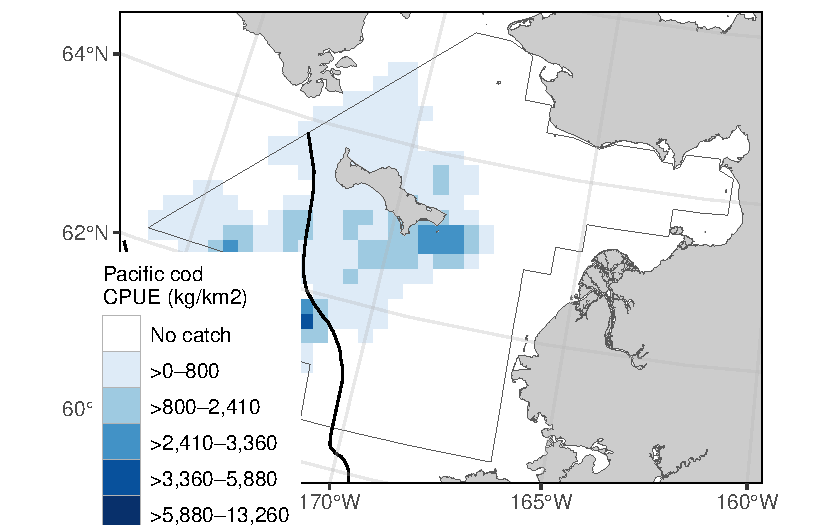
\includegraphics{content/foss-api-r_files/figure-pdf/test-7-fig-1.pdf}

}

\caption{Ex. 7: Visualize CPUE data in distribution map.}

\end{figure}

\hypertarget{access-via-api-and-python}{%
\chapter{Access via API and Python}\label{access-via-api-and-python}}

\hypertarget{afscgap-library-installation}{%
\subsection{\{afscgap\} Library
Installation}\label{afscgap-library-installation}}

\begin{quote}
author: Sam Pottinger (sam.pottinger@berkeley.edu; GitHub::sampottinger)
date: May 13, 2023
\end{quote}

The third-party \texttt{afscgap} Python package interfaces with FOSS to
access AFSC GAP data. It can be installed via pip:

\begin{Shaded}
\begin{Highlighting}[]
\CommentTok{\#The reticulate package provides a comprehensive set of tools for interoperability between Python and R. }
\FunctionTok{library}\NormalTok{(reticulate)}
\end{Highlighting}
\end{Shaded}

\begin{Shaded}
\begin{Highlighting}[]
\NormalTok{pip install afscgap}
\NormalTok{pip install git}\SpecialCharTok{+}\NormalTok{https}\SpecialCharTok{:}\ErrorTok{//}\NormalTok{github.com}\SpecialCharTok{/}\NormalTok{SchmidtDSE}\SpecialCharTok{/}\NormalTok{afscgap.git}\SpecialCharTok{@}\NormalTok{main}
\end{Highlighting}
\end{Shaded}

For more information on installation and deployment, see the
\href{https://pyafscgap.org}{library documentation}.

\hypertarget{basic-query}{%
\subsection{Basic query}\label{basic-query}}

This first example queries for Pacific glass shrimp (\emph{Pasiphaea
pacifica}) in the Gulf of Alaska in 2021. The library will automatically
generate HTTP queries, converting from Python types to
\href{https://www.oracle.com/database/technologies/appdev/rest.html}{ORDS}
query syntax.

\begin{Shaded}
\begin{Highlighting}[]
\NormalTok{import afscgap}

\NormalTok{query }\OtherTok{=} \FunctionTok{afscgap.Query}\NormalTok{()}
\FunctionTok{query.filter\_year}\NormalTok{(}\AttributeTok{eq=}\DecValTok{2021}\NormalTok{)}
\FunctionTok{query.filter\_srvy}\NormalTok{(}\AttributeTok{eq=}\StringTok{\textquotesingle{}GOA\textquotesingle{}}\NormalTok{)}
\FunctionTok{query.filter\_scientific\_name}\NormalTok{(}\AttributeTok{eq=}\StringTok{\textquotesingle{}Pasiphaea pacifica\textquotesingle{}}\NormalTok{)}

\NormalTok{results }\OtherTok{=} \FunctionTok{query.execute}\NormalTok{()}
\end{Highlighting}
\end{Shaded}

The \texttt{results} variable in this example is an iterator that will
automatically perform pagination behind the scenes.

\hypertarget{iterating-with-a-for-loop}{%
\subsection{Iterating with a for loop}\label{iterating-with-a-for-loop}}

The easiest way to interact with results is a simple for loop. This next
example determines the frequency of different catch per unit effort
where Pacific glass shrimp were reported:

\begin{Shaded}
\begin{Highlighting}[]
\NormalTok{import afscgap}

\CommentTok{\# Mapping from CPUE to count}
\NormalTok{count\_by\_cpue }\OtherTok{=}\NormalTok{ \{\}}

\CommentTok{\# Build query}
\NormalTok{query }\OtherTok{=} \FunctionTok{afscgap.Query}\NormalTok{()}
\FunctionTok{query.filter\_year}\NormalTok{(}\AttributeTok{eq=}\DecValTok{2021}\NormalTok{)}
\FunctionTok{query.filter\_srvy}\NormalTok{(}\AttributeTok{eq=}\StringTok{\textquotesingle{}GOA\textquotesingle{}}\NormalTok{)}
\FunctionTok{query.filter\_scientific\_name}\NormalTok{(}\AttributeTok{eq=}\StringTok{\textquotesingle{}Pasiphaea pacifica\textquotesingle{}}\NormalTok{)}
\NormalTok{results }\OtherTok{=} \FunctionTok{query.execute}\NormalTok{()}

\CommentTok{\# Iterate through results and count}
\ControlFlowTok{for}\NormalTok{ record }\ControlFlowTok{in}\NormalTok{ results}\SpecialCharTok{:}
\NormalTok{  cpue }\OtherTok{=} \FunctionTok{record.get\_cpue\_weight}\NormalTok{(}\AttributeTok{units=}\StringTok{\textquotesingle{}kg/ha\textquotesingle{}}\NormalTok{)}
\NormalTok{  cpue\_rounded }\OtherTok{=} \FunctionTok{round}\NormalTok{(cpue)}
\NormalTok{  count }\OtherTok{=} \FunctionTok{count\_by\_cpue.get}\NormalTok{(cpue\_rounded, }\DecValTok{0}\NormalTok{) }\SpecialCharTok{+} \DecValTok{1}
\NormalTok{  count\_by\_cpue[cpue\_rounded] }\OtherTok{=}\NormalTok{ count}

\CommentTok{\# Print the result}
\FunctionTok{print}\NormalTok{(count\_by\_cpue)}
\end{Highlighting}
\end{Shaded}

Note that, in this example, only records with Pacific glass shrimp are
included (``presence-only'' data). See zero catch inference below. In
other words, it reports on CPUE only for hauls in which Pacific glass
shrimp were recorded, excluding some hauls like those in which Pacific
glass shrimp were not found at all.

\hypertarget{iterating-with-functional-programming}{%
\subsection{Iterating with functional
programming}\label{iterating-with-functional-programming}}

A for loop is not the only option for iterating through results. List
comprehensions and other functional programming methods can be used as
well.

\begin{Shaded}
\begin{Highlighting}[]
\NormalTok{import statistics}

\NormalTok{import afscgap}

\CommentTok{\# Build query}
\NormalTok{query }\OtherTok{=} \FunctionTok{afscgap.Query}\NormalTok{()}
\FunctionTok{query.filter\_year}\NormalTok{(}\AttributeTok{eq=}\DecValTok{2021}\NormalTok{)}
\FunctionTok{query.filter\_srvy}\NormalTok{(}\AttributeTok{eq=}\StringTok{\textquotesingle{}GOA\textquotesingle{}}\NormalTok{)}
\FunctionTok{query.filter\_scientific\_name}\NormalTok{(}\AttributeTok{eq=}\StringTok{\textquotesingle{}Pasiphaea pacifica\textquotesingle{}}\NormalTok{)}
\NormalTok{results }\OtherTok{=} \FunctionTok{query.execute}\NormalTok{()}

\CommentTok{\# Get temperatures in Celsius}
\NormalTok{temperatures }\OtherTok{=}\NormalTok{ [}\FunctionTok{record.get\_bottom\_temperature}\NormalTok{(}\AttributeTok{units=}\StringTok{\textquotesingle{}c\textquotesingle{}}\NormalTok{) }\ControlFlowTok{for}\NormalTok{ record }\ControlFlowTok{in}\NormalTok{ results]}

\CommentTok{\# Take the median}
\FunctionTok{print}\NormalTok{(}\FunctionTok{statistics.median}\NormalTok{(temperatures))}
\end{Highlighting}
\end{Shaded}

This example reports the median temperature in Celcius for when Pacific
glass shrimp was reported.

\hypertarget{load-into-pandas}{%
\subsection{Load into Pandas}\label{load-into-pandas}}

The results from the \texttt{afscgap} package are serializable and can
be loaded into other tools like
\href{https://pandas.pydata.org/}{Pandas}. This example loads Pacific
glass shrimp from 2021 Gulf of Alaska into a data frame.

\begin{Shaded}
\begin{Highlighting}[]
\NormalTok{import pandas}

\NormalTok{import afscgap}

\NormalTok{query }\OtherTok{=} \FunctionTok{afscgap.Query}\NormalTok{()}
\FunctionTok{query.filter\_year}\NormalTok{(}\AttributeTok{eq=}\DecValTok{2021}\NormalTok{)}
\FunctionTok{query.filter\_srvy}\NormalTok{(}\AttributeTok{eq=}\StringTok{\textquotesingle{}GOA\textquotesingle{}}\NormalTok{)}
\FunctionTok{query.filter\_scientific\_name}\NormalTok{(}\AttributeTok{eq=}\StringTok{\textquotesingle{}Pasiphaea pacifica\textquotesingle{}}\NormalTok{)}
\NormalTok{results }\OtherTok{=} \FunctionTok{query.execute}\NormalTok{()}

\FunctionTok{pandas.DataFrame}\NormalTok{(}\FunctionTok{results.to\_dicts}\NormalTok{())}
\end{Highlighting}
\end{Shaded}

Specifically, \texttt{to\_dicts} provides an iterator over a dictionary
form of the data that can be read into tools like Pandas.

\hypertarget{advanced-filtering}{%
\subsection{Advanced filtering}\label{advanced-filtering}}

Queries so far have focused on filters requiring equality but range
queries can be built as well.

\begin{Shaded}
\begin{Highlighting}[]
\NormalTok{import afscgap}

\CommentTok{\# Build query}
\NormalTok{query }\OtherTok{=} \FunctionTok{afscgap.Query}\NormalTok{()}
\FunctionTok{query.filter\_year}\NormalTok{(}\AttributeTok{min\_val=}\DecValTok{2015}\NormalTok{, }\AttributeTok{max\_val=}\DecValTok{2019}\NormalTok{)   }\CommentTok{\# Note min/max\_val}
\FunctionTok{query.filter\_srvy}\NormalTok{(}\AttributeTok{eq=}\StringTok{\textquotesingle{}GOA\textquotesingle{}}\NormalTok{)}
\FunctionTok{query.filter\_scientific\_name}\NormalTok{(}\AttributeTok{eq=}\StringTok{\textquotesingle{}Pasiphaea pacifica\textquotesingle{}}\NormalTok{)}
\NormalTok{results }\OtherTok{=} \FunctionTok{query.execute}\NormalTok{()}

\CommentTok{\# Sum weight}
\NormalTok{weights }\OtherTok{=} \FunctionTok{map}\NormalTok{(lambda x}\SpecialCharTok{:} \FunctionTok{x.get\_weight}\NormalTok{(}\AttributeTok{units=}\StringTok{\textquotesingle{}kg\textquotesingle{}}\NormalTok{), results)}
\NormalTok{total\_weight }\OtherTok{=} \FunctionTok{sum}\NormalTok{(weights)}
\FunctionTok{print}\NormalTok{(total\_weight)}
\end{Highlighting}
\end{Shaded}

This example queries for Pacific glass shrimp data between 2015 and
2019, summing the total weight caught. Note that most users will likely
take advantage of built-in Python to
\href{https://www.oracle.com/database/technologies/appdev/rest.html}{ORDS}
query generation which dictates how the library communicates with the
API service. However, users can provide raw ORDS queries as well using
\href{https://pyafscgap.org/devdocs/afscgap.html\#manual-filtering}{manual
filtering}.

\hypertarget{zero-catch-inference}{%
\subsection{Zero-catch inference}\label{zero-catch-inference}}

Until this point, these examples use presence-only data. However, the
\texttt{afscgap} package can infer negative or ``zero catch'' records as
well.

\begin{Shaded}
\begin{Highlighting}[]
\NormalTok{import afscgap}

\CommentTok{\# Mapping from CPUE to count}
\NormalTok{count\_by\_cpue }\OtherTok{=}\NormalTok{ \{\}}

\CommentTok{\# Build query}
\NormalTok{query }\OtherTok{=} \FunctionTok{afscgap.Query}\NormalTok{()}
\FunctionTok{query.filter\_year}\NormalTok{(}\AttributeTok{eq=}\DecValTok{2021}\NormalTok{)}
\FunctionTok{query.filter\_srvy}\NormalTok{(}\AttributeTok{eq=}\StringTok{\textquotesingle{}GOA\textquotesingle{}}\NormalTok{)}
\FunctionTok{query.filter\_scientific\_name}\NormalTok{(}\AttributeTok{eq=}\StringTok{\textquotesingle{}Pasiphaea pacifica\textquotesingle{}}\NormalTok{)}
\FunctionTok{query.set\_presence\_only}\NormalTok{(False)  }\CommentTok{\# Added to earlier example}
\NormalTok{results }\OtherTok{=} \FunctionTok{query.execute}\NormalTok{()}

\CommentTok{\# Iterate through results and count}
\ControlFlowTok{for}\NormalTok{ record }\ControlFlowTok{in}\NormalTok{ results}\SpecialCharTok{:}
\NormalTok{  cpue }\OtherTok{=} \FunctionTok{record.get\_cpue\_weight}\NormalTok{(}\AttributeTok{units=}\StringTok{\textquotesingle{}kg/ha\textquotesingle{}}\NormalTok{)}
\NormalTok{  cpue\_rounded }\OtherTok{=} \FunctionTok{round}\NormalTok{(cpue)}
\NormalTok{  count }\OtherTok{=} \FunctionTok{count\_by\_cpue.get}\NormalTok{(cpue\_rounded, }\DecValTok{0}\NormalTok{) }\SpecialCharTok{+} \DecValTok{1}
\NormalTok{  count\_by\_cpue[cpue\_rounded] }\OtherTok{=}\NormalTok{ count}

\CommentTok{\# Print the result}
\FunctionTok{print}\NormalTok{(count\_by\_cpue)}
\end{Highlighting}
\end{Shaded}

This example revisits the earlier snippet for CPUE counts but
\texttt{set\_presence\_only(False)} directs the library to look at
additional data on hauls, determining which hauls did not have Pacific
glass shrimp. This lets the library return records for hauls in which
Pacific glass shrimp were not found. This can be seen in differences in
counts reported:

\begin{longtable}[]{@{}
  >{\raggedright\arraybackslash}p{(\columnwidth - 4\tabcolsep) * \real{0.1609}}
  >{\raggedright\arraybackslash}p{(\columnwidth - 4\tabcolsep) * \real{0.4138}}
  >{\raggedright\arraybackslash}p{(\columnwidth - 4\tabcolsep) * \real{0.4253}}@{}}
\toprule\noalign{}
\begin{minipage}[b]{\linewidth}\raggedright
Rounded CPUE
\end{minipage} & \begin{minipage}[b]{\linewidth}\raggedright
Count with set\_presence\_only(True)
\end{minipage} & \begin{minipage}[b]{\linewidth}\raggedright
Count with set\_presence\_only(False)
\end{minipage} \\
\midrule\noalign{}
\endhead
\bottomrule\noalign{}
\endlastfoot
0 kg/ha & 44 & 521 \\
1 kg/ha & 7 & 7 \\
2 kg/ha & 1 & 1 \\
\end{longtable}

Put simply, while the earlier example showed CPUE counts for hauls in
which Pacific glass shrimp were seen, this revised example reports for
all hauls in the Gulf of Alaska in 2021.

\hypertarget{more-information}{%
\subsection{More information}\label{more-information}}

Please see the \href{https://pyafscgap.org/devdocs/afscgap.html}{API
documentation} for the Python library for additional details.

\hypertarget{access-via-oracle-and-r-afsc-only}{%
\chapter{Access via Oracle and R (AFSC
only)}\label{access-via-oracle-and-r-afsc-only}}

If the user has access to the AFSC \texttt{Oracle} database, the user
can use \texttt{SQL\ developer} to view and pull the FOSS public data
directly from the \texttt{GAP\_PRODUCTS} \texttt{Oracle} schema.

\hypertarget{connect-to-oracle-from-r-1}{%
\subsection{Connect to Oracle from R}\label{connect-to-oracle-from-r-1}}

Many users will want to access the data from \texttt{Oracle} using
\texttt{R}. The user will need to install the \texttt{RODBC} \texttt{R}
package and ask OFIS (IT) connect \texttt{R} to \texttt{Oracle}. Then,
use the following code in \texttt{R} to establish a connection from
\texttt{R} to \texttt{Oracle}:

Here, the user can write in their username and password directly into
the \texttt{RODBC} connect function. Never save usernames or passwords
in scripts that may be intentionally or unintentionally shared with
others. If no username and password is entered in the function, pop-ups
will appear on the screen asking for the username and password.

\begin{Shaded}
\begin{Highlighting}[]
\FunctionTok{library}\NormalTok{(gapindex)}
\NormalTok{channel }\OtherTok{\textless{}{-}}\NormalTok{ gapindex}\SpecialCharTok{::}\FunctionTok{get\_connected}\NormalTok{()}
\end{Highlighting}
\end{Shaded}

\hypertarget{ex.-1-join-data}{%
\subsection{Ex. 1: Join data}\label{ex.-1-join-data}}

To join these tables in Oracle, you may use a variant of the following
code:

\begin{Shaded}
\begin{Highlighting}[]
\KeywordTok{SELECT} 
\NormalTok{hh.}\DataTypeTok{YEAR}\NormalTok{,}
\NormalTok{hh.SRVY,                 }
\NormalTok{hh.SURVEY,}
\NormalTok{hh.SURVEY\_DEFINITION\_ID,}
\NormalTok{hh.SURVEY\_NAME,}
\NormalTok{hh.CRUISE,}
\NormalTok{hh.CRUISEJOIN,           }
\NormalTok{hh.HAUL,}
\NormalTok{hh.HAULJOIN,}
\NormalTok{hh.STRATUM,}
\NormalTok{hh.STATION,}
\NormalTok{hh.VESSEL\_ID,}
\NormalTok{hh.VESSEL\_NAME,          }
\NormalTok{hh.DATE\_TIME,}
\NormalTok{hh.LATITUDE\_DD\_START, }
\NormalTok{hh.LONGITUDE\_DD\_START, }
\NormalTok{hh.LATITUDE\_DD\_END,}
\NormalTok{hh.LONGITUDE\_DD\_END, }
\NormalTok{hh.BOTTOM\_TEMPERATURE\_C,}
\NormalTok{hh.SURFACE\_TEMPERATURE\_C,}
\NormalTok{hh.DEPTH\_M,}
\NormalTok{cc.SPECIES\_CODE,}
\NormalTok{ss.ITIS,}
\NormalTok{ss.WORMS,}
\NormalTok{ss.COMMON\_NAME,     }
\NormalTok{ss.SCIENTIFIC\_NAME,}
\NormalTok{ss.ID\_RANK,}
\ControlFlowTok{CASE} \ControlFlowTok{WHEN}\NormalTok{ cc.CPUE\_KGKM2 }\KeywordTok{IS} \KeywordTok{NULL} \ControlFlowTok{THEN} \DecValTok{0} \ControlFlowTok{ELSE}\NormalTok{ cc.CPUE\_KGKM2 }\ControlFlowTok{END} \KeywordTok{AS}\NormalTok{ CPUE\_KGKM2,}
\ControlFlowTok{CASE} \ControlFlowTok{WHEN}\NormalTok{ cc.CPUE\_NOKM2 }\KeywordTok{IS} \KeywordTok{NULL} \ControlFlowTok{THEN} \DecValTok{0} \ControlFlowTok{ELSE}\NormalTok{ cc.CPUE\_NOKM2 }\ControlFlowTok{END} \KeywordTok{AS}\NormalTok{ CPUE\_NOKM2,}
\ControlFlowTok{CASE} \ControlFlowTok{WHEN}\NormalTok{ cc.}\FunctionTok{COUNT} \KeywordTok{IS} \KeywordTok{NULL} \ControlFlowTok{THEN} \DecValTok{0} \ControlFlowTok{ELSE}\NormalTok{ cc.}\FunctionTok{COUNT} \ControlFlowTok{END} \KeywordTok{AS} \FunctionTok{COUNT}\NormalTok{,}
\ControlFlowTok{CASE} \ControlFlowTok{WHEN}\NormalTok{ cc.WEIGHT\_KG }\KeywordTok{IS} \KeywordTok{NULL} \ControlFlowTok{THEN} \DecValTok{0} \ControlFlowTok{ELSE}\NormalTok{ cc.WEIGHT\_KG }\ControlFlowTok{END} \KeywordTok{AS}\NormalTok{ WEIGHT\_KG,}
\ControlFlowTok{CASE} \ControlFlowTok{WHEN}\NormalTok{ cc.TAXON\_CONFIDENCE }\KeywordTok{IS} \KeywordTok{NULL} \ControlFlowTok{THEN} \KeywordTok{NULL} \ControlFlowTok{ELSE}\NormalTok{ cc.TAXON\_CONFIDENCE }\ControlFlowTok{END} \KeywordTok{AS}\NormalTok{ TAXON\_CONFIDENCE,}
\NormalTok{hh.AREA\_SWEPT\_KM2,       }
\NormalTok{hh.DISTANCE\_FISHED\_KM,}
\NormalTok{hh.DURATION\_HR,          }
\NormalTok{hh.NET\_WIDTH\_M,}
\NormalTok{hh.NET\_HEIGHT\_M,}
\NormalTok{hh.PERFORMANCE }
\KeywordTok{FROM}\NormalTok{ GAP\_PRODUCTS.FOSS\_SURVEY\_SPECIES sv}
\KeywordTok{FULL} \KeywordTok{OUTER} \KeywordTok{JOIN}\NormalTok{ GAP\_PRODUCTS.FOSS\_SPECIES ss}
\KeywordTok{ON}\NormalTok{ sv.SPECIES\_CODE }\OperatorTok{=}\NormalTok{ ss.SPECIES\_CODE}
\KeywordTok{FULL} \KeywordTok{OUTER} \KeywordTok{JOIN}\NormalTok{ GAP\_PRODUCTS.FOSS\_HAUL hh}
\KeywordTok{ON}\NormalTok{ sv.SURVEY\_DEFINITION\_ID }\OperatorTok{=}\NormalTok{ hh.SURVEY\_DEFINITION\_ID}
\KeywordTok{FULL} \KeywordTok{OUTER} \KeywordTok{JOIN}\NormalTok{ GAP\_PRODUCTS.FOSS\_CATCH cc}
\KeywordTok{ON}\NormalTok{ sv.SPECIES\_CODE }\OperatorTok{=}\NormalTok{ cc.SPECIES\_CODE}
\KeywordTok{AND}\NormalTok{ hh.HAULJOIN }\OperatorTok{=}\NormalTok{ cc.HAULJOIN}
\end{Highlighting}
\end{Shaded}

\hypertarget{ex.-2-subset-data}{%
\subsection{Ex. 2: Subset data}\label{ex.-2-subset-data}}

Once connected, pull and save (if needed) the tables into the \texttt{R}
environment.

To pull a small subset of the data (especially since files like
\texttt{GAP\_PRODUCTS.FOSS\_CPUE\_ZEROFILLED} are so big), use a
variation of the following code. Here, we are pulling EBS Pacific cod
from 2010 - 2021:

\begin{Shaded}
\begin{Highlighting}[]
\CommentTok{\# Pull data}
\NormalTok{a }\OtherTok{\textless{}{-}}\NormalTok{ RODBC}\SpecialCharTok{::}\FunctionTok{sqlQuery}\NormalTok{(}
\AttributeTok{channel =}\NormalTok{ channel, }
\AttributeTok{query =} 
\StringTok{"SELECT * FROM GAP\_PRODUCTS.FOSS\_CATCH cc}
\StringTok{JOIN GAP\_PRODUCTS.FOSS\_HAUL hh}
\StringTok{ON cc.HAULJOIN = hh.HAULJOIN}
\StringTok{WHERE SRVY = \textquotesingle{}EBS\textquotesingle{} }
\StringTok{AND SPECIES\_CODE = 21720 {-}{-} \textquotesingle{}Pacific cod\textquotesingle{} }
\StringTok{AND YEAR \textgreater{}= 2010 }
\StringTok{AND YEAR \textless{} 2021"}\NormalTok{)}
\CommentTok{\# Save table to local directory}
\FunctionTok{write.csv}\NormalTok{(}\AttributeTok{x =}\NormalTok{ a, }\AttributeTok{file =} \StringTok{"ebs\_pcod\_2010{-}2020.csv"}\NormalTok{)}
\end{Highlighting}
\end{Shaded}

\part{Product Outputs}

To accompany these data, we also produce data products to make using our
data more accessible and straightforward.

\global\setlength{\Oldarrayrulewidth}{\arrayrulewidth}

\global\setlength{\Oldtabcolsep}{\tabcolsep}

\setlength{\tabcolsep}{0pt}

\renewcommand*{\arraystretch}{1.5}



\providecommand{\ascline}[3]{\noalign{\global\arrayrulewidth #1}\arrayrulecolor[HTML]{#2}\cline{#3}}

\begin{longtable}[c]{|p{2.00in}|p{1.50in}|p{1.50in}|p{3.00in}}
\caption{Survey of products developed by GAP}\tabularnewline




\hhline{>{\arrayrulecolor[HTML]{000000}\global\arrayrulewidth=0pt}->{\arrayrulecolor[HTML]{000000}\global\arrayrulewidth=0pt}->{\arrayrulecolor[HTML]{000000}\global\arrayrulewidth=0pt}->{\arrayrulecolor[HTML]{000000}\global\arrayrulewidth=0pt}-}

\multicolumn{1}{>{\cellcolor[HTML]{CFCFCF}\raggedright}m{\dimexpr 2in+0\tabcolsep}}{\textcolor[HTML]{000000}{\fontsize{10}{10}\selectfont{\textbf{Product}}}} & \multicolumn{1}{>{\cellcolor[HTML]{CFCFCF}\raggedright}m{\dimexpr 1.5in+0\tabcolsep}}{\textcolor[HTML]{000000}{\fontsize{10}{10}\selectfont{\textbf{Point\ of\ Contact}}}\textcolor[HTML]{000000}{\fontsize{10}{10}\selectfont{\textbf{\linebreak }}}\textcolor[HTML]{000000}{\fontsize{10}{10}\selectfont{\textbf{GOA/AI}}}} & \multicolumn{1}{>{\cellcolor[HTML]{CFCFCF}\raggedright}m{\dimexpr 1.5in+0\tabcolsep}}{\textcolor[HTML]{000000}{\fontsize{10}{10}\selectfont{\textbf{Point\ of\ Contact}}}\textcolor[HTML]{000000}{\fontsize{10}{10}\selectfont{\textbf{\linebreak }}}\textcolor[HTML]{000000}{\fontsize{10}{10}\selectfont{\textbf{BS}}}} & \multicolumn{1}{>{\cellcolor[HTML]{CFCFCF}\raggedright}m{\dimexpr 3in+0\tabcolsep}}{\textcolor[HTML]{000000}{\fontsize{10}{10}\selectfont{\textbf{Description}}}} \\

\noalign{\global\arrayrulewidth 0pt}\arrayrulecolor[HTML]{000000}

\endfirsthead 

\hhline{>{\arrayrulecolor[HTML]{000000}\global\arrayrulewidth=0pt}->{\arrayrulecolor[HTML]{000000}\global\arrayrulewidth=0pt}->{\arrayrulecolor[HTML]{000000}\global\arrayrulewidth=0pt}->{\arrayrulecolor[HTML]{000000}\global\arrayrulewidth=0pt}-}

\multicolumn{1}{>{\cellcolor[HTML]{CFCFCF}\raggedright}m{\dimexpr 2in+0\tabcolsep}}{\textcolor[HTML]{000000}{\fontsize{10}{10}\selectfont{\textbf{Product}}}} & \multicolumn{1}{>{\cellcolor[HTML]{CFCFCF}\raggedright}m{\dimexpr 1.5in+0\tabcolsep}}{\textcolor[HTML]{000000}{\fontsize{10}{10}\selectfont{\textbf{Point\ of\ Contact}}}\textcolor[HTML]{000000}{\fontsize{10}{10}\selectfont{\textbf{\linebreak }}}\textcolor[HTML]{000000}{\fontsize{10}{10}\selectfont{\textbf{GOA/AI}}}} & \multicolumn{1}{>{\cellcolor[HTML]{CFCFCF}\raggedright}m{\dimexpr 1.5in+0\tabcolsep}}{\textcolor[HTML]{000000}{\fontsize{10}{10}\selectfont{\textbf{Point\ of\ Contact}}}\textcolor[HTML]{000000}{\fontsize{10}{10}\selectfont{\textbf{\linebreak }}}\textcolor[HTML]{000000}{\fontsize{10}{10}\selectfont{\textbf{BS}}}} & \multicolumn{1}{>{\cellcolor[HTML]{CFCFCF}\raggedright}m{\dimexpr 3in+0\tabcolsep}}{\textcolor[HTML]{000000}{\fontsize{10}{10}\selectfont{\textbf{Description}}}} \\

\noalign{\global\arrayrulewidth 0pt}\arrayrulecolor[HTML]{000000}

\endhead



\multicolumn{4}{>{\cellcolor[HTML]{B3B3B3}\raggedright}m{\dimexpr 8in+6\tabcolsep}}{\textcolor[HTML]{000000}{\fontsize{10}{10}\selectfont{\textit{Data}}}} \\

\noalign{\global\arrayrulewidth 0pt}\arrayrulecolor[HTML]{000000}





\multicolumn{1}{>{\raggedright}m{\dimexpr 2in+0\tabcolsep}}{\textcolor[HTML]{00008B}{\fontsize{10}{10}\selectfont{\textbf{\href{https://github.com/afsc-gap-products/data-requests}{Finalized\ bottom\ trawl\ data}}}}} & \multicolumn{1}{>{\raggedright}m{\dimexpr 1.5in+0\tabcolsep}}{\textcolor[HTML]{000000}{\fontsize{10}{10}\selectfont{Ned\ Laman}}} & \multicolumn{1}{>{\raggedright}m{\dimexpr 1.5in+0\tabcolsep}}{\textcolor[HTML]{000000}{\fontsize{10}{10}\selectfont{Duane\ Stevenson}}} & \multicolumn{1}{>{\raggedright}m{\dimexpr 3in+0\tabcolsep}}{\textcolor[HTML]{000000}{\fontsize{10}{10}\selectfont{NOAA-NMFS-AFSC-RACE-GAP\ bottom\ trawl\ data\ that\ has\ completed\ the\ post-survey\ internal\ QAQC\ process.}}} \\

\noalign{\global\arrayrulewidth 0pt}\arrayrulecolor[HTML]{000000}





\multicolumn{1}{>{\cellcolor[HTML]{EFEFEF}\raggedright}m{\dimexpr 2in+0\tabcolsep}}{\textcolor[HTML]{00008B}{\fontsize{10}{10}\selectfont{\textbf{\href{https://github.com/afsc-gap-products/data-requests}{Data\ requests}}}}} & \multicolumn{1}{>{\cellcolor[HTML]{EFEFEF}\raggedright}m{\dimexpr 1.5in+0\tabcolsep}}{\textcolor[HTML]{000000}{\fontsize{10}{10}\selectfont{Nancy\ Roberson}}} & \multicolumn{1}{>{\cellcolor[HTML]{EFEFEF}\raggedright}m{\dimexpr 1.5in+0\tabcolsep}}{\textcolor[HTML]{000000}{\fontsize{10}{10}\selectfont{Nancy\ Roberson}}} & \multicolumn{1}{>{\cellcolor[HTML]{EFEFEF}\raggedright}m{\dimexpr 3in+0\tabcolsep}}{\textcolor[HTML]{000000}{\fontsize{10}{10}\selectfont{To\ request\ a\ subset\ of\ the\ NOAA-NMFS-AFSC-RACE-GAP\ bottom\ trawl\ raw\ data\ or\ a\ data\ product.}}} \\

\noalign{\global\arrayrulewidth 0pt}\arrayrulecolor[HTML]{000000}





\multicolumn{1}{>{\raggedright}m{\dimexpr 2in+0\tabcolsep}}{\textcolor[HTML]{00008B}{\fontsize{10}{10}\selectfont{\textbf{\href{https://www.fisheries.noaa.gov/resource/document/groundfish-survey-species-code-manual-and-data-codes-manual}{Species\ codebook}}}}} & \multicolumn{1}{>{\raggedright}m{\dimexpr 1.5in+0\tabcolsep}}{\textcolor[HTML]{000000}{\fontsize{10}{10}\selectfont{Nancy\ Roberson}}} & \multicolumn{1}{>{\raggedright}m{\dimexpr 1.5in+0\tabcolsep}}{\textcolor[HTML]{000000}{\fontsize{10}{10}\selectfont{Chris\ Anderson}}} & \multicolumn{1}{>{\raggedright}m{\dimexpr 3in+0\tabcolsep}}{\textcolor[HTML]{000000}{\fontsize{10}{10}\selectfont{List\ of\ codes\ used\ for\ fish\ and\ invertebrates\ identified\ in\ NOAA-NMFS-AFSC-RACE-GAP\ Division\ surveys.\ }}} \\

\noalign{\global\arrayrulewidth 0pt}\arrayrulecolor[HTML]{000000}





\multicolumn{1}{>{\cellcolor[HTML]{EFEFEF}\raggedright}m{\dimexpr 2in+0\tabcolsep}}{\textcolor[HTML]{00008B}{\fontsize{10}{10}\selectfont{\textbf{\href{https://repository.library.noaa.gov/view/noaa/12855}{Survey\ protocols}}}}} & \multicolumn{1}{>{\cellcolor[HTML]{EFEFEF}\raggedright}m{\dimexpr 1.5in+0\tabcolsep}}{\textcolor[HTML]{000000}{\fontsize{10}{10}\selectfont{Nancy\ Roberson}}} & \multicolumn{1}{>{\cellcolor[HTML]{EFEFEF}\raggedright}m{\dimexpr 1.5in+0\tabcolsep}}{\textcolor[HTML]{000000}{\fontsize{10}{10}\selectfont{Nancy\ Roberson}}} & \multicolumn{1}{>{\cellcolor[HTML]{EFEFEF}\raggedright}m{\dimexpr 3in+0\tabcolsep}}{\textcolor[HTML]{000000}{\fontsize{10}{10}\selectfont{Documentation\ of\ NOAA-NMFS-AFSC-RACE-GAP\ groundfish\ bottom\ trawl\ survey\ protocols.}}} \\

\noalign{\global\arrayrulewidth 0pt}\arrayrulecolor[HTML]{000000}





\multicolumn{4}{>{\cellcolor[HTML]{B3B3B3}\raggedright}m{\dimexpr 8in+6\tabcolsep}}{\textcolor[HTML]{000000}{\fontsize{10}{10}\selectfont{\textit{Analysis}}}} \\

\noalign{\global\arrayrulewidth 0pt}\arrayrulecolor[HTML]{000000}





\multicolumn{1}{>{\cellcolor[HTML]{EFEFEF}\raggedright}m{\dimexpr 2in+0\tabcolsep}}{\textcolor[HTML]{00008B}{\fontsize{10}{10}\selectfont{\textbf{\href{https://github.com/afsc-gap-products/gapindex}{Design-based\ indices\ for\ target\ species}}}}} & \multicolumn{1}{>{\cellcolor[HTML]{EFEFEF}\raggedright}m{\dimexpr 1.5in+0\tabcolsep}}{\textcolor[HTML]{000000}{\fontsize{10}{10}\selectfont{Ned\ Laman}}} & \multicolumn{1}{>{\cellcolor[HTML]{EFEFEF}\raggedright}m{\dimexpr 1.5in+0\tabcolsep}}{\textcolor[HTML]{000000}{\fontsize{10}{10}\selectfont{Rebecca\ Haehn}}} & \multicolumn{1}{>{\cellcolor[HTML]{EFEFEF}\raggedright}m{\dimexpr 3in+0\tabcolsep}}{\textcolor[HTML]{000000}{\fontsize{10}{10}\selectfont{Standard\ design-based\ indices\ of\ biomass\ and\ abundance\ from\ NOAA-NMFS-AFSC-RACE-GAP\ bottom\ trawl\ survey\ data.}}} \\

\noalign{\global\arrayrulewidth 0pt}\arrayrulecolor[HTML]{000000}





\multicolumn{1}{>{\raggedright}m{\dimexpr 2in+0\tabcolsep}}{\textcolor[HTML]{00008B}{\fontsize{10}{10}\selectfont{\textbf{\href{https://github.com/afsc-gap-products/gapindex}{Design-based\ age\ or\ length\ composition}}}}} & \multicolumn{1}{>{\raggedright}m{\dimexpr 1.5in+0\tabcolsep}}{\textcolor[HTML]{000000}{\fontsize{10}{10}\selectfont{Ned\ Laman}}} & \multicolumn{1}{>{\raggedright}m{\dimexpr 1.5in+0\tabcolsep}}{\textcolor[HTML]{000000}{\fontsize{10}{10}\selectfont{Rebecca\ Haehn}}} & \multicolumn{1}{>{\raggedright}m{\dimexpr 3in+0\tabcolsep}}{\textcolor[HTML]{000000}{\fontsize{10}{10}\selectfont{Standard\ design-based\ indices\ of\ size\ and\ age\ composition\ from\ NOAA-NMFS-AFSC-RACE-GAP\ bottom\ trawl\ survey\ data.}}} \\

\noalign{\global\arrayrulewidth 0pt}\arrayrulecolor[HTML]{000000}





\multicolumn{1}{>{\cellcolor[HTML]{EFEFEF}\raggedright}m{\dimexpr 2in+0\tabcolsep}}{\textcolor[HTML]{00008B}{\fontsize{10}{10}\selectfont{\textbf{\href{https://github.com/afsc-gap-products/model-based-indices}{Model-based\ indices,\ age\ comps\ (stock\ assessment),\ area\ occupied,\ and\ COG\ (ESP)}}}}} & \multicolumn{1}{>{\cellcolor[HTML]{EFEFEF}\raggedright}m{\dimexpr 1.5in+0\tabcolsep}}{\textcolor[HTML]{000000}{\fontsize{10}{10}\selectfont{Cecilia\ O'Leary\ }}} & \multicolumn{1}{>{\cellcolor[HTML]{EFEFEF}\raggedright}m{\dimexpr 1.5in+0\tabcolsep}}{\textcolor[HTML]{000000}{\fontsize{10}{10}\selectfont{Lewis\ Barnett}}} & \multicolumn{1}{>{\cellcolor[HTML]{EFEFEF}\raggedright}m{\dimexpr 3in+0\tabcolsep}}{\textcolor[HTML]{000000}{\fontsize{10}{10}\selectfont{Spatiotemporal\ model-based\ biomass\ indices,\ abundance\ indices,\ and\ age\ composition\ from\ NOAA-NMFS-AFSC-RACE-GAP\ bottom\ trawl\ survey\ data.}}} \\

\noalign{\global\arrayrulewidth 0pt}\arrayrulecolor[HTML]{000000}





\multicolumn{1}{>{\raggedright}m{\dimexpr 2in+0\tabcolsep}}{\textcolor[HTML]{00008B}{\fontsize{10}{10}\selectfont{\textbf{\href{}{Annual\ bottom\ and\ surface\ temperature\ summary\ (ESR,\ stock\ assessment)}}}}} & \multicolumn{1}{>{\raggedright}m{\dimexpr 1.5in+0\tabcolsep}}{\textcolor[HTML]{000000}{\fontsize{10}{10}\selectfont{Cecilia\ O'Leary}}} & \multicolumn{1}{>{\raggedright}m{\dimexpr 1.5in+0\tabcolsep}}{\textcolor[HTML]{000000}{\fontsize{10}{10}\selectfont{Sean\ Rohan\ \&}}\textcolor[HTML]{000000}{\fontsize{10}{10}\selectfont{\linebreak }}\textcolor[HTML]{000000}{\fontsize{10}{10}\selectfont{Lewis\ Barnett}}} & \multicolumn{1}{>{\raggedright}m{\dimexpr 3in+0\tabcolsep}}{\textcolor[HTML]{000000}{\fontsize{10}{10}\selectfont{Summary\ metrics\ for\ bottom\ trawl\ bottom\ and\ surface\ temperatures\ relative\ to\ historical\ baseline.}}} \\

\noalign{\global\arrayrulewidth 0pt}\arrayrulecolor[HTML]{000000}





\multicolumn{1}{>{\cellcolor[HTML]{EFEFEF}\raggedright}m{\dimexpr 2in+0\tabcolsep}}{\textcolor[HTML]{00008B}{\fontsize{10}{10}\selectfont{\textbf{\href{https://github.com/afsc-gap-products/gapctd}{Salinity\ indicator\ (ESR\ in\ 2024)}}}}} & \multicolumn{1}{>{\cellcolor[HTML]{EFEFEF}\raggedright}m{\dimexpr 1.5in+0\tabcolsep}}{\textcolor[HTML]{000000}{\fontsize{10}{10}\selectfont{-}}} & \multicolumn{1}{>{\cellcolor[HTML]{EFEFEF}\raggedright}m{\dimexpr 1.5in+0\tabcolsep}}{\textcolor[HTML]{000000}{\fontsize{10}{10}\selectfont{Sean\ Rohan\ \&}}\textcolor[HTML]{000000}{\fontsize{10}{10}\selectfont{\linebreak }}\textcolor[HTML]{000000}{\fontsize{10}{10}\selectfont{Ned\ Cokelet}}} & \multicolumn{1}{>{\cellcolor[HTML]{EFEFEF}\raggedright}m{\dimexpr 3in+0\tabcolsep}}{\textcolor[HTML]{000000}{\fontsize{10}{10}\selectfont{Developing\ salinity\ indicators\ (available\ in\ 2024).}}} \\

\noalign{\global\arrayrulewidth 0pt}\arrayrulecolor[HTML]{000000}





\multicolumn{1}{>{\raggedright}m{\dimexpr 2in+0\tabcolsep}}{\textcolor[HTML]{00008B}{\fontsize{10}{10}\selectfont{\textbf{\href{https://github.com/afsc-gap-products/coldpool}{Bering\ Sea\ cold\ pool\ index\ and\ temperature\ data\ products\ (ESR,\ ESP,\ stock\ assessment)}}}}} & \multicolumn{1}{>{\raggedright}m{\dimexpr 1.5in+0\tabcolsep}}{\textcolor[HTML]{000000}{\fontsize{10}{10}\selectfont{-}}} & \multicolumn{1}{>{\raggedright}m{\dimexpr 1.5in+0\tabcolsep}}{\textcolor[HTML]{000000}{\fontsize{10}{10}\selectfont{Sean\ Rohan\ \&}}\textcolor[HTML]{000000}{\fontsize{10}{10}\selectfont{\linebreak }}\textcolor[HTML]{000000}{\fontsize{10}{10}\selectfont{Lewis\ Barnett}}} & \multicolumn{1}{>{\raggedright}m{\dimexpr 3in+0\tabcolsep}}{\textcolor[HTML]{000000}{\fontsize{10}{10}\selectfont{Create\ annual\ temperature\ rasters\ for\ the\ EBS,\ calculate\ the\ EBS\ cold\ pool\ index\ and\ temperature\ data\ products,\ and\ produce\ visualizations.}}} \\

\noalign{\global\arrayrulewidth 0pt}\arrayrulecolor[HTML]{000000}





\multicolumn{1}{>{\cellcolor[HTML]{EFEFEF}\raggedright}m{\dimexpr 2in+0\tabcolsep}}{\textcolor[HTML]{00008B}{\fontsize{10}{10}\selectfont{\textbf{\href{https://github.com/afsc-gap-products/akfishcondition}{Annual\ fish\ condition\ (ESR)}}}}} & \multicolumn{1}{>{\cellcolor[HTML]{EFEFEF}\raggedright}m{\dimexpr 1.5in+0\tabcolsep}}{\textcolor[HTML]{000000}{\fontsize{10}{10}\selectfont{Cecilia\ O'Leary}}} & \multicolumn{1}{>{\cellcolor[HTML]{EFEFEF}\raggedright}m{\dimexpr 1.5in+0\tabcolsep}}{\textcolor[HTML]{000000}{\fontsize{10}{10}\selectfont{Bianca\ Prohaska\ \&}}\textcolor[HTML]{000000}{\fontsize{10}{10}\selectfont{\linebreak }}\textcolor[HTML]{000000}{\fontsize{10}{10}\selectfont{Sean\ Rohan}}} & \multicolumn{1}{>{\cellcolor[HTML]{EFEFEF}\raggedright}m{\dimexpr 3in+0\tabcolsep}}{\textcolor[HTML]{000000}{\fontsize{10}{10}\selectfont{Groundfish\ morphometric\ condition\ for\ fish\ in\ the\ Bering\ Sea,\ Aleutian\ Islands,\ and\ Gulf\ of\ Alaska.}}} \\

\noalign{\global\arrayrulewidth 0pt}\arrayrulecolor[HTML]{000000}





\multicolumn{1}{>{\raggedright}m{\dimexpr 2in+0\tabcolsep}}{\textcolor[HTML]{00008B}{\fontsize{10}{10}\selectfont{\textbf{\href{}{Rockfish\ indices\ vs\ environmental\ gradients\ (ESR)}}}}} & \multicolumn{1}{>{\raggedright}m{\dimexpr 1.5in+0\tabcolsep}}{\textcolor[HTML]{000000}{\fontsize{10}{10}\selectfont{Alexandra\ Dowlin}}} & \multicolumn{1}{>{\raggedright}m{\dimexpr 1.5in+0\tabcolsep}}{\textcolor[HTML]{000000}{\fontsize{10}{10}\selectfont{-}}} & \multicolumn{1}{>{\raggedright}m{\dimexpr 3in+0\tabcolsep}}{\textcolor[HTML]{000000}{\fontsize{10}{10}\selectfont{GOA/AI\ survey\ trends\ in\ distribution\ and\ abundance\ of\ 6\ rockfishes\ across\ 3\ environmental\ gradients\ in\ the\ North\ Pacific.}}} \\

\noalign{\global\arrayrulewidth 0pt}\arrayrulecolor[HTML]{000000}





\multicolumn{1}{>{\cellcolor[HTML]{EFEFEF}\raggedright}m{\dimexpr 2in+0\tabcolsep}}{\textcolor[HTML]{00008B}{\fontsize{10}{10}\selectfont{\textbf{\href{}{Structure-Forming\ Invertebrates-Habitat\ Areas\ of\ Particular\ Concern\ (SFI-HAPC)\ (ESR)}}}}} & \multicolumn{1}{>{\cellcolor[HTML]{EFEFEF}\raggedright}m{\dimexpr 1.5in+0\tabcolsep}}{\textcolor[HTML]{000000}{\fontsize{10}{10}\selectfont{Ned\ Laman}}} & \multicolumn{1}{>{\cellcolor[HTML]{EFEFEF}\raggedright}m{\dimexpr 1.5in+0\tabcolsep}}{\textcolor[HTML]{000000}{\fontsize{10}{10}\selectfont{-}}} & \multicolumn{1}{>{\cellcolor[HTML]{EFEFEF}\raggedright}m{\dimexpr 3in+0\tabcolsep}}{\textcolor[HTML]{000000}{\fontsize{10}{10}\selectfont{Relative\ abundance\ of\ sponges,\ hydrocorals,\ soft\ corals,\ Gorgonians,\ anemones,\ and\ Pennatulaceans\ in\ GOA\ and\ AI\ surveys.}}} \\

\noalign{\global\arrayrulewidth 0pt}\arrayrulecolor[HTML]{000000}





\multicolumn{1}{>{\raggedright}m{\dimexpr 2in+0\tabcolsep}}{\textcolor[HTML]{00008B}{\fontsize{10}{10}\selectfont{\textbf{\href{}{Forage\ fishes\ (ESR)}}}}} & \multicolumn{1}{>{\raggedright}m{\dimexpr 1.5in+0\tabcolsep}}{\textcolor[HTML]{000000}{\fontsize{10}{10}\selectfont{Ned\ Laman}}} & \multicolumn{1}{>{\raggedright}m{\dimexpr 1.5in+0\tabcolsep}}{\textcolor[HTML]{000000}{\fontsize{10}{10}\selectfont{-}}} & \multicolumn{1}{>{\raggedright}m{\dimexpr 3in+0\tabcolsep}}{\textcolor[HTML]{000000}{\fontsize{10}{10}\selectfont{Relative\ abundance\ of\ capelin,\ eulachon,\ sandfish,\ sand\ lance,\ and\ prickelbacks\ in\ GOA\ and\ AI\ surveys.}}} \\

\noalign{\global\arrayrulewidth 0pt}\arrayrulecolor[HTML]{000000}





\multicolumn{1}{>{\cellcolor[HTML]{EFEFEF}\raggedright}m{\dimexpr 2in+0\tabcolsep}}{\textcolor[HTML]{00008B}{\fontsize{10}{10}\selectfont{\textbf{\href{}{Miscellaneous\ species\ (ESR)}}}}} & \multicolumn{1}{>{\cellcolor[HTML]{EFEFEF}\raggedright}m{\dimexpr 1.5in+0\tabcolsep}}{\textcolor[HTML]{000000}{\fontsize{10}{10}\selectfont{Ned\ Laman}}} & \multicolumn{1}{>{\cellcolor[HTML]{EFEFEF}\raggedright}m{\dimexpr 1.5in+0\tabcolsep}}{\textcolor[HTML]{000000}{\fontsize{10}{10}\selectfont{Thaddeus\ Buser}}} & \multicolumn{1}{>{\cellcolor[HTML]{EFEFEF}\raggedright}m{\dimexpr 3in+0\tabcolsep}}{\textcolor[HTML]{000000}{\fontsize{10}{10}\selectfont{Relative\ abundance\ of\ echinoderms,\ poachers,\ shrimp\ and\ eelpouts\ in\ GOA\ and\ AI\ surveys.}}} \\

\noalign{\global\arrayrulewidth 0pt}\arrayrulecolor[HTML]{000000}





\multicolumn{1}{>{\raggedright}m{\dimexpr 2in+0\tabcolsep}}{\textcolor[HTML]{00008B}{\fontsize{10}{10}\selectfont{\textbf{\href{}{Jellies\ (ESR)}}}}} & \multicolumn{1}{>{\raggedright}m{\dimexpr 1.5in+0\tabcolsep}}{\textcolor[HTML]{000000}{\fontsize{10}{10}\selectfont{Ned\ Laman}}} & \multicolumn{1}{>{\raggedright}m{\dimexpr 1.5in+0\tabcolsep}}{\textcolor[HTML]{000000}{\fontsize{10}{10}\selectfont{Thaddeus\ Buser}}} & \multicolumn{1}{>{\raggedright}m{\dimexpr 3in+0\tabcolsep}}{\textcolor[HTML]{000000}{\fontsize{10}{10}\selectfont{Relative\ abundance\ of\ sea\ jellies\ in\ GOA\ and\ AI\ surveys.}}} \\

\noalign{\global\arrayrulewidth 0pt}\arrayrulecolor[HTML]{000000}





\multicolumn{1}{>{\cellcolor[HTML]{EFEFEF}\raggedright}m{\dimexpr 2in+0\tabcolsep}}{\textcolor[HTML]{00008B}{\fontsize{10}{10}\selectfont{\textbf{\href{https://github.com/alaska-groundfish-efh/}{Essential\ fish\ habitat}}}}} & \multicolumn{1}{>{\cellcolor[HTML]{EFEFEF}\raggedright}m{\dimexpr 1.5in+0\tabcolsep}}{\textcolor[HTML]{000000}{\fontsize{10}{10}\selectfont{Megsie\ Siple\ }}} & \multicolumn{1}{>{\cellcolor[HTML]{EFEFEF}\raggedright}m{\dimexpr 1.5in+0\tabcolsep}}{\textcolor[HTML]{000000}{\fontsize{10}{10}\selectfont{Sean\ Rohan}}} & \multicolumn{1}{>{\cellcolor[HTML]{EFEFEF}\raggedright}m{\dimexpr 3in+0\tabcolsep}}{\textcolor[HTML]{000000}{\fontsize{10}{10}\selectfont{Habitat\ maps\ for\ groundfish\ and\ crab\ based\ on\ species\ distribution\ models.\ Updated\ every\ five\ years.}}} \\

\noalign{\global\arrayrulewidth 0pt}\arrayrulecolor[HTML]{000000}





\multicolumn{4}{>{\cellcolor[HTML]{B3B3B3}\raggedright}m{\dimexpr 8in+6\tabcolsep}}{\textcolor[HTML]{000000}{\fontsize{10}{10}\selectfont{\textit{Visualization\ Tools}}}} \\

\noalign{\global\arrayrulewidth 0pt}\arrayrulecolor[HTML]{000000}





\multicolumn{1}{>{\cellcolor[HTML]{EFEFEF}\raggedright}m{\dimexpr 2in+0\tabcolsep}}{\textcolor[HTML]{00008B}{\fontsize{10}{10}\selectfont{\textbf{\href{https://github.com/afsc-gap-products/akgfmaps}{Alaska\ groundfish\ maps\ (CPUE,\ etc.)}}}}} & \multicolumn{1}{>{\cellcolor[HTML]{EFEFEF}\raggedright}m{\dimexpr 1.5in+0\tabcolsep}}{\textcolor[HTML]{000000}{\fontsize{10}{10}\selectfont{-}}} & \multicolumn{1}{>{\cellcolor[HTML]{EFEFEF}\raggedright}m{\dimexpr 1.5in+0\tabcolsep}}{\textcolor[HTML]{000000}{\fontsize{10}{10}\selectfont{Sean\ Rohan}}} & \multicolumn{1}{>{\cellcolor[HTML]{EFEFEF}\raggedright}m{\dimexpr 3in+0\tabcolsep}}{\textcolor[HTML]{000000}{\fontsize{10}{10}\selectfont{Visualization\ tool\ for\ the\ Alaska\ survey\ regions.}}} \\

\noalign{\global\arrayrulewidth 0pt}\arrayrulecolor[HTML]{000000}





\multicolumn{4}{>{\cellcolor[HTML]{B3B3B3}\raggedright}m{\dimexpr 8in+6\tabcolsep}}{\textcolor[HTML]{000000}{\fontsize{10}{10}\selectfont{\textit{Communication}}}} \\

\noalign{\global\arrayrulewidth 0pt}\arrayrulecolor[HTML]{000000}





\multicolumn{1}{>{\cellcolor[HTML]{EFEFEF}\raggedright}m{\dimexpr 2in+0\tabcolsep}}{\textcolor[HTML]{00008B}{\fontsize{10}{10}\selectfont{\textbf{\href{https://www.fisheries.noaa.gov/alaska/science-data/groundfish-assessment-program-bottom-trawl-surveys\#data-products}{Annual\ survey\ data\ report}}}}} & \multicolumn{1}{>{\cellcolor[HTML]{EFEFEF}\raggedright}m{\dimexpr 1.5in+0\tabcolsep}}{\textcolor[HTML]{000000}{\fontsize{10}{10}\selectfont{Megsie\ Siple\ \&}}\textcolor[HTML]{000000}{\fontsize{10}{10}\selectfont{\linebreak }}\textcolor[HTML]{000000}{\fontsize{10}{10}\selectfont{Bethany\ Riggle}}} & \multicolumn{1}{>{\cellcolor[HTML]{EFEFEF}\raggedright}m{\dimexpr 1.5in+0\tabcolsep}}{\textcolor[HTML]{000000}{\fontsize{10}{10}\selectfont{Emily\ Markowitz,\ Liz\ Dawson\ \&}}\textcolor[HTML]{000000}{\fontsize{10}{10}\selectfont{\linebreak }}\textcolor[HTML]{000000}{\fontsize{10}{10}\selectfont{Chris\ Anderson}}} & \multicolumn{1}{>{\cellcolor[HTML]{EFEFEF}\raggedright}m{\dimexpr 3in+0\tabcolsep}}{\textcolor[HTML]{000000}{\fontsize{10}{10}\selectfont{Alaska\ Fisheries\ Science\ Center\ NOAA\ Technical\ Memorandum\ summary\ of\ the\ survey\ progress\ and\ findings.\ These\ are\ available\ online\ and\ the\ latest\ publications\ for\ each\ survey\ are\ listed\ below\ (https://repository.library.noaa.gov/).\ }}} \\

\noalign{\global\arrayrulewidth 0pt}\arrayrulecolor[HTML]{000000}





\multicolumn{1}{>{\raggedright}m{\dimexpr 2in+0\tabcolsep}}{\textcolor[HTML]{00008B}{\fontsize{10}{10}\selectfont{\textbf{\href{}{ADF\&G\ report\ of\ research\ activities}}}}} & \multicolumn{1}{>{\raggedright}m{\dimexpr 1.5in+0\tabcolsep}}{\textcolor[HTML]{000000}{\fontsize{10}{10}\selectfont{Alexandra\ Dowlin}}} & \multicolumn{1}{>{\raggedright}m{\dimexpr 1.5in+0\tabcolsep}}{\textcolor[HTML]{000000}{\fontsize{10}{10}\selectfont{Nicole\ Charriere\ \&}}\textcolor[HTML]{000000}{\fontsize{10}{10}\selectfont{\linebreak }}\textcolor[HTML]{000000}{\fontsize{10}{10}\selectfont{Rebecca\ Haehn}}} & \multicolumn{1}{>{\raggedright}m{\dimexpr 3in+0\tabcolsep}}{\textcolor[HTML]{000000}{\fontsize{10}{10}\selectfont{Report\ on\ AI\ and\ GOA\ trawl\ survey\ fishing\ activity\ inside\ and\ outside\ of\ Alaska\ State\ waters.}}} \\

\noalign{\global\arrayrulewidth 0pt}\arrayrulecolor[HTML]{000000}





\multicolumn{1}{>{\cellcolor[HTML]{EFEFEF}\raggedright}m{\dimexpr 2in+0\tabcolsep}}{\textcolor[HTML]{00008B}{\fontsize{10}{10}\selectfont{\textbf{\href{}{IPHC\ Report}}}}} & \multicolumn{1}{>{\cellcolor[HTML]{EFEFEF}\raggedright}m{\dimexpr 1.5in+0\tabcolsep}}{\textcolor[HTML]{000000}{\fontsize{10}{10}\selectfont{-}}} & \multicolumn{1}{>{\cellcolor[HTML]{EFEFEF}\raggedright}m{\dimexpr 1.5in+0\tabcolsep}}{\textcolor[HTML]{000000}{\fontsize{10}{10}\selectfont{Rebecca\ Haehn}}} & \multicolumn{1}{>{\cellcolor[HTML]{EFEFEF}\raggedright}m{\dimexpr 3in+0\tabcolsep}}{\textcolor[HTML]{000000}{\fontsize{10}{10}\selectfont{}}} \\

\noalign{\global\arrayrulewidth 0pt}\arrayrulecolor[HTML]{000000}





\multicolumn{1}{>{\raggedright}m{\dimexpr 2in+0\tabcolsep}}{\textcolor[HTML]{00008B}{\fontsize{10}{10}\selectfont{\textbf{\href{https://www.fisheries.noaa.gov/alaska/science-data/groundfish-assessment-program-bottom-trawl-surveys\#data-products}{Plan\ team\ survey\ results\ presentation}}}}} & \multicolumn{1}{>{\raggedright}m{\dimexpr 1.5in+0\tabcolsep}}{\textcolor[HTML]{000000}{\fontsize{10}{10}\selectfont{Ned\ Laman}}} & \multicolumn{1}{>{\raggedright}m{\dimexpr 1.5in+0\tabcolsep}}{\textcolor[HTML]{000000}{\fontsize{10}{10}\selectfont{Duane\ Stevenson}}} & \multicolumn{1}{>{\raggedright}m{\dimexpr 3in+0\tabcolsep}}{\textcolor[HTML]{000000}{\fontsize{10}{10}\selectfont{NOAA-NMFS-AFSC-RACE-GAP\ present\ their\ findings\ to\ the\ North\ Pacific\ Groundfish\ Plan\ Team;\ presentations,\ recordings,\ and\ attachments\ located\ here:\ https://www.npfmc.org/about-the-council/plan-teams/bsai-and-goa-groundfish/.\ }}} \\

\noalign{\global\arrayrulewidth 0pt}\arrayrulecolor[HTML]{000000}





\multicolumn{1}{>{\cellcolor[HTML]{EFEFEF}\raggedright}m{\dimexpr 2in+0\tabcolsep}}{\textcolor[HTML]{00008B}{\fontsize{10}{10}\selectfont{\textbf{\href{https://www.fisheries.noaa.gov/alaska/science-data/groundfish-assessment-program-bottom-trawl-surveys\#data-products}{Community\ highlights\ report}}}}} & \multicolumn{1}{>{\cellcolor[HTML]{EFEFEF}\raggedright}m{\dimexpr 1.5in+0\tabcolsep}}{\textcolor[HTML]{000000}{\fontsize{10}{10}\selectfont{TBD}}} & \multicolumn{1}{>{\cellcolor[HTML]{EFEFEF}\raggedright}m{\dimexpr 1.5in+0\tabcolsep}}{\textcolor[HTML]{000000}{\fontsize{10}{10}\selectfont{Emily\ Markowitz}}} & \multicolumn{1}{>{\cellcolor[HTML]{EFEFEF}\raggedright}m{\dimexpr 3in+0\tabcolsep}}{\textcolor[HTML]{000000}{\fontsize{10}{10}\selectfont{Compilation\ of\ NOAA-NMFS-AFSC-RACE-GAP\ survey\ findings\ for\ communities\ around\ Alaska.\ }}} \\

\noalign{\global\arrayrulewidth 0pt}\arrayrulecolor[HTML]{000000}





\multicolumn{1}{>{\raggedright}m{\dimexpr 2in+0\tabcolsep}}{\textcolor[HTML]{00008B}{\fontsize{10}{10}\selectfont{\textbf{\href{https://www.fisheries.noaa.gov/alaska/science-data/bottom-trawl-survey-temperature-and-progress-maps}{Bottom\ Trawl\ Survey\ Temperature\ and\ Progress\ Maps}}}}} & \multicolumn{1}{>{\raggedright}m{\dimexpr 1.5in+0\tabcolsep}}{\textcolor[HTML]{000000}{\fontsize{10}{10}\selectfont{Ned\ Laman}}} & \multicolumn{1}{>{\raggedright}m{\dimexpr 1.5in+0\tabcolsep}}{\textcolor[HTML]{000000}{\fontsize{10}{10}\selectfont{Emily\ Markowitz,\ Liz\ Dawson\ \&}}\textcolor[HTML]{000000}{\fontsize{10}{10}\selectfont{\linebreak }}\textcolor[HTML]{000000}{\fontsize{10}{10}\selectfont{Chris\ Anderson}}} & \multicolumn{1}{>{\raggedright}m{\dimexpr 3in+0\tabcolsep}}{\textcolor[HTML]{000000}{\fontsize{10}{10}\selectfont{Near\ real-time\ survey\ progress\ and\ ocean\ temperatures\ recorded\ during\ the\ Aleutian\ Islands,\ Gulf\ of\ Alaska,\ and\ Bering\ Sea\ Bottom\ Trawl\ Surveys.\ }}} \\

\noalign{\global\arrayrulewidth 0pt}\arrayrulecolor[HTML]{000000}





\end{longtable}



\arrayrulecolor[HTML]{000000}

\global\setlength{\arrayrulewidth}{\Oldarrayrulewidth}

\global\setlength{\tabcolsep}{\Oldtabcolsep}

\renewcommand*{\arraystretch}{1}

\hypertarget{open-source-code}{%
\chapter{Open source code}\label{open-source-code}}

\hypertarget{r-packages}{%
\section{R Packages}\label{r-packages}}

\hypertarget{akgfmaps-r-package}{%
\subsection{\texorpdfstring{\href{https://github.com/afsc-gap-products/akgfmaps}{akgfmaps
R package}}{akgfmaps R package}}\label{akgfmaps-r-package}}

Bttom trawl survey maps layers and plotting examples. \textbf{POC:} Sean
Rohan

\hypertarget{coldpool-r-package}{%
\subsection{\texorpdfstring{\href{https://github.com/afsc-gap-products/coldpool}{coldpool
R package}}{coldpool R package}}\label{coldpool-r-package}}

Cold pool area and temperature data products for the Bering Sea.
\textbf{POC:} Sean Rohan

\hypertarget{akfishcondition-r-package}{%
\subsection{\texorpdfstring{\href{https://github.com/afsc-gap-products/akfishcondition}{akfishcondition
R
package}}{akfishcondition R package}}\label{akfishcondition-r-package}}

Groundfish morphometric condition indicators for fish in the Bering Sea,
Aleutian Islands, and Gulf of Alaska. \textbf{POC:} Sean Rohan

\hypertarget{gapindex-r-package}{%
\subsection{\texorpdfstring{\href{https://github.com/afsc-gap-products/gapindex}{gapindex
R package}}{gapindex R package}}\label{gapindex-r-package}}

Calculation of Design-Based Indices of Abundance and Composition for
AFSC GAP Bottom Trawl Surveys. \textbf{POC:} Zack Oyafuso and Margaret
Siple

\part{Contact us}

\textbf{General questions and more specific data requests} can be sent
to
\href{mailto:afsc.gap.metadata@noaa.gov}{\nolinkurl{afsc.gap.metadata@noaa.gov}}
or submitted as an
\href{https://github.com/afsc-gap-products/data-requests}{issue on our
GitHub Organization}. The version of this data used for stock
assessments can be found through the Alaska Fisheries Information
Network (AKFIN). For questions about the eastern Bering Sea surveys,
contact Duane Stevenson
(\href{mailto:Duane.Stevenson@noaa.gov}{\nolinkurl{Duane.Stevenson@noaa.gov}}).
For questions about the Gulf of Alaska or Aleutian Islands surveys,
contact Ned Laman
(\href{mailto:Ned.Laman@noaa.gov}{\nolinkurl{Ned.Laman@noaa.gov}}). For
questions specifically about crab data in any region, contact Mike
Litzow
(\href{mailto:Mike.Litzow@noaa.gov}{\nolinkurl{Mike.Litzow@noaa.gov}}),
the Shellfish Assessment Program lead.

For questions, comments, and concerns specifically about the
\href{https://www.fisheries.noaa.gov/foss}{Fisheries One Stop Shop
(FOSS)} platform, please contact us using the Comments page on the
\href{https://www.fisheries.noaa.gov/foss}{FOSS} webpage.

Alaska Fisheries Science Center (AFSC)\\
National Oceanic and Atmospheric Administration (NOAA)\\
Resource Assessment and Conservation Engineering Division (RACE)\\
Groundfish Assessment Program (GAP)\\
7600 Sand Point Way, N.E. bldg. 4\\
Seattle, WA 98115 USA

\hypertarget{suggestions-and-comments}{%
\section*{Suggestions and comments}\label{suggestions-and-comments}}
\addcontentsline{toc}{section}{Suggestions and comments}

\markright{Suggestions and comments}

If the data or metadata can be improved, please create a pull request,
\href{https://github.com/afsc-gap-products/data-requests/issues}{submit
an issue to the GitHub organization} or
\href{https://github.com/afsc-gap-products/gap_products/issues}{submit
an issue to the code's repository}.

\hypertarget{production-run-notes}{%
\chapter{Production run notes}\label{production-run-notes}}

\hypertarget{r-version-metadata}{%
\chapter{R Version Metadata}\label{r-version-metadata}}

\begin{verbatim}
R version 4.3.1 (2023-06-16 ucrt)
Platform: x86_64-w64-mingw32/x64 (64-bit)
Running under: Windows 10 x64 (build 19045)

Matrix products: default


locale:
[1] LC_COLLATE=English_United States.utf8 
[2] LC_CTYPE=English_United States.utf8   
[3] LC_MONETARY=English_United States.utf8
[4] LC_NUMERIC=C                          
[5] LC_TIME=English_United States.utf8    

time zone: America/Los_Angeles
tzcode source: internal

attached base packages:
[1] stats     graphics  grDevices utils     datasets  methods   base     

loaded via a namespace (and not attached):
 [1] compiler_4.3.1    fastmap_1.1.1     cli_3.6.1         tools_4.3.1      
 [5] htmltools_0.5.6   rstudioapi_0.15.0 yaml_2.3.7        rmarkdown_2.25   
 [9] knitr_1.44        jsonlite_1.8.7    xfun_0.40         digest_0.6.33    
[13] rlang_1.1.1       evaluate_0.22    
\end{verbatim}

\hypertarget{noaa-readme}{%
\subsection{NOAA README}\label{noaa-readme}}

This repository is a scientific product and is not official
communication of the National Oceanic and Atmospheric Administration, or
the United States Department of Commerce. All NOAA GitHub project code
is provided on an `as is' basis and the user assumes responsibility for
its use. Any claims against the Department of Commerce or Department of
Commerce bureaus stemming from the use of this GitHub project will be
governed by all applicable Federal law. Any reference to specific
commercial products, processes, or services by service mark, trademark,
manufacturer, or otherwise, does not constitute or imply their
endorsement, recommendation or favoring by the Department of Commerce.
The Department of Commerce seal and logo, or the seal and logo of a DOC
bureau, shall not be used in any manner to imply endorsement of any
commercial product or activity by DOC or the United States Government.

\hypertarget{noaa-license}{%
\subsection{NOAA License}\label{noaa-license}}

Software code created by U.S. Government employees is not subject to
copyright in the United States (17 U.S.C. §105). The United
States/Department of Commerce reserve all rights to seek and obtain
copyright protection in countries other than the United States for
Software authored in its entirety by the Department of Commerce. To this
end, the Department of Commerce hereby grants to Recipient a
royalty-free, nonexclusive license to use, copy, and create derivative
works of the Software outside of the United States.

\hypertarget{data-constraints}{%
\chapter{Data constraints}\label{data-constraints}}

\hypertarget{cite-this-data-3}{%
\section{Cite this data}\label{cite-this-data-3}}

Use the below
\href{https://github.com/afsc-gap-products/gap_products/blob/main/CITATION.bib}{bibtext
citations}, as cited in our group's
\href{https://github.com/afsc-gap-products/citations/blob/main/cite/bibliography.bib}{citation
repository} for citing the data created and maintained in this repo. Add
``note = \{Accessed: mm/dd/yyyy\}'' to append the day this data was
accessed. Included here are AFSC RACE Groundfish and Shellfish
Assessment Program's:

\begin{itemize}
\item
  Design-Based Production Data
  \protect\hyperlink{gap-production-data}{internal}.
\item
  AFSC RACE Groundfish Data for \protect\hyperlink{akfin}{AKFIN}.
\item
  Public Data hosted on the Fisheries One Stop Shop
  \protect\hyperlink{public-data-foss}{(FOSS) Data Platform}.
\end{itemize}

\begin{verbatim}
\n@misc{GAPProducts,\n  author = {{NOAA Fisheries Alaska Fisheries Science Center, Goundfish Assessment Program}},\n  year = {2023}, \n  title = {AFSC Goundfish Assessment Program Design-Based Production Data},\n  howpublished = {https://www.fisheries.noaa.gov/alaska/science-data/groundfish-assessment-program-bottom-trawl-surveys},\n  publisher = {{U.S. Dep. Commer.}},\n  copyright = {Public Domain} \n}\n\n@misc{FOSSAFSCData,\n  author = {{NOAA Fisheries Alaska Fisheries Science Center}},\n  year = {2023}, \n  title = {Fisheries One Stop Shop Public Data: RACE Division Bottom Trawl Survey Data Query},\n  howpublished = {https://www.fisheries.noaa.gov/foss},\n  publisher = {{U.S. Dep. Commer.}},\n  copyright = {Public Domain} \n}\n\n@misc{GAPakfin,\n  author = {{Alaska Fisheries Information Network (AKFIN)}}, \n  institution = {{NOAA Fisheries Alaska Fisheries Science Center, Goundfish Assessment Program}},\n  year = {2023}, \n  title = {AFSC Goundfish Assessment Program Design-Based Production Data},\n  howpublished = {https://www.psmfc.org/program/alaska-fisheries-information-network-akfin},\n  publisher = {{U.S. Dep. Commer.}},\n  copyright = {Public Domain} \n}
\end{verbatim}

\hypertarget{access-constraints}{%
\chapter{Access Constraints}\label{access-constraints}}

There are no legal restrictions on access to the data. They reside in
public domain and can be freely distributed.

\textbf{User Constraints:} Users must read and fully comprehend the
metadata prior to use. Data should not be used beyond the limits of the
source scale. Acknowledgement of AFSC Groundfish Assessment Program, as
the source from which these data were obtained, in any publications
and/or other representations of these data, is suggested.

\hypertarget{acknowledgments}{%
\chapter{Acknowledgments}\label{acknowledgments}}

\hypertarget{community-acknowledgments}{%
\chapter{Community Acknowledgments}\label{community-acknowledgments}}

We would like to thank the many communities of Alaska and their members
who have helped contribute to this body of work. The knowledge,
experiences, and insights have been instrumental in expanding the scope
of our science and knowledge to encompass the many issues that face this
important ecosystem. We appreciate feedback from those residing in the
region that are willing to share their insights and participation in an
open dialog about how we can improve our collective knowledge of the
ecosystem and the region.

\hypertarget{technical-acknowledgments}{%
\chapter{Technical Acknowledgments}\label{technical-acknowledgments}}

This quarto book is based off the
\href{https://github.com/nmfs-opensci/NOAA-quarto-book}{NOAA-quarto-book}
GitHub repo designed by Eli Holmes.

This repo and GitHub Action was based on the tutorial by Openscapes
\href{https://github.com/Openscapes/quarto-website-tutorial}{quarto-website-tutorial}
by Julia Lowndes and Stefanie Butland.

\hypertarget{partners}{%
\section{Partners}\label{partners}}

Scientists from the Alaska Fisheries Science Center conduct these bottom
trawl surveys with participation from the Alaska Department of Fish \&
Game (ADF\&G), the International Pacific Halibut Commission (IPHC), and
universities. This research is conducted on chartered fishing vessels.

\hypertarget{collaborators}{%
\section{Collaborators}\label{collaborators}}

Our data are used in many annual publications, including but not limited
to the list below:

\begin{itemize}
\tightlist
\item
  \href{https://www.fisheries.noaa.gov/alaska/population-assessments/alaska-stock-assessments}{Alaska
  Stock Assessments}
\item
  \href{https://www.fisheries.noaa.gov/alaska/population-assessments/north-pacific-groundfish-stock-assessment-and-fishery-evaluation}{North
  Pacific Groundfish Stock Assessment and Fishery Evaluation Reports}
\item
  \href{https://www.fisheries.noaa.gov/alaska/commercial-fishing/groundfish-economic-status-reports-gulf-alaska-and-bering-sea-and-aleutian-islands}{Groundfish
  Economic Status Reports for the Gulf of Alaska and Bering Sea and
  Aleutian Islands}
\item
  \href{https://www.fisheries.noaa.gov/resource/data/alaska-marine-ecosystem-status-report-archive}{Alaska
  Marine Ecosystem Status Report Database}
\item
  \href{https://www.fisheries.noaa.gov/alaska/commercial-fishing/southeast-alaska-coastal-monitoring-survey-reports}{Southeast
  Alaska Coastal Monitoring Survey Reports}
\item
  \href{https://www.fisheries.noaa.gov/resource/data/alaska-fisheries-life-history-database}{Alaska
  Fisheries Life History Database}
\item
  \href{https://www.fisheries.noaa.gov/alaska/habitat-conservation/essential-fish-habitat-research-plan-alaska}{Essential
  Fish Habitat Research Plan in Alaska}
\end{itemize}

\hypertarget{references}{%
\chapter{References}\label{references}}

\hypertarget{refs}{}
\begin{CSLReferences}{1}{0}
\leavevmode\vadjust pre{\hypertarget{ref-GAPakfin}{}}%
Alaska Fisheries Information Network (AKFIN). (2023). \emph{AFSC
goundfish assessment program design-based production data}. {NOAA
Fisheries Alaska Fisheries Science Center, Goundfish Assessment
Program};
https://www.psmfc.org/program/alaska-fisheries-information-network-akfin;
{U.S. Dep. Commer.}

\leavevmode\vadjust pre{\hypertarget{ref-RN979}{}}%
Hoff, G. R. (2016). \emph{Results of the 2016 eastern {Bering Sea} upper
continental slope survey of groundfishes and invertebrate resources}
(NOAA Tech. Memo. NOAA-AFSC-339). {U.S. Dep. Commer.}
\url{https://doi.org/10.7289/V5/TM-AFSC-339}

\leavevmode\vadjust pre{\hypertarget{ref-2022NEBS2023}{}}%
Markowitz, E. H., Dawson, E. J., Anderson, A. B., Rohan, S. K.,
Charriere, N. E., Prohaska, B. K., and Stevenson, D. E. (2023).
\emph{Results of the 2022 eastern and northern {Bering Sea} continental
shelf bottom trawl survey of groundfish and invertebrate fauna} (NOAA
Tech. Memo. NMFS-AFSC-469; p. 213). {U.S. Dep. Commer.}

\leavevmode\vadjust pre{\hypertarget{ref-FOSSAFSCData}{}}%
NOAA Fisheries Alaska Fisheries Science Center. (2023). \emph{Fisheries
one stop shop public data: RACE division bottom trawl survey data
query}. https://www.fisheries.noaa.gov/foss; {U.S. Dep. Commer.}

\leavevmode\vadjust pre{\hypertarget{ref-GAPProducts}{}}%
NOAA Fisheries Alaska Fisheries Science Center, Goundfish Assessment
Program. (2023). \emph{AFSC goundfish assessment program design-based
production data}.
https://www.fisheries.noaa.gov/alaska/science-data/groundfish-assessment-program-bottom-trawl-surveys;
{U.S. Dep. Commer.}

\leavevmode\vadjust pre{\hypertarget{ref-GOA2018}{}}%
Von Szalay, P. G., and Raring, N. W. (2018). \emph{Data report: 2017
{Gulf of Alaska} bottom trawl survey} (NOAA Tech. Memo. NMFS-AFSC-374).
{U.S. Dep. Commer.} \url{https://doi.org/10.7289/V5/TM-AFSC-374}

\leavevmode\vadjust pre{\hypertarget{ref-AI2018}{}}%
Von Szalay, P. G., and Raring, N. W. (2020). \emph{Data report: 2018
{Aleutian Islands} bottom trawl survey} (NOAA Tech. Memo.
NMFS-AFSC-409). {U.S. Dep. Commer.}
\url{https://doi.org/10.25923/qe5v-fz70}

\end{CSLReferences}


\backmatter

\end{document}
